\PassOptionsToPackage{unicode=true}{hyperref} % options for packages loaded elsewhere
\PassOptionsToPackage{hyphens}{url}
%
\documentclass[]{book}
\usepackage{lmodern}
\usepackage{amssymb,amsmath}
\usepackage{ifxetex,ifluatex}
\usepackage{fixltx2e} % provides \textsubscript
\ifnum 0\ifxetex 1\fi\ifluatex 1\fi=0 % if pdftex
  \usepackage[T1]{fontenc}
  \usepackage[utf8]{inputenc}
  \usepackage{textcomp} % provides euro and other symbols
\else % if luatex or xelatex
  \usepackage{unicode-math}
  \defaultfontfeatures{Ligatures=TeX,Scale=MatchLowercase}
\fi
% use upquote if available, for straight quotes in verbatim environments
\IfFileExists{upquote.sty}{\usepackage{upquote}}{}
% use microtype if available
\IfFileExists{microtype.sty}{%
\usepackage[]{microtype}
\UseMicrotypeSet[protrusion]{basicmath} % disable protrusion for tt fonts
}{}
\IfFileExists{parskip.sty}{%
\usepackage{parskip}
}{% else
\setlength{\parindent}{0pt}
\setlength{\parskip}{6pt plus 2pt minus 1pt}
}
\usepackage{hyperref}
\hypersetup{
            pdftitle={Inteligencia Artificial aplicada a Negocios y Empresas},
            pdfauthor={Hadelin de Ponteves y Kirill Ermenko},
            pdfborder={0 0 0},
            breaklinks=true}
\urlstyle{same}  % don't use monospace font for urls
\usepackage{color}
\usepackage{fancyvrb}
\newcommand{\VerbBar}{|}
\newcommand{\VERB}{\Verb[commandchars=\\\{\}]}
\DefineVerbatimEnvironment{Highlighting}{Verbatim}{commandchars=\\\{\}}
% Add ',fontsize=\small' for more characters per line
\usepackage{framed}
\definecolor{shadecolor}{RGB}{248,248,248}
\newenvironment{Shaded}{\begin{snugshade}}{\end{snugshade}}
\newcommand{\AlertTok}[1]{\textcolor[rgb]{0.94,0.16,0.16}{#1}}
\newcommand{\AnnotationTok}[1]{\textcolor[rgb]{0.56,0.35,0.01}{\textbf{\textit{#1}}}}
\newcommand{\AttributeTok}[1]{\textcolor[rgb]{0.77,0.63,0.00}{#1}}
\newcommand{\BaseNTok}[1]{\textcolor[rgb]{0.00,0.00,0.81}{#1}}
\newcommand{\BuiltInTok}[1]{#1}
\newcommand{\CharTok}[1]{\textcolor[rgb]{0.31,0.60,0.02}{#1}}
\newcommand{\CommentTok}[1]{\textcolor[rgb]{0.56,0.35,0.01}{\textit{#1}}}
\newcommand{\CommentVarTok}[1]{\textcolor[rgb]{0.56,0.35,0.01}{\textbf{\textit{#1}}}}
\newcommand{\ConstantTok}[1]{\textcolor[rgb]{0.00,0.00,0.00}{#1}}
\newcommand{\ControlFlowTok}[1]{\textcolor[rgb]{0.13,0.29,0.53}{\textbf{#1}}}
\newcommand{\DataTypeTok}[1]{\textcolor[rgb]{0.13,0.29,0.53}{#1}}
\newcommand{\DecValTok}[1]{\textcolor[rgb]{0.00,0.00,0.81}{#1}}
\newcommand{\DocumentationTok}[1]{\textcolor[rgb]{0.56,0.35,0.01}{\textbf{\textit{#1}}}}
\newcommand{\ErrorTok}[1]{\textcolor[rgb]{0.64,0.00,0.00}{\textbf{#1}}}
\newcommand{\ExtensionTok}[1]{#1}
\newcommand{\FloatTok}[1]{\textcolor[rgb]{0.00,0.00,0.81}{#1}}
\newcommand{\FunctionTok}[1]{\textcolor[rgb]{0.00,0.00,0.00}{#1}}
\newcommand{\ImportTok}[1]{#1}
\newcommand{\InformationTok}[1]{\textcolor[rgb]{0.56,0.35,0.01}{\textbf{\textit{#1}}}}
\newcommand{\KeywordTok}[1]{\textcolor[rgb]{0.13,0.29,0.53}{\textbf{#1}}}
\newcommand{\NormalTok}[1]{#1}
\newcommand{\OperatorTok}[1]{\textcolor[rgb]{0.81,0.36,0.00}{\textbf{#1}}}
\newcommand{\OtherTok}[1]{\textcolor[rgb]{0.56,0.35,0.01}{#1}}
\newcommand{\PreprocessorTok}[1]{\textcolor[rgb]{0.56,0.35,0.01}{\textit{#1}}}
\newcommand{\RegionMarkerTok}[1]{#1}
\newcommand{\SpecialCharTok}[1]{\textcolor[rgb]{0.00,0.00,0.00}{#1}}
\newcommand{\SpecialStringTok}[1]{\textcolor[rgb]{0.31,0.60,0.02}{#1}}
\newcommand{\StringTok}[1]{\textcolor[rgb]{0.31,0.60,0.02}{#1}}
\newcommand{\VariableTok}[1]{\textcolor[rgb]{0.00,0.00,0.00}{#1}}
\newcommand{\VerbatimStringTok}[1]{\textcolor[rgb]{0.31,0.60,0.02}{#1}}
\newcommand{\WarningTok}[1]{\textcolor[rgb]{0.56,0.35,0.01}{\textbf{\textit{#1}}}}
\usepackage{longtable,booktabs}
% Fix footnotes in tables (requires footnote package)
\IfFileExists{footnote.sty}{\usepackage{footnote}\makesavenoteenv{longtable}}{}
\usepackage{graphicx,grffile}
\makeatletter
\def\maxwidth{\ifdim\Gin@nat@width>\linewidth\linewidth\else\Gin@nat@width\fi}
\def\maxheight{\ifdim\Gin@nat@height>\textheight\textheight\else\Gin@nat@height\fi}
\makeatother
% Scale images if necessary, so that they will not overflow the page
% margins by default, and it is still possible to overwrite the defaults
% using explicit options in \includegraphics[width, height, ...]{}
\setkeys{Gin}{width=\maxwidth,height=\maxheight,keepaspectratio}
\setlength{\emergencystretch}{3em}  % prevent overfull lines
\providecommand{\tightlist}{%
  \setlength{\itemsep}{0pt}\setlength{\parskip}{0pt}}
\setcounter{secnumdepth}{5}
% Redefines (sub)paragraphs to behave more like sections
\ifx\paragraph\undefined\else
\let\oldparagraph\paragraph
\renewcommand{\paragraph}[1]{\oldparagraph{#1}\mbox{}}
\fi
\ifx\subparagraph\undefined\else
\let\oldsubparagraph\subparagraph
\renewcommand{\subparagraph}[1]{\oldsubparagraph{#1}\mbox{}}
\fi

% set default figure placement to htbp
\makeatletter
\def\fps@figure{htbp}
\makeatother

\usepackage{fancyhdr} % Required for custom headers
\usepackage{lastpage} % Required to determine the last page for the footer
\usepackage{extramarks} % Required for headers and footers
\usepackage{graphicx} % Required to insert images
\usepackage{listings} % Required for insertion of code
\usepackage{courier} % Required for the courier font
\usepackage{lipsum} % Used for inserting dummy 'Lorem ipsum' text into the template
\usepackage{amsmath}
\usepackage{amssymb}
\usepackage{mathrsfs}
% \usepackage{tikz}
\usepackage{gensymb}

\usepackage[utf8]{inputenc}
\usepackage[T1]{fontenc}
\usepackage[english]{babel}

\usepackage{amsthm}
\usepackage{dsfont}
\usepackage{stmaryrd}
\usepackage{caption}
\usepackage{diagbox}
\usepackage{hyperref}
\hypersetup{
    colorlinks,
    citecolor=black,
    filecolor=black,
    linkcolor=black,
    urlcolor=black
}

\usepackage{wrapfig}
\usepackage{float}
\usepackage{color}
\usepackage{colortbl}
\usepackage[top=2cm, bottom=2cm, left=2.7cm, right=2.7cm]{geometry}
\usepackage[font=small,skip=2pt]{caption}

% Margins
\topmargin=-0.45in
\evensidemargin=0in
\oddsidemargin=0in
\textwidth=6.5in
\textheight=9.0in
\headsep=0.25in

\linespread{1.1} % Line spacing

% Set up the header and footer
\pagestyle{fancy}
\lhead{\hmwkAuthorName} % Top left header
\rhead{\hmwkTitle} % Top center head
% \rhead{\firstxmark} % Top right header
\lfoot{\hmwkClass} % Bottom left footer
\cfoot{} % Bottom center footer
\rfoot{Página\ \thepage\ de\ \protect\pageref{LastPage}} % Bottom right footer
\renewcommand\headrulewidth{0.4pt} % Size of the header rule
\renewcommand\footrulewidth{0.4pt} % Size of the footer rule

\setlength\parindent{0pt} % Removes all indentation from paragraphs

\renewcommand{\chaptername}{Parte}
\usepackage{etoolbox}
\makeatletter
\providecommand{\subtitle}[1]{% add subtitle to \maketitle
  \apptocmd{\@title}{\par {\large #1 \par}}{}{}
}
\makeatother
\usepackage[]{natbib}
\bibliographystyle{apalike}

\title{Inteligencia Artificial aplicada a Negocios y Empresas}
\providecommand{\subtitle}[1]{}
\subtitle{Traducido al castellano por Juan Gabriel Gomila}
\author{Hadelin de Ponteves y Kirill Ermenko}
\date{2020-04-02}

\begin{document}
\maketitle


\begin{titlepage}

\begin{center}

\Huge \textbf{Inteligencia Artificial aplicada a Negocios}

\Large \textbf{Resuelve problemas de negocios reales con soluciones de IA}

\large de Hadelin de Ponteves y Kirill Eremenko

\large Traducido por Juan Gabriel Gomila


\end{center}

\begin{figure}[!htbp]
		\begin{center}
			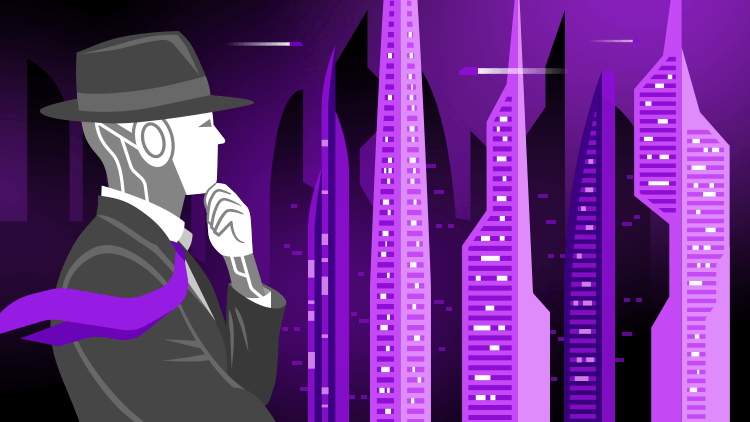
\includegraphics{Images/Course_Image.png}
		\end{center}
\end{figure}

\end{titlepage}

\renewcommand{\contentsname}{Tabla de Contenidos}
{
\setcounter{tocdepth}{1}
\tableofcontents
}

\newpage

\hypertarget{introducciuxf3n}{%
\chapter*{Introducción}\label{introducciuxf3n}}
\addcontentsline{toc}{chapter}{Introducción}

Este libro es el complemento de nuestro curso online \emph{Inteligencia Artificial aplicada a Negocios y Empresas} disponible en \href{https://www.udemy.com/ia4business/?couponCode=THEBOOK}{Udemy}. Cubre los tres casos prácticos de empresa reales que se resuelven, cada uno de ellos, con una técnica diferente del mundo de la inteligencia artificial:

\begin{longtable}[]{@{}ccc@{}}
\toprule
\begin{minipage}[b]{0.19\columnwidth}\centering
\textbf{Part}\strut
\end{minipage} & \begin{minipage}[b]{0.34\columnwidth}\centering
\textbf{Case Study}\strut
\end{minipage} & \begin{minipage}[b]{0.38\columnwidth}\centering
\textbf{AI Solution}\strut
\end{minipage}\tabularnewline
\midrule
\endhead
\begin{minipage}[t]{0.19\columnwidth}\centering
1 - Optimización de Procesos\strut
\end{minipage} & \begin{minipage}[t]{0.34\columnwidth}\centering
Optimizar el flujo en los almacenes de un ecommerce\strut
\end{minipage} & \begin{minipage}[t]{0.38\columnwidth}\centering
Q-Learning\strut
\end{minipage}\tabularnewline
\begin{minipage}[t]{0.19\columnwidth}\centering
2 - Minimización de Costes\strut
\end{minipage} & \begin{minipage}[t]{0.34\columnwidth}\centering
Minimizar los gastos de energía del servidor de un centro de datos\strut
\end{minipage} & \begin{minipage}[t]{0.38\columnwidth}\centering
Deep Q-Learning\strut
\end{minipage}\tabularnewline
\begin{minipage}[t]{0.19\columnwidth}\centering
3 - Maximización de Beneficios\strut
\end{minipage} & \begin{minipage}[t]{0.34\columnwidth}\centering
Mazimizar los beneficios de un negocio online de venta al por menor\strut
\end{minipage} & \begin{minipage}[t]{0.38\columnwidth}\centering
Muestreo Thompson\strut
\end{minipage}\tabularnewline
\bottomrule
\end{longtable}

En cada una de esas partes, seguiremos el mismo esquema de tres pasos:

\begin{itemize}
\tightlist
\item
  \textbf{Caso Práctico} Comenzaremos explicando el problema que tenemos que resolver y construiremos desde cero el entorno en el que trabajaremos.
\item
  \textbf{AI Solution.} Te daremos no solo la teoría general sino también todos los detalles matemáticos del modelo de IA que resolverán el caso práctico
\item
  \textbf{Implementation.} Implementaremos toda la solución de inteligencia artificial en Python, lo pondremos en producción y mejoraremos la inteligencia artificial al completar tareas adicionales al final.
\end{itemize}

¡Muchas gracias a todos por unirte a nosotros en este curso, te deseo sin duda un emocionante viaje al mundo de la IA aplicada a Negocios y Empresas con nosotros!

\hypertarget{optimizaciuxf3n-de-procesos}{%
\chapter{Optimización de Procesos}\label{optimizaciuxf3n-de-procesos}}

Aquí vamos con nuestro primer caso práctico y nuestro primer modelo de IA. ¡Esperamos que estés listo!

\hypertarget{caso-pruxe1ctico-optimizaciuxf3n-de-tareas-en-un-almacuxe9n-de-comercio-electruxf3nico}{%
\section{Caso Práctico: Optimización de tareas en un almacén de comercio electrónico}\label{caso-pruxe1ctico-optimizaciuxf3n-de-tareas-en-un-almacuxe9n-de-comercio-electruxf3nico}}

\hypertarget{problema-a-resolver}{%
\subsection{Problema a resolver}\label{problema-a-resolver}}

El problema a resolver será optimizar los flujos dentro del siguiente almacén:

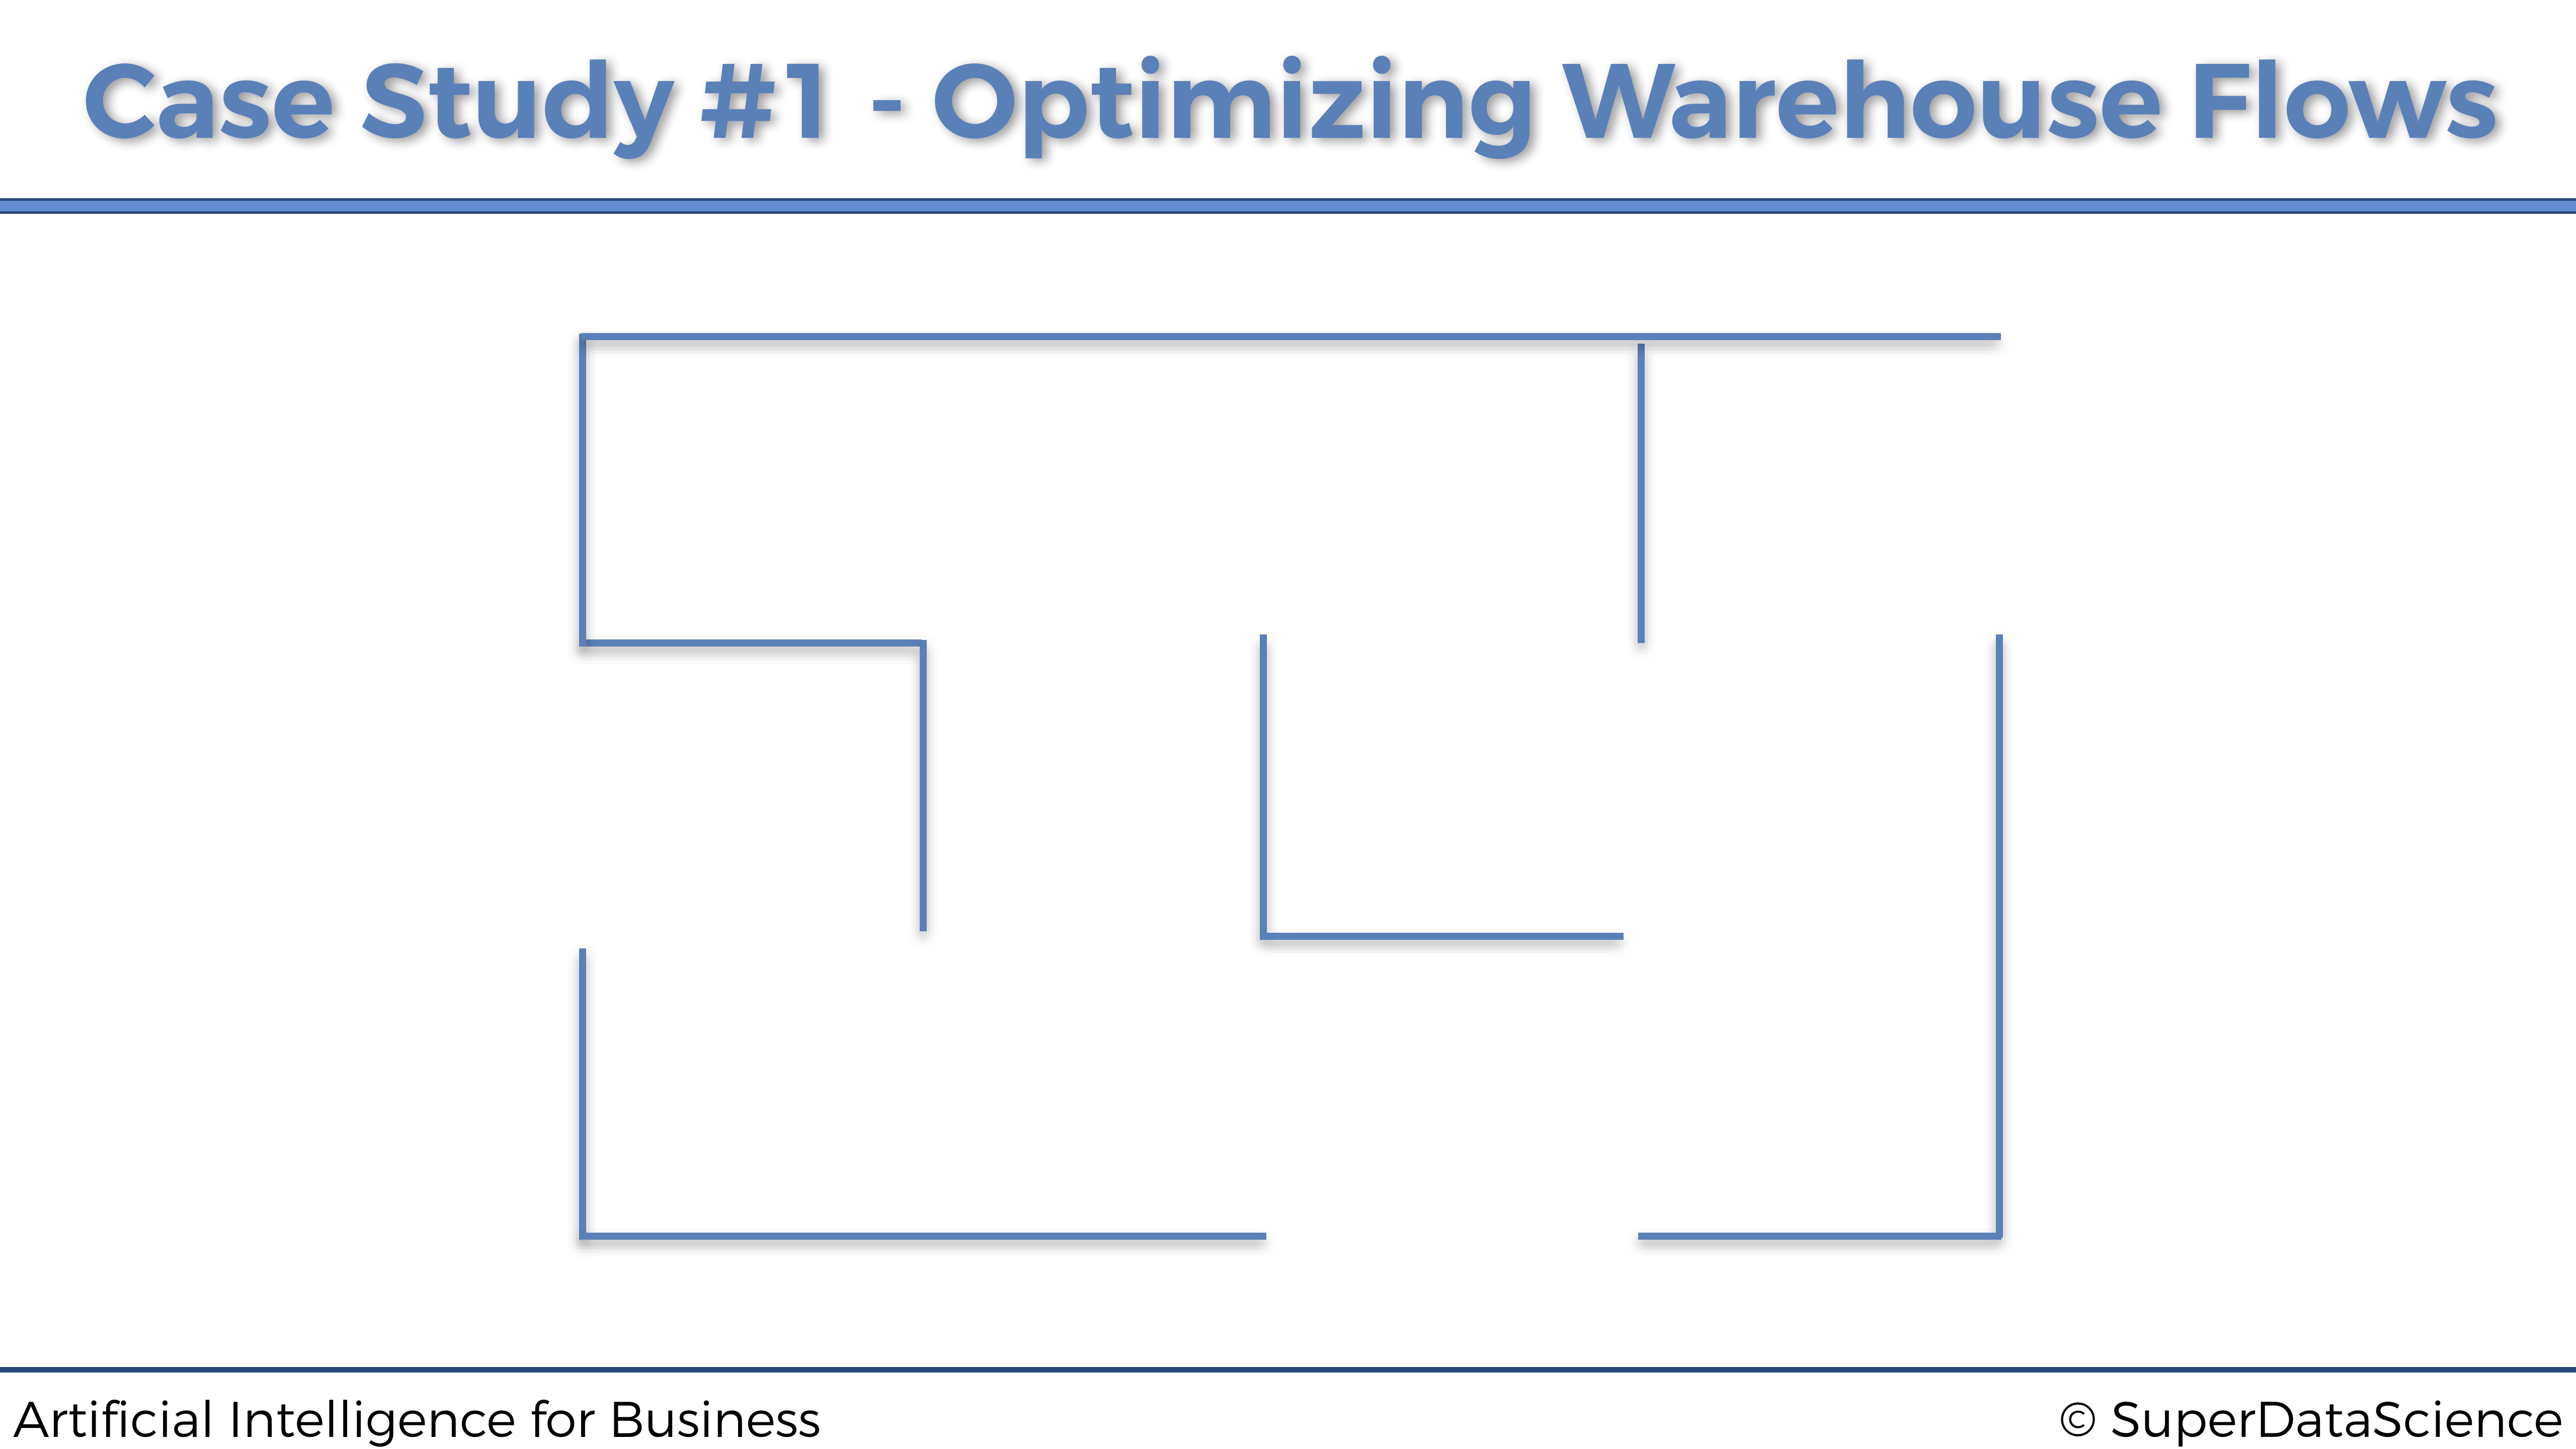
\includegraphics[width=1\textwidth,height=\textheight]{Images/Warehouse_1.png}

El almacén pertenece a una empresa online minorista que vende productos a una variedad de clientes. Dentro de este almacén, los productos se almacenan en 12 ubicaciones diferentes, etiquetadas con las siguientes letras de la A a la L:

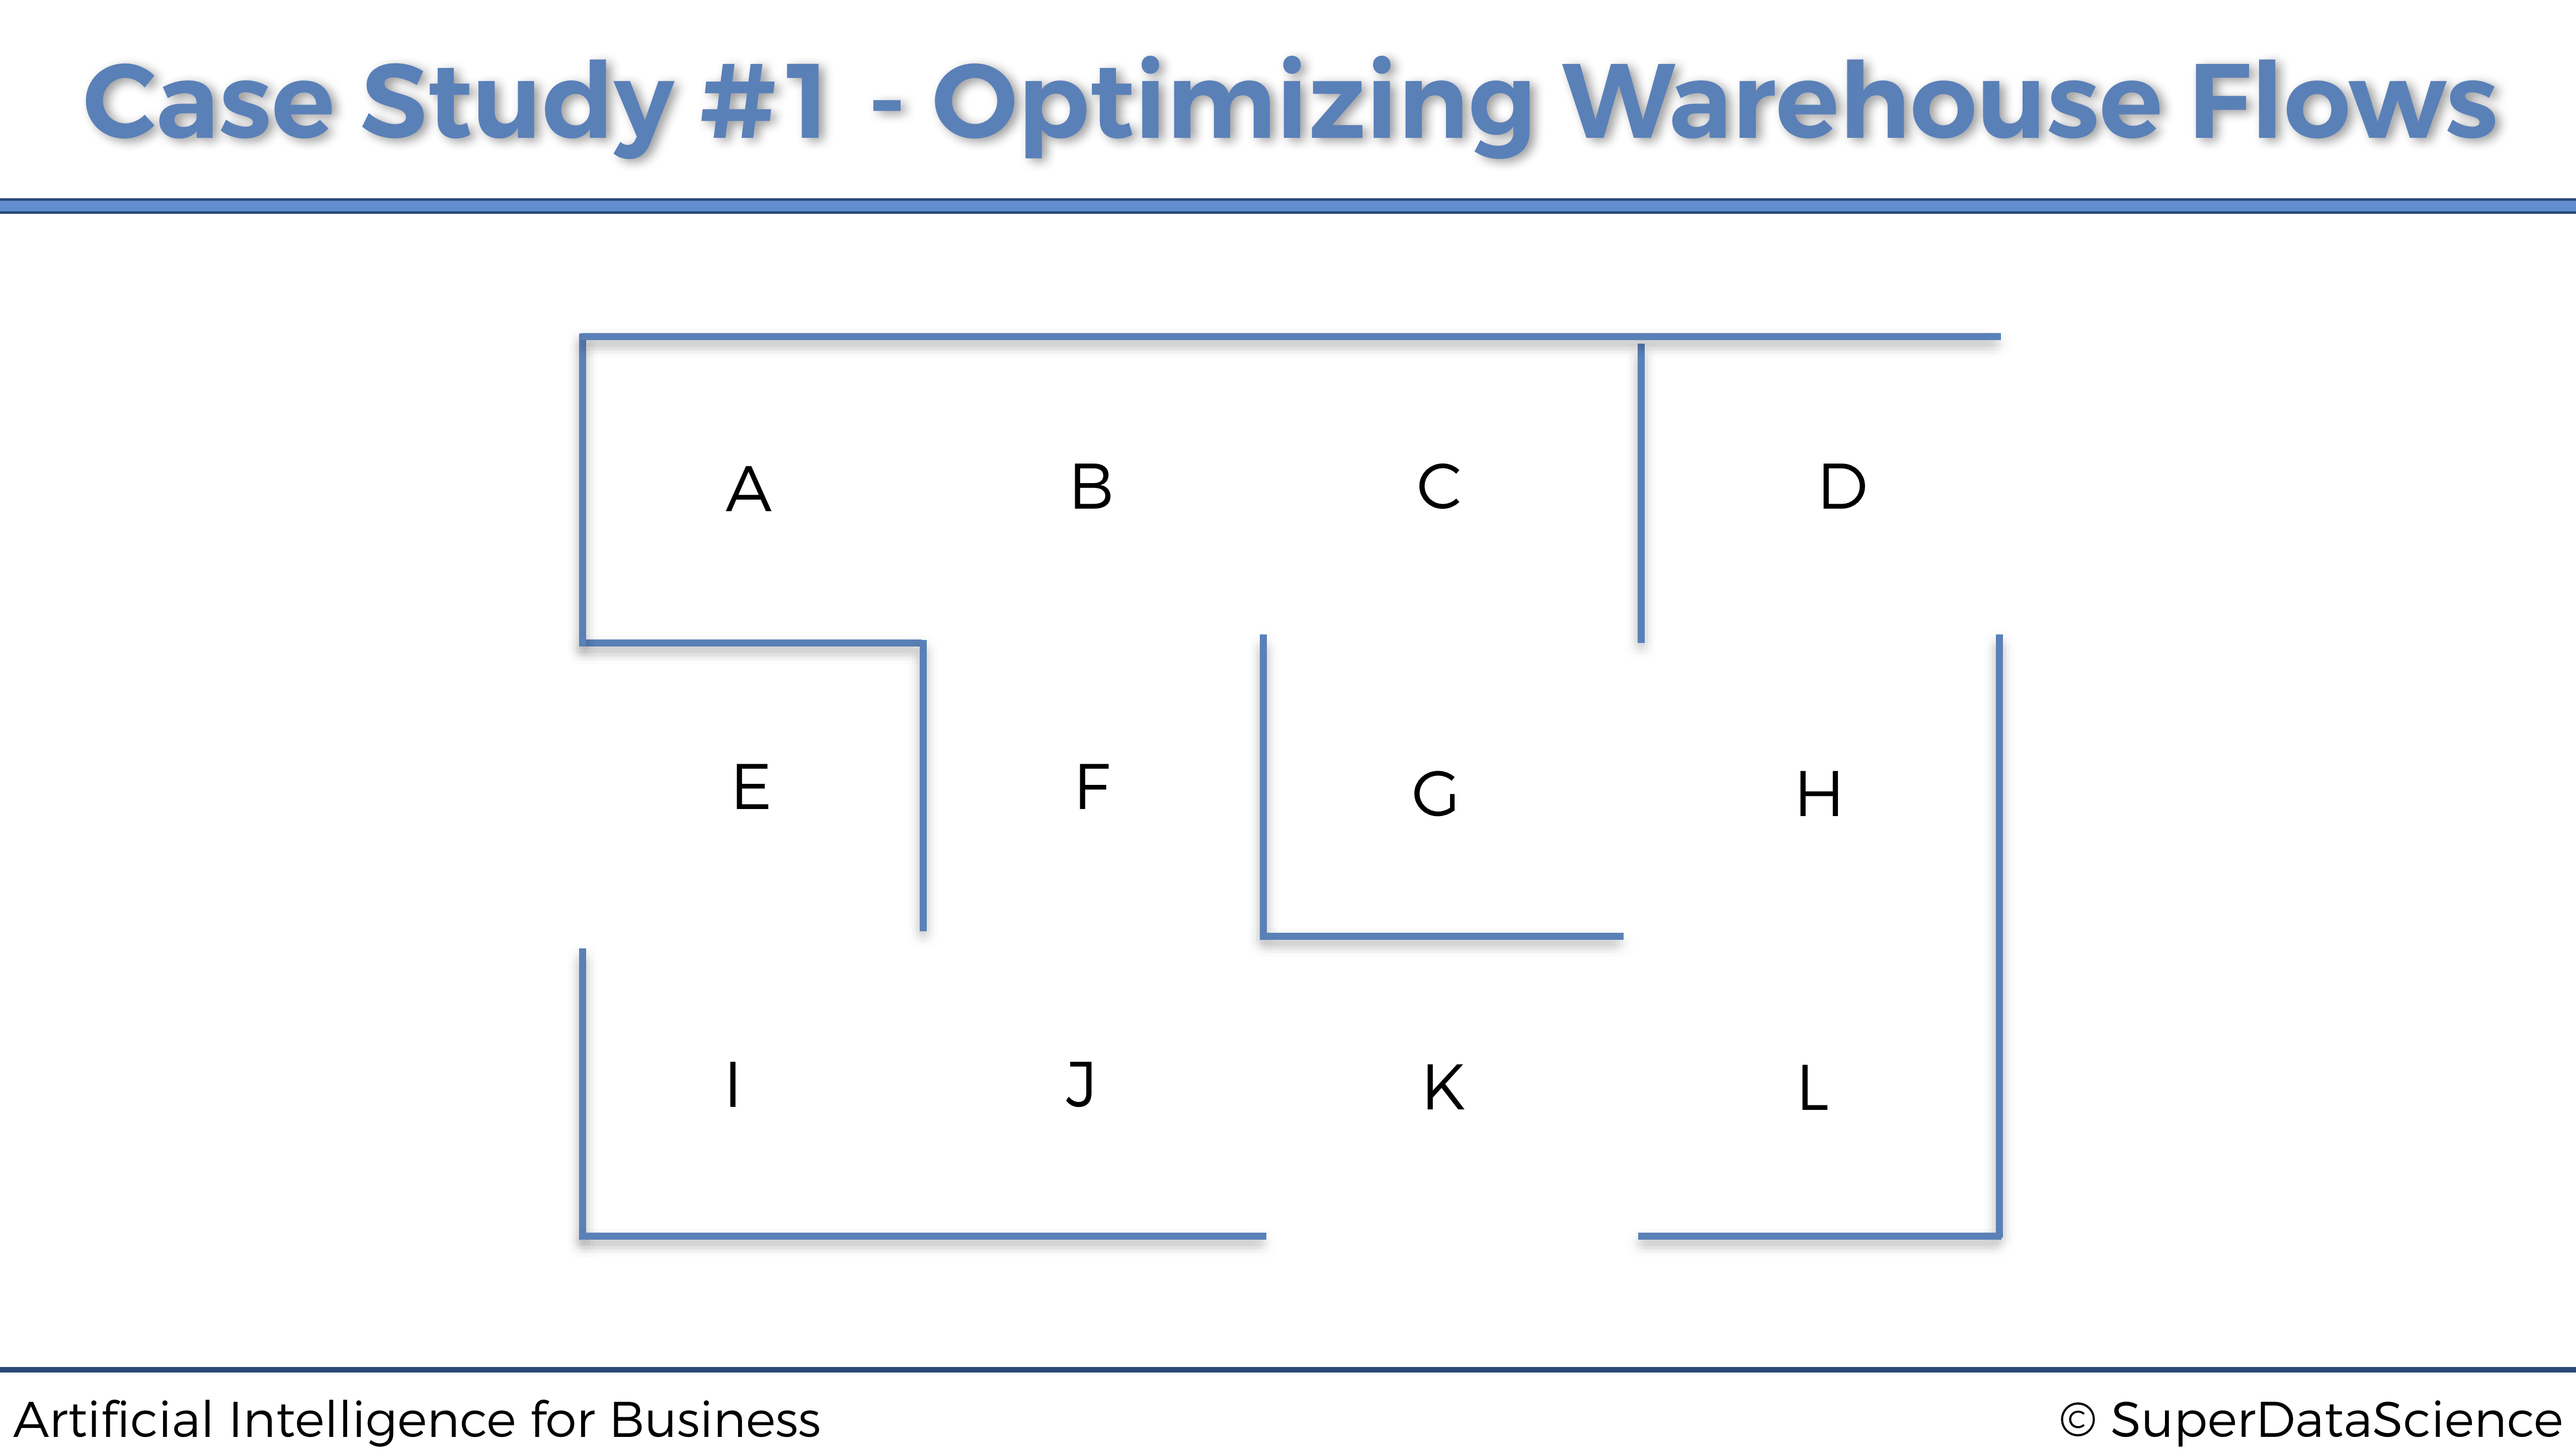
\includegraphics[width=1\textwidth,height=\textheight]{Images/Warehouse_2.png}

A medida que los clientes hacen los pedidos online, un robot de almacén autónomo se mueve por el almacén para recoger los productos para futuras entregas. Así es como se ve:

\begin{figure}
\centering
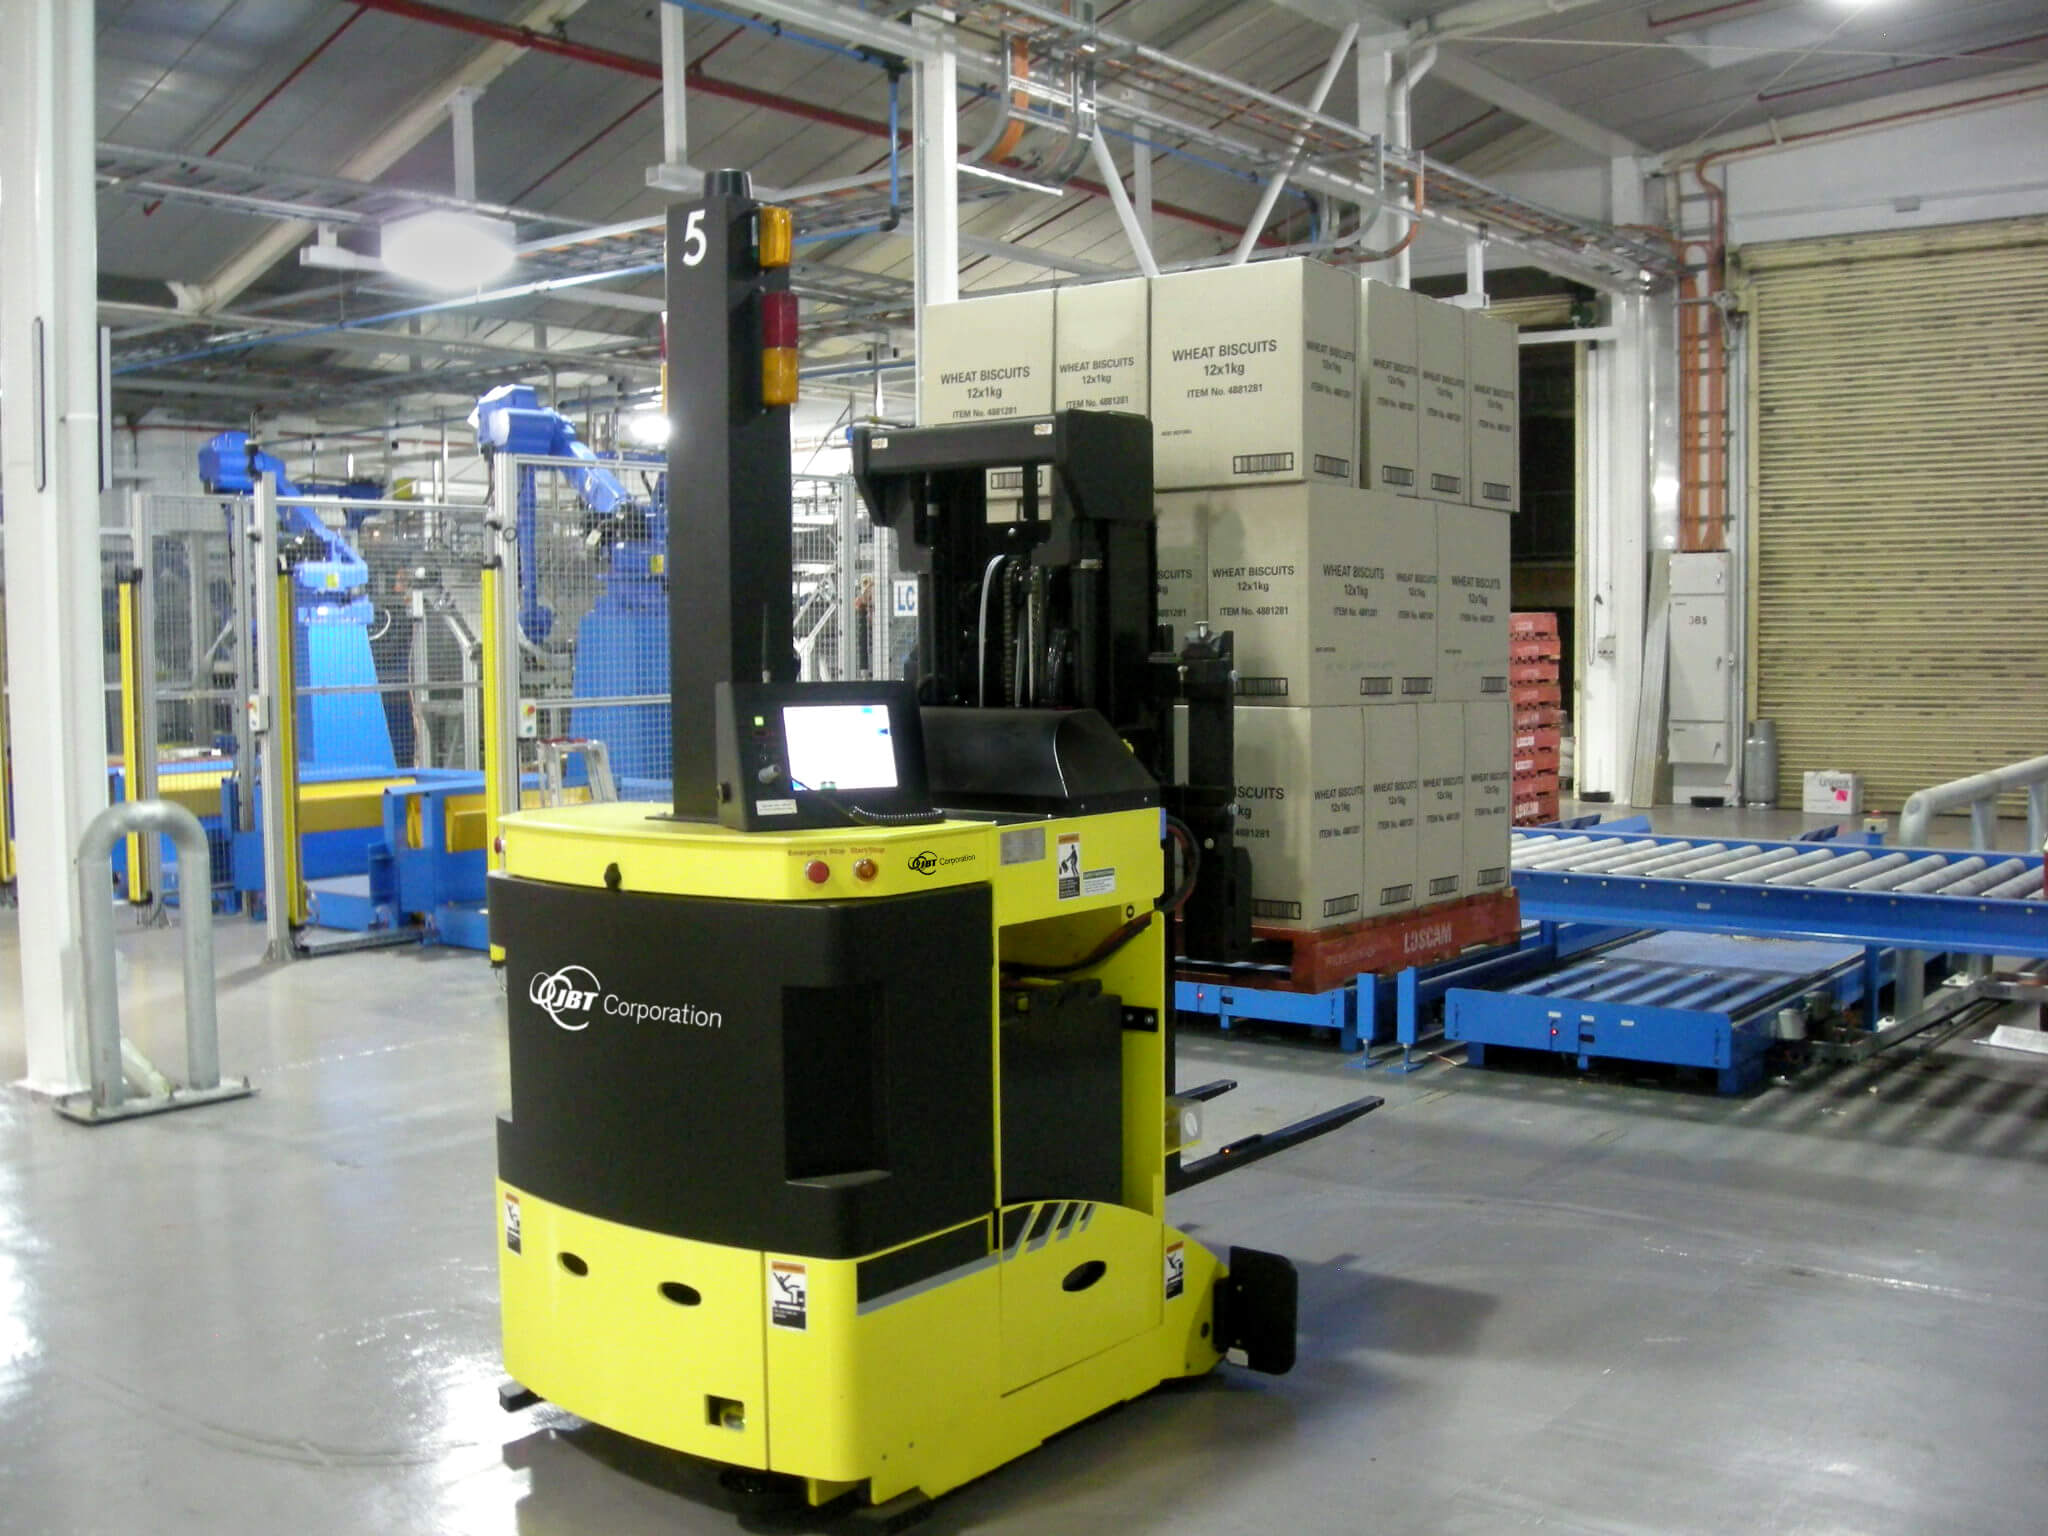
\includegraphics[width=1\textwidth,height=\textheight]{Images/Autonomous_Warehouse_Robot.jpg}
\caption{Robot de Almacen Autónomo}
\end{figure}

Las 12 ubicaciones están conectadas a un sistema informático, que clasifica en tiempo real las prioridades de recolección de productos para estas 12 ubicaciones. Por ejemplo, en un momento específico \(t\), devolverá la siguiente clasificación:

\begin{longtable}[]{@{}cc@{}}
\toprule
\textbf{Rango de Prioridad} & \textbf{Ubicación}\tabularnewline
\midrule
\endhead
1 & G\tabularnewline
2 & K\tabularnewline
3 & L\tabularnewline
4 & J\tabularnewline
5 & A\tabularnewline
6 & I\tabularnewline
7 & H\tabularnewline
8 & C\tabularnewline
9 & B\tabularnewline
10 & D\tabularnewline
11 & F\tabularnewline
12 & E\tabularnewline
\bottomrule
\end{longtable}

La ubicación G tiene prioridad 1, lo que significa que es la máxima prioridad, ya que contiene un producto que debe recogerse y entregarse de inmediato. Nuestro robot de almacén autónomo debe moverse a la ubicación G por la ruta más corta, dependiendo de dónde se encuentre. Nuestro objetivo es construir una IA que regrese esa ruta más corta, donde sea que esté el robot. Pero luego, como vemos, las ubicaciones K y L están en las 3 prioridades principales. Por lo tanto, querremos implementar una opción para que nuestro Robot de almacén autónomo pase por algunas ubicaciones intermedias antes de llegar a su ubicación final de máxima prioridad.

La forma en que el sistema calcula las prioridades de las ubicaciones está fuera del alcance de este caso práctico. La razón de esto es que puede haber muchas formas, desde reglas o algoritmos simples, hasta cálculos deterministas y aprendizaje automático. Pero la mayoría de estas formas no serían inteligencia artificial como la conocemos hoy. En lo que realmente queremos centrarnos es en la IA central, que abarca Q-Learning, Deep Q-Learning y otras ramas de Reinforcement Learning. Entonces, solo diremos, por ejemplo, que la ubicación G es la máxima prioridad porque uno de los clientes de platino más leales de la compañía hizo un pedido urgente de un producto almacenado en la ubicación G, que por lo tanto debe entregarse lo antes posible.

Por lo tanto, en conclusión, nuestra misión es construir una IA que siempre tome la ruta más corta a la ubicación de máxima prioridad, sea cual sea la ubicación desde la que comienza, y tener la opción de ir a una ubicación intermedia que se encuentre entre las 3 prioridades principales.

\hypertarget{entorno-a-definir}{%
\subsection{Entorno a definir}\label{entorno-a-definir}}

Al construir una IA, lo primero que siempre tenemos que hacer es definir el entorno. Y definir un entorno siempre requiere los tres elementos siguientes:

\begin{itemize}
\tightlist
\item
  Definir los estados
\item
  Definir las acciones
\item
  Definir las recompensas
\end{itemize}

Definamos estos tres elementos, uno por uno.

\textbf{Definir los estados.}

Comencemos con los estados. El estado de entrada es simplemente la ubicación donde está nuestro Robot de almacén autónomo en cada momento \(t\). Sin embargo, dado que construiremos nuestra IA con ecuaciones matemáticas, codificaremos los nombres de las ubicaciones (A, B, C, \ldots{}) en números de índice, con respecto a la siguiente asignación:

\begin{longtable}[]{@{}cc@{}}
\toprule
\textbf{Ubicación} & \textbf{Estado}\tabularnewline
\midrule
\endhead
A & 0\tabularnewline
B & 1\tabularnewline
C & 2\tabularnewline
D & 3\tabularnewline
E & 4\tabularnewline
F & 5\tabularnewline
G & 6\tabularnewline
H & 7\tabularnewline
I & 8\tabularnewline
J & 9\tabularnewline
K & 10\tabularnewline
L & 11\tabularnewline
\bottomrule
\end{longtable}

Hay una razón específica por la que codificamos los estados con índices del 0 al 11, en lugar de otros enteros. La razón es que trabajaremos con matrices, una matriz de recompensas y una matriz de valores Q, y cada línea y columna de estas matrices corresponderá a una ubicación específica. Por ejemplo, la primera línea de cada matriz, que tiene el índice 0, corresponde a la ubicación A. La segunda línea / columna, que tiene el índice 1, corresponde a la ubicación B. Etc. Veremos el propósito de trabajar con matrices con más detalles. un poco más tarde.

\textbf{Definir las acciones.}

Ahora definamos las posibles acciones a realizar Las acciones son simplemente los siguientes movimientos que el robot puede hacer para ir de un lugar a otro. Entonces, por ejemplo, digamos que el robot está en la ubicación J, las posibles acciones que el robot puede llevar a cabo es ir a I, F o K. Y nuevamente, ya que trabajaremos con ecuaciones matemáticas, codificaremos estas acciones con los mismos índices que para los estados. Por lo tanto, siguiendo nuestro mismo ejemplo donde el robot está en la ubicación J en un momento específico, las posibles acciones que el robot puede jugar son, de acuerdo con nuestro mapeo anterior anterior: 5, 8 y 10. De hecho, el índice 5 corresponde a F, el índice 8 corresponde a I y el índice 10 corresponde a K. Por lo tanto, eventualmente, la lista total de acciones que la IA puede llevar a cabo en general es la siguiente:

\[actions = [0,1,2,3,4,5,6,7,8,9,10,11]\]

Obviamente, al estar en una ubicación específica, hay algunas acciones que el robot no puede llevar a cabo. Tomando el mismo ejemplo anterior, si el robot está en la ubicación J, puede ejecutar las acciones 5, 8 y 10, pero no puede ejecutar las otras acciones. Nos aseguraremos de especificar eso al atribuir una recompensa 0 a las acciones que no puede llevar a cabo, y una recompensa 1 a las acciones que si puede realizar. Y eso nos lleva a las recompensas.

\textbf{Definir las recompensas.}

Lo último que tenemos que hacer ahora para construir nuestro entorno es definir un sistema de recompensas. Más específicamente, tenemos que definir una función de recompensa \(R\) que toma como entradas un estado \(s\) y una acción \(a\), y devuelve una recompensa numérica que la IA obtendrá al llevar a cabo la acción \(a\) en el estado \(s\):

\[R : (\textrm{state}, \textrm{action}) \mapsto r \in \mathbb{R}\]

Entonces, ¿cómo vamos a construir esa función para nuestro caso práctico? Aquí esto es simple. Dado que hay un número discreto y finito de estados (los índices de 0 a 11), así como un número discreto y finito de acciones (mismos índices de 0 a 11), la mejor manera de construir nuestra función de recompensa R es simplemente hacer una matriz. Nuestra función de recompensa será exactamente una matriz de 12 filas y 12 columnas, donde las filas corresponden a los estados y las columnas corresponden a las acciones. De esa forma, en nuestra función \$R: (s, a) \mapsto r ~in \mathbb{R} \$, \(s\) será el índice de la fila de la matriz, \(a\) será el índice de la columna de matriz, y \(r\) será la celda de los índices \((s, a)\) en la matriz.

Por lo tanto, lo único que tenemos que hacer ahora para definir nuestra función de recompensa es simplemente llenar esta matriz con las recompensas numéricas. Y como acabamos de decir en el párrafo anterior, lo que tenemos que hacer primero es atribuir, para cada una de las 12 ubicaciones, una recompensa 0 por las acciones que el robot no puede ejecutar, y una recompensa 1 por las acciones que el robot puede llevar a cabo. Al hacer eso para cada una de las 12 ubicaciones, terminaremos con una matriz de recompensas. Vamos a construirlo paso a paso, comenzando con la primera ubicación:

\emph{Ubicación A.}

Cuando se encuentra en la ubicación A, el robot solo puede ir a la ubicación B. Por lo tanto, dado que la ubicación A tiene el índice 0 (primera fila de la matriz) y la ubicación B tiene el índice 1 (segunda columna de la matriz), la primera fila de la matriz de las recompensas obtendrá un 1 en la segunda columna y un 0 en todas las otras columnas, así:

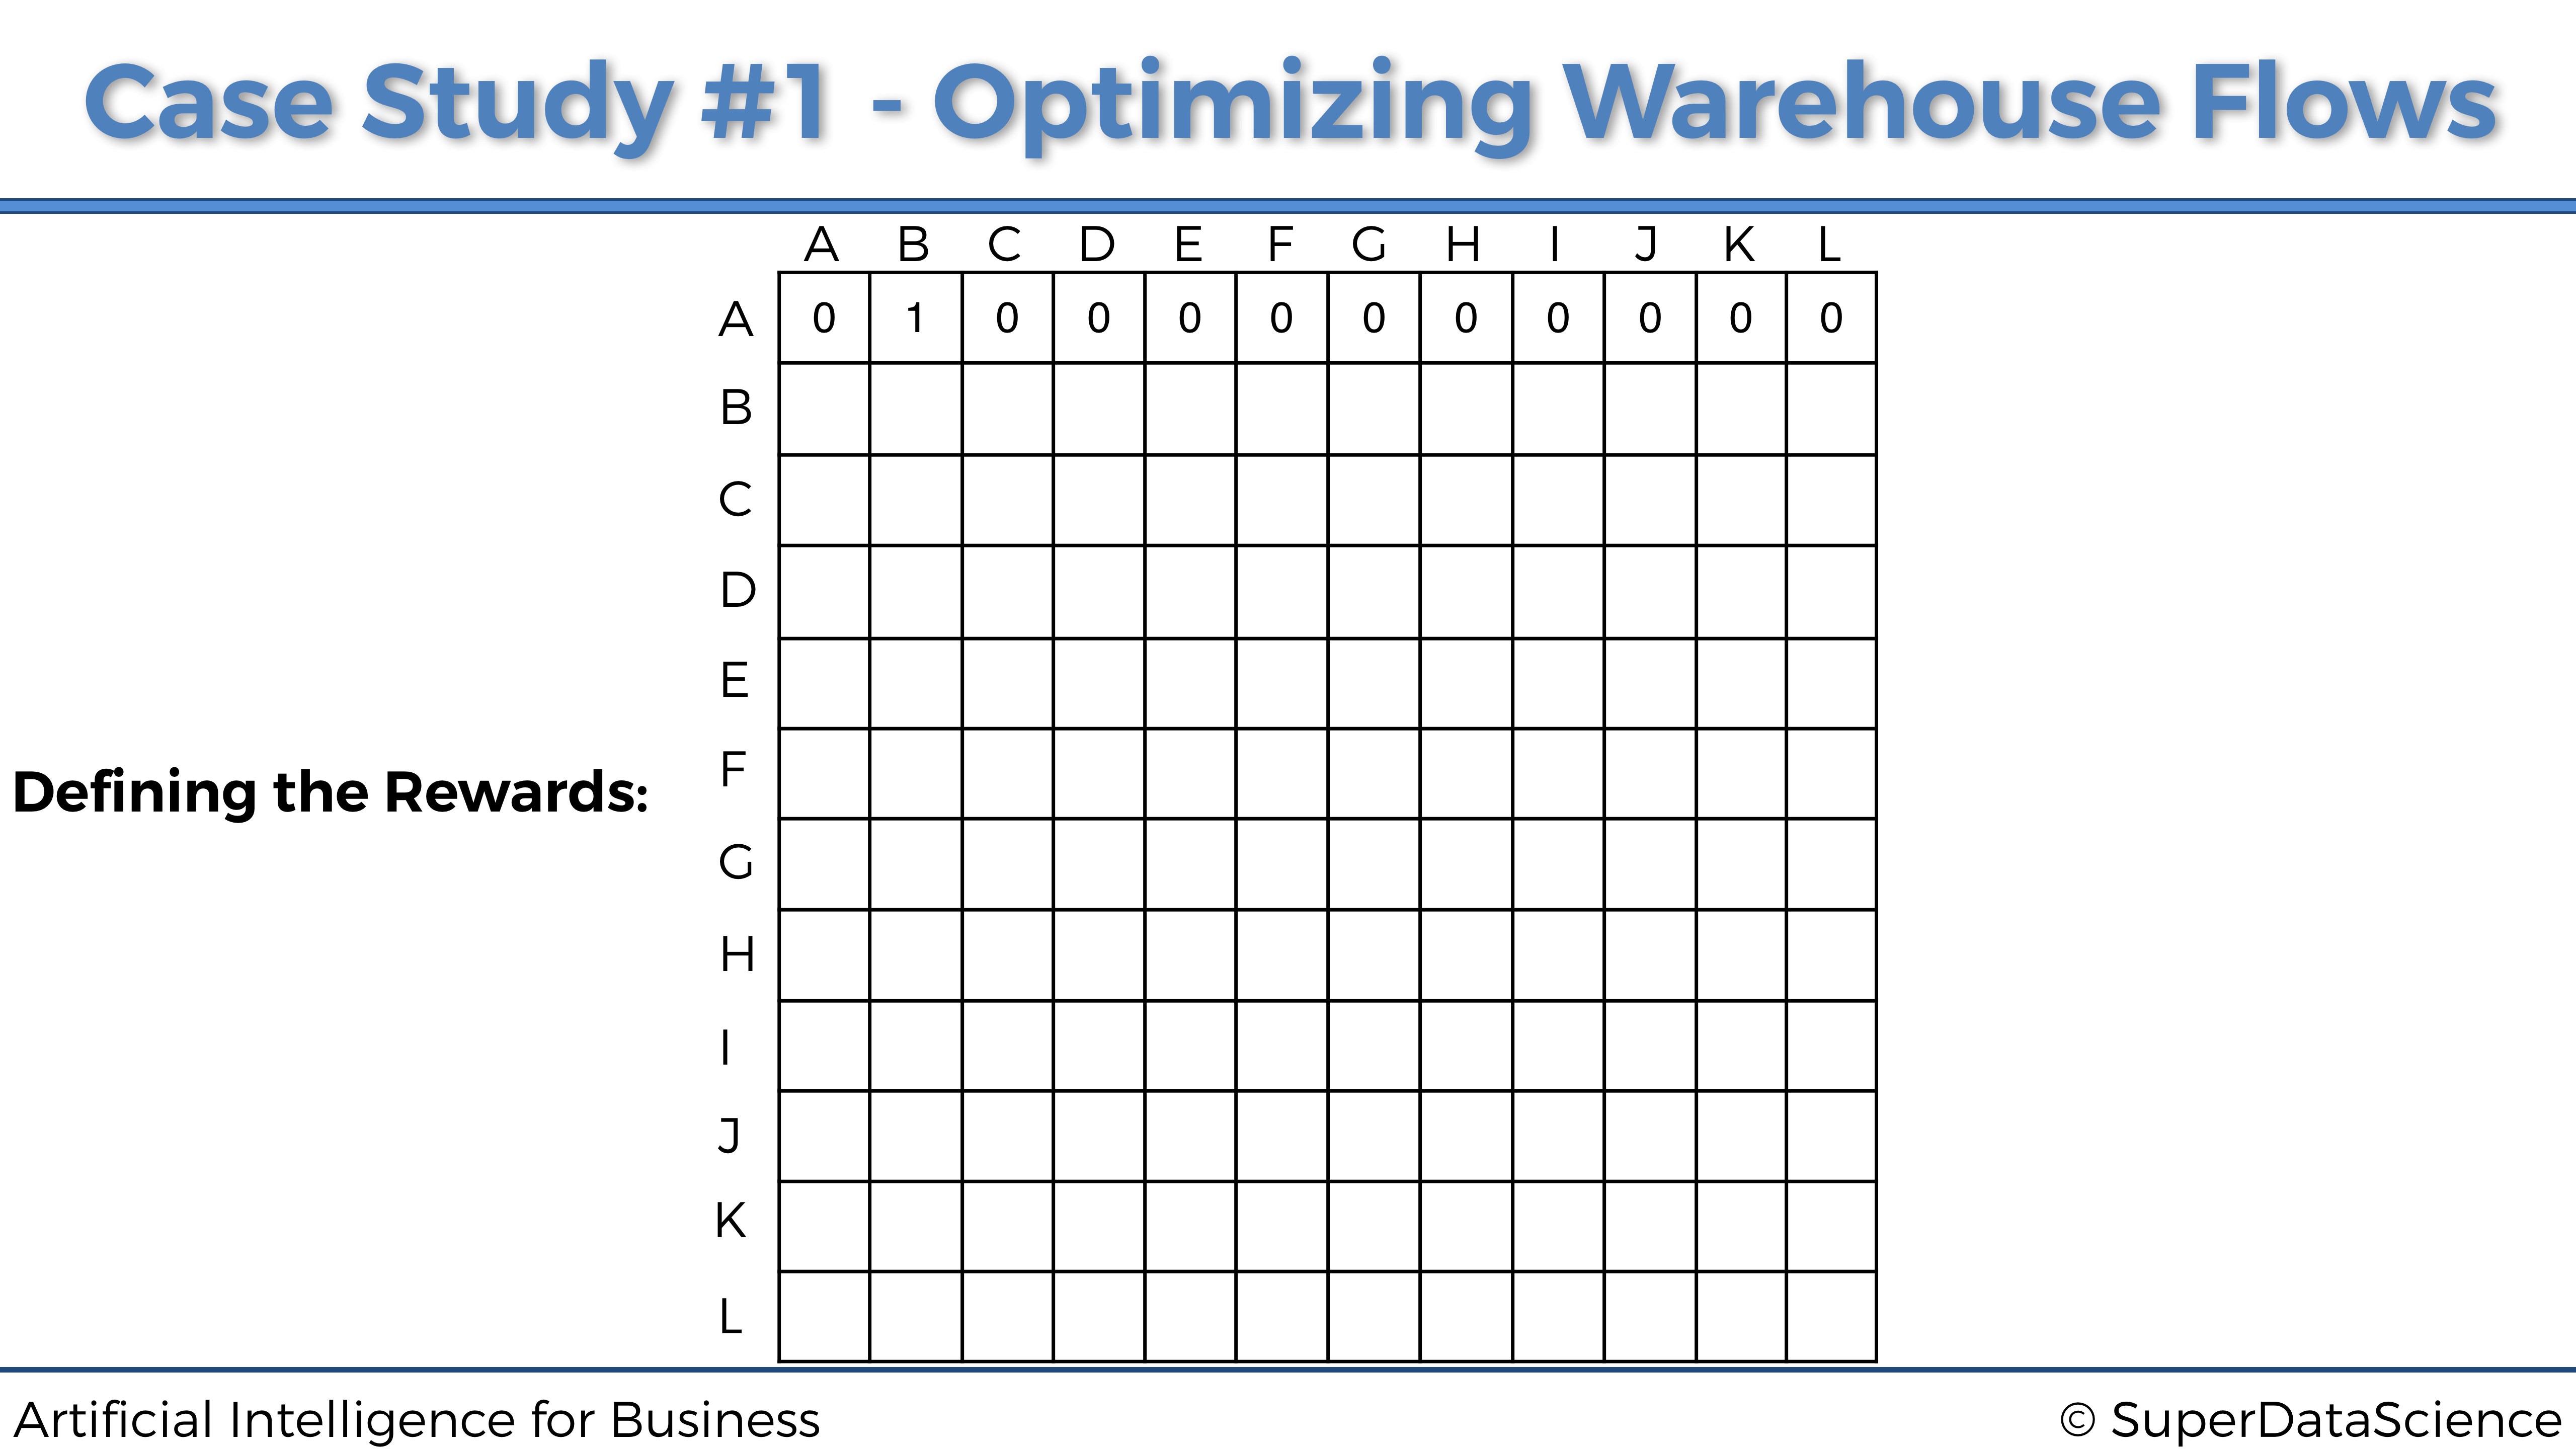
\includegraphics{Images/Rewards_Matrix_1.png}

\emph{Ubicación B.}

Al estar en la ubicación B, el robot solo puede ir a tres ubicaciones diferentes: A, C y F. Dado que B tiene el índice 1 (segunda fila), y A, C, F tienen los índices respectivos 0, 2, 5 (1ra, 3ra. , y sexta columna), entonces la segunda fila de la matriz de recompensas obtendrá un 1 en las columnas 1a, 3a y 6a, y 0 en todas las otras columnas. Por lo tanto obtenemos:

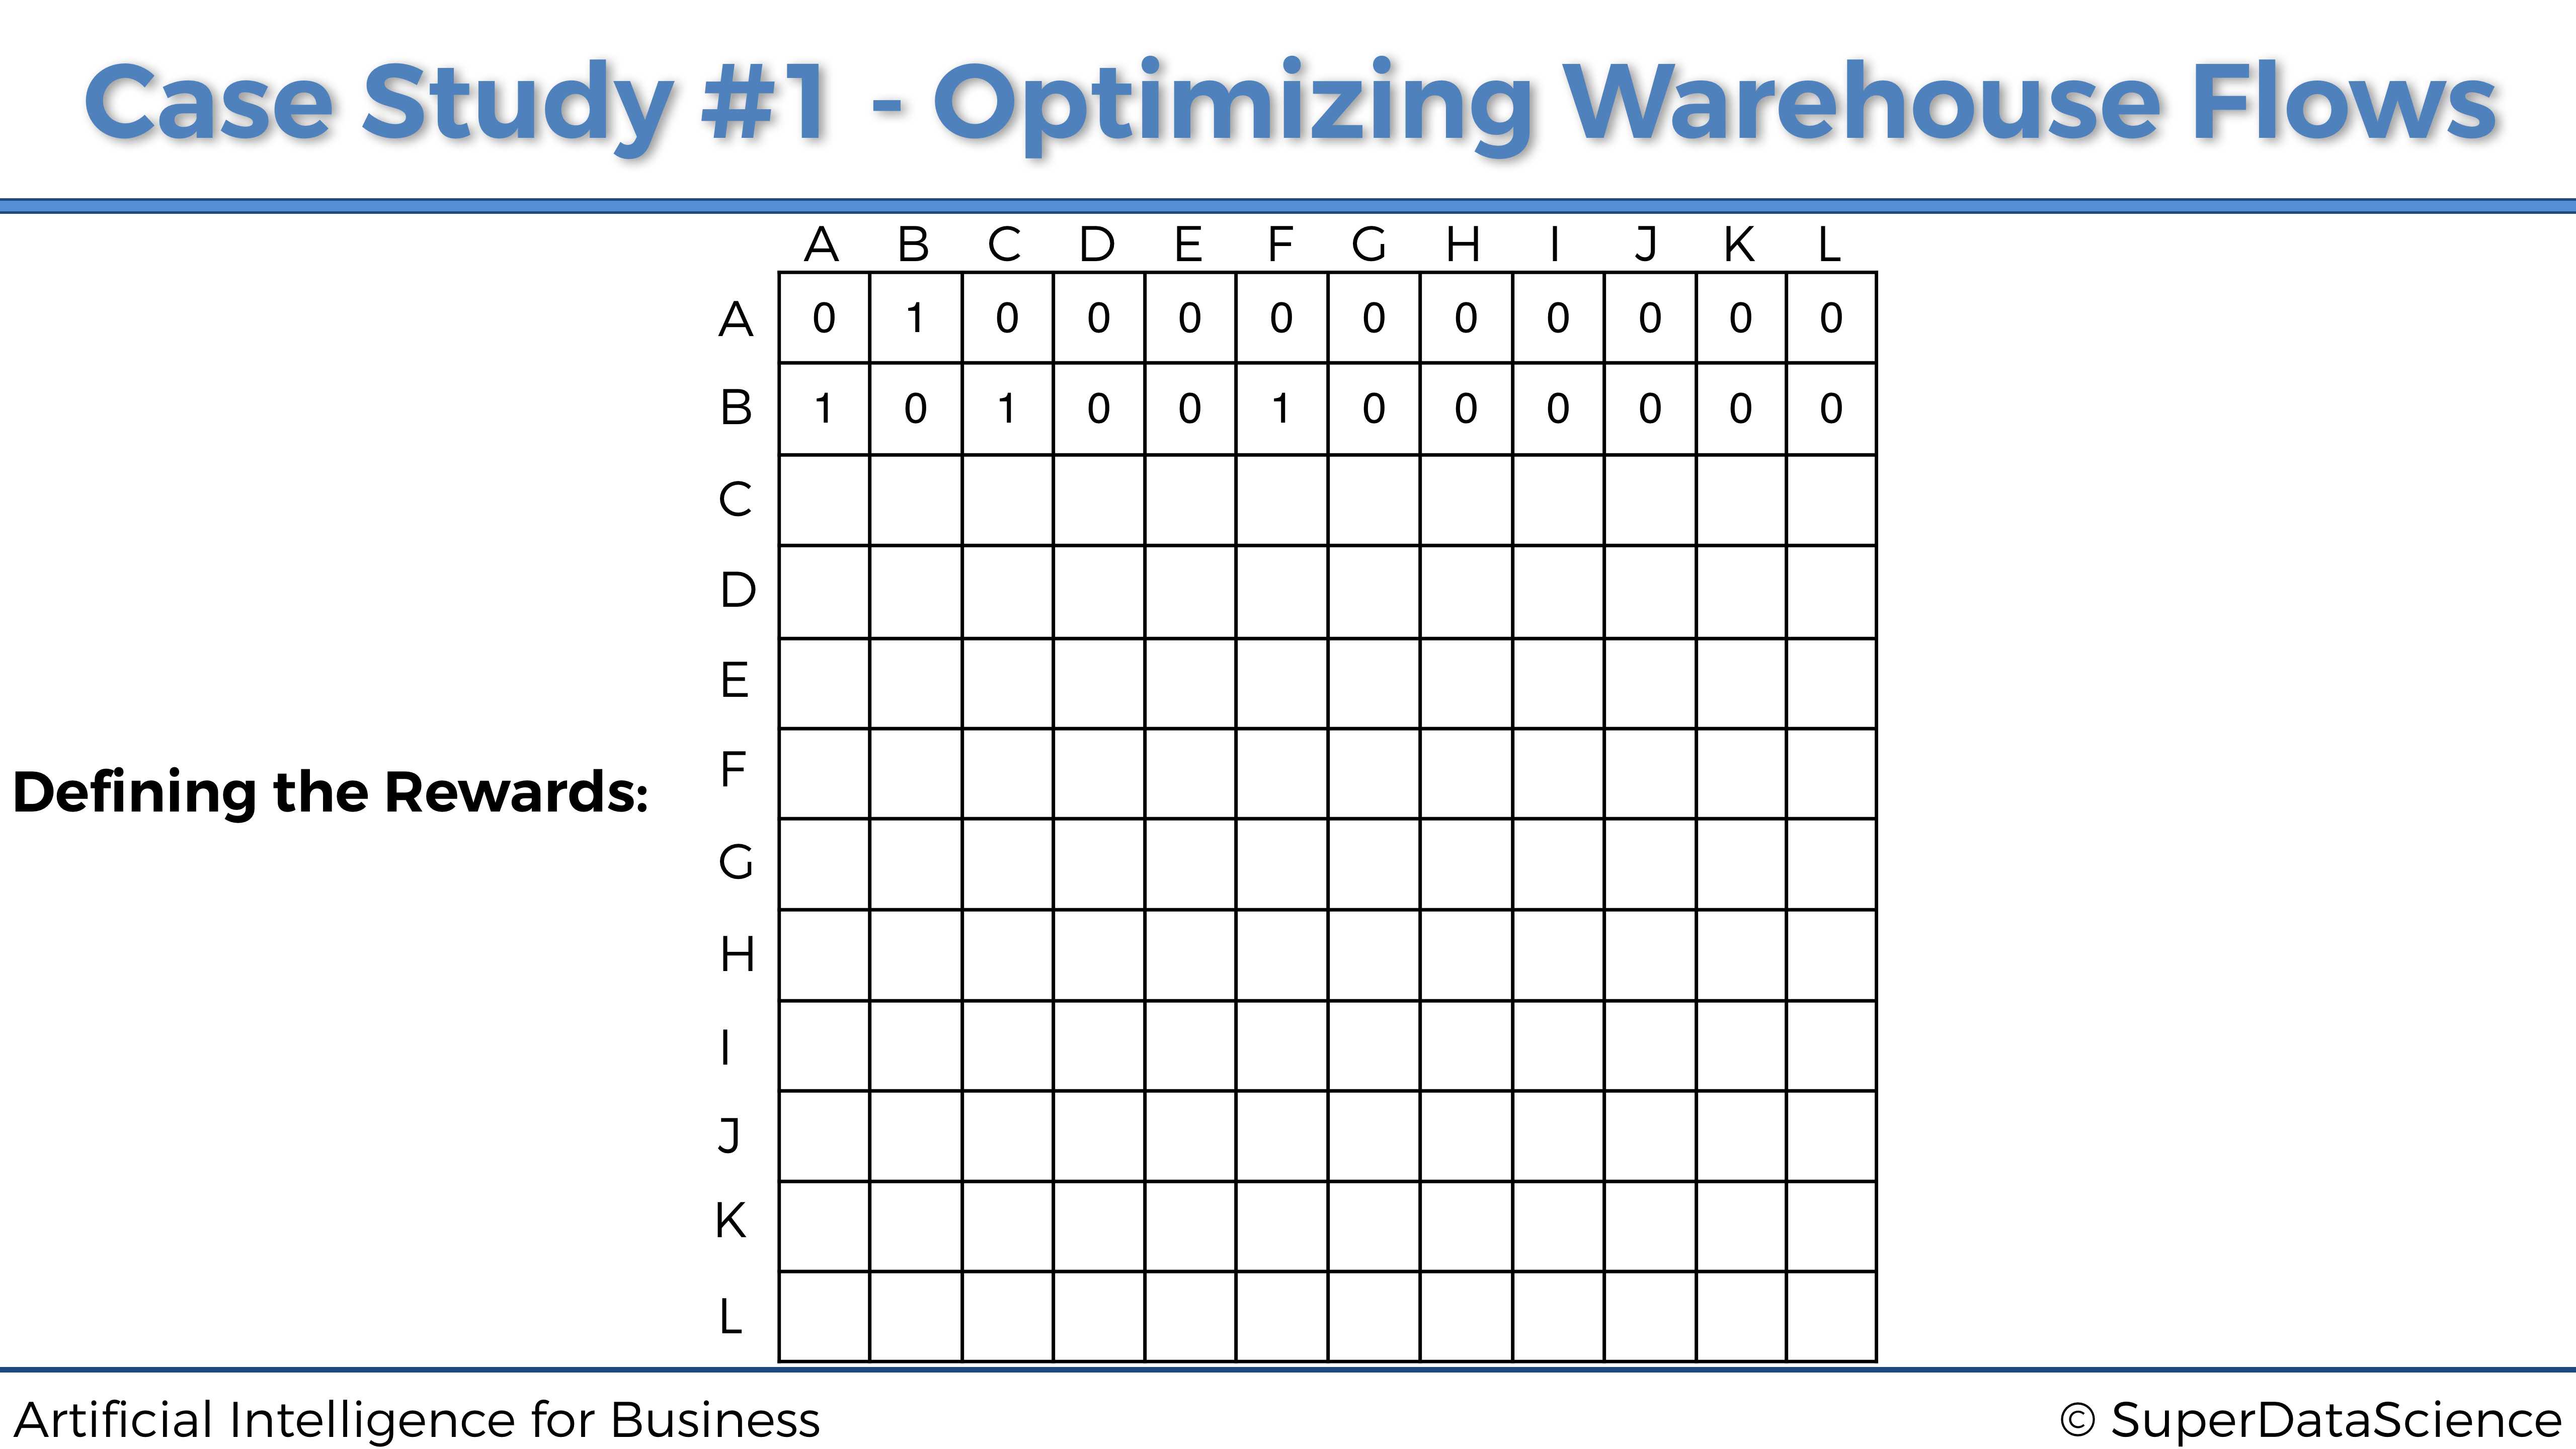
\includegraphics{Images/Rewards_Matrix_2.png}

\emph{Ubicación C.}

Ocurre lo mismo, la ubicación C (de índice 2) solo está conectada a B y G (de índices 1 y 6), por lo que la tercera fila de la matriz de recompensas es:

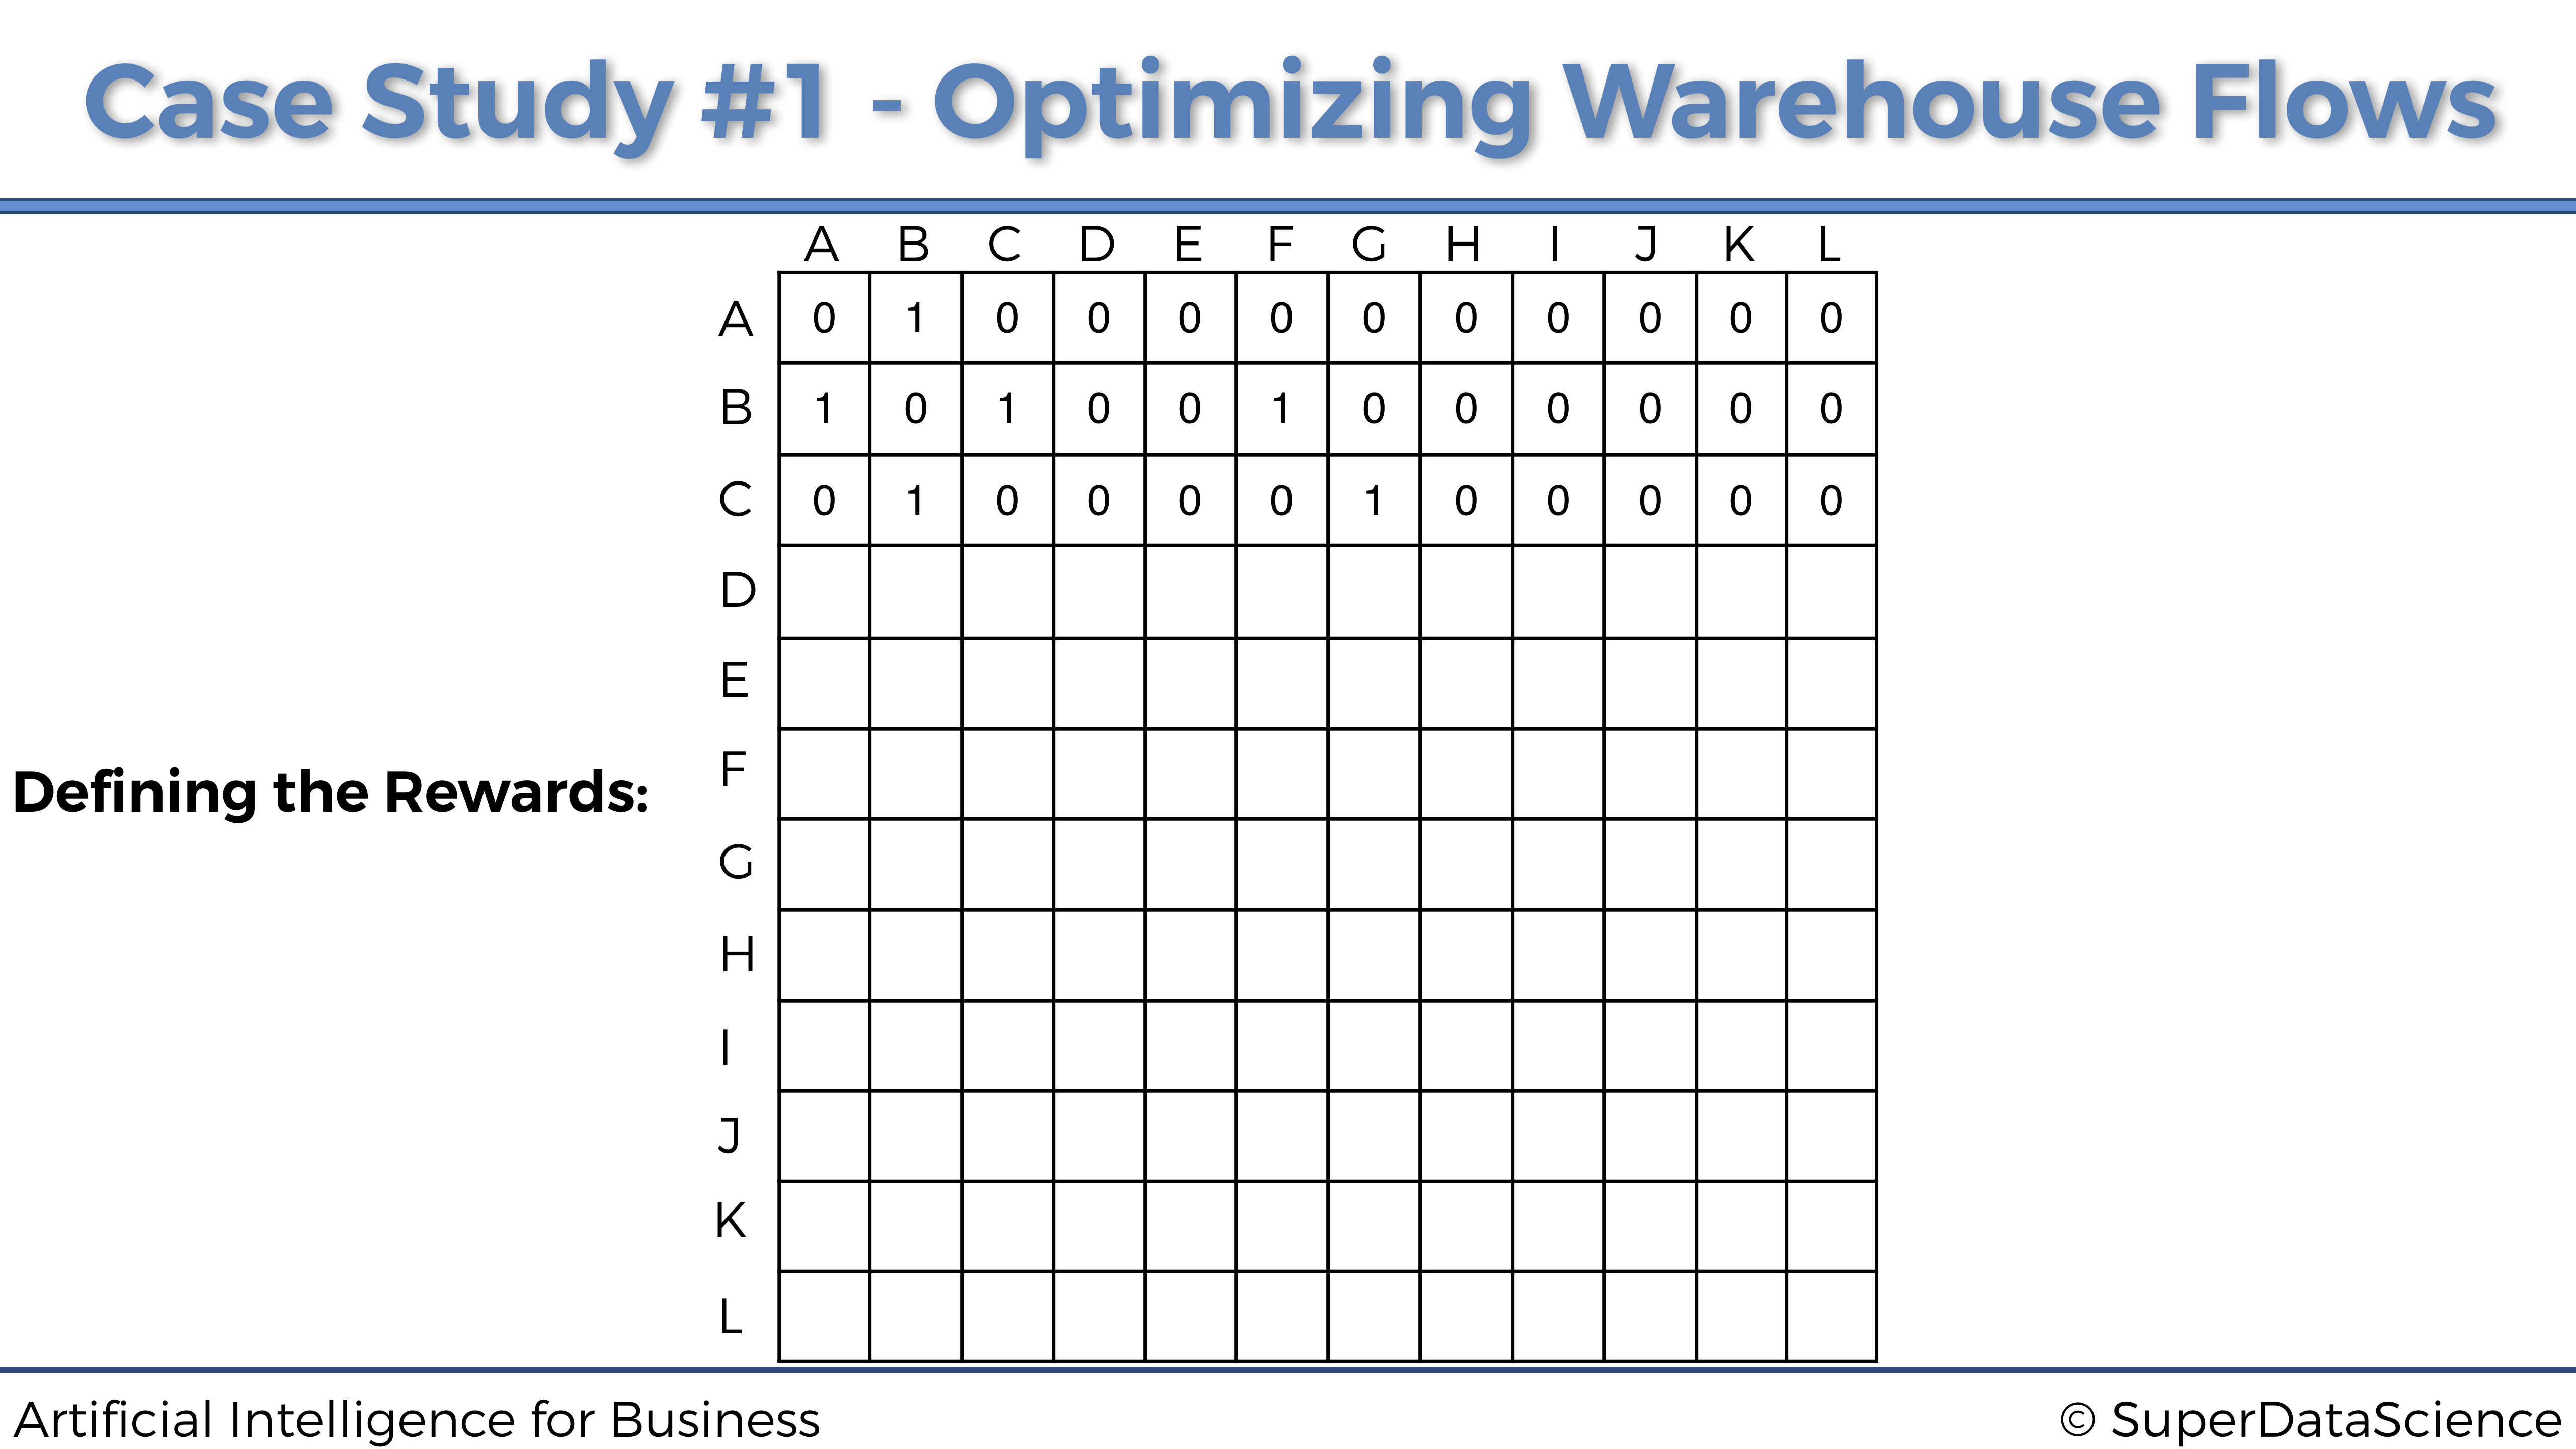
\includegraphics{Images/Rewards_Matrix_3.png}

\emph{En el resto de ubicaciones\ldots{}}

Al hacer lo mismo para todas las demás ubicaciones, finalmente obtenemos nuestra matriz final de recompensas:

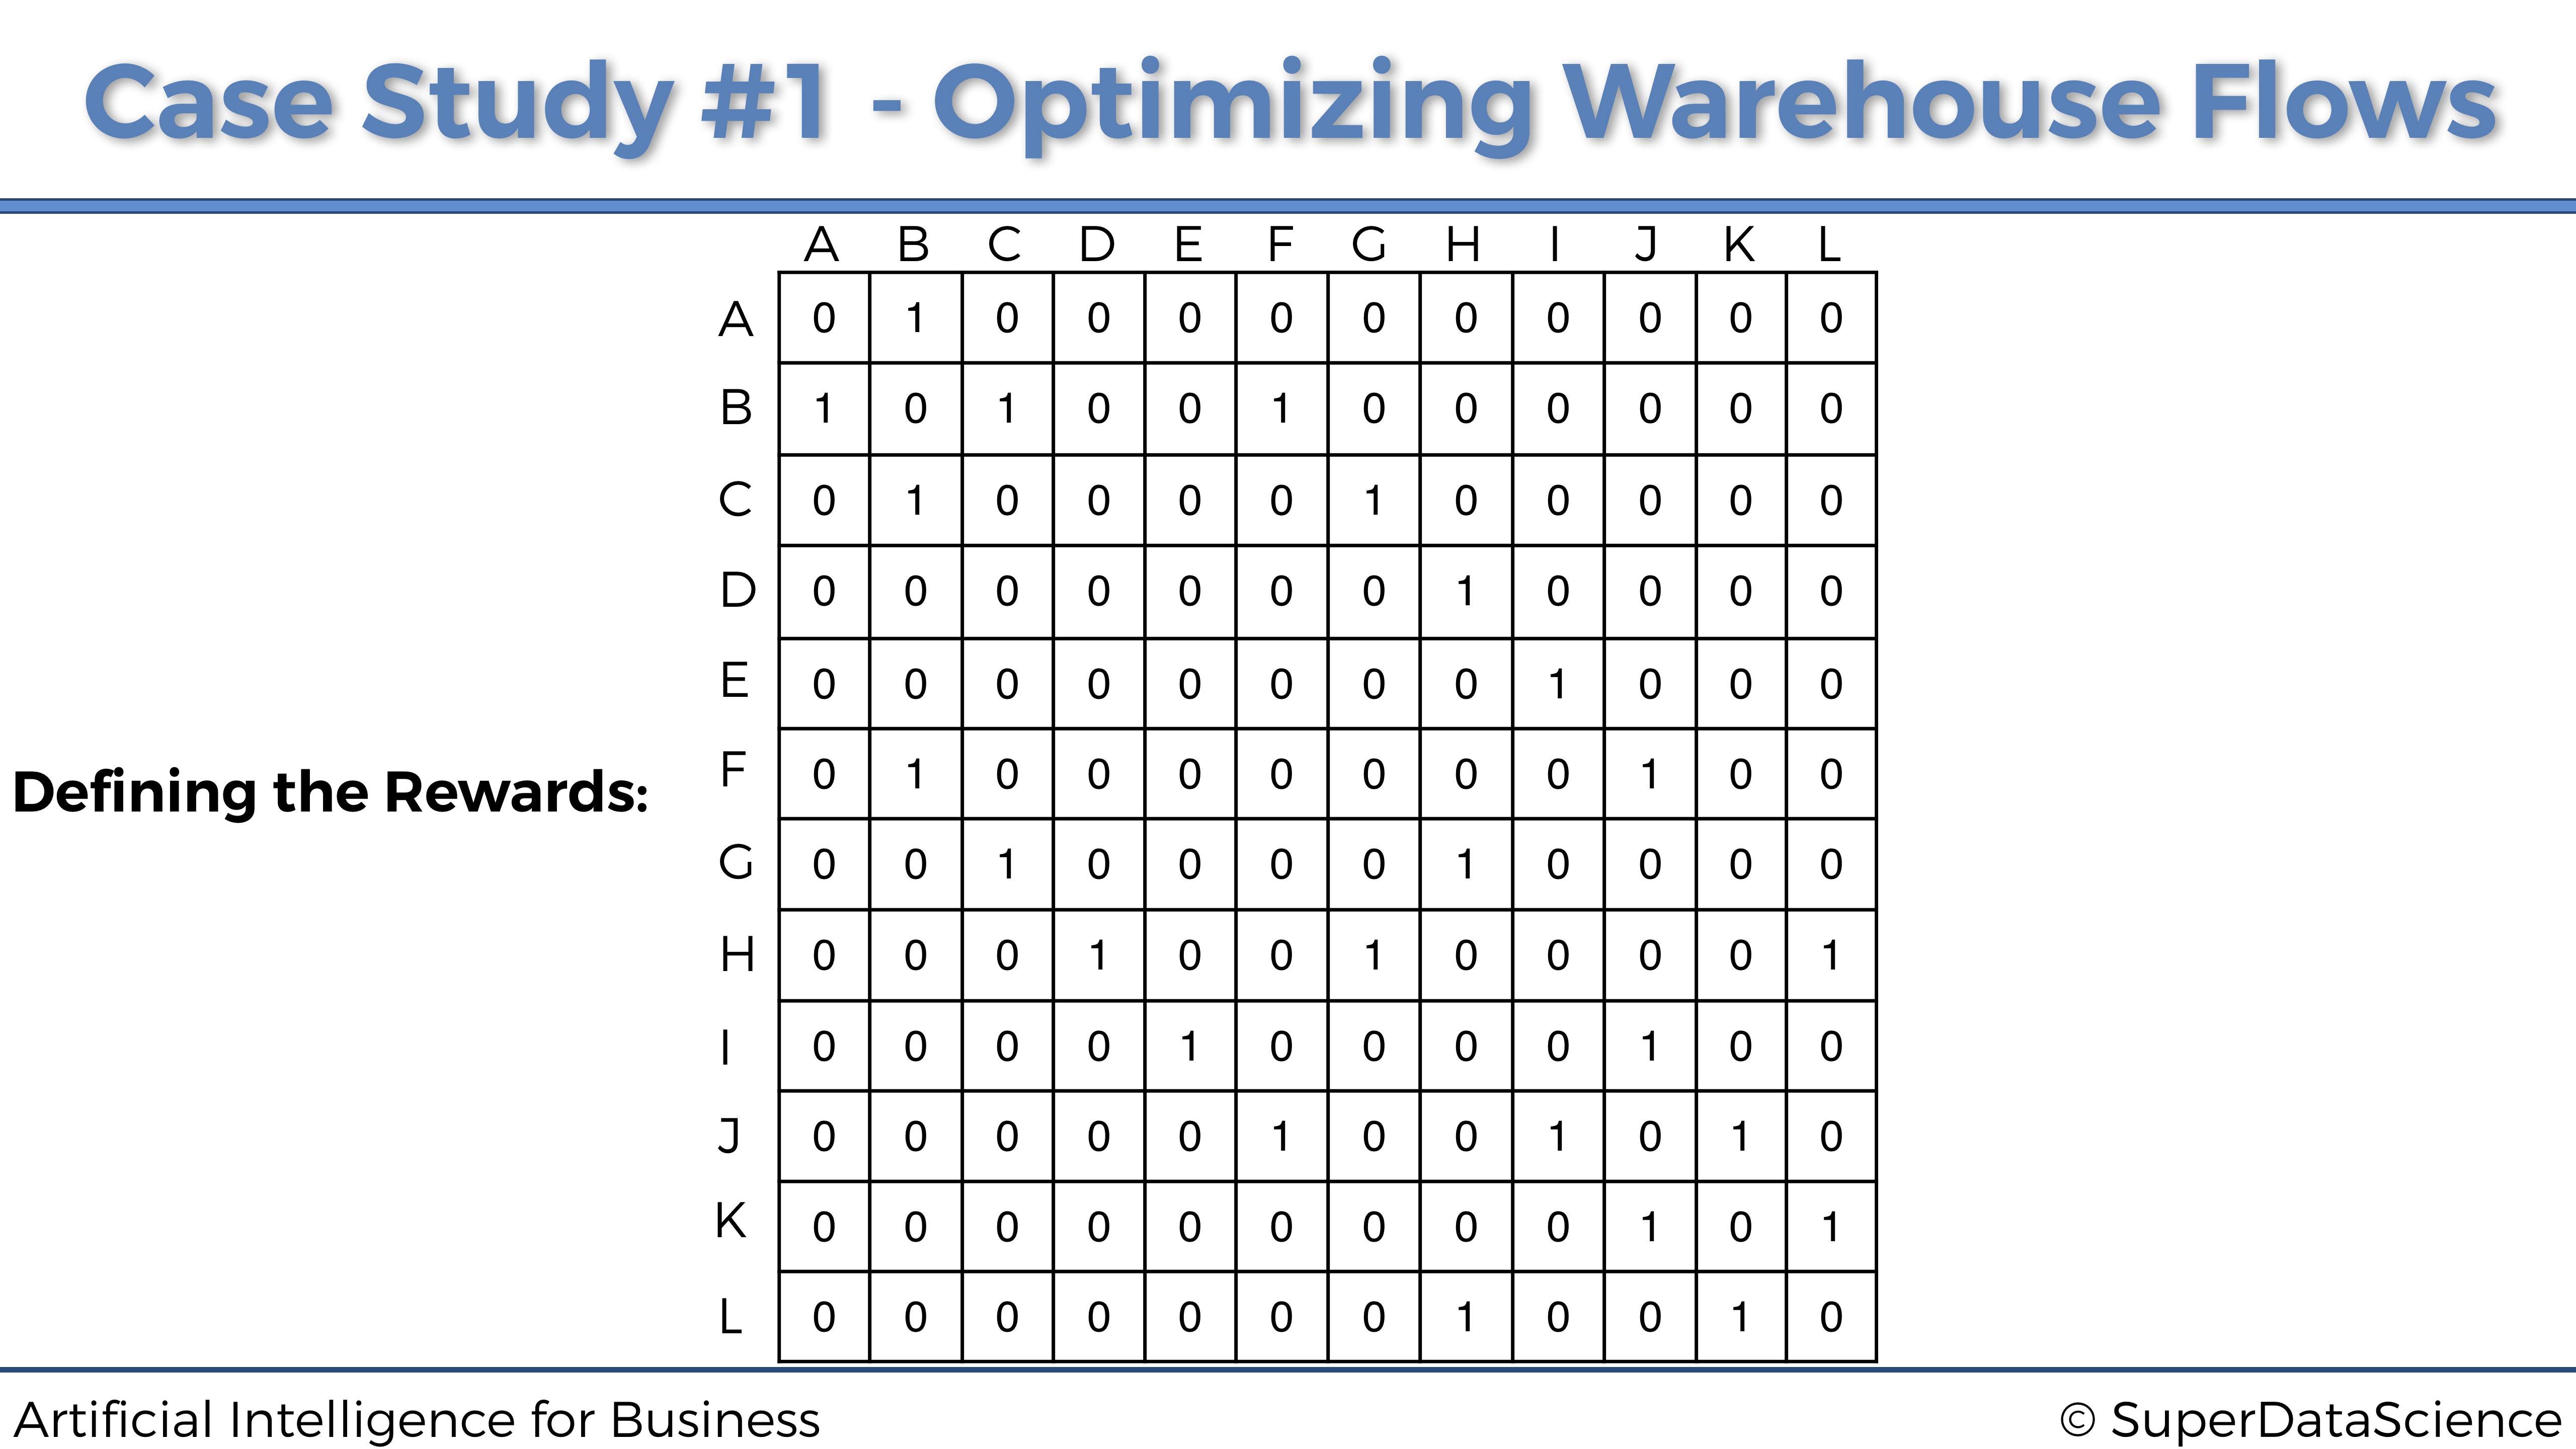
\includegraphics{Images/Rewards_Matrix_4.png}

Felicidades, acabamos de definir las recompensas. Lo hicimos simplemente construyendo esta matriz de recompensas. Es importante entender que esta es la forma en que definimos el sistema de recompensas cuando hacemos Q-Learning con un número finito de entradas y acciones. En el Caso Práctico 2, veremos que procederemos de manera muy diferente.

Ya casi hemos terminado, lo único que tenemos que hacer es atribuir grandes recompensas a las ubicaciones de mayor prioridad. Esto lo hará el sistema informático que devuelve las prioridades de recolección de productos para cada una de las 12 ubicaciones. Por lo tanto, dado que la ubicación G es la máxima prioridad, el sistema informático actualizará la matriz de recompensas atribuyendo una alta recompensa en la celda \((G, G)\):

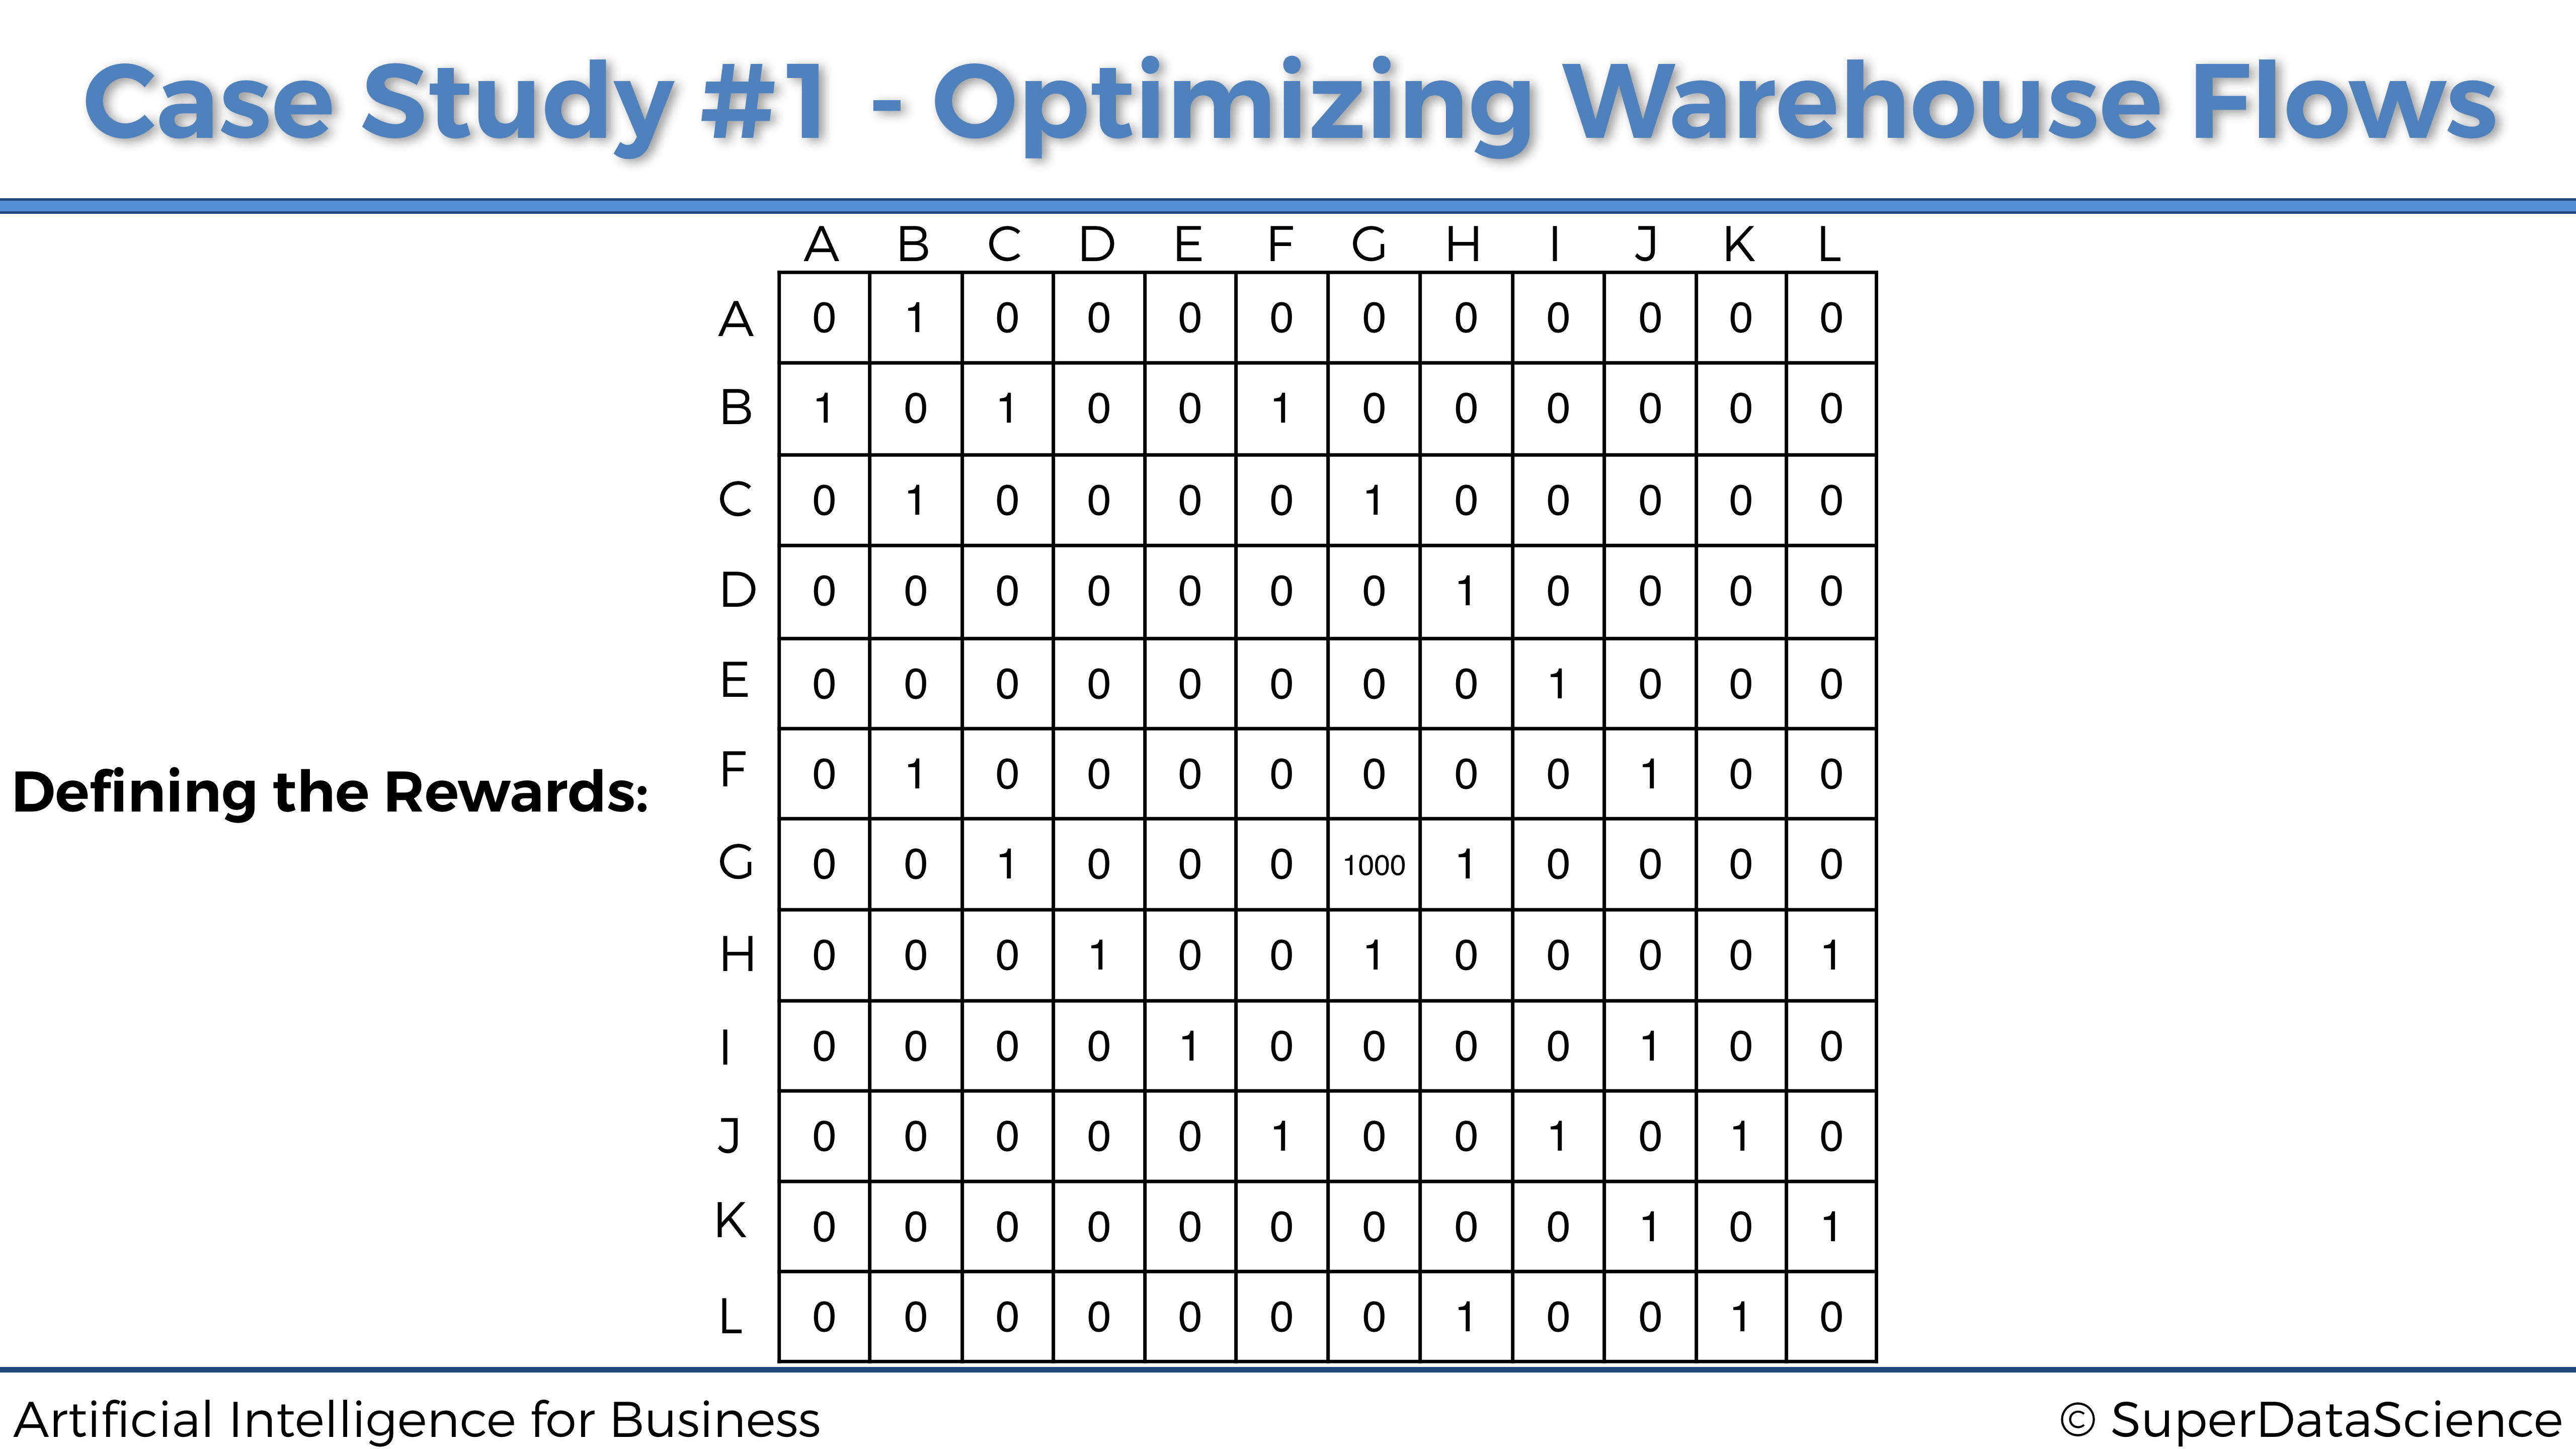
\includegraphics{Images/Rewards_Matrix_5.png}

Y así es como el sistema de recompensas funcionará con Q-Learning. Atribuimos la recompensa más alta (aquí 1000) a la ubicación de máxima prioridad G. Luego puedes ver en las clases de vídeo del curso cómo podemos atribuir una recompensa más alta a la segunda ubicación de mayor prioridad (ubicación K), para hacer que nuestro robot pase por esto ubicación intermedia de máxima prioridad, optimizando así los flujos de movimiento por el almacén.

\hypertarget{soluciuxf3n-de-inteligencia-artificial}{%
\section{Solución de Inteligencia Artificial}\label{soluciuxf3n-de-inteligencia-artificial}}

The AI Solution that will solve the problem described above is a Q-Learning model. Since the latter is based on Markov Decision Processes, or MDPs, we will start by explaining what they are, and then we will move on to the intuition and maths details behind the Q-Learning model.

\hypertarget{proceso-de-decisiuxf3n-de-markov}{%
\subsection{Proceso de Decisión de Markov}\label{proceso-de-decisiuxf3n-de-markov}}

Un Proceso de Decisión de Markov es una tupla \((S, A, T, R)\) donde:

\begin{itemize}
\tightlist
\item
  \(S\) es el conjunto de los diferentes estados. Por lo tanto, en nuestro caso de estudio: \[S = \{0,1,2,3,4,5,6,7,8,9,10,11\}\]
\item
  \(A\) es el conjunto de las diferentes acciones que se pueden llevar a cabo en cada momento \(t\). Por lo tanto, en nuestro caso de estudio: \[A = \{0,1,2,3,4,5,6,7,8,9,10,11\}\]
\item
  \(T\) es la llamada regla de transición:
\end{itemize}

\[T : (s_t \in S, s_{t+1} \in S, a_t \in A) \mapsto \mathbb{P}(s_{t+1}|s_t,a_t)\]

donde \(\mathbb {P} (s_{t + 1} | s_t, a_t)\) es la probabilidad de alcanzar el estado futuro \(s_{t + 1}\) cuando se lleva a cabo la acción \(a_t\) en el estado \(s_t\). Por lo tanto, \(T\) es la distribución de probabilidad de los estados futuros en el tiempo \(t + 1\) dado el estado actual y la acción ejecutada en el tiempo \(t\). En consecuencia, podemos predecir el estado futuro \(s_{t + 1}\) tomando un valor aleatorio de esa distribución \(T\):

\[s_{t+1} \sim T(s_t,.,a_t)\]

En nuestro estudio de caso, verás a través de nuestra implementación que esta distribución \(T\) de nuestra IA simplemente será la distribución uniforme, que es una opción clásica de distribución que funciona muy bien en el marco del Q-Learning.

\begin{itemize}
\tightlist
\item
  \(R\) es la función de recompensas:
\end{itemize}

\[R : (s_t \in S, a_t \in A) \mapsto r_t \in \mathbb{R}\]

donde \(r_t\) es la recompensa obtenida después de ejecutar la acción \(a_t\) en el estado \(s_t\). En nuestro caso práctico, esta función de recompensa es exactamente la matriz que definimos previamente.

Después de definir el proceso de decisión de Markov, ahora es importante recordar que se basa en el siguiente supuesto: la probabilidad del estado futuro \(s_{t + 1}\) solamente depende del estado actual \(s_t\) y la acción ejecutada \(a_t\), y bajo ningun concepto no depende de ninguno de los estados y acciones anteriores. Es decir:

\[\mathbb{P}(s_{t+1}|s_0,a_0,s_1,a_1,...,s_t,a_t) = \mathbb{P}(s_{t+1}|s_t,a_t)\]

En otras palabras, un proceso de decisión de Markov no tiene memoria.

\newpage

Ahora repasemos lo que va a ocurrir en términos de un proceso de decisión de Markov. En cada instante \(t\):

\begin{itemize}
\tightlist
\item
  La IA observa el estado actual \(s_t\).
\item
  La IA ejecuta la acción \(a_t\).
\item
  La IA recibe la recompensa \(r_t = R(s_t, a_t)\).
\item
  La IA entra en el siguiente estado \(s_{t+1}\).
\end{itemize}

Así que la pregunta clave es:

\begin{quote}
\textbf{¿Cómo sabe la IA qué acción llevar a cabo en cada instante \(t\)?}
\end{quote}

Para responder a esta pregunta, necesitamos introducir la función de política. La función de política \(\pi\) es exactamente la función que, dado un estado \(s_t\), devuelve la acción \(a_t\):

\[\pi: s_t \in S \mapsto a_t \in A\]

Denotemos por \(\Pi\) el conjunto de todas las funciones de política posibles. Entonces, la elección de las mejores acciones para jugar se convierte en un problema de optimización. De hecho, se trata de encontrar la política óptima \(\pi^*\) que maximice la recompensa acumulada:

\[\pi^* = \underset{\pi \in \Pi}{\textrm{argmax}} \sum_{t \ge 0} R(s_t,\pi(s_t))\]

Por lo tanto, la pregunta anterior se convierte en:

\begin{quote}
\textbf{¿Cómo encontrar esta política óptima \(\pi^*\)?}
\end{quote}

Aquí es donde entra en juego el Q-Learning.

\hypertarget{q-learning}{%
\subsection{Q-Learning}\label{q-learning}}

Antes de comenzar a entrar en los detalles de Q-Learning, necesitamos explicar el concepto del valor Q.

\textbf{El valor Q}

Para cada par de estado y acción \((s, a)\), vamos a asociar un valor numérico llamado \(Q (s, a)\):

\[Q: (s \in S, a \in A) \mapsto Q(s,a) \in \mathbb{R}\]

Diremos que \(Q (s, a)\) es \emph{el valor Q de la acción \(a\) llevada a cabo en el estado \(s\)}.

Para comprender el propósito de este \emph{Valor Q}, necesitamos introducir la Diferencia Temporal.

\textbf{La Diferencia Temporal}

Al principio \(t = 0\), todos los valores Q se inicializan a 0:

\[\forall s \in S, a \in A, Q(s,a) = 0\]

Ahora supongamos que estamos en el instante \(t\), en cierto estado \(s_t\). Llevamos a cabo una acción aleatoria \(a_t\), que nos lleva al estado \(s_{t + 1}\) y obtenemos la recompensa \(R(s_t, a_t)\).

Ahora podemos presentar la diferencia temporal, que básicamente es el corazón de Q-Learning. La diferencia temporal en el tiempo \(t\), denotada por \(TD_t(s_t, a_t)\), es la diferencia entre:

\begin{itemize}
\item
  \(R(s_t,a_t) + \gamma \underset{a}{\max}(Q(s_{t+1},a))\), es decir la recompensa \(R (s_t, a_t)\) obtenida al llevar a cabo la acción \(a_t\) en el estado \(s_t\), más el valor Q de la mejor acción jugada en el estado futuro \(s_{t + 1}\), descontado por un factor \$\gamma \in [0,1] \$, llamado factor de descuento.
\item
  y \(Q(s_t, a_t)\), es decir el valor Q de la acción \(a_t\) llevada a cabo en el estado \$ s\_t \$,
\end{itemize}

que nos lleva a:

\[TD_t(s_t,a_t) = R(s_t,a_t) + \gamma \underset{a}{\max}(Q(s_{t+1},a)) - Q(s_t,a_t)\]

\begin{quote}
\textbf{Bien, genial, pero ¿cuál es exactamente el propósito de esta diferencia temporal \(TD_t(s_t,a_t)\)?}
\end{quote}

Respondamos esta pregunta para darnos una mejor idea de la IA. \(TD_t (s_t, a_t)\) es como una recompensa intrínseca. La IA aprenderá los valores Q de tal manera que:

\begin{itemize}
\tightlist
\item
  Si \(TD_t(s_t,a_t)\) es alta, la IA recibe una \emph{buena sorpresa}.
\item
  Si \(TD_t(s_t,a_t)\) es alta, la IA recibe \emph{frustración}.
\end{itemize}

En ese sentido, la IA repetirá algunas actualizaciones de los valores Q (a través de una ecuación llamada la ecuación de Bellman) hacia diferencias temporales más altas.

En consecuencia, en el siguiente paso final del algoritmo Q-Learning, usamos la diferencia temporal para reforzar los pares (estado, acción) desde el tiempo \(t-1\) hasta el tiempo \(t\), de acuerdo con la siguiente ecuación:

\[Q_t(s_t,a_t) = Q_{t-1}(s_t,a_t) + \alpha TD_t(s_t,a_t)\]

donde \(\alpha \in \mathbb{R}\) es la tasa de aprendizaje, que determina qué tan rápido va el aprendizaje de los valores Q o qué tan grandes son las actualizaciones de los mismos. Su valor suele ser un número real elegido entre 0 y 1, como por ejemplo 0.01, 0.05, 0.1 o 0.5. Cuanto menor sea su valor, más pequeñas serán las actualizaciones de los valores Q y más larga será la ejecución del algoritmo de Q-Learning. Cuanto mayor sea su valor, mayores serán las actualizaciones de los valores Q y más rápido será el algoritmo de Q-Learning.

Esta ecuación anterior es la ecuación de Bellman. Es el pilar fundamental del Q-Learning.

Con este punto de vista, los valores Q miden la acumulación de sorpresa o frustración asociada con el par de acciones y estados \((s_t, a_t)\). En el caso de recibir sorpresa, la IA se refuerza, y en el caso de recibir frustración, la IA se debilita. Por lo tanto, queremos aprender los valores Q que le darán a la IA la máxima \emph{buena sorpresa}.

En consecuencia, la decisión de qué acción ejecutar depende principalmente del valor Q \(Q(s_t, a_t)\). Si la acción \(a_t\) ejecutada en el estado \(s_t\) está asociada con un valor Q alto \(Q (s_t, a_t)\), la IA tendrá una mayor tendencia a elegir la acción \(a_t\). Por otro lado, si la acción \(a_t\) que se ha llevado a cabo en el estado \(s_t\) está asociada con un valor Q pequeño \(Q(s_t, a_t)\), la IA tendrá una tendencia menor a elegir la acción \(a_t\).

Hay varias formas de elegir la mejor acción para ejecutar en cada esstado. Primero, cuando estamos en cierto estado \(s_t\), simplemente podríamos tomar la acción \(a_t\) que maximiza el valor Q \$ Q(s\_t, a\_t)\$:

\[a_t = \underset{a}{\textrm{argmax}}(Q(s_t,a))\]

Esta solución es el método \textbf{Argmax}.

Otra gran solución, que resulta ser una solución aún mejor para problemas complejos, es el método \textbf{Softmax}.

El método Softmax consiste en considerar para cada estado \(s\) la siguiente distribución:

\[W_s: a \in A \mapsto \frac{\exp(Q(s,a))^{\tau}}{\sum_{a'}\exp(Q(s,a'))^{\tau}} \textrm{ with } \tau \ge 0\]

Luego, elegimos qué acción \(a\) llevar a cabo mediante una muestra de un valor aleatorio de esa distribución:

\[a \sim W_s(.)\]

Sin embargo, el problema que resolveremos en el Caso Práctico 1 será lo suficientemente simple como para usar el método Argmax, así que esto es lo que elegiremos.

\hypertarget{el-algoritmo-de-q-learning-al-completo}{%
\subsection{El algoritmo de Q-Learning al completo}\label{el-algoritmo-de-q-learning-al-completo}}

Resumamos los diferentes pasos de todo el proceso de Q-Learning:

\textbf{Inicialización}

Para todas las parejas de estados \(s\) y acciones \(a\), los valores Q se inicializan a 0:

\[\forall s \in S, a \in A, Q_0(s,a) = 0\]

Comenzamos en el estado inicial \(s_0\). Llevamos a cabo una acción aleatoria posible y llegamos al primer estado \(s_1\).

\textbf{Para cada instante \(t \ge 1\)}, repetiremos un cierto número de veces (1000 veces en nuestro código) lo siguiente:

\begin{enumerate}
\def\labelenumi{\arabic{enumi}.}
\tightlist
\item
  Seleccionamos un estado aleatorio \(s_t\) de nuestros 12 estados posibles:
\end{enumerate}

\[s_t = \textrm{random}(0,1,2,3,4,5,6,7,8,9,10,11)\]

\begin{enumerate}
\def\labelenumi{\arabic{enumi}.}
\setcounter{enumi}{1}
\tightlist
\item
  Llevamos a cabo una acción aleatoria \(a_t\) que puede conducir al siguiente estado posible, es decir, de modo que \(R(s_t,a_t) > 0\):
\end{enumerate}

\[a_t = \textrm{random}(0,1,2,3,4,5,6,7,8,9,10,11) \textrm{ t.q. } R(s_t,a_t) > 0\]

\begin{enumerate}
\def\labelenumi{\arabic{enumi}.}
\setcounter{enumi}{2}
\item
  Llegamos al siguiente estado \(s_{t + 1}\) y obtenemos la recompensa \(R(s_t,a_t)\)
\item
  Calculamos la Diferencia Temporal \(TD_t(s_t,a_t)\):
\end{enumerate}

\[TD_t(s_t,a_t) = R(s_t,a_t) + \gamma \underset{a}{\max}(Q(s_{t+1},a)) - Q(s_t, a_t)\]

\begin{enumerate}
\def\labelenumi{\arabic{enumi}.}
\setcounter{enumi}{4}
\tightlist
\item
  Actualizamos el valor Q aplicando la ecuación de Bellman:
\end{enumerate}

\[Q_t(s_t,a_t) = Q_{t-1}(s_t,a_t) + \alpha TD_t(s_t,a_t)\]

\hypertarget{implementaciuxf3n}{%
\section{Implementación}\label{implementaciuxf3n}}

Ahora proporcionemos y expliquemos la implementación completa de este modelo de Q-Learning, la solución de nuestro problema de optimización de flujos de almacén.

Primero, comenzamos importando las librerías que se usarán en esta implementación. Estos solo incluyen la biblioteca \texttt{numpy}, que ofrece una forma práctica de trabajar con matrices y operaciones matemáticas:

\begin{Shaded}
\begin{Highlighting}[]
\CommentTok{# Importar las librerías}
\ImportTok{import}\NormalTok{ numpy }\ImportTok{as}\NormalTok{ np}
\end{Highlighting}
\end{Shaded}

Luego establecemos los parámetros de nuestro modelo. Estos incluyen el factor de descuento \(\gamma\) y la tasa de aprendizaje \$\alpha \$, que como vimos en la Sección 1.2, son los únicos parámetros del algoritmo Q-Learning:

\begin{Shaded}
\begin{Highlighting}[]
\CommentTok{# Configuración de los parámetros gamma y alfa para el Q-Learning}
\NormalTok{gamma }\OperatorTok{=} \FloatTok{0.75}
\NormalTok{alpha }\OperatorTok{=} \FloatTok{0.9}
\end{Highlighting}
\end{Shaded}

Las dos secciones de código anteriores eran simplemente las secciones introductorias, antes de comenzar realmente a construir nuestro modelo de IA. Ahora el siguiente paso es comenzar la primera parte de nuestra implementación: Parte 1 - Definición del entorno. Y para eso, por supuesto, comenzamos definiendo los estados, con un diccionario que asigna los nombres de las ubicaciones (en letras de la A a la L) en los estados (en índices del 0 al 11):

\begin{Shaded}
\begin{Highlighting}[]
\CommentTok{# PARTE 1 - DEFINICIÓN DEL ENTORNO}

\CommentTok{# Definición de los estados}
\NormalTok{location_to_state }\OperatorTok{=}\NormalTok{ \{}\StringTok{'A'}\NormalTok{: }\DecValTok{0}\NormalTok{,}
                     \StringTok{'B'}\NormalTok{: }\DecValTok{1}\NormalTok{,}
                     \StringTok{'C'}\NormalTok{: }\DecValTok{2}\NormalTok{,}
                     \StringTok{'D'}\NormalTok{: }\DecValTok{3}\NormalTok{,}
                     \StringTok{'E'}\NormalTok{: }\DecValTok{4}\NormalTok{,}
                     \StringTok{'F'}\NormalTok{: }\DecValTok{5}\NormalTok{,}
                     \StringTok{'G'}\NormalTok{: }\DecValTok{6}\NormalTok{,}
                     \StringTok{'H'}\NormalTok{: }\DecValTok{7}\NormalTok{,}
                     \StringTok{'I'}\NormalTok{: }\DecValTok{8}\NormalTok{,}
                     \StringTok{'J'}\NormalTok{: }\DecValTok{9}\NormalTok{,}
                     \StringTok{'K'}\NormalTok{: }\DecValTok{10}\NormalTok{,}
                     \StringTok{'L'}\NormalTok{: }\DecValTok{11}\NormalTok{\}}
\end{Highlighting}
\end{Shaded}

Luego definimos las acciones, con una simple lista de índices del 0 al 11. Recuerda que cada índice de acción corresponde al siguiente estado (siguiente ubicación) al que conduce dicha acción:

\begin{Shaded}
\begin{Highlighting}[]
\CommentTok{# Definición de las acciones}
\NormalTok{actions }\OperatorTok{=}\NormalTok{ [}\DecValTok{0}\NormalTok{,}\DecValTok{1}\NormalTok{,}\DecValTok{2}\NormalTok{,}\DecValTok{3}\NormalTok{,}\DecValTok{4}\NormalTok{,}\DecValTok{5}\NormalTok{,}\DecValTok{6}\NormalTok{,}\DecValTok{7}\NormalTok{,}\DecValTok{8}\NormalTok{,}\DecValTok{9}\NormalTok{,}\DecValTok{10}\NormalTok{,}\DecValTok{11}\NormalTok{]}
\end{Highlighting}
\end{Shaded}

Y eventualmente, definimos las recompensas, creando una matriz de recompensas, donde las filas corresponden a los estados actuales \(s_t\), las columnas corresponden a las acciones \(a_t\) que conducen al siguiente estado \(s_{t + 1}\), y las celdas contienen las recompensas \(R(s_t, a_t)\). Si una celda \((s_t, a_t)\) tiene un 1, eso significa que podemos llevar a cabo la acción \(a_t\) del estado actual \(s_t\) para llegar al siguiente estado \(s_{t + 1}\). Si una celda \((s_t, a_t)\) tiene un 0, eso significa que no podemos llevar a cabo la acción \(a_t\) del estado actual \(s_t\) para llegar a cualquier estado siguiente \(s_{t + 1}\). Y por ahora colocaremos manualmente una alta recompensa (1000) dentro de la celda correspondiente a la ubicación G, porque es la ubicación de máxima prioridad donde el almacén autónomo tiene que ir a recoger los productos. Como la ubicación G ha codificado el estado como índice 6, colocamos una recompensa de 1000 en la celda de la fila 6 y la columna 6. Luego, mejoraremos nuestra solución al implementar una forma automática de ir a la ubicación de máxima prioridad, sin tener que actualizar manualmente la matriz de recompensas y dejándola inicializada con 0s y 1s como debería ser. Pero mientras tanto, aquí está debajo de nuestra matriz de recompensas, incluida la actualización manual:

\begin{Shaded}
\begin{Highlighting}[]
\CommentTok{# Definición de las recompensas}
\NormalTok{R }\OperatorTok{=}\NormalTok{ np.array([[}\DecValTok{0}\NormalTok{,}\DecValTok{1}\NormalTok{,}\DecValTok{0}\NormalTok{,}\DecValTok{0}\NormalTok{,}\DecValTok{0}\NormalTok{,}\DecValTok{0}\NormalTok{,}\DecValTok{0}\NormalTok{,}\DecValTok{0}\NormalTok{,}\DecValTok{0}\NormalTok{,}\DecValTok{0}\NormalTok{,}\DecValTok{0}\NormalTok{,}\DecValTok{0}\NormalTok{],}
\NormalTok{              [}\DecValTok{1}\NormalTok{,}\DecValTok{0}\NormalTok{,}\DecValTok{1}\NormalTok{,}\DecValTok{0}\NormalTok{,}\DecValTok{0}\NormalTok{,}\DecValTok{1}\NormalTok{,}\DecValTok{0}\NormalTok{,}\DecValTok{0}\NormalTok{,}\DecValTok{0}\NormalTok{,}\DecValTok{0}\NormalTok{,}\DecValTok{0}\NormalTok{,}\DecValTok{0}\NormalTok{],}
\NormalTok{              [}\DecValTok{0}\NormalTok{,}\DecValTok{1}\NormalTok{,}\DecValTok{0}\NormalTok{,}\DecValTok{0}\NormalTok{,}\DecValTok{0}\NormalTok{,}\DecValTok{0}\NormalTok{,}\DecValTok{1}\NormalTok{,}\DecValTok{0}\NormalTok{,}\DecValTok{0}\NormalTok{,}\DecValTok{0}\NormalTok{,}\DecValTok{0}\NormalTok{,}\DecValTok{0}\NormalTok{],}
\NormalTok{              [}\DecValTok{0}\NormalTok{,}\DecValTok{0}\NormalTok{,}\DecValTok{0}\NormalTok{,}\DecValTok{0}\NormalTok{,}\DecValTok{0}\NormalTok{,}\DecValTok{0}\NormalTok{,}\DecValTok{0}\NormalTok{,}\DecValTok{1}\NormalTok{,}\DecValTok{0}\NormalTok{,}\DecValTok{0}\NormalTok{,}\DecValTok{0}\NormalTok{,}\DecValTok{0}\NormalTok{],}
\NormalTok{              [}\DecValTok{0}\NormalTok{,}\DecValTok{0}\NormalTok{,}\DecValTok{0}\NormalTok{,}\DecValTok{0}\NormalTok{,}\DecValTok{0}\NormalTok{,}\DecValTok{0}\NormalTok{,}\DecValTok{0}\NormalTok{,}\DecValTok{0}\NormalTok{,}\DecValTok{1}\NormalTok{,}\DecValTok{0}\NormalTok{,}\DecValTok{0}\NormalTok{,}\DecValTok{0}\NormalTok{],}
\NormalTok{              [}\DecValTok{0}\NormalTok{,}\DecValTok{1}\NormalTok{,}\DecValTok{0}\NormalTok{,}\DecValTok{0}\NormalTok{,}\DecValTok{0}\NormalTok{,}\DecValTok{0}\NormalTok{,}\DecValTok{0}\NormalTok{,}\DecValTok{0}\NormalTok{,}\DecValTok{0}\NormalTok{,}\DecValTok{1}\NormalTok{,}\DecValTok{0}\NormalTok{,}\DecValTok{0}\NormalTok{],}
\NormalTok{              [}\DecValTok{0}\NormalTok{,}\DecValTok{0}\NormalTok{,}\DecValTok{1}\NormalTok{,}\DecValTok{0}\NormalTok{,}\DecValTok{0}\NormalTok{,}\DecValTok{0}\NormalTok{,}\DecValTok{1000}\NormalTok{,}\DecValTok{1}\NormalTok{,}\DecValTok{0}\NormalTok{,}\DecValTok{0}\NormalTok{,}\DecValTok{0}\NormalTok{,}\DecValTok{0}\NormalTok{],}
\NormalTok{              [}\DecValTok{0}\NormalTok{,}\DecValTok{0}\NormalTok{,}\DecValTok{0}\NormalTok{,}\DecValTok{1}\NormalTok{,}\DecValTok{0}\NormalTok{,}\DecValTok{0}\NormalTok{,}\DecValTok{1}\NormalTok{,}\DecValTok{0}\NormalTok{,}\DecValTok{0}\NormalTok{,}\DecValTok{0}\NormalTok{,}\DecValTok{0}\NormalTok{,}\DecValTok{1}\NormalTok{],}
\NormalTok{              [}\DecValTok{0}\NormalTok{,}\DecValTok{0}\NormalTok{,}\DecValTok{0}\NormalTok{,}\DecValTok{0}\NormalTok{,}\DecValTok{1}\NormalTok{,}\DecValTok{0}\NormalTok{,}\DecValTok{0}\NormalTok{,}\DecValTok{0}\NormalTok{,}\DecValTok{0}\NormalTok{,}\DecValTok{1}\NormalTok{,}\DecValTok{0}\NormalTok{,}\DecValTok{0}\NormalTok{],}
\NormalTok{              [}\DecValTok{0}\NormalTok{,}\DecValTok{0}\NormalTok{,}\DecValTok{0}\NormalTok{,}\DecValTok{0}\NormalTok{,}\DecValTok{0}\NormalTok{,}\DecValTok{1}\NormalTok{,}\DecValTok{0}\NormalTok{,}\DecValTok{0}\NormalTok{,}\DecValTok{1}\NormalTok{,}\DecValTok{0}\NormalTok{,}\DecValTok{1}\NormalTok{,}\DecValTok{0}\NormalTok{],}
\NormalTok{              [}\DecValTok{0}\NormalTok{,}\DecValTok{0}\NormalTok{,}\DecValTok{0}\NormalTok{,}\DecValTok{0}\NormalTok{,}\DecValTok{0}\NormalTok{,}\DecValTok{0}\NormalTok{,}\DecValTok{0}\NormalTok{,}\DecValTok{0}\NormalTok{,}\DecValTok{0}\NormalTok{,}\DecValTok{1}\NormalTok{,}\DecValTok{0}\NormalTok{,}\DecValTok{1}\NormalTok{],}
\NormalTok{              [}\DecValTok{0}\NormalTok{,}\DecValTok{0}\NormalTok{,}\DecValTok{0}\NormalTok{,}\DecValTok{0}\NormalTok{,}\DecValTok{0}\NormalTok{,}\DecValTok{0}\NormalTok{,}\DecValTok{0}\NormalTok{,}\DecValTok{1}\NormalTok{,}\DecValTok{0}\NormalTok{,}\DecValTok{0}\NormalTok{,}\DecValTok{1}\NormalTok{,}\DecValTok{0}\NormalTok{]])}
\end{Highlighting}
\end{Shaded}

Eso finaliza esta primera parte. Ahora comencemos la segunda parte de nuestra implementación: Parte 2 - Construcción la solución de IA con Q-Learning. En ese sentido, vamos a seguir el algoritmo de Q-Learning exactamente como lo vimos en la Sección 1.2. Por lo tanto, primero inicializamos todos los valores Q, creando nuestra matriz de valores Q llena de ceros (en los cuales, las filas corresponden a los estados actuales \(s_t\), las columnas corresponden a las acciones \(a_t\) que conducen al siguiente estado \$s\_\{t + 1\} \$, y las celdas contienen los valores Q, \$Q (s\_t, a\_t)) \$:

\begin{Shaded}
\begin{Highlighting}[]
\CommentTok{# PARTE 2 - CONSTRUCCIÓN DE LA SOLUCIÓN DE IA CON Q-LEARNING}

\CommentTok{# Inicialización de los valores Q}
\NormalTok{Q }\OperatorTok{=}\NormalTok{ np.array(np.zeros([}\DecValTok{12}\NormalTok{,}\DecValTok{12}\NormalTok{]))}
\end{Highlighting}
\end{Shaded}

Luego, por supuesto, implementamos el proceso de Q-Learning, con un bucle \texttt{for} que llevará a cabo un total de 1000 iteraciones, repitiendo 1000 veces los pasos del proceso de Q-Learning que analizamos a fondo al final de la Sección 1.2:

\begin{Shaded}
\begin{Highlighting}[]
\CommentTok{# Implementación del proceso de Q-Learning}
\ControlFlowTok{for}\NormalTok{ i }\KeywordTok{in} \BuiltInTok{range}\NormalTok{(}\DecValTok{1000}\NormalTok{):}
\NormalTok{    current_state }\OperatorTok{=}\NormalTok{ np.random.randint(}\DecValTok{0}\NormalTok{,}\DecValTok{12}\NormalTok{)}
\NormalTok{    playable_actions }\OperatorTok{=}\NormalTok{ []}
    \ControlFlowTok{for}\NormalTok{ j }\KeywordTok{in} \BuiltInTok{range}\NormalTok{(}\DecValTok{12}\NormalTok{):}
        \ControlFlowTok{if}\NormalTok{ R[current_state, j] }\OperatorTok{>} \DecValTok{0}\NormalTok{:}
\NormalTok{            playable_actions.append(j)}
\NormalTok{    next_state }\OperatorTok{=}\NormalTok{ np.random.choice(playable_actions)}
\NormalTok{    TD }\OperatorTok{=}\NormalTok{ R[current_state, next_state] }\OperatorTok{+}\NormalTok{ gamma}\OperatorTok{*}\NormalTok{Q[next_state, np.argmax(Q[next_state,])]}
         \OperatorTok{-}\NormalTok{ Q[current_state, next_state]}
\NormalTok{    Q[current_state, next_state] }\OperatorTok{=}\NormalTok{ Q[current_state, next_state] }\OperatorTok{+}\NormalTok{ alpha}\OperatorTok{*}\NormalTok{TD}
\end{Highlighting}
\end{Shaded}

Opcional: en esta etapa del código, nuestra matriz de valores Q está lista. Podemos echarle un vistazo ejecutando todo el código que hemos implementado hasta ahora e ingresando las siguientes dos instrucciones en la consola:

\begin{Shaded}
\begin{Highlighting}[]
\BuiltInTok{print}\NormalTok{(}\StringTok{"Q-Values:"}\NormalTok{)}
\BuiltInTok{print}\NormalTok{(Q.astype(}\BuiltInTok{int}\NormalTok{))}
\end{Highlighting}
\end{Shaded}

Y obtenemos la siguiente matriz de valores Q finales:

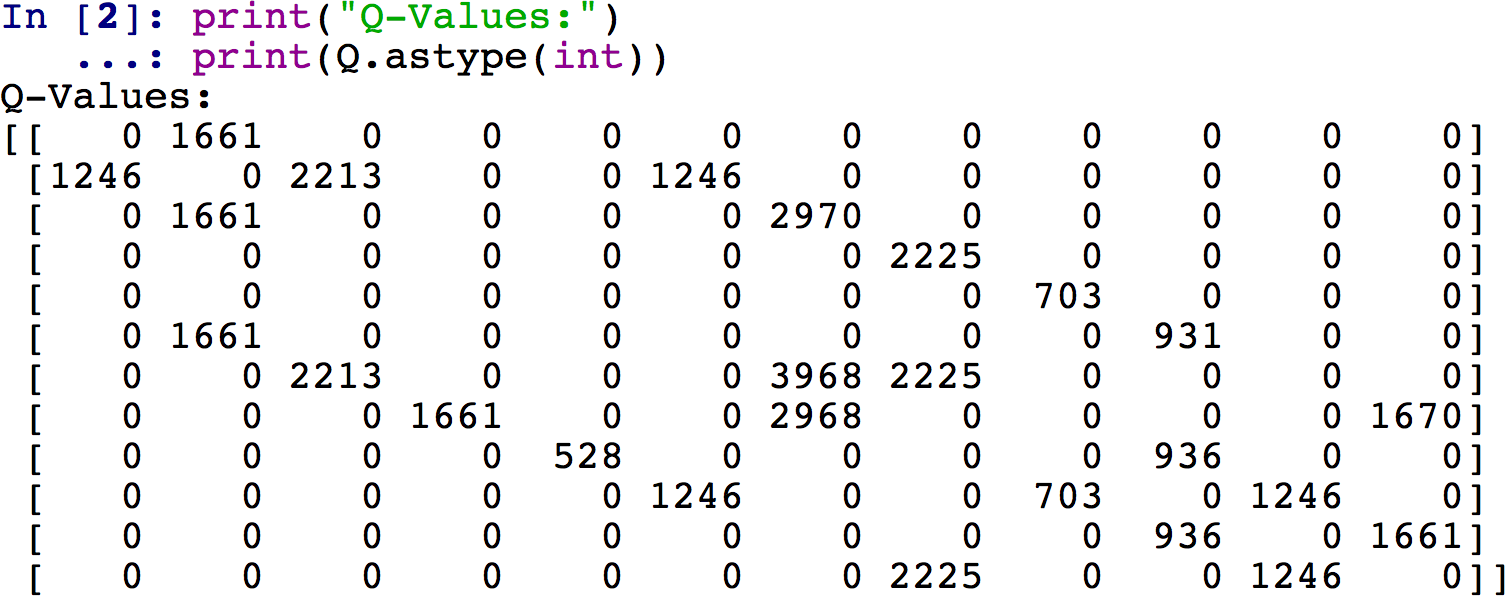
\includegraphics{Images/Q_Values_Console.png}

Para una mayor claridad visual, incluso puede verificarse la matriz de valores Q directamente en el Explorador de variables, haciendo doble clic en la variable Q. Luego, para obtener los valores Q como enteros, es conveniente hacer clic en \texttt{Formato} e ingresar un formato de como floante como \texttt{\%.0f}. Se obtiene en este caso el siguiente resultado, que es un poco más claro ya que se pueden ver en la matriz Q los índices de las filas y columnas de la misma:

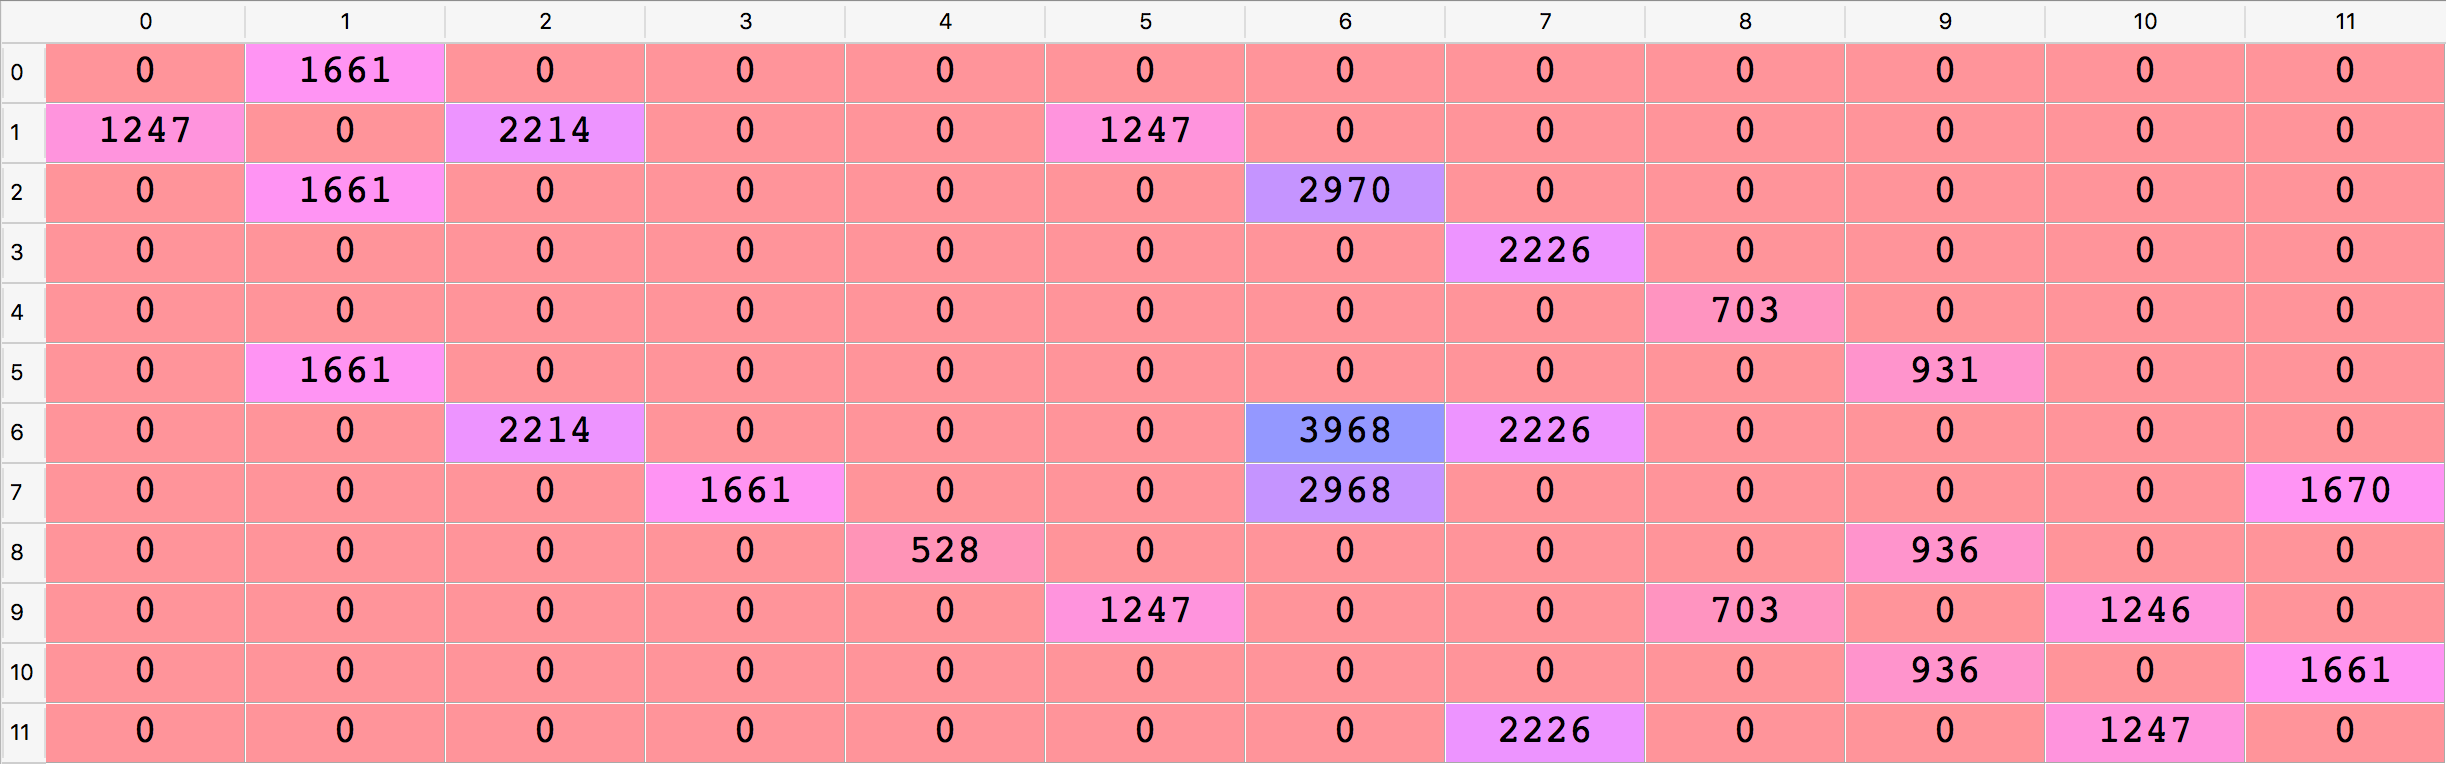
\includegraphics{Images/Q_Values_Variable_Explorer.png}

Bien, ahora que tenemos nuestra matriz de valores Q, ¡estamos listos para llevarlo a producción! Por lo tanto, podemos pasar a la tercera parte de la implementación, Parte 3: Poner el modelo en producción, dentro de la cual calcularemos la ruta óptima desde cualquier ubicación inicial a cualquier ubicación final de máxima prioridad. La idea aquí será implementar una función de \emph{ruta}, que tomará como entradas la ubicación de inicio donde se encuentra nuestro robot de almacén autónomo en un momento específico y la ubicación de finalización donde tiene que ir con la máxima prioridad, y eso volverá como genera la ruta más corta dentro de una lista. Sin embargo, dado que queremos indicar las ubicaciones con sus nombres (en letras), a diferencia de sus estados (en índices), necesitaremos un diccionario que asigne los estados de ubicaciones (en índices) a los nombres de ubicaciones (en letras). Y eso es lo primero que haremos aquí en esta tercera parte, usando un truco para invertir nuestro diccionario anterior \texttt{location\textbackslash{}\_to\textbackslash{}\_state}, ya que de hecho simplemente queremos obtener el mapeo inverso exacto de este diccionario:

\begin{Shaded}
\begin{Highlighting}[]
\CommentTok{# PARTE 3 - PONER EL MODELO EN PRODUCCIÓN}

\CommentTok{# Hacer un mapeo de los estados a las ubicaciones}
\NormalTok{state_to_location }\OperatorTok{=}\NormalTok{ \{state: location }\ControlFlowTok{for}\NormalTok{ location, state }\KeywordTok{in}\NormalTok{ location_to_state.items()\}}
\end{Highlighting}
\end{Shaded}

Aquí es cuando entra en juego la sección de código más importante. Estamos a punto de implementar la función final \texttt{route\ ()} que tomará como entradas las ubicaciones de inicio y finalización, y que devolverá la ruta óptima entre estas dos ubicaciones. Para explicar exactamente qué hará esta función de ruta, enumeremos los diferentes pasos del proceso, al pasar de la ubicación E a la ubicación G:

\begin{enumerate}
\def\labelenumi{\arabic{enumi}.}
\tightlist
\item
  Comenzamos en nuestra ubicación inicial E.
\item
  Obtenemos el estado de ubicación E, que según nuestro mapeo \texttt{location\_to\_state} es \(s_0 = 4\).
\item
  En la fila del estado \(s_0 = 4\) de nuestra matriz de valores Q, hallamos la columna con el mayor valor Q (703).
\item
  Esta columna tiene el índice 8, por lo que ejecutamos la acción del índice 8 que nos lleva al siguiente estado \(s_{t+1} = 8\).
\item
  Obtenemos la ubicación del estado 8, que según nuestro mapeo \texttt{state\_to\_location} es la ubicación I. Por lo tanto, nuestra próxima ubicación es la ubicación I, que se adjunta a nuestra lista que contiene la ruta óptima global.
\item
  Repetimos los mismos 5 pasos anteriores desde nuestra nueva ubicación inicial I, hasta llegar a nuestro destino final, la ubicación G.
\end{enumerate}

Por lo tanto, dado que no sabemos cuántas ubicaciones tendremos que atravesar entre las ubicaciones inicial y final, tenemos que hacer un bucle \texttt{while} que repetirá el proceso de 5 pasos descrito anteriormente, y que se detendrá tan pronto como lo hagamos llegar a la ubicación final de máxima prioridad:

\begin{Shaded}
\begin{Highlighting}[]
\CommentTok{# Hacer la función final que devolverá la ruta óptima}
\KeywordTok{def}\NormalTok{ route(starting_location, ending_location):}
\NormalTok{    route }\OperatorTok{=}\NormalTok{ [starting_location]}
\NormalTok{    next_location }\OperatorTok{=}\NormalTok{ starting_location}
    \ControlFlowTok{while}\NormalTok{ (next_location }\OperatorTok{!=}\NormalTok{ ending_location):}
\NormalTok{        starting_state }\OperatorTok{=}\NormalTok{ location_to_state[starting_location]}
\NormalTok{        next_state }\OperatorTok{=}\NormalTok{ np.argmax(Q[starting_state,])}
\NormalTok{        next_location }\OperatorTok{=}\NormalTok{ state_to_location[next_state]}
\NormalTok{        route.append(next_location)}
\NormalTok{        starting_location }\OperatorTok{=}\NormalTok{ next_location}
    \ControlFlowTok{return}\NormalTok{ route}
\end{Highlighting}
\end{Shaded}

¡Felicidades, nuestra herramienta ya está lista! Cuando lo probamos para ir de E a G, obtenemos las dos rutas óptimas posibles después de imprimir la ruta final ejecutando el código completo varias veces:

\begin{Shaded}
\begin{Highlighting}[]
\CommentTok{# Imprimir la ruta final}
\BuiltInTok{print}\NormalTok{(}\StringTok{'Route:'}\NormalTok{)}
\NormalTok{route(}\StringTok{'E'}\NormalTok{, }\StringTok{'G'}\NormalTok{)}
\end{Highlighting}
\end{Shaded}

\begin{Shaded}
\begin{Highlighting}[]
\NormalTok{Route:}
\NormalTok{Out[}\DecValTok{1}\NormalTok{]: [}\StringTok{'E'}\NormalTok{, }\StringTok{'I'}\NormalTok{, }\StringTok{'J'}\NormalTok{, }\StringTok{'F'}\NormalTok{, }\StringTok{'B'}\NormalTok{, }\StringTok{'C'}\NormalTok{, }\StringTok{'G'}\NormalTok{]}
\NormalTok{Out[}\DecValTok{2}\NormalTok{]: [}\StringTok{'E'}\NormalTok{, }\StringTok{'I'}\NormalTok{, }\StringTok{'J'}\NormalTok{, }\StringTok{'K'}\NormalTok{, }\StringTok{'L'}\NormalTok{, }\StringTok{'H'}\NormalTok{, }\StringTok{'G'}\NormalTok{]}
\end{Highlighting}
\end{Shaded}

Bien, tenemos una primera versión del modelo que funciona bien. Pero podemos mejorarlo de dos maneras. Primero, al automatizar la atribución de recompensas a la ubicación de máxima prioridad, para que no tengamos que hacerlo manualmente. Y segundo, al agregar una función que nos da la opción de ir a una ubicación intermedia antes de ir a la ubicación de máxima prioridad. Esa ubicación intermedia debe estar, por supuesto, en las 3 ubicaciones prioritarias principales. Y, de hecho, en nuestra clasificación de ubicaciones de máxima prioridad, la segunda ubicación de máxima prioridad es la ubicación K. Por lo tanto, para optimizar aún más los flujos de almacén, nuestro robot de almacén autónomo debe ir por la ubicación K para recoger los productos en su camino a la ubicación de máxima prioridad G. Una forma de hacer esto es tener la opción de ir a cualquier ubicación intermedia en el proceso de nuestra función \texttt{route()}. Y esto es exactamente lo que implementaremos como segunda mejora. Pero primero, implementemos la primera mejora, que automatiza la atribución de recompensas.

La forma de hacerlo es en dos pasos: primero debemos hacer una copia (llamada \texttt{R\_new}) de nuestra matriz de recompensa dentro de la cual la función \texttt{route()} actualizará automáticamente la recompensa en la celda de la ubicación final. De hecho, la ubicación final es una de las entradas de la función \texttt{route()}, por lo que al usar nuestro diccionario de \texttt{location\_to\_state} podemos encontrar fácilmente esa celda y actualizar su recompensa a 1000. Y segundo, debemos incluir toda la lógica del algoritmo de Q-learning (incluido el paso de inicialización) dentro de la función de ruta, justo después de hacer esa actualización de la recompensa en nuestra copia de la matriz de recompensas. De hecho, en nuestra implementación anterior anterior, el proceso de Q-Learning ocurre en la versión original de la matriz de recompensas, que ahora se supone que permanece como está, es decir, se inicializa solo a 1s y 0s. Por lo tanto, debemos incluir el proceso de Q-Learning dentro de la función de ruta y hacer que suceda en nuestra copia \texttt{R\_new} de la matriz de recompensas, en lugar de la matriz de recompensas original \texttt{R}. Por lo tanto, nuestra implementación completa se convierte en lo siguiente:

\begin{Shaded}
\begin{Highlighting}[]
\CommentTok{# Inteligencia Artificial aplicada a Negocios y Empresas}

\CommentTok{# Optimización de Procesos en un almacén con Q-Learning}

\CommentTok{# # Importar las librerías}
\ImportTok{import}\NormalTok{ numpy }\ImportTok{as}\NormalTok{ np}

\CommentTok{# Configuración de los parámetros gamma y alfa para el Q-Learning}
\NormalTok{gamma }\OperatorTok{=} \FloatTok{0.75}
\NormalTok{alpha }\OperatorTok{=} \FloatTok{0.9}

\CommentTok{# PARTE 1 - DEFINICIÓN DEL ENTORNO}

\CommentTok{# Definición de los estados}
\NormalTok{location_to_state }\OperatorTok{=}\NormalTok{ \{}\StringTok{'A'}\NormalTok{: }\DecValTok{0}\NormalTok{,}
                     \StringTok{'B'}\NormalTok{: }\DecValTok{1}\NormalTok{,}
                     \StringTok{'C'}\NormalTok{: }\DecValTok{2}\NormalTok{,}
                     \StringTok{'D'}\NormalTok{: }\DecValTok{3}\NormalTok{,}
                     \StringTok{'E'}\NormalTok{: }\DecValTok{4}\NormalTok{,}
                     \StringTok{'F'}\NormalTok{: }\DecValTok{5}\NormalTok{,}
                     \StringTok{'G'}\NormalTok{: }\DecValTok{6}\NormalTok{,}
                     \StringTok{'H'}\NormalTok{: }\DecValTok{7}\NormalTok{,}
                     \StringTok{'I'}\NormalTok{: }\DecValTok{8}\NormalTok{,}
                     \StringTok{'J'}\NormalTok{: }\DecValTok{9}\NormalTok{,}
                     \StringTok{'K'}\NormalTok{: }\DecValTok{10}\NormalTok{,}
                     \StringTok{'L'}\NormalTok{: }\DecValTok{11}\NormalTok{\}}

\CommentTok{# Definición de las acciones}
\NormalTok{actions }\OperatorTok{=}\NormalTok{ [}\DecValTok{0}\NormalTok{,}\DecValTok{1}\NormalTok{,}\DecValTok{2}\NormalTok{,}\DecValTok{3}\NormalTok{,}\DecValTok{4}\NormalTok{,}\DecValTok{5}\NormalTok{,}\DecValTok{6}\NormalTok{,}\DecValTok{7}\NormalTok{,}\DecValTok{8}\NormalTok{,}\DecValTok{9}\NormalTok{,}\DecValTok{10}\NormalTok{,}\DecValTok{11}\NormalTok{]}

\CommentTok{# Definición de las recompensas}
\NormalTok{R }\OperatorTok{=}\NormalTok{ np.array([[}\DecValTok{0}\NormalTok{,}\DecValTok{1}\NormalTok{,}\DecValTok{0}\NormalTok{,}\DecValTok{0}\NormalTok{,}\DecValTok{0}\NormalTok{,}\DecValTok{0}\NormalTok{,}\DecValTok{0}\NormalTok{,}\DecValTok{0}\NormalTok{,}\DecValTok{0}\NormalTok{,}\DecValTok{0}\NormalTok{,}\DecValTok{0}\NormalTok{,}\DecValTok{0}\NormalTok{],}
\NormalTok{              [}\DecValTok{1}\NormalTok{,}\DecValTok{0}\NormalTok{,}\DecValTok{1}\NormalTok{,}\DecValTok{0}\NormalTok{,}\DecValTok{0}\NormalTok{,}\DecValTok{1}\NormalTok{,}\DecValTok{0}\NormalTok{,}\DecValTok{0}\NormalTok{,}\DecValTok{0}\NormalTok{,}\DecValTok{0}\NormalTok{,}\DecValTok{0}\NormalTok{,}\DecValTok{0}\NormalTok{],}
\NormalTok{              [}\DecValTok{0}\NormalTok{,}\DecValTok{1}\NormalTok{,}\DecValTok{0}\NormalTok{,}\DecValTok{0}\NormalTok{,}\DecValTok{0}\NormalTok{,}\DecValTok{0}\NormalTok{,}\DecValTok{1}\NormalTok{,}\DecValTok{0}\NormalTok{,}\DecValTok{0}\NormalTok{,}\DecValTok{0}\NormalTok{,}\DecValTok{0}\NormalTok{,}\DecValTok{0}\NormalTok{],}
\NormalTok{              [}\DecValTok{0}\NormalTok{,}\DecValTok{0}\NormalTok{,}\DecValTok{0}\NormalTok{,}\DecValTok{0}\NormalTok{,}\DecValTok{0}\NormalTok{,}\DecValTok{0}\NormalTok{,}\DecValTok{0}\NormalTok{,}\DecValTok{1}\NormalTok{,}\DecValTok{0}\NormalTok{,}\DecValTok{0}\NormalTok{,}\DecValTok{0}\NormalTok{,}\DecValTok{0}\NormalTok{],}
\NormalTok{              [}\DecValTok{0}\NormalTok{,}\DecValTok{0}\NormalTok{,}\DecValTok{0}\NormalTok{,}\DecValTok{0}\NormalTok{,}\DecValTok{0}\NormalTok{,}\DecValTok{0}\NormalTok{,}\DecValTok{0}\NormalTok{,}\DecValTok{0}\NormalTok{,}\DecValTok{1}\NormalTok{,}\DecValTok{0}\NormalTok{,}\DecValTok{0}\NormalTok{,}\DecValTok{0}\NormalTok{],}
\NormalTok{              [}\DecValTok{0}\NormalTok{,}\DecValTok{1}\NormalTok{,}\DecValTok{0}\NormalTok{,}\DecValTok{0}\NormalTok{,}\DecValTok{0}\NormalTok{,}\DecValTok{0}\NormalTok{,}\DecValTok{0}\NormalTok{,}\DecValTok{0}\NormalTok{,}\DecValTok{0}\NormalTok{,}\DecValTok{1}\NormalTok{,}\DecValTok{0}\NormalTok{,}\DecValTok{0}\NormalTok{],}
\NormalTok{              [}\DecValTok{0}\NormalTok{,}\DecValTok{0}\NormalTok{,}\DecValTok{1}\NormalTok{,}\DecValTok{0}\NormalTok{,}\DecValTok{0}\NormalTok{,}\DecValTok{0}\NormalTok{,}\DecValTok{1}\NormalTok{,}\DecValTok{1}\NormalTok{,}\DecValTok{0}\NormalTok{,}\DecValTok{0}\NormalTok{,}\DecValTok{0}\NormalTok{,}\DecValTok{0}\NormalTok{],}
\NormalTok{              [}\DecValTok{0}\NormalTok{,}\DecValTok{0}\NormalTok{,}\DecValTok{0}\NormalTok{,}\DecValTok{1}\NormalTok{,}\DecValTok{0}\NormalTok{,}\DecValTok{0}\NormalTok{,}\DecValTok{1}\NormalTok{,}\DecValTok{0}\NormalTok{,}\DecValTok{0}\NormalTok{,}\DecValTok{0}\NormalTok{,}\DecValTok{0}\NormalTok{,}\DecValTok{1}\NormalTok{],}
\NormalTok{              [}\DecValTok{0}\NormalTok{,}\DecValTok{0}\NormalTok{,}\DecValTok{0}\NormalTok{,}\DecValTok{0}\NormalTok{,}\DecValTok{1}\NormalTok{,}\DecValTok{0}\NormalTok{,}\DecValTok{0}\NormalTok{,}\DecValTok{0}\NormalTok{,}\DecValTok{0}\NormalTok{,}\DecValTok{1}\NormalTok{,}\DecValTok{0}\NormalTok{,}\DecValTok{0}\NormalTok{],}
\NormalTok{              [}\DecValTok{0}\NormalTok{,}\DecValTok{0}\NormalTok{,}\DecValTok{0}\NormalTok{,}\DecValTok{0}\NormalTok{,}\DecValTok{0}\NormalTok{,}\DecValTok{1}\NormalTok{,}\DecValTok{0}\NormalTok{,}\DecValTok{0}\NormalTok{,}\DecValTok{1}\NormalTok{,}\DecValTok{0}\NormalTok{,}\DecValTok{1}\NormalTok{,}\DecValTok{0}\NormalTok{],}
\NormalTok{              [}\DecValTok{0}\NormalTok{,}\DecValTok{0}\NormalTok{,}\DecValTok{0}\NormalTok{,}\DecValTok{0}\NormalTok{,}\DecValTok{0}\NormalTok{,}\DecValTok{0}\NormalTok{,}\DecValTok{0}\NormalTok{,}\DecValTok{0}\NormalTok{,}\DecValTok{0}\NormalTok{,}\DecValTok{1}\NormalTok{,}\DecValTok{0}\NormalTok{,}\DecValTok{1}\NormalTok{],}
\NormalTok{              [}\DecValTok{0}\NormalTok{,}\DecValTok{0}\NormalTok{,}\DecValTok{0}\NormalTok{,}\DecValTok{0}\NormalTok{,}\DecValTok{0}\NormalTok{,}\DecValTok{0}\NormalTok{,}\DecValTok{0}\NormalTok{,}\DecValTok{1}\NormalTok{,}\DecValTok{0}\NormalTok{,}\DecValTok{0}\NormalTok{,}\DecValTok{1}\NormalTok{,}\DecValTok{0}\NormalTok{]])}

\CommentTok{# PARTE 2 - CONSTRUCCIÓN DE LA SOLUCIÓN DE IA CON Q-LEARNING}

\CommentTok{# Crear una función de mapping desde los estados a las ubicaciones}
\NormalTok{state_to_location }\OperatorTok{=}\NormalTok{ \{state: location }\ControlFlowTok{for}\NormalTok{ location, state }\KeywordTok{in}\NormalTok{ location_to_state.items()\}}

\CommentTok{# Crear una función que devuelva el camino más corto desde la ubicación inicial a la final}
\KeywordTok{def}\NormalTok{ route(starting_location, ending_location):}
\NormalTok{    R_new }\OperatorTok{=}\NormalTok{ np.copy(R)}
\NormalTok{    ending_state }\OperatorTok{=}\NormalTok{ location_to_state[ending_location]}
\NormalTok{    R_new[ending_state, ending_state] }\OperatorTok{=} \DecValTok{1000}
\NormalTok{    Q }\OperatorTok{=}\NormalTok{ np.array(np.zeros([}\DecValTok{12}\NormalTok{,}\DecValTok{12}\NormalTok{]))}
    \ControlFlowTok{for}\NormalTok{ i }\KeywordTok{in} \BuiltInTok{range}\NormalTok{(}\DecValTok{1000}\NormalTok{):}
\NormalTok{        current_state }\OperatorTok{=}\NormalTok{ np.random.randint(}\DecValTok{0}\NormalTok{,}\DecValTok{12}\NormalTok{)}
\NormalTok{        playable_actions }\OperatorTok{=}\NormalTok{ []}
        \ControlFlowTok{for}\NormalTok{ j }\KeywordTok{in} \BuiltInTok{range}\NormalTok{(}\DecValTok{12}\NormalTok{):}
            \ControlFlowTok{if}\NormalTok{ R_new[current_state, j] }\OperatorTok{>} \DecValTok{0}\NormalTok{:}
\NormalTok{                playable_actions.append(j)}
\NormalTok{        next_state }\OperatorTok{=}\NormalTok{ np.random.choice(playable_actions)}
\NormalTok{        TD }\OperatorTok{=}\NormalTok{ R_new[current_state, next_state]}
             \OperatorTok{+}\NormalTok{ gamma }\OperatorTok{*}\NormalTok{ Q[next_state, np.argmax(Q[next_state,])]}
             \OperatorTok{-}\NormalTok{ Q[current_state, next_state]}
\NormalTok{        Q[current_state, next_state] }\OperatorTok{=}\NormalTok{ Q[current_state, next_state] }\OperatorTok{+}\NormalTok{ alpha }\OperatorTok{*}\NormalTok{ TD}
\NormalTok{    route }\OperatorTok{=}\NormalTok{ [starting_location]}
\NormalTok{    next_location }\OperatorTok{=}\NormalTok{ starting_location}
    \ControlFlowTok{while}\NormalTok{ (next_location }\OperatorTok{!=}\NormalTok{ ending_location):}
\NormalTok{        starting_state }\OperatorTok{=}\NormalTok{ location_to_state[starting_location]}
\NormalTok{        next_state }\OperatorTok{=}\NormalTok{ np.argmax(Q[starting_state,])}
\NormalTok{        next_location }\OperatorTok{=}\NormalTok{ state_to_location[next_state]}
\NormalTok{        route.append(next_location)}
\NormalTok{        starting_location }\OperatorTok{=}\NormalTok{ next_location}
    \ControlFlowTok{return}\NormalTok{ route}

\CommentTok{# PARTE 3 - PONER EL MODELO EN PRODUCCIÓN}

\CommentTok{# Imprimir la ruta final}
\BuiltInTok{print}\NormalTok{(}\StringTok{'Route:'}\NormalTok{)}
\NormalTok{route(}\StringTok{'E'}\NormalTok{, }\StringTok{'G'}\NormalTok{)}
\end{Highlighting}
\end{Shaded}

Al ejecutar este nuevo código varias veces, obtenemos, por supuesto, las mismas dos posibles rutas óptimas que antes.

Ahora abordemos la segunda mejora. Hay tres formas de agregar la opción de ir por la ubicación intermedia K, la segunda ubicación de máxima prioridad:

\begin{enumerate}
\def\labelenumi{\arabic{enumi}.}
\tightlist
\item
  Otorgamos una alta recompensa a la acción que lleva de la ubicación J a la ubicación K. Esta alta recompensa debe ser mayor que 1 y menor a 1000. De hecho, debe ser mayor que 1 para que el proceso de Q-Learning favorezca la acción que lleva de J a K, en oposición a la acción que lleva de J a F que tiene la recompensa 1. Y debe ser inferior a 1000, por lo que debemos mantener la recompensa más alta en la ubicación de mayor prioridad para asegurarnos de que terminemos allí. Por lo tanto, por ejemplo, en nuestra matriz de recompensas podemos dar una alta recompensa de 500 a la celda en la fila del índice 9 y la columna del índice 10, ya que de hecho esa celda corresponde a la acción que conduce desde la ubicación J (índice de estado 9) a ubicación K (índice de estado 10). De esa manera, nuestro robot de almacén autónomo siempre irá por la ubicación K en su camino hacia la ubicación G. Así es como sería la matriz de recompensas en ese caso:
\end{enumerate}

\begin{Shaded}
\begin{Highlighting}[]
\CommentTok{# Definición de las recompensas}
\NormalTok{R }\OperatorTok{=}\NormalTok{ np.array([[}\DecValTok{0}\NormalTok{,}\DecValTok{1}\NormalTok{,}\DecValTok{0}\NormalTok{,}\DecValTok{0}\NormalTok{,}\DecValTok{0}\NormalTok{,}\DecValTok{0}\NormalTok{,}\DecValTok{0}\NormalTok{,}\DecValTok{0}\NormalTok{,}\DecValTok{0}\NormalTok{,}\DecValTok{0}\NormalTok{,}\DecValTok{0}\NormalTok{,}\DecValTok{0}\NormalTok{],}
\NormalTok{          [}\DecValTok{1}\NormalTok{,}\DecValTok{0}\NormalTok{,}\DecValTok{1}\NormalTok{,}\DecValTok{0}\NormalTok{,}\DecValTok{0}\NormalTok{,}\DecValTok{1}\NormalTok{,}\DecValTok{0}\NormalTok{,}\DecValTok{0}\NormalTok{,}\DecValTok{0}\NormalTok{,}\DecValTok{0}\NormalTok{,}\DecValTok{0}\NormalTok{,}\DecValTok{0}\NormalTok{],}
\NormalTok{          [}\DecValTok{0}\NormalTok{,}\DecValTok{1}\NormalTok{,}\DecValTok{0}\NormalTok{,}\DecValTok{0}\NormalTok{,}\DecValTok{0}\NormalTok{,}\DecValTok{0}\NormalTok{,}\DecValTok{1}\NormalTok{,}\DecValTok{0}\NormalTok{,}\DecValTok{0}\NormalTok{,}\DecValTok{0}\NormalTok{,}\DecValTok{0}\NormalTok{,}\DecValTok{0}\NormalTok{],}
\NormalTok{          [}\DecValTok{0}\NormalTok{,}\DecValTok{0}\NormalTok{,}\DecValTok{0}\NormalTok{,}\DecValTok{0}\NormalTok{,}\DecValTok{0}\NormalTok{,}\DecValTok{0}\NormalTok{,}\DecValTok{0}\NormalTok{,}\DecValTok{1}\NormalTok{,}\DecValTok{0}\NormalTok{,}\DecValTok{0}\NormalTok{,}\DecValTok{0}\NormalTok{,}\DecValTok{0}\NormalTok{],}
\NormalTok{          [}\DecValTok{0}\NormalTok{,}\DecValTok{0}\NormalTok{,}\DecValTok{0}\NormalTok{,}\DecValTok{0}\NormalTok{,}\DecValTok{0}\NormalTok{,}\DecValTok{0}\NormalTok{,}\DecValTok{0}\NormalTok{,}\DecValTok{0}\NormalTok{,}\DecValTok{1}\NormalTok{,}\DecValTok{0}\NormalTok{,}\DecValTok{0}\NormalTok{,}\DecValTok{0}\NormalTok{],}
\NormalTok{          [}\DecValTok{0}\NormalTok{,}\DecValTok{1}\NormalTok{,}\DecValTok{0}\NormalTok{,}\DecValTok{0}\NormalTok{,}\DecValTok{0}\NormalTok{,}\DecValTok{0}\NormalTok{,}\DecValTok{0}\NormalTok{,}\DecValTok{0}\NormalTok{,}\DecValTok{0}\NormalTok{,}\DecValTok{1}\NormalTok{,}\DecValTok{0}\NormalTok{,}\DecValTok{0}\NormalTok{],}
\NormalTok{          [}\DecValTok{0}\NormalTok{,}\DecValTok{0}\NormalTok{,}\DecValTok{1}\NormalTok{,}\DecValTok{0}\NormalTok{,}\DecValTok{0}\NormalTok{,}\DecValTok{0}\NormalTok{,}\DecValTok{1}\NormalTok{,}\DecValTok{1}\NormalTok{,}\DecValTok{0}\NormalTok{,}\DecValTok{0}\NormalTok{,}\DecValTok{0}\NormalTok{,}\DecValTok{0}\NormalTok{],}
\NormalTok{          [}\DecValTok{0}\NormalTok{,}\DecValTok{0}\NormalTok{,}\DecValTok{0}\NormalTok{,}\DecValTok{1}\NormalTok{,}\DecValTok{0}\NormalTok{,}\DecValTok{0}\NormalTok{,}\DecValTok{1}\NormalTok{,}\DecValTok{0}\NormalTok{,}\DecValTok{0}\NormalTok{,}\DecValTok{0}\NormalTok{,}\DecValTok{0}\NormalTok{,}\DecValTok{1}\NormalTok{],}
\NormalTok{          [}\DecValTok{0}\NormalTok{,}\DecValTok{0}\NormalTok{,}\DecValTok{0}\NormalTok{,}\DecValTok{0}\NormalTok{,}\DecValTok{1}\NormalTok{,}\DecValTok{0}\NormalTok{,}\DecValTok{0}\NormalTok{,}\DecValTok{0}\NormalTok{,}\DecValTok{0}\NormalTok{,}\DecValTok{1}\NormalTok{,}\DecValTok{0}\NormalTok{,}\DecValTok{0}\NormalTok{],}
\NormalTok{          [}\DecValTok{0}\NormalTok{,}\DecValTok{0}\NormalTok{,}\DecValTok{0}\NormalTok{,}\DecValTok{0}\NormalTok{,}\DecValTok{0}\NormalTok{,}\DecValTok{1}\NormalTok{,}\DecValTok{0}\NormalTok{,}\DecValTok{0}\NormalTok{,}\DecValTok{1}\NormalTok{,}\DecValTok{0}\NormalTok{,}\DecValTok{500}\NormalTok{,}\DecValTok{0}\NormalTok{],}
\NormalTok{          [}\DecValTok{0}\NormalTok{,}\DecValTok{0}\NormalTok{,}\DecValTok{0}\NormalTok{,}\DecValTok{0}\NormalTok{,}\DecValTok{0}\NormalTok{,}\DecValTok{0}\NormalTok{,}\DecValTok{0}\NormalTok{,}\DecValTok{0}\NormalTok{,}\DecValTok{0}\NormalTok{,}\DecValTok{1}\NormalTok{,}\DecValTok{0}\NormalTok{,}\DecValTok{1}\NormalTok{],}
\NormalTok{          [}\DecValTok{0}\NormalTok{,}\DecValTok{0}\NormalTok{,}\DecValTok{0}\NormalTok{,}\DecValTok{0}\NormalTok{,}\DecValTok{0}\NormalTok{,}\DecValTok{0}\NormalTok{,}\DecValTok{0}\NormalTok{,}\DecValTok{1}\NormalTok{,}\DecValTok{0}\NormalTok{,}\DecValTok{0}\NormalTok{,}\DecValTok{1}\NormalTok{,}\DecValTok{0}\NormalTok{]])}
\end{Highlighting}
\end{Shaded}

\begin{enumerate}
\def\labelenumi{\arabic{enumi}.}
\setcounter{enumi}{1}
\tightlist
\item
  Damos una mala recompensa a la acción que lleva de la ubicación J a la ubicación F. Esta mala recompensa solo tiene que ser inferior a 0. De hecho, al castigar esta acción con una mala recompensa, el proceso de Q-Learning nunca favorecerá esa acción que lleva de J a F. Por lo tanto, por ejemplo, en nuestra matriz de recompensas podemos dar una mala recompensa de -500 a la celda en la fila del índice 9 y la columna del índice 5, ya que esa celda corresponde a la acción que conduce desde la ubicación J (estado con índice 9) a la ubicación F (estado con índice 5). De esa manera, nuestro robot de almacén autónomo nunca pasará por la ubicación F en su camino hacia la ubicación G. Así es como sería la matriz de recompensas en ese caso:
\end{enumerate}

\begin{Shaded}
\begin{Highlighting}[]
\CommentTok{# Definición de las recompensas}
\NormalTok{R }\OperatorTok{=}\NormalTok{ np.array([[}\DecValTok{0}\NormalTok{,}\DecValTok{1}\NormalTok{,}\DecValTok{0}\NormalTok{,}\DecValTok{0}\NormalTok{,}\DecValTok{0}\NormalTok{,}\DecValTok{0}\NormalTok{,}\DecValTok{0}\NormalTok{,}\DecValTok{0}\NormalTok{,}\DecValTok{0}\NormalTok{,}\DecValTok{0}\NormalTok{,}\DecValTok{0}\NormalTok{,}\DecValTok{0}\NormalTok{],}
\NormalTok{          [}\DecValTok{1}\NormalTok{,}\DecValTok{0}\NormalTok{,}\DecValTok{1}\NormalTok{,}\DecValTok{0}\NormalTok{,}\DecValTok{0}\NormalTok{,}\DecValTok{1}\NormalTok{,}\DecValTok{0}\NormalTok{,}\DecValTok{0}\NormalTok{,}\DecValTok{0}\NormalTok{,}\DecValTok{0}\NormalTok{,}\DecValTok{0}\NormalTok{,}\DecValTok{0}\NormalTok{],}
\NormalTok{          [}\DecValTok{0}\NormalTok{,}\DecValTok{1}\NormalTok{,}\DecValTok{0}\NormalTok{,}\DecValTok{0}\NormalTok{,}\DecValTok{0}\NormalTok{,}\DecValTok{0}\NormalTok{,}\DecValTok{1}\NormalTok{,}\DecValTok{0}\NormalTok{,}\DecValTok{0}\NormalTok{,}\DecValTok{0}\NormalTok{,}\DecValTok{0}\NormalTok{,}\DecValTok{0}\NormalTok{],}
\NormalTok{          [}\DecValTok{0}\NormalTok{,}\DecValTok{0}\NormalTok{,}\DecValTok{0}\NormalTok{,}\DecValTok{0}\NormalTok{,}\DecValTok{0}\NormalTok{,}\DecValTok{0}\NormalTok{,}\DecValTok{0}\NormalTok{,}\DecValTok{1}\NormalTok{,}\DecValTok{0}\NormalTok{,}\DecValTok{0}\NormalTok{,}\DecValTok{0}\NormalTok{,}\DecValTok{0}\NormalTok{],}
\NormalTok{          [}\DecValTok{0}\NormalTok{,}\DecValTok{0}\NormalTok{,}\DecValTok{0}\NormalTok{,}\DecValTok{0}\NormalTok{,}\DecValTok{0}\NormalTok{,}\DecValTok{0}\NormalTok{,}\DecValTok{0}\NormalTok{,}\DecValTok{0}\NormalTok{,}\DecValTok{1}\NormalTok{,}\DecValTok{0}\NormalTok{,}\DecValTok{0}\NormalTok{,}\DecValTok{0}\NormalTok{],}
\NormalTok{          [}\DecValTok{0}\NormalTok{,}\DecValTok{1}\NormalTok{,}\DecValTok{0}\NormalTok{,}\DecValTok{0}\NormalTok{,}\DecValTok{0}\NormalTok{,}\DecValTok{0}\NormalTok{,}\DecValTok{0}\NormalTok{,}\DecValTok{0}\NormalTok{,}\DecValTok{0}\NormalTok{,}\DecValTok{1}\NormalTok{,}\DecValTok{0}\NormalTok{,}\DecValTok{0}\NormalTok{],}
\NormalTok{          [}\DecValTok{0}\NormalTok{,}\DecValTok{0}\NormalTok{,}\DecValTok{1}\NormalTok{,}\DecValTok{0}\NormalTok{,}\DecValTok{0}\NormalTok{,}\DecValTok{0}\NormalTok{,}\DecValTok{1}\NormalTok{,}\DecValTok{1}\NormalTok{,}\DecValTok{0}\NormalTok{,}\DecValTok{0}\NormalTok{,}\DecValTok{0}\NormalTok{,}\DecValTok{0}\NormalTok{],}
\NormalTok{          [}\DecValTok{0}\NormalTok{,}\DecValTok{0}\NormalTok{,}\DecValTok{0}\NormalTok{,}\DecValTok{1}\NormalTok{,}\DecValTok{0}\NormalTok{,}\DecValTok{0}\NormalTok{,}\DecValTok{1}\NormalTok{,}\DecValTok{0}\NormalTok{,}\DecValTok{0}\NormalTok{,}\DecValTok{0}\NormalTok{,}\DecValTok{0}\NormalTok{,}\DecValTok{1}\NormalTok{],}
\NormalTok{          [}\DecValTok{0}\NormalTok{,}\DecValTok{0}\NormalTok{,}\DecValTok{0}\NormalTok{,}\DecValTok{0}\NormalTok{,}\DecValTok{1}\NormalTok{,}\DecValTok{0}\NormalTok{,}\DecValTok{0}\NormalTok{,}\DecValTok{0}\NormalTok{,}\DecValTok{0}\NormalTok{,}\DecValTok{1}\NormalTok{,}\DecValTok{0}\NormalTok{,}\DecValTok{0}\NormalTok{],}
\NormalTok{          [}\DecValTok{0}\NormalTok{,}\DecValTok{0}\NormalTok{,}\DecValTok{0}\NormalTok{,}\DecValTok{0}\NormalTok{,}\DecValTok{0}\NormalTok{,}\OperatorTok{-}\DecValTok{500}\NormalTok{,}\DecValTok{0}\NormalTok{,}\DecValTok{0}\NormalTok{,}\DecValTok{1}\NormalTok{,}\DecValTok{0}\NormalTok{,}\DecValTok{1}\NormalTok{,}\DecValTok{0}\NormalTok{],}
\NormalTok{          [}\DecValTok{0}\NormalTok{,}\DecValTok{0}\NormalTok{,}\DecValTok{0}\NormalTok{,}\DecValTok{0}\NormalTok{,}\DecValTok{0}\NormalTok{,}\DecValTok{0}\NormalTok{,}\DecValTok{0}\NormalTok{,}\DecValTok{0}\NormalTok{,}\DecValTok{0}\NormalTok{,}\DecValTok{1}\NormalTok{,}\DecValTok{0}\NormalTok{,}\DecValTok{1}\NormalTok{],}
\NormalTok{          [}\DecValTok{0}\NormalTok{,}\DecValTok{0}\NormalTok{,}\DecValTok{0}\NormalTok{,}\DecValTok{0}\NormalTok{,}\DecValTok{0}\NormalTok{,}\DecValTok{0}\NormalTok{,}\DecValTok{0}\NormalTok{,}\DecValTok{1}\NormalTok{,}\DecValTok{0}\NormalTok{,}\DecValTok{0}\NormalTok{,}\DecValTok{1}\NormalTok{,}\DecValTok{0}\NormalTok{]])}
\end{Highlighting}
\end{Shaded}

\begin{enumerate}
\def\labelenumi{\arabic{enumi}.}
\setcounter{enumi}{2}
\tightlist
\item
  Realizamos una función adicional \texttt{best\_route()}, tomando como entradas las tres ubicaciones inicial, intermedia y final, que llamará a nuestra función \texttt{route()} anterior dos veces, una primera vez desde la ubicación inicial a la ubicación intermedia, y un segunda vez desde la ubicación intermedia hasta la ubicación final.
\end{enumerate}

Las dos primeras ideas son fáciles de implementar manualmente, pero muy difíciles de implementar automáticamente. De hecho, es fácil encontrar automáticamente el índice de la ubicación intermedia donde queremos ir, pero es muy difícil obtener el índice de la ubicación que lleva a esa ubicación intermedia, ya que depende de la ubicación inicial y la ubicación final. Puedes intentar implementar la primera o la segunda idea, y verás lo que quiero decir. En consecuencia, implementaremos la tercera idea, que puede programarse en solo dos líneas adicionales de código:

\begin{Shaded}
\begin{Highlighting}[]
\CommentTok{# Hacer la función final que devuelve la ruta óptima}
\KeywordTok{def}\NormalTok{ best_route(starting_location, intermediary_location, ending_location):}
    \ControlFlowTok{return}\NormalTok{ route(starting_location, intermediary_location)}
           \OperatorTok{+}\NormalTok{ route(intermediary_location, ending_location)[}\DecValTok{1}\NormalTok{:]}
\end{Highlighting}
\end{Shaded}

Finalmente, el código final que incluye esa mejora importante para la optimización de los flujos de nuestro almacén se convierte en:

\begin{Shaded}
\begin{Highlighting}[]
\CommentTok{# Inteligencia Artificial aplicada a Negocios y Empresas}
\CommentTok{# Optimización de Procesos en un almacén con Q-Learning}

\CommentTok{# # Importar las librerías}
\ImportTok{import}\NormalTok{ numpy }\ImportTok{as}\NormalTok{ np}

\CommentTok{# Configuración de los parámetros gamma y alfa para el Q-Learning}
\NormalTok{gamma }\OperatorTok{=} \FloatTok{0.75}
\NormalTok{alpha }\OperatorTok{=} \FloatTok{0.9}

\CommentTok{# PARTE 1 - DEFINICIÓN DEL ENTORNO}

\CommentTok{# Definición de los estados}
\NormalTok{location_to_state }\OperatorTok{=}\NormalTok{ \{}\StringTok{'A'}\NormalTok{: }\DecValTok{0}\NormalTok{,}
                     \StringTok{'B'}\NormalTok{: }\DecValTok{1}\NormalTok{,}
                     \StringTok{'C'}\NormalTok{: }\DecValTok{2}\NormalTok{,}
                     \StringTok{'D'}\NormalTok{: }\DecValTok{3}\NormalTok{,}
                     \StringTok{'E'}\NormalTok{: }\DecValTok{4}\NormalTok{,}
                     \StringTok{'F'}\NormalTok{: }\DecValTok{5}\NormalTok{,}
                     \StringTok{'G'}\NormalTok{: }\DecValTok{6}\NormalTok{,}
                     \StringTok{'H'}\NormalTok{: }\DecValTok{7}\NormalTok{,}
                     \StringTok{'I'}\NormalTok{: }\DecValTok{8}\NormalTok{,}
                     \StringTok{'J'}\NormalTok{: }\DecValTok{9}\NormalTok{,}
                     \StringTok{'K'}\NormalTok{: }\DecValTok{10}\NormalTok{,}
                     \StringTok{'L'}\NormalTok{: }\DecValTok{11}\NormalTok{\}}

\CommentTok{# Definición de las acciones}
\NormalTok{actions }\OperatorTok{=}\NormalTok{ [}\DecValTok{0}\NormalTok{,}\DecValTok{1}\NormalTok{,}\DecValTok{2}\NormalTok{,}\DecValTok{3}\NormalTok{,}\DecValTok{4}\NormalTok{,}\DecValTok{5}\NormalTok{,}\DecValTok{6}\NormalTok{,}\DecValTok{7}\NormalTok{,}\DecValTok{8}\NormalTok{,}\DecValTok{9}\NormalTok{,}\DecValTok{10}\NormalTok{,}\DecValTok{11}\NormalTok{]}

\CommentTok{# Definición de las recompensas}
\NormalTok{R }\OperatorTok{=}\NormalTok{ np.array([[}\DecValTok{0}\NormalTok{,}\DecValTok{1}\NormalTok{,}\DecValTok{0}\NormalTok{,}\DecValTok{0}\NormalTok{,}\DecValTok{0}\NormalTok{,}\DecValTok{0}\NormalTok{,}\DecValTok{0}\NormalTok{,}\DecValTok{0}\NormalTok{,}\DecValTok{0}\NormalTok{,}\DecValTok{0}\NormalTok{,}\DecValTok{0}\NormalTok{,}\DecValTok{0}\NormalTok{],}
\NormalTok{              [}\DecValTok{1}\NormalTok{,}\DecValTok{0}\NormalTok{,}\DecValTok{1}\NormalTok{,}\DecValTok{0}\NormalTok{,}\DecValTok{0}\NormalTok{,}\DecValTok{1}\NormalTok{,}\DecValTok{0}\NormalTok{,}\DecValTok{0}\NormalTok{,}\DecValTok{0}\NormalTok{,}\DecValTok{0}\NormalTok{,}\DecValTok{0}\NormalTok{,}\DecValTok{0}\NormalTok{],}
\NormalTok{              [}\DecValTok{0}\NormalTok{,}\DecValTok{1}\NormalTok{,}\DecValTok{0}\NormalTok{,}\DecValTok{0}\NormalTok{,}\DecValTok{0}\NormalTok{,}\DecValTok{0}\NormalTok{,}\DecValTok{1}\NormalTok{,}\DecValTok{0}\NormalTok{,}\DecValTok{0}\NormalTok{,}\DecValTok{0}\NormalTok{,}\DecValTok{0}\NormalTok{,}\DecValTok{0}\NormalTok{],}
\NormalTok{              [}\DecValTok{0}\NormalTok{,}\DecValTok{0}\NormalTok{,}\DecValTok{0}\NormalTok{,}\DecValTok{0}\NormalTok{,}\DecValTok{0}\NormalTok{,}\DecValTok{0}\NormalTok{,}\DecValTok{0}\NormalTok{,}\DecValTok{1}\NormalTok{,}\DecValTok{0}\NormalTok{,}\DecValTok{0}\NormalTok{,}\DecValTok{0}\NormalTok{,}\DecValTok{0}\NormalTok{],}
\NormalTok{              [}\DecValTok{0}\NormalTok{,}\DecValTok{0}\NormalTok{,}\DecValTok{0}\NormalTok{,}\DecValTok{0}\NormalTok{,}\DecValTok{0}\NormalTok{,}\DecValTok{0}\NormalTok{,}\DecValTok{0}\NormalTok{,}\DecValTok{0}\NormalTok{,}\DecValTok{1}\NormalTok{,}\DecValTok{0}\NormalTok{,}\DecValTok{0}\NormalTok{,}\DecValTok{0}\NormalTok{],}
\NormalTok{              [}\DecValTok{0}\NormalTok{,}\DecValTok{1}\NormalTok{,}\DecValTok{0}\NormalTok{,}\DecValTok{0}\NormalTok{,}\DecValTok{0}\NormalTok{,}\DecValTok{0}\NormalTok{,}\DecValTok{0}\NormalTok{,}\DecValTok{0}\NormalTok{,}\DecValTok{0}\NormalTok{,}\DecValTok{1}\NormalTok{,}\DecValTok{0}\NormalTok{,}\DecValTok{0}\NormalTok{],}
\NormalTok{              [}\DecValTok{0}\NormalTok{,}\DecValTok{0}\NormalTok{,}\DecValTok{1}\NormalTok{,}\DecValTok{0}\NormalTok{,}\DecValTok{0}\NormalTok{,}\DecValTok{0}\NormalTok{,}\DecValTok{1}\NormalTok{,}\DecValTok{1}\NormalTok{,}\DecValTok{0}\NormalTok{,}\DecValTok{0}\NormalTok{,}\DecValTok{0}\NormalTok{,}\DecValTok{0}\NormalTok{],}
\NormalTok{              [}\DecValTok{0}\NormalTok{,}\DecValTok{0}\NormalTok{,}\DecValTok{0}\NormalTok{,}\DecValTok{1}\NormalTok{,}\DecValTok{0}\NormalTok{,}\DecValTok{0}\NormalTok{,}\DecValTok{1}\NormalTok{,}\DecValTok{0}\NormalTok{,}\DecValTok{0}\NormalTok{,}\DecValTok{0}\NormalTok{,}\DecValTok{0}\NormalTok{,}\DecValTok{1}\NormalTok{],}
\NormalTok{              [}\DecValTok{0}\NormalTok{,}\DecValTok{0}\NormalTok{,}\DecValTok{0}\NormalTok{,}\DecValTok{0}\NormalTok{,}\DecValTok{1}\NormalTok{,}\DecValTok{0}\NormalTok{,}\DecValTok{0}\NormalTok{,}\DecValTok{0}\NormalTok{,}\DecValTok{0}\NormalTok{,}\DecValTok{1}\NormalTok{,}\DecValTok{0}\NormalTok{,}\DecValTok{0}\NormalTok{],}
\NormalTok{              [}\DecValTok{0}\NormalTok{,}\DecValTok{0}\NormalTok{,}\DecValTok{0}\NormalTok{,}\DecValTok{0}\NormalTok{,}\DecValTok{0}\NormalTok{,}\DecValTok{1}\NormalTok{,}\DecValTok{0}\NormalTok{,}\DecValTok{0}\NormalTok{,}\DecValTok{1}\NormalTok{,}\DecValTok{0}\NormalTok{,}\DecValTok{1}\NormalTok{,}\DecValTok{0}\NormalTok{],}
\NormalTok{              [}\DecValTok{0}\NormalTok{,}\DecValTok{0}\NormalTok{,}\DecValTok{0}\NormalTok{,}\DecValTok{0}\NormalTok{,}\DecValTok{0}\NormalTok{,}\DecValTok{0}\NormalTok{,}\DecValTok{0}\NormalTok{,}\DecValTok{0}\NormalTok{,}\DecValTok{0}\NormalTok{,}\DecValTok{1}\NormalTok{,}\DecValTok{0}\NormalTok{,}\DecValTok{1}\NormalTok{],}
\NormalTok{              [}\DecValTok{0}\NormalTok{,}\DecValTok{0}\NormalTok{,}\DecValTok{0}\NormalTok{,}\DecValTok{0}\NormalTok{,}\DecValTok{0}\NormalTok{,}\DecValTok{0}\NormalTok{,}\DecValTok{0}\NormalTok{,}\DecValTok{1}\NormalTok{,}\DecValTok{0}\NormalTok{,}\DecValTok{0}\NormalTok{,}\DecValTok{1}\NormalTok{,}\DecValTok{0}\NormalTok{]])}

\CommentTok{# PARTE 2 - CONSTRUCCIÓN DE LA SOLUCIÓN DE IA CON Q-LEARNING}

\CommentTok{# Crear una función de mapping desde los estados a las ubicaciones}
\NormalTok{state_to_location }\OperatorTok{=}\NormalTok{ \{state: location }\ControlFlowTok{for}\NormalTok{ location, state }\KeywordTok{in}\NormalTok{ location_to_state.items()\}}

\CommentTok{# Crear una función que devuelva el camino más corto desde la ubicación inicial a la final}
\KeywordTok{def}\NormalTok{ route(starting_location, ending_location):}
\NormalTok{    R_new }\OperatorTok{=}\NormalTok{ np.copy(R)}
\NormalTok{    ending_state }\OperatorTok{=}\NormalTok{ location_to_state[ending_location]}
\NormalTok{    R_new[ending_state, ending_state] }\OperatorTok{=} \DecValTok{1000}
\NormalTok{    Q }\OperatorTok{=}\NormalTok{ np.array(np.zeros([}\DecValTok{12}\NormalTok{,}\DecValTok{12}\NormalTok{]))}
    \ControlFlowTok{for}\NormalTok{ i }\KeywordTok{in} \BuiltInTok{range}\NormalTok{(}\DecValTok{1000}\NormalTok{):}
\NormalTok{        current_state }\OperatorTok{=}\NormalTok{ np.random.randint(}\DecValTok{0}\NormalTok{,}\DecValTok{12}\NormalTok{)}
\NormalTok{        playable_actions }\OperatorTok{=}\NormalTok{ []}
        \ControlFlowTok{for}\NormalTok{ j }\KeywordTok{in} \BuiltInTok{range}\NormalTok{(}\DecValTok{12}\NormalTok{):}
            \ControlFlowTok{if}\NormalTok{ R_new[current_state, j] }\OperatorTok{>} \DecValTok{0}\NormalTok{:}
\NormalTok{                playable_actions.append(j)}
\NormalTok{        next_state }\OperatorTok{=}\NormalTok{ np.random.choice(playable_actions)}
\NormalTok{        TD }\OperatorTok{=}\NormalTok{ R_new[current_state, next_state]}
             \OperatorTok{+}\NormalTok{ gamma }\OperatorTok{*}\NormalTok{ Q[next_state, np.argmax(Q[next_state,])]}
             \OperatorTok{-}\NormalTok{ Q[current_state, next_state]}
\NormalTok{        Q[current_state, next_state] }\OperatorTok{=}\NormalTok{ Q[current_state, next_state] }\OperatorTok{+}\NormalTok{ alpha }\OperatorTok{*}\NormalTok{ TD}
\NormalTok{    route }\OperatorTok{=}\NormalTok{ [starting_location]}
\NormalTok{    next_location }\OperatorTok{=}\NormalTok{ starting_location}
    \ControlFlowTok{while}\NormalTok{ (next_location }\OperatorTok{!=}\NormalTok{ ending_location):}
\NormalTok{        starting_state }\OperatorTok{=}\NormalTok{ location_to_state[starting_location]}
\NormalTok{        next_state }\OperatorTok{=}\NormalTok{ np.argmax(Q[starting_state,])}
\NormalTok{        next_location }\OperatorTok{=}\NormalTok{ state_to_location[next_state]}
\NormalTok{        route.append(next_location)}
\NormalTok{        starting_location }\OperatorTok{=}\NormalTok{ next_location}
    \ControlFlowTok{return}\NormalTok{ route}

\CommentTok{# PARTE 3 - PONER EL MODELO EN PRODUCCIÓN}

\CommentTok{# Crear la función final que devuelve la ruta óptima}
\KeywordTok{def}\NormalTok{ best_route(starting_location, intermediary_location, ending_location):}
    \ControlFlowTok{return}\NormalTok{ route(starting_location, intermediary_location)}
           \OperatorTok{+}\NormalTok{ route(intermediary_location, ending_location)[}\DecValTok{1}\NormalTok{:]}

\CommentTok{# Imprimir la ruta final}
\BuiltInTok{print}\NormalTok{(}\StringTok{'Route:'}\NormalTok{)}
\NormalTok{best_route(}\StringTok{'E'}\NormalTok{, }\StringTok{'K'}\NormalTok{, }\StringTok{'G'}\NormalTok{)}
\end{Highlighting}
\end{Shaded}

Al ejecutar este código completamente nuevo tantas veces como queramos, siempre obtendremos el mismo resultado esperado:

\begin{Shaded}
\begin{Highlighting}[]
\NormalTok{Best Route:}
\NormalTok{Out[}\DecValTok{1}\NormalTok{]: [}\StringTok{'E'}\NormalTok{, }\StringTok{'I'}\NormalTok{, }\StringTok{'J'}\NormalTok{, }\StringTok{'K'}\NormalTok{, }\StringTok{'L'}\NormalTok{, }\StringTok{'H'}\NormalTok{, }\StringTok{'G'}\NormalTok{]}
\end{Highlighting}
\end{Shaded}

\hypertarget{minimizaciuxf3n-de-costes}{%
\chapter{Minimización de Costes}\label{minimizaciuxf3n-de-costes}}

¡Felicidades por darlo todo en el primer caso de estudio! Pasemos a una IA nueva y más avanzada.

\hypertarget{caso-pruxe1ctico-minimizaciuxf3n-de-costes-en-el-consumo-energuxe9tico-de-un-centro-de-datos}{%
\section{Caso Práctico: Minimización de Costes en el Consumo Energético de un Centro de Datos}\label{caso-pruxe1ctico-minimizaciuxf3n-de-costes-en-el-consumo-energuxe9tico-de-un-centro-de-datos}}

\hypertarget{problema-a-resolver-1} utilizando su modelo de IA DQN (Deep Q-Learning). En este caso práctico, haremos algo muy similar. Configuraremos nuestro propio entorno de servidor y construiremos una IA que controlará el enfriamiento / calentamiento del servidor para que se mantenga en un rango óptimo de temperaturas mientras se ahorra la máxima energía, minimizando así los costes. Y tal como lo hizo la IA de DeepMind, nuestro objetivo será lograr al menos un 40\% de ahorro de energía.

\hypertarget{entorno-a-definir-1}{%
\subsubsection{Entorno a definir}\label{entorno-a-definir-1}}

Antes de definir los estados, las acciones y las recompensas, debemos explicar cómo funciona el servidor. Lo haremos en varios pasos. Primero, enumeraremos todos los parámetros y variables del entorno por los cuales se controla el servidor. Después de eso, estableceremos la suposición esencial del problema, en la cual nuestra IA dependerá para proporcionar una solución. Luego especificaremos cómo simularemos todo el proceso. Y eventualmente explicaremos el funcionamiento general del servidor y cómo la IA desempeña su papel.

\textbf{Parámetros}

\begin{itemize}
\tightlist
\item
  la temperatura atmosférica promedio durante un mes
\item
  el rango óptimo de temperaturas del servidor, que será \([18^{\circ} \textrm{C}, 24^{\circ} \textrm{C}]\)
\item
  la temperatura mínima del servidor por debajo de la cual no funciona, que será \(-20^{\circ} \textrm {C}\)
\item
  la temperatura máxima del servidor por encima de la cual no funciona, que será de \(80^{\circ} \textrm {C}\)
\item
  el número mínimo de usuarios en el servidor, que será 10
\item
  el número máximo de usuarios en el servidor, que será de 100
\item
  el número máximo de usuarios en el servidor que puede subir o bajar por minuto, que será 5
\item
  la tasa mínima de transmisión de datos en el servidor, que será 20
\item
  la velocidad máxima de transmisión de datos en el servidor, que será de 300
\item
  la velocidad máxima de transmisión de datos que puede subir o bajar por minuto, que será 10
\end{itemize}

\textbf{Variables:}

\begin{itemize}
\tightlist
\item
  la temperatura del servidor en cualquier momento
\item
  la cantidad de usuarios en el servidor en cualquier momento
\item
  la velocidad de transmisión de datos en cualquier minuto
\item
  la energía gastada por la IA en el servidor (para enfriarlo o calentarlo) en cualquier momento
\item
  la energía gastada por el sistema de enfriamiento integrado del servidor que automáticamente lleva la temperatura del servidor al rango óptimo cada vez que la temperatura del servidor sale de este rango óptimo
\end{itemize}

Todos estos parámetros y variables serán parte de nuestro entorno de servidor e influirán en las acciones de la IA en el servidor.

A continuación, expliquemos los dos supuestos básicos del entorno. Es importante comprender que estos supuestos no están relacionados con la inteligencia artificial, sino que se utilizan para simplificar el entorno para que podamos centrarnos al máximo en la solución de inteligencia artificial.

\textbf{Suposiciones:}

Nos basaremos en los siguientes dos supuestos esenciales:

\textbf{Supuesto 1: la temperatura del servidor se puede aproximar mediante Regresión lineal múltiple, mediante una función lineal de la temperatura atmosférica, el número de usuarios y la velocidad de transmisión de datos}:

\[\textrm{temp. del server} = b_0 + b_1 \times \textrm{temp. atmosf.} + b_2 \times \textrm{n. de usuarios} + b_3 \times \textrm{ratio de trans. de datos} \]

donde \(b_0 \in \mathbb{R}\), \(b_1>0\), \(b_2>0\) y \(b_3>0\).

La razón de ser de este supuesto y la razón por la cual \(b_1>0\), \(b_2>0\) y \(b_3>0\) son fáciles de entender de entender. De hecho, tiene sentido que cuando la temperatura atmosférica aumenta, la temperatura del servidor aumenta. Además, cuanto más usuarios estén activos en el servidor, más gastará el servidor para manejarlos y, por lo tanto, mayor será la temperatura del servidor. Y finalmente, por supuesto, mientras más datos se transmitan dentro del servidor, más gastará el servidor para procesarlo y, por lo tanto, la temperatura más alta del servidor será. Y para fines de simplicidad, solo suponemos que estas correlaciones son lineales. Sin embargo, podría ejecutarse totalmente la misma simulación suponiendo que son cuadráticos o logarítmicos. Siéntete libre de retocar el modelo.

Finalmente, supongamos que después de realizar esta Regresión lineal múltiple, obtuvimos los siguientes valores de los coeficientes: \(b_0 = 0\), \(b_1 = 1\), \(b_2 = 1.25\) y \(b_3 = 1.25\). En consecuencia:

\[\textrm{temp. del server} = \textrm{temp. atmosf.} + 1.25 \times \textrm{n. de usuarios} + 1.25 \times \textrm{ratio de trans. de datos} \]

\textbf{Supuesto 2: la energía gastada por un sistema (nuestra IA o el sistema de enfriamiento integrado del servidor) que cambia la temperatura del servidor de \(T_t\) a \(T_{t + 1}\) en 1 unidad de tiempo (aquí 1 minuto), se puede aproximar nuevamente mediante regresión mediante una función lineal del cambio absoluto de temperatura del servidor}:

\[E_t = \alpha |\Delta T_t| + \beta = \alpha |T_{t+1} - T_t| + \beta\]

donde:

\begin{itemize}
\tightlist
\item
  \(E_t\) es la energía gastada por el sistema en el servidor entre los tiempos \(t\) y \(t +1\),
\item
  \(\Delta T_t\) es el cambio de temperatura del servidor causado por el sistema entre los tiempos \(t\) y \(t +1\),
\item
  \(T_t\) es la temperatura del servidor en el instante \(t\),
\item
  \(T_{t + 1}\) es la temperatura del servidor en el instante \(t +1\),
\item
  \(\alpha > 0\),
\item
  y \(\beta \in \mathbb{R}\).
\end{itemize}

Nuevamente, expliquemos por qué tiene sentido intuitivamente hacer esta suposición con \(\alpha>0\). Eso es simplemente porque cuanto más se calienta la IA o se enfría el servidor, más gasta energía para hacer esa transferencia de calor. De hecho, por ejemplo, imaginemos que el servidor de repente tiene problemas de sobrecalentamiento y acaba de alcanzar \(80^{\circ}\) C, luego, dentro de una unidad de tiempo (1 minuto), la IA necesitará mucha más energía para que la temperatura del servidor vuelva a su temperatura óptima de \(24^{\circ}\) C que devolverlo a \(50^{\circ}\) C por ejemplo. Y de nuevo por razones de simplicidad, solo suponemos que estas correlaciones son lineales. Además (en caso de que te lo estés preguntado), ¿por qué tomamos el valor absoluto? Eso es simplemente porque cuando la IA enfría el servidor, \(T_{t + 1}<T_t\), entonces \(\Delta T <0\). Y, por supuesto, una energía siempre es positiva, por lo que tenemos que tomar el valor absoluto de \(\Delta T\).

Finalmente, para mayor simplicidad, también asumiremos que los resultados de la regresión son \(\alpha = 1\) y \(\beta = 0\), de modo que obtenemos la siguiente ecuación final basada en el supuesto 2:

\begin{equation*}
E_t = |\Delta T_t| = |T_{t+1} - T_t| =
\begin{cases}
T_{t+1} - T_t & \textrm{si $T_{t+1} > T_t$, es decir, si el servidor se calienta} \\
T_t - T_{t+1} & \textrm{si $T_{t+1} < T_t$, es decir, si el servidor se enfria}
\end{cases}
\end{equation*}

Ahora, expliquemos cómo simularemos el funcionamiento del servidor con los usuarios y los datos que entran y salen.

\textbf{Simulación}

El número de usuarios y la velocidad de transmisión de datos fluctuarán aleatoriamente para simular un servidor real. Esto lleva a una aleatoriedad en la temperatura y la IA tiene que entender cuánta potencia de enfriamiento o calefacción tiene que transferir al servidor para no deteriorar el rendimiento del servidor y, al mismo tiempo, gastar la menor energía optimizando su transferencia de calor.

Ahora que tenemos la imagen completa, expliquemos el funcionamiento general del servidor y la IA dentro de este entorno.

\textbf{Funcionamiento general:}

Dentro de un centro de datos, estamos tratando con un servidor específico que está controlado por los parámetros y variables enumerados anteriormente. Cada minuto, algunos usuarios nuevos inician sesión en el servidor y algunos usuarios actuales cierran sesión, por lo tanto, actualizan el número de usuarios activos en el servidor. Igualmente, cada minuto se transmiten algunos datos nuevos al servidor, y algunos datos existentes se transmiten fuera del servidor, por lo tanto, se actualiza la velocidad de transmisión de datos que ocurre dentro del servidor. Por lo tanto, según el supuesto 1 anterior, la temperatura del servidor se actualiza cada minuto. Ahora, concéntrate, porque aquí es donde entenderás el gran papel que la IA tiene que jugar en el servidor. Dos posibles sistemas pueden regular la temperatura del servidor: la IA o el sistema de enfriamiento integrado del servidor. El sistema de enfriamiento integrado del servidor es un sistema no inteligente que automáticamente devolverá la temperatura del servidor a su temperatura óptima. Expliquemos esto con más detalles: cuando la temperatura del servidor se actualiza cada minuto, puede mantenerse dentro del rango de temperaturas óptimas (\([18^{\circ} \textrm{C}, 24^{\circ} \textrm{C}]\)), o salir de este rango. Si sale del rango óptimo, como por ejemplo \(30^{\circ}\) C, el sistema de enfriamiento integrado del servidor llevará automáticamente la temperatura al límite más cercano del rango óptimo, que es \(24^{\circ}\) C. Sin embargo, el sistema de enfriamiento integrado de este servidor lo hará solo cuando la IA no esté activada. Si la IA está activada, en ese caso el sistema de enfriamiento integrado del servidor se desactiva y es la IA la que actualiza la temperatura del servidor para regularlo de la mejor manera. Pero la IA hace eso después de algunas predicciones previas, no de una manera determinista como con el sistema de enfriamiento integrado del servidor no inteligente. Antes de que haya una actualización de la cantidad de usuarios y la velocidad de transmisión de datos que hace que cambie la temperatura del servidor, la IA predice si debería enfriar el servidor, no hacer nada o calentar el servidor. Entonces ocurre el cambio de temperatura y la IA reitera. Y dado que estos dos sistemas son complementarios, los evaluaremos por separado para comparar su rendimiento.

Y eso nos lleva a la energía. De hecho, recordemos que un objetivo principal de la IA es ahorrar algo de energía gastada en este servidor. En consecuencia, nuestra IA tiene que gastar menos energía que la energía gastada por el sistema de enfriamiento no inteligente en el servidor. Y dado que, según el supuesto 2 anterior, la energía gastada en el servidor (por cualquier sistema) es proporcional al cambio de temperatura dentro de una unidad de tiempo:

\begin{equation*}
E_t = |\Delta T_t| = \alpha |T_{t+1} - T_t| =
\begin{cases}
T_{t+1} - T_t & \textrm{si $T_{t+1} > T_t$, es decir, si el servidor se calienta} \\
T_t - T_{t+1} & \textrm{if $T_{t+1} < T_t$, es decir, si el servidor se enfria}
\end{cases}
\end{equation*}

entonces eso significa que la energía ahorrada por la IA en cada instante \(t\) (cada minuto) es, de hecho, la diferencia en los cambios absolutos de temperatura causados en el servidor entre el sistema de enfriamiento integrado del servidor no inteligente y la IA de \(t\) y \(t + 1\):

\begin{align*}
        \textrm{Energia ahorrada por la IA entre $t$ y $t+1$}
        & = |\Delta T_t^{\textrm{Sistema de Enfriamiento Integrado del Servidor}}| - |\Delta T_t^{\textrm{IA}}| \\
        & = |\Delta T_t^{\textrm{no IA}}| - |\Delta T_t^{\textrm{IA}}|
\end{align*}

donde:

\begin{itemize}
\tightlist
\item
  \(\Delta T_t^{\textrm{no IA}}\) es el cambio de temperatura que causaría el sistema de enfriamiento integrado del servidor sin la IA en el servidor durante la iteración \(t\), es decir, del instante \(t\) al instante \(t + 1\),
\item
  \(\Delta T_t^{\textrm{AI}}\) es el cambio de temperatura causado por la IA en el servidor durante la iteración \(t\), es decir, del instante \(t\) al instante \(t + 1\).
\end{itemize}

Nuestro objetivo será ahorrar la energía máxima cada minuto, por lo tanto, ahorrar la energía total máxima durante 1 año completo de simulación y, finalmente, ahorrar los costos máximos en la factura de electricidad de refrigeración / calefacción.

¿Estamos preparados?

¡Excelente! Ahora que entendemos completamente cómo funciona nuestro entorno de servidor y cómo se simula, es hora de proceder con lo que debe hacerse absolutamente al definir un entorno de IA:

\begin{itemize}
\tightlist
\item
  Definir los estados
\item
  Definir las acciones
\item
  Definir las recompensas
\end{itemize}

\textbf{Definir los estados}

El estado de entrada \(s_t\) en el momento \(t\) se compone de los siguientes tres elementos:

\begin{itemize}
\tightlist
\item
  La temperatura del servidor en el instante \(t\).
\item
  El número de usuarios en el servidor en el instante \(t\).
\item
  La velocidad de transmisión de datos en el servidor en el instante \(t\).
\end{itemize}

Por lo tanto, el estado de entrada será un vector de entrada de estos tres elementos. Nuestra futura IA tomará este vector como entrada y devolverá la acción para ejecutar en cada instante \(t\).

\textbf{Definir las acciones}

Las acciones son simplemente los cambios de temperatura que la IA puede causar dentro del servidor, para calentarlo o enfriarlo. Para que nuestras acciones sean discretas, consideraremos 5 posibles cambios de temperatura de \(-3^{\circ}\) C a \(+ 3^{\circ}\) C, para que terminemos con las 5 acciones posibles que la IA puede llevar a cabo para regular la temperatura del servidor:

\begin{longtable}[]{@{}cl@{}}
\toprule
\begin{minipage}[b]{0.40\columnwidth}\centering
\textbf{Acción}\strut
\end{minipage} & \begin{minipage}[b]{0.54\columnwidth}\raggedright
\textbf{¿Qué hace?}\strut
\end{minipage}\tabularnewline
\midrule
\endhead
\begin{minipage}[t]{0.40\columnwidth}\centering
0\strut
\end{minipage} & \begin{minipage}[t]{0.54\columnwidth}\raggedright
La IA enfría el servidor \(3^{\circ}\)C\strut
\end{minipage}\tabularnewline
\begin{minipage}[t]{0.40\columnwidth}\centering
1\strut
\end{minipage} & \begin{minipage}[t]{0.54\columnwidth}\raggedright
La IA enfría el servidor \(1.5^{\circ}\)C\strut
\end{minipage}\tabularnewline
\begin{minipage}[t]{0.40\columnwidth}\centering
2\strut
\end{minipage} & \begin{minipage}[t]{0.54\columnwidth}\raggedright
La IA no transfiere calor ni frio al servidor (sin cambio de temperatura)\strut
\end{minipage}\tabularnewline
\begin{minipage}[t]{0.40\columnwidth}\centering
3\strut
\end{minipage} & \begin{minipage}[t]{0.54\columnwidth}\raggedright
La IA calienta el servidor \(1.5^{\circ}\)C\strut
\end{minipage}\tabularnewline
\begin{minipage}[t]{0.40\columnwidth}\centering
4\strut
\end{minipage} & \begin{minipage}[t]{0.54\columnwidth}\raggedright
La IA calienta el servidor \(3^{\circ}\)C\strut
\end{minipage}\tabularnewline
\bottomrule
\end{longtable}

\textbf{Definir las recompensas.}

Después de leer el párrafo ``Funcionamiento general'' anterior, puedes adivinar cuál será la recompensa. Por supuesto, la recompensa en la iteración \(t\) es la energía gastada en el servidor que la IA está ahorrando con respecto al sistema de enfriamiento integrado del servidor, es decir, la diferencia entre la energía que gastaría el sistema de enfriamiento no inteligente si la IA fuera desactivada y la energía que la IA gasta en el servidor:

\[\textrm{Reward}_t = E_t^{\textrm{no IA}} - E_t^{\textrm{IA}}\]

Y como (Supuesto 2), la energía gastada es igual al cambio de temperatura causado en el servidor (por cualquier sistema, incluido el AI o el sistema de enfriamiento no inteligente):

\begin{equation*}
E_t = |\Delta T_t| = \alpha |T_{t+1} - T_t| =
\begin{cases}
T_{t+1} - T_t & \textrm{si $T_{t+1} > T_t$, es decir, si el servidor se calienta} \\
T_t - T_{t+1} & \textrm{si $T_{t+1} < T_t$, es decir, si el servidor se enfria}
\end{cases}
\end{equation*}

entonces obtenemos que la recompensa recibida en el instante \(t\) es, de hecho, la diferencia en el cambio de temperatura causada en el servidor entre el sistema de enfriamiento no inteligente (es decir, cuando no hay IA) y la IA:

\begin{align*}
    \textrm{Reward}_t
    & = \textrm{Energía ahorrada por la IA entre $t$ y $t+1$} \\
    & = E_t^{\textrm{no IA}} - E_t^{\textrm{IA}} \\
    & = |\Delta T_t^{\textrm{no IA}}| - |\Delta T_t^{\textrm{IA}}|
\end{align*}

donde:

\begin{itemize}
\tightlist
\item
  \(\Delta T_t^{\textrm{no IA}}\) es el cambio de temperatura que causaría el sistema de enfriamiento integrado del servidor sin la IA en el servidor durante la iteración \(t\), es decir, del instante \(t\) al instante \(t + 1\),
\item
  \(\Delta T_t^{\textrm{AI}}\) es el cambio de temperatura causado por la IA en el servidor durante la iteración \(t\), es decir, del instante \(t\) al instante \(t + 1\).
\end{itemize}

\textbf{Nota importante:} es importante comprender que los sistemas (nuestra IA y el sistema de enfriamiento del servidor) se evaluarán por separado para calcular las recompensas. Y dado que cada vez que sus acciones conducen a temperaturas diferentes, tendremos que realizar un seguimiento por separado de las dos temperaturas \(T_t^{\textrm{IA}}\) and \(T_t^{\textrm{no IA}}\).

Ahora, para terminar esta sección, vamos a hacer una pequeña simulación de 2 iteraciones (es decir, 2 minutos), como un ejemplo que hará que todo quede claro.

\textbf{Ejemplo de simulación final.}

Digamos que estamos en el instante de tiempo \(t = 4:00\) pm y que la temperatura del servidor es \(T_t = 28^{\circ}\) C, tanto con la IA como sin la IA. En este momento exacto, la IA predice la acción 0, 1, 2, 3 o 4. Desde ahora, la temperatura del servidor está fuera del rango de temperatura óptimo \([18^{\circ} \textrm{C}, 24^{\circ} \textrm{C }]\), la IA probablemente predecirá las acciones 0, 1 o 2. Digamos que predice 1, lo que corresponde a enfriar el servidor en \(1.5^{\circ}\) C. Por lo tanto, entre \(t = 4:00\) pm y \(t + 1 = 4: 01\) pm, la IA hace que la temperatura del servidor pase de \$T\_t\^{}\{\textrm{IA}\} = 28\^{}\{\circ\} \textrm{C} \$ a \(T_{t + 1}^{\ textrm{IA}} = 26.5^{\circ} \textrm{C}\):

\begin{align*}
    \Delta T_t^{\textrm{IA}}
    & = T_{t+1}^{\textrm{IA}} - T_t^{\textrm{IA}} \\
    & = 26.5 - 27 \\
    & = -1.5^{\circ} \textrm{C}
\end{align*}

Por lo tanto, según el supuesto 2, la energía gastada por la IA en el servidor es:

\begin{align*}
    E_t^{\textrm{IA}}
    & = |\Delta T_t^{\textrm{IA}}| \\
    & = 1.5 \ \textrm{Joules}
\end{align*}

Bien, ahora solo falta una información para calcular la recompensa: es la energía que el sistema de enfriamiento integrado del servidor habría gastado si la IA se hubiera desactivado entre las 4:00 p.m. y las 4:01 p.m. Recordemos que este sistema de enfriamiento no inteligente lleva automáticamente la temperatura del servidor de vuelta al límite más cercano del rango de temperatura óptimo \([18^{\circ} \textrm{C}, 24^{\circ} \textrm{C}]\). Entonces, dado que a \(t = 4: 00 ¡\) pm la temperatura era \(T_t = 28^{\circ}\) C, entonces el límite más cercano del rango de temperatura óptimo en ese momento era \(24^{\circ}\) C. Por lo tanto, el sistema de enfriamiento integrado del servidor habría cambiado la temperatura de \(T_t = 28^{\circ} \textrm{C}\) a \(T_{t + 1} = 24^{\circ} \textrm{C}\), y por lo tanto la temperatura del servidor cambia habría ocurrido si no hubiera IA es:

\begin{align*}
    \Delta T_t^{\textrm{no IA}}
    & = T_{t+1}^{\textrm{no IA}} - T_t^{\textrm{no IA}} \\
    & = 24 - 28 \\
    & = -4^{\circ} C
\end{align*}

Por lo tanto, según el supuesto 2, la energía que el sistema de enfriamiento no inteligente habría gastado si no hubiera IA es:

\begin{align*}
    E_t^{\textrm{no IA}}
    & = |\Delta T_t^{\textrm{no IA}}| \\
    & = 4 \ \textrm{Joules}
\end{align*}

En conclusión, la recompensa que obtenemos después de llevar a cabo esta acción en el momento \(t = 4: 00\) pm es:

\begin{align*}
    \textrm{Reward}
    & = E_t^{\textrm{no IA}} - E_t^{\textrm{IA}} \\
    & = 4 - 1.5 \\
    & = 2.5
\end{align*}

Luego, entre \(t = 4: 00\) pm y \(t + 1 = 4: 01\) pm, suceden otras cosas: algunos usuarios nuevos inician sesión en el servidor, algunos usuarios existentes cierran sesión en el servidor, algunos datos nuevos son transmitiendo dentro del servidor, y algunos datos existentes se transmiten fuera del servidor. Según el supuesto 1, estos factores hacen que la temperatura del servidor cambie. Digamos que aumentan la temperatura del servidor en \(5^{\circ}\) C:

\[\Delta_t \ \textrm{Temperatura Intrinseca} = 5^{\circ} C\]

Ahora recuerde que estamos evaluando dos sistemas por separado: nuestra IA y el sistema de enfriamiento integrado del servidor. Por lo tanto, debemos calcular por separado las dos temperaturas que obtendríamos con estos dos sistemas a \(t + 1 = 4: 01\) pm. Comencemos con la IA.

La temperatura que obtenemos en \(t + 1 = 4: 01\) pm cuando se activa la IA es:

\begin{align*}
    T_{t+1}^{\textrm{IA}}
    & = T_t^{\textrm{IA}} + \Delta T_t^{\textrm{IA}} + \Delta_t \ \textrm{Temperatura Intrinseca} \\
    & = 28 + (-1.5) + 5 \\
    & = 31.5^{\circ} C
\end{align*}

Y la temperatura que obtenemos en \(t + 1 = 4: 01\) pm cuando la IA no está activada es:

\begin{align*}
    T_{t+1}^{\textrm{no IA}}
    & = T_t^{\textrm{no IA}} + \Delta T_t^{\textrm{no IA}} + \Delta_t \ \textrm{Temperatura Intrinseca} \\
    & = 28 + (-4) + 5 \\
    & = 29^{\circ} C
\end{align*}

Perfecto, tenemos nuestras dos temperaturas separadas, que son \(T_{t+1}^{\textrm{AI}} = 29.5^{\circ} C\) cuando la IA está activada, y \(T_{t+1}^{\textrm{noAI}} = 27^{\circ} C\) cuando la IA no está activada.

Ahora simulemos lo que sucede entre los instantes \(t + 1 = 4:01\) pm y \(t + 2 = 4:02\) pm. Nuevamente, nuestra IA hará una predicción, y dado que el servidor se está calentando, digamos que predice la acción 0, que corresponde a enfriar el servidor en \(3^{\circ} C\), reduciéndolo a \(T_{t + 2}^{\textrm{IA}} = 28.5^{\circ} C\). Por lo tanto, la energía gastada por la IA entre \(t + 1 = 4: 01\) pm y \(t + 2 = 4: 02\) pm, es:

\begin{align*}
    E_{t+1}^{\textrm{IA}}
    & = |\Delta T_{t+1}^{\textrm{IA}}| \\
    & = |28.5 - 31.5| \\
    & = 3 \ \textrm{Joules}
\end{align*}

Ahora con respecto al sistema de enfriamiento integrado del servidor (es decir, cuando no hay IA), ya que a \(t + 1 = 4: 01\) pm teníamos \(T_{t + 1}^{\textrm{no IA}} = 29^{\circ} C\), entonces el límite más cercano del rango óptimo de temperaturas sigue siendo \(24^{\circ} C\), por lo que la energía que el sistema de enfriamiento no inteligente del servidor gastaría entre \(t + 1 = 4: 01\) pm y \(t + 2 = 4 : 02\) pm, es:

\begin{align*}
    E_{t+1}^{\textrm{no IA}}
    & = |\Delta T_{t+1}^{\textrm{no IA}}| \\
    & = |24 - 29| \\
    & = 5 \ \textrm{Joules}
\end{align*}

De ahí la recompensa obtenida entre \(t+1 = 4:01\) pm y \(t+2 = 4:02\) pm, es:

\begin{align*}
    \textrm{Reward}
    & = E_{t+1}^{\textrm{no IA}} - E_{t+1}^{\textrm{IA}} \\
    & = 5 - 3 \\
    & = 2
\end{align*}

Y finalmente, la recompensa total obtenida entre \(t = 4:00\) pm y \(t+2 = 4:02\) pm, es:

\begin{align*}
    \textrm{Total Reward}
    & = (\textrm{Recompensa obtenida entre $t$ y $t+1$}) + (\textrm{Recompensa obtenida entre $t+1$ y $t+2$}) \\
    &  = 2.5 + 2 \\
    & = 4.5
\end{align*}

Ese fue un ejemplo de todo el proceso que sucedió en dos minutos. En nuestra implementación, ejecutaremos el mismo proceso durante 1000 épocas de 5 meses para el entrenamiento del algoritmo, y luego, una vez que nuestra IA esté entrenada, ejecutaremos el mismo proceso durante 1 año completo de simulación para la prueba. El entrenamiento se realizará con Deep Q-Learning, y aquí es donde entra en juego la siguiente sección.

\hypertarget{soluciuxf3n-de-ia}{%
\section{Solución de IA}\label{soluciuxf3n-de-ia}}

La solución de IA que resolverá el problema descrito anteriormente es un modelo Deep Q-Learning. Vamos a dar la teoría y las ecuaciones matemáticas detrás de esto.

\hypertarget{q-learning-en-deep-learning}{%
\subsection{Q-Learning en Deep Learning}\label{q-learning-en-deep-learning}}

El Deep Q-Learning consiste en combinar Q-Learning con una red neuronal artificial. Las entradas son vectores codificados, cada uno de los cuales define un estado del entorno. Estas entradas van a una red neuronal artificial, donde la salida es la acción a ejecutar. Más precisamente, digamos que el sistema tiene \(n\) acciones posibles, la capa de salida de la red neuronal está compuesta por \(n\) neuronas de salida, cada una correspondiente a los valores Q de cada acción que se juega en el estado actual. Entonces, la acción que se juega es la asociada con la neurona de salida que tiene el valor Q más alto (\emph{argmax}), o la que devuelve el método \emph{softmax}. En nuestro caso usaremos \emph{argmax}. Y dado que los valores Q son números reales, eso hace que nuestra red neuronal sea un RNA para la regresión.

Así que, para cada estado \(s_t\):

\begin{itemize}
\tightlist
\item
  la predicción es el valor Q, \(Q (s_t, a_t)\) donde \(a_t\) es elegido por argmax o softmax,
\item
  el valor objetivo es \(r_t + \gamma \underset{a}{\max}(Q(s_{t+1}, a))\),
\item
  el error de pérdida entre la predicción y el objetivo es el cuadrado de la diferencia temporal:
\end{itemize}

\[\textrm{Loss} = \frac{1}{2} \left( r_t + \gamma \underset{a}{\max}(Q(s_{t+1}, a)) - Q(s_t, a_t) \right)^2 = \frac{1}{2} TD_t(s_t, a_t)^2.\]

Luego, este error de pérdida se propaga hacia atrás en la red, y los pesos se actualizan de acuerdo con la cantidad que contribuyeron al error.

\hypertarget{experience-replay}{%
\subsection{Experience Replay}\label{experience-replay}}

Notemos que hasta ahora solo hemos considerado las transiciones de un estado \(s_t\) al siguiente estado \(s_{t + 1}\). El problema con esto es que \(s_t\) está casi siempre muy correlacionado con \(s_{t + 1}\). Por lo tanto, la red no está aprendiendo mucho. Esto podría mejorarse mucho si, en lugar de considerar solo esta transición anterior, consideramos las últimas m transiciones donde m es un gran número. Este paquete de las últimas m transiciones es lo que se llama Experience Replay o repetición de experiencia. Luego, a partir de esta repetición de experiencia, tomamos algunos bloques aleatorios de transiciones para realizar nuestras actualizaciones.

\hypertarget{el-cerebro}{%
\subsection{El cerebro}\label{el-cerebro}}

El cerebro, o más precisamente la red neuronal profunda de nuestra IA, será una red neuronal completamente conectada, compuesta de dos capas ocultas, la primera con 64 neuronas y la segunda con 32 neuronas. Y como recordatorio, esta red neuronal toma como entradas los estados del entorno y devuelve como salidas los valores Q para cada una de las 5 acciones. Este cerebro artificial se entrenará con una pérdida de ``error cuadrático medio'' y un optimizador Adam.

Así es como se ve este cerebro artificial:

\begin{figure}
\centering
\includegraphics{Images/Brain.png}
\caption{El cerebro artificial: una red neuronal completamente conectada}
\end{figure}

Este cerebro artificial parece complejo de crear, pero lo construiremos muy fácilmente gracias a la increíble librería de Keras. Aquí hay una vista previa de la implementación completa que contiene la parte que construye este cerebro por sí mismo:\\

\begin{Shaded}
\begin{Highlighting}[]
\CommentTok{# Construcción del cerebro}

\KeywordTok{class}\NormalTok{ Brain(}\BuiltInTok{object}\NormalTok{):}

    \KeywordTok{def} \FunctionTok{__init__}\NormalTok{(}\VariableTok{self}\NormalTok{, learning_rate }\OperatorTok{=} \FloatTok{0.001}\NormalTok{, number_actions }\OperatorTok{=} \DecValTok{11}\NormalTok{):}
        \VariableTok{self}\NormalTok{.learning_rate }\OperatorTok{=}\NormalTok{ learning_rate}
\NormalTok{        states }\OperatorTok{=}\NormalTok{ Input(shape }\OperatorTok{=}\NormalTok{ (}\DecValTok{3}\NormalTok{,))}
\NormalTok{        x }\OperatorTok{=}\NormalTok{ Dense(units }\OperatorTok{=} \DecValTok{64}\NormalTok{, activation }\OperatorTok{=} \StringTok{'sigmoid'}\NormalTok{)(states)}
\NormalTok{        y }\OperatorTok{=}\NormalTok{ Dense(units }\OperatorTok{=} \DecValTok{32}\NormalTok{, activation }\OperatorTok{=} \StringTok{'sigmoid'}\NormalTok{)(x)}
\NormalTok{        q_values }\OperatorTok{=}\NormalTok{ Dense(units }\OperatorTok{=}\NormalTok{ number_actions, activation }\OperatorTok{=} \StringTok{'softmax'}\NormalTok{)(y)}
        \VariableTok{self}\NormalTok{.model }\OperatorTok{=}\NormalTok{ Model(inputs }\OperatorTok{=}\NormalTok{ states, outputs }\OperatorTok{=}\NormalTok{ q_values)}
        \VariableTok{self}\NormalTok{.model.}\BuiltInTok{compile}\NormalTok{(loss }\OperatorTok{=} \StringTok{'mse'}\NormalTok{, optimizer }\OperatorTok{=}\NormalTok{ Adam(lr }\OperatorTok{=} \VariableTok{self}\NormalTok{.learning_rate))}
\end{Highlighting}
\end{Shaded}

Como podemos ver con gusto, solo son necesarias un par de líneas de código.

\hypertarget{el-algoritmo-de-deep-q-learning-al-completo}{%
\subsection{El algoritmo de Deep Q-Learning al completo}\label{el-algoritmo-de-deep-q-learning-al-completo}}

Resumamos los diferentes pasos de todo el proceso de Deep Q-Learning:

\textbf{Inicialización}

La memoria de Experience Replay se inicializa en una lista vacía \(M\).

Elegimos un tamaño máximo de la memoria. En nuestro caso práctico elegimos un tamaño máximo de 100 transiciones.

Comenzamos en un primer estado, correspondiente a un momento específico dentro del año.

En cada instante \(t\), repetimos el siguiente proceso, hasta el final de la época (5 meses en nuestra implementación)

\begin{enumerate}
\def\labelenumi{\arabic{enumi}.}
\tightlist
\item
  Predecimos los valores Q del estado actual \(s_t\).
\item
  Ejecutamos la acción que corresponde al máximo de estos valores Q predichos (método argmax):
  \[a_t = \underset{a}{\textrm{argmax}} Q(s_t, a)\]
\item
  Obtenemos la recompensa:
\end{enumerate}

\[r_t = E_t^{\textrm{no IA}} - E_t^{\textrm{IA}}\]

\begin{enumerate}
\def\labelenumi{\arabic{enumi}.}
\setcounter{enumi}{3}
\item
  Alcanzamos el siguiente estado\(s_{t+1}\).
\item
  Añadimos la transición actual \((s_t, a_t, r_t, s_{t+1})\) a \(M\).
\item
  Seleccionamos un bloque de transiciones al azar \(B \subset M\). Para todas las transiciones\((s_{t_B}, a_{t_B}, r_{t_B}, s_{t_B+1})\) del bloquealeatorio \(B\):

  \begin{itemize}
  \tightlist
  \item
    Obtenemos las predicciones: \[Q(s_{t_B}, a_{t_B})\]
  \item
    Obtenemos los objetivos: \[r_{t_B} + \gamma \underset{a}{\max}(Q(s_{t_B+1}, a))\]
  \item
    Calculamos la pérdida entre las predicciones y los objetivos en todo el bloque\(B\): \[\textrm{Loss} = \frac{1}{2} \sum_B \left( r_{t_B} + \gamma \underset{a}{\max}(Q(s_{t_B+1}, a)) - Q(s_{t_B}, a_{t_B}) \right)^2 = \frac{1}{2} \sum_B TD_{t_B}(s_{t_B}, a_{t_B})^2\]
  \item
    Volvemos a propagar este error de pérdida en la red neuronal y, a través del descenso de gradiente estocástico, actualizamos los pesos según cuánto contribuyeron al error..
  \end{itemize}
\end{enumerate}

\hypertarget{implementation}{%
\section{Implementation}\label{implementation}}

Esta implementación se dividirá en 5 partes, cada parte con su propio archivo de Python. Estas 5 partes constituyen el algoritmo general de IA, o Blueprint de la AI, que debe seguirse cada vez que construimos un entorno para resolver cualquier problema comercial con Deep Reinforcement Learning.

Aquí están, del Paso 1 al Paso 5:

\begin{enumerate}
\def\labelenumi{\arabic{enumi}.}
\tightlist
\item
  Construcción del entorno.
\item
  Construcción del cerebro.
\item
  Implementación del algoritmo de aprendizaje por refuerzo profundo (en nuestro caso será el modelo DQN).
\item
  Entrenar a la IA.
\item
  Probar de la IA.
\end{enumerate}

Estos son los pasos principales (en ese mismo orden) de la sección de teoría general de IA anterior. Implementemos así nuestra IA para nuestro caso práctico específico, siguiendo este plan de IA, en las siguientes cinco secciones correspondientes a estos cinco pasos principales. Además en cada paso, distinguiremos los subpasos que todavía forman parte del algoritmo general de AI, de los subpasos que son específicos de nuestro caso práctico, escribiendo los títulos de las secciones de código en mayúsculas para todos los subpasos del algoritmo general de AI, y en letras mínimas para todos los subpasos específicos de nuestro caso práctico. Eso significa que cada vez que veamos una nueva sección de código cuyo título está escrito en letras mayúsculas, entonces es el siguiente subpaso del algoritmo general de IA, que también se debe seguir al crear una IA para cualquier otro problema comercial.

Así que ahora aquí vamos con el comienzo del viaje: Paso 1 - Construcción el entorno.

Este es el archivo de implementación de \texttt{python} más grande de este caso práctico, y del curso. Por lo tanto, asegúrete de descansar antes, recargar las baterías para obtener un buen nivel de energía y, tan pronto como estés listo, ¡abordemos esto juntos!

\hypertarget{paso-1-construcciuxf3n-del-entorno}{%
\subsection{Paso 1: Construcción del Entorno}\label{paso-1-construcciuxf3n-del-entorno}}

En este primer paso, vamos a construir el entorno dentro de una clase. ¿Por qué una clase? Porque nos gustaría tener nuestro entorno como un objeto que podamos crear fácilmente con cualquier valor de algunos parámetros que elijamos. Por ejemplo, podemos crear un objeto de entorno para un servidor que tenga un cierto número de usuarios conectados y una cierta velocidad de datos en un momento específico, y otro objeto de entorno para otro servidor que tenga un número diferente de usuarios conectados y un número diferente tasa de datos en otro momento. Y gracias a esta estructura avanzada de la clase, podemos conectar y reproducir fácilmente los objetos del entorno que creamos en diferentes servidores que tienen sus propios parámetros, por lo tanto, regulamos sus temperaturas con varias IA diferentes, de modo que terminamos minimizando el consumo de energía. de un centro de datos completo, tal como lo hizo la DeepMind de Google para los centros de datos de Google con su algoritmo DQN.

Esta clase sigue los siguientes subpasos, que son parte del algoritmo general de IA dentro del Paso 1: construcción del entorno:

\begin{itemize}
\tightlist
\item
  \textbf{Paso 1-1}: Introducción e inicialización de todos los parámetros y variables del entorno.
\item
  \textbf{Paso 1-2}: Hacer un método que actualice el entorno justo después de que la IA ejecute una acción.
\item
  \textbf{Paso 1-3}: Hacer un método que restablezca el entorno.
\item
  \textbf{Paso 1-4}: hacer un método que nos proporcione en cualquier momento el estado actual, la última recompensa obtenida y si el juego ha terminado.
\end{itemize}

Encontrarás toda la implementación de esta clase de creación de entorno en las próximas páginas. Recuerda lo más importante: todas las secciones de código que tienen sus títulos escritos en letras mayúsculas son los pasos del framework de IA o del Blueprint general, y todas las secciones de código que tienen sus títulos escritos en letras minúsculas son específicas de nuestro caso práctico.

A continuación se muestra la implementación completa de nuestro primer archivo de \texttt{python}. Los títulos de las secciones de código y los nombres de las variables elegidas son lo suficientemente claros como para comprender lo que se está codificando, pero si necesitas más explicaciones, te recomiendo que vea nuestros videos tutoriales en Udemy donde codificamos todo desde cero, paso a paso, mientras explicamos cada línea. de código en términos de por qué, qué y cómo. Aquí vamos:

\begin{Shaded}
\begin{Highlighting}[]
\CommentTok{# Inteligencia Artificial aplicada a Negocios y Empresas - Caso Práctico 2}
\CommentTok{# Construcción del Etorno}

\CommentTok{# Importar las librerías}
\ImportTok{import}\NormalTok{ numpy }\ImportTok{as}\NormalTok{ np}
\end{Highlighting}
\end{Shaded}

\begin{Shaded}
\begin{Highlighting}[]
\CommentTok{# CONSTRUCCIÓN DEL ENTORNO EN UNA CLASE}

\KeywordTok{class}\NormalTok{ Environment(}\BuiltInTok{object}\NormalTok{):}

    \CommentTok{# INTRODUCCIÓN E INICIALIZACIÓN DE TODOS LOS PARÁMETROS Y VARIABLES DEL ENTORNO}

    \KeywordTok{def} \FunctionTok{__init__}\NormalTok{(}\VariableTok{self}\NormalTok{,}
\NormalTok{                optimal_temperature }\OperatorTok{=}\NormalTok{ (}\FloatTok{18.0}\NormalTok{, }\FloatTok{24.0}\NormalTok{),}
\NormalTok{                initial_month }\OperatorTok{=} \DecValTok{0}\NormalTok{,}
\NormalTok{                initial_number_users }\OperatorTok{=} \DecValTok{10}\NormalTok{,}
\NormalTok{                initial_rate_data }\OperatorTok{=} \DecValTok{60}\NormalTok{):}
        \VariableTok{self}\NormalTok{.monthly_atmospheric_temperatures }\OperatorTok{=}\NormalTok{ [}\FloatTok{1.0}\NormalTok{, }\FloatTok{5.0}\NormalTok{, }\FloatTok{7.0}\NormalTok{, }\FloatTok{10.0}\NormalTok{, }\FloatTok{11.0}\NormalTok{, }\FloatTok{20.0}\NormalTok{,}
                                                \FloatTok{23.0}\NormalTok{, }\FloatTok{24.0}\NormalTok{, }\FloatTok{22.0}\NormalTok{, }\FloatTok{10.0}\NormalTok{, }\FloatTok{5.0}\NormalTok{, }\FloatTok{1.0}\NormalTok{]}
        \VariableTok{self}\NormalTok{.initial_month }\OperatorTok{=}\NormalTok{ initial_month}
        \VariableTok{self}\NormalTok{.atmospheric_temperature }\OperatorTok{=} \OperatorTok{\textbackslash{}}
                                \VariableTok{self}\NormalTok{.monthly_atmospheric_temperatures[initial_month]}
        \VariableTok{self}\NormalTok{.optimal_temperature }\OperatorTok{=}\NormalTok{ optimal_temperature}
        \VariableTok{self}\NormalTok{.min_temperature }\OperatorTok{=} \DecValTok{-20}
        \VariableTok{self}\NormalTok{.max_temperature }\OperatorTok{=} \DecValTok{80}
        \VariableTok{self}\NormalTok{.min_number_users }\OperatorTok{=} \DecValTok{10}
        \VariableTok{self}\NormalTok{.max_number_users }\OperatorTok{=} \DecValTok{100}
        \VariableTok{self}\NormalTok{.max_update_users }\OperatorTok{=} \DecValTok{5}
        \VariableTok{self}\NormalTok{.min_rate_data }\OperatorTok{=} \DecValTok{20}
        \VariableTok{self}\NormalTok{.max_rate_data }\OperatorTok{=} \DecValTok{300}
        \VariableTok{self}\NormalTok{.max_update_data }\OperatorTok{=} \DecValTok{10}
        \VariableTok{self}\NormalTok{.initial_number_users }\OperatorTok{=}\NormalTok{ initial_number_users}
        \VariableTok{self}\NormalTok{.current_number_users }\OperatorTok{=}\NormalTok{ initial_number_users}
        \VariableTok{self}\NormalTok{.initial_rate_data }\OperatorTok{=}\NormalTok{ initial_rate_data}
        \VariableTok{self}\NormalTok{.current_rate_data }\OperatorTok{=}\NormalTok{ initial_rate_data}
        \VariableTok{self}\NormalTok{.intrinsic_temperature }\OperatorTok{=} \VariableTok{self}\NormalTok{.atmospheric_temperature}
                                     \OperatorTok{+} \FloatTok{1.25} \OperatorTok{*} \VariableTok{self}\NormalTok{.current_number_users}
                                     \OperatorTok{+} \FloatTok{1.25} \OperatorTok{*} \VariableTok{self}\NormalTok{.current_rate_data}
        \VariableTok{self}\NormalTok{.temperature_ai }\OperatorTok{=} \VariableTok{self}\NormalTok{.intrinsic_temperature}
        \VariableTok{self}\NormalTok{.temperature_noai }\OperatorTok{=}\NormalTok{ (}\VariableTok{self}\NormalTok{.optimal_temperature[}\DecValTok{0}\NormalTok{]}
                                \OperatorTok{+} \VariableTok{self}\NormalTok{.optimal_temperature[}\DecValTok{1}\NormalTok{]) }\OperatorTok{/} \FloatTok{2.0}
        \VariableTok{self}\NormalTok{.total_energy_ai }\OperatorTok{=} \FloatTok{0.0}
        \VariableTok{self}\NormalTok{.total_energy_noai }\OperatorTok{=} \FloatTok{0.0}
        \VariableTok{self}\NormalTok{.reward }\OperatorTok{=} \FloatTok{0.0}
        \VariableTok{self}\NormalTok{.game_over }\OperatorTok{=} \DecValTok{0}
        \VariableTok{self}\NormalTok{.train }\OperatorTok{=} \DecValTok{1}
\end{Highlighting}
\end{Shaded}

\begin{Shaded}
\begin{Highlighting}[]
    \CommentTok{# CREACIÓN DE UN MÉTODO QUE ACTUALIZA EL ENTORNO DESPUÉS DE QUE LA IA EJECUTE UNA ACCIÓN}

    \KeywordTok{def}\NormalTok{ update_env(}\VariableTok{self}\NormalTok{, direction, energy_ai, month):}

        \CommentTok{# OBTENCIÓN DE LA RECOMPENSA}

        \CommentTok{# Calcular la energía gastada por el sistema de refrigeración del servidor cuando no hay IA}
\NormalTok{        energy_noai }\OperatorTok{=} \DecValTok{0}
        \ControlFlowTok{if}\NormalTok{ (}\VariableTok{self}\NormalTok{.temperature_noai }\OperatorTok{<} \VariableTok{self}\NormalTok{.optimal_temperature[}\DecValTok{0}\NormalTok{]):}
\NormalTok{            energy_noai }\OperatorTok{=} \VariableTok{self}\NormalTok{.optimal_temperature[}\DecValTok{0}\NormalTok{] }\OperatorTok{-} \VariableTok{self}\NormalTok{.temperature_noai}
            \VariableTok{self}\NormalTok{.temperature_noai }\OperatorTok{=} \VariableTok{self}\NormalTok{.optimal_temperature[}\DecValTok{0}\NormalTok{]}
        \ControlFlowTok{elif}\NormalTok{ (}\VariableTok{self}\NormalTok{.temperature_noai }\OperatorTok{>} \VariableTok{self}\NormalTok{.optimal_temperature[}\DecValTok{1}\NormalTok{]):}
\NormalTok{            energy_noai }\OperatorTok{=} \VariableTok{self}\NormalTok{.temperature_noai }\OperatorTok{-} \VariableTok{self}\NormalTok{.optimal_temperature[}\DecValTok{1}\NormalTok{]}
            \VariableTok{self}\NormalTok{.temperature_noai }\OperatorTok{=} \VariableTok{self}\NormalTok{.optimal_temperature[}\DecValTok{1}\NormalTok{]}
        \CommentTok{# Cálculo de la recompensa}
        \VariableTok{self}\NormalTok{.reward }\OperatorTok{=}\NormalTok{ energy_noai }\OperatorTok{-}\NormalTok{ energy_ai}
        \CommentTok{# Escalado de la recompensa}
        \VariableTok{self}\NormalTok{.reward }\OperatorTok{=} \FloatTok{1e-3} \OperatorTok{*} \VariableTok{self}\NormalTok{.reward}

        \CommentTok{# OBTENCIÓN DEL SIGUIENTE ESTADO}

        \CommentTok{# Actualización de la temperatura atmosférica}
        \VariableTok{self}\NormalTok{.atmospheric_temperature }\OperatorTok{=} \VariableTok{self}\NormalTok{.monthly_atmospheric_temperatures[month]}
        \CommentTok{# Actualización del número de usuarios conectados}
        \VariableTok{self}\NormalTok{.current_number_users }\OperatorTok{+=}\NormalTok{ np.random.randint(}\OperatorTok{-}\VariableTok{self}\NormalTok{.max_update_users,}
                                                       \VariableTok{self}\NormalTok{.max_update_users)}
        \ControlFlowTok{if}\NormalTok{ (}\VariableTok{self}\NormalTok{.current_number_users }\OperatorTok{>} \VariableTok{self}\NormalTok{.max_number_users):}
            \VariableTok{self}\NormalTok{.current_number_users }\OperatorTok{=} \VariableTok{self}\NormalTok{.max_number_users}
        \ControlFlowTok{elif}\NormalTok{ (}\VariableTok{self}\NormalTok{.current_number_users }\OperatorTok{<} \VariableTok{self}\NormalTok{.min_number_users):}
            \VariableTok{self}\NormalTok{.current_number_users }\OperatorTok{=} \VariableTok{self}\NormalTok{.min_number_users}
        \CommentTok{# Actualización del ratio de datos}
        \VariableTok{self}\NormalTok{.current_rate_data }\OperatorTok{+=}\NormalTok{ np.random.randint(}\OperatorTok{-}\VariableTok{self}\NormalTok{.max_update_data,}
                                                    \VariableTok{self}\NormalTok{.max_update_data)}
        \ControlFlowTok{if}\NormalTok{ (}\VariableTok{self}\NormalTok{.current_rate_data }\OperatorTok{>} \VariableTok{self}\NormalTok{.max_rate_data):}
            \VariableTok{self}\NormalTok{.current_rate_data }\OperatorTok{=} \VariableTok{self}\NormalTok{.max_rate_data}
        \ControlFlowTok{elif}\NormalTok{ (}\VariableTok{self}\NormalTok{.current_rate_data }\OperatorTok{<} \VariableTok{self}\NormalTok{.min_rate_data):}
            \VariableTok{self}\NormalTok{.current_rate_data }\OperatorTok{=} \VariableTok{self}\NormalTok{.min_rate_data}
        \CommentTok{# Cálculo de la variación Temperatura Intrinseca}
\NormalTok{        past_intrinsic_temperature }\OperatorTok{=} \VariableTok{self}\NormalTok{.intrinsic_temperature}
        \VariableTok{self}\NormalTok{.intrinsic_temperature }\OperatorTok{=} \VariableTok{self}\NormalTok{.atmospheric_temperature}
                                     \OperatorTok{+} \FloatTok{1.25} \OperatorTok{*} \VariableTok{self}\NormalTok{.current_number_users}
                                     \OperatorTok{+} \FloatTok{1.25} \OperatorTok{*} \VariableTok{self}\NormalTok{.current_rate_data}
\NormalTok{        delta_intrinsic_temperature }\OperatorTok{=} \VariableTok{self}\NormalTok{.intrinsic_temperature}
                                      \OperatorTok{-}\NormalTok{ past_intrinsic_temperature}
        \CommentTok{# Cálculo de la variación de temperatura causada por la IA}
        \ControlFlowTok{if}\NormalTok{ (direction }\OperatorTok{==} \DecValTok{-1}\NormalTok{):}
\NormalTok{            delta_temperature_ai }\OperatorTok{=} \OperatorTok{-}\NormalTok{energy_ai}
        \ControlFlowTok{elif}\NormalTok{ (direction }\OperatorTok{==} \DecValTok{1}\NormalTok{):}
\NormalTok{            delta_temperature_ai }\OperatorTok{=}\NormalTok{ energy_ai}
        \CommentTok{# Actualización de la temperatura del servidor cuado hay IA}
        \VariableTok{self}\NormalTok{.temperature_ai }\OperatorTok{+=}\NormalTok{ delta_intrinsic_temperature }\OperatorTok{+}\NormalTok{ delta_temperature_ai}
        \CommentTok{# Actualización de la temperatura del servidor cuado no hay IA}
        \VariableTok{self}\NormalTok{.temperature_noai }\OperatorTok{+=}\NormalTok{ delta_intrinsic_temperature}

        \CommentTok{# OBTENCIÓN DEL FIN DE LA PARTIDA}

        \ControlFlowTok{if}\NormalTok{ (}\VariableTok{self}\NormalTok{.temperature_ai }\OperatorTok{<} \VariableTok{self}\NormalTok{.min_temperature):}
            \ControlFlowTok{if}\NormalTok{ (}\VariableTok{self}\NormalTok{.train }\OperatorTok{==} \DecValTok{1}\NormalTok{):}
                \VariableTok{self}\NormalTok{.game_over }\OperatorTok{=} \DecValTok{1}
            \ControlFlowTok{else}\NormalTok{:}
                \VariableTok{self}\NormalTok{.total_energy_ai }\OperatorTok{+=} \VariableTok{self}\NormalTok{.optimal_temperature[}\DecValTok{0}\NormalTok{]}
                                        \OperatorTok{-} \VariableTok{self}\NormalTok{.temperature_ai}
                \VariableTok{self}\NormalTok{.temperature_ai }\OperatorTok{=} \VariableTok{self}\NormalTok{.optimal_temperature[}\DecValTok{0}\NormalTok{]}
        \ControlFlowTok{elif}\NormalTok{ (}\VariableTok{self}\NormalTok{.temperature_ai }\OperatorTok{>} \VariableTok{self}\NormalTok{.max_temperature):}
            \ControlFlowTok{if}\NormalTok{ (}\VariableTok{self}\NormalTok{.train }\OperatorTok{==} \DecValTok{1}\NormalTok{):}
                \VariableTok{self}\NormalTok{.game_over }\OperatorTok{=} \DecValTok{1}
            \ControlFlowTok{else}\NormalTok{:}
                \VariableTok{self}\NormalTok{.total_energy_ai }\OperatorTok{+=} \VariableTok{self}\NormalTok{.temperature_ai}
                                        \OperatorTok{-} \VariableTok{self}\NormalTok{.optimal_temperature[}\DecValTok{1}\NormalTok{]}
                \VariableTok{self}\NormalTok{.temperature_ai }\OperatorTok{=} \VariableTok{self}\NormalTok{.optimal_temperature[}\DecValTok{1}\NormalTok{]}

        \CommentTok{# ACTUALIZACIÓN DE LOS SCORES}

        \CommentTok{# Actualización del total de energía gastada cuando hay IA}
        \VariableTok{self}\NormalTok{.total_energy_ai }\OperatorTok{+=}\NormalTok{ energy_ai}
        \CommentTok{# Actualización del total de energía gastada cuando no hay IA}
        \VariableTok{self}\NormalTok{.total_energy_noai }\OperatorTok{+=}\NormalTok{ energy_noai}

        \CommentTok{# ESCALADO DEL SIGUIENTE ESTADO}

\NormalTok{        scaled_temperature_ai }\OperatorTok{=}\NormalTok{ (}\VariableTok{self}\NormalTok{.temperature_ai }\OperatorTok{-} \VariableTok{self}\NormalTok{.min_temperature)}
                                \OperatorTok{/}\NormalTok{ (}\VariableTok{self}\NormalTok{.max_temperature }\OperatorTok{-} \VariableTok{self}\NormalTok{.min_temperature)}
\NormalTok{        scaled_number_users }\OperatorTok{=}\NormalTok{ (}\VariableTok{self}\NormalTok{.current_number_users }\OperatorTok{-} \VariableTok{self}\NormalTok{.min_number_users)}
                              \OperatorTok{/}\NormalTok{ (}\VariableTok{self}\NormalTok{.max_number_users }\OperatorTok{-} \VariableTok{self}\NormalTok{.min_number_users)}
\NormalTok{        scaled_rate_data }\OperatorTok{=}\NormalTok{ (}\VariableTok{self}\NormalTok{.current_rate_data }\OperatorTok{-} \VariableTok{self}\NormalTok{.min_rate_data)}
                           \OperatorTok{/}\NormalTok{ (}\VariableTok{self}\NormalTok{.max_rate_data }\OperatorTok{-} \VariableTok{self}\NormalTok{.min_rate_data)}
\NormalTok{        next_state }\OperatorTok{=}\NormalTok{ np.matrix([scaled_temperature_ai,}
\NormalTok{                                scaled_number_users,}
\NormalTok{                                scaled_rate_data])}

        \CommentTok{# DEVOLVER EL SIGUIENTE ESTADO, LA RECOMPENSA Y EL ESTADO DE FIN DEL JUEGO}

        \ControlFlowTok{return}\NormalTok{ next_state, }\VariableTok{self}\NormalTok{.reward, }\VariableTok{self}\NormalTok{.game_over}
\end{Highlighting}
\end{Shaded}

\begin{Shaded}
\begin{Highlighting}[]
    \CommentTok{# CREACIÓN DE UN MÉTODO QUE REINICIA EL ENTORNO}

    \KeywordTok{def}\NormalTok{ reset(}\VariableTok{self}\NormalTok{, new_month):}
        \VariableTok{self}\NormalTok{.atmospheric_temperature }\OperatorTok{=} \VariableTok{self}\NormalTok{.monthly_atmospheric_temperatures[new_month]}
        \VariableTok{self}\NormalTok{.initial_month }\OperatorTok{=}\NormalTok{ new_month}
        \VariableTok{self}\NormalTok{.current_number_users }\OperatorTok{=} \VariableTok{self}\NormalTok{.initial_number_users}
        \VariableTok{self}\NormalTok{.current_rate_data }\OperatorTok{=} \VariableTok{self}\NormalTok{.initial_rate_data}
        \VariableTok{self}\NormalTok{.intrinsic_temperature }\OperatorTok{=} \VariableTok{self}\NormalTok{.atmospheric_temperature}
                                     \OperatorTok{+} \FloatTok{1.25} \OperatorTok{*} \VariableTok{self}\NormalTok{.current_number_users}
                                     \OperatorTok{+} \FloatTok{1.25} \OperatorTok{*} \VariableTok{self}\NormalTok{.current_rate_data}
        \VariableTok{self}\NormalTok{.temperature_ai }\OperatorTok{=} \VariableTok{self}\NormalTok{.intrinsic_temperature}
        \VariableTok{self}\NormalTok{.temperature_noai }\OperatorTok{=}\NormalTok{ (}\VariableTok{self}\NormalTok{.optimal_temperature[}\DecValTok{0}\NormalTok{]}
                                \OperatorTok{+} \VariableTok{self}\NormalTok{.optimal_temperature[}\DecValTok{1}\NormalTok{]) }\OperatorTok{/} \FloatTok{2.0}
        \VariableTok{self}\NormalTok{.total_energy_ai }\OperatorTok{=} \FloatTok{0.0}
        \VariableTok{self}\NormalTok{.total_energy_noai }\OperatorTok{=} \FloatTok{0.0}
        \VariableTok{self}\NormalTok{.reward }\OperatorTok{=} \FloatTok{0.0}
        \VariableTok{self}\NormalTok{.game_over }\OperatorTok{=} \DecValTok{0}
        \VariableTok{self}\NormalTok{.train }\OperatorTok{=} \DecValTok{1}
\end{Highlighting}
\end{Shaded}

\begin{Shaded}
\begin{Highlighting}[]
    \CommentTok{# CREACIÓN DE UN MÉTODO QUE NOS DA, A PARTIR DE CUALQUIER INSTANTE, EL ESTADO, LA RECOMPENSA Y EL FIN DE LA PARTIDA}

    \KeywordTok{def}\NormalTok{ observe(}\VariableTok{self}\NormalTok{):}
\NormalTok{        scaled_temperature_ai }\OperatorTok{=}\NormalTok{ (}\VariableTok{self}\NormalTok{.temperature_ai }\OperatorTok{-} \VariableTok{self}\NormalTok{.min_temperature)}
                                \OperatorTok{/}\NormalTok{ (}\VariableTok{self}\NormalTok{.max_temperature }\OperatorTok{-} \VariableTok{self}\NormalTok{.min_temperature)}
\NormalTok{        scaled_number_users }\OperatorTok{=}\NormalTok{ (}\VariableTok{self}\NormalTok{.current_number_users }\OperatorTok{-} \VariableTok{self}\NormalTok{.min_number_users)}
                              \OperatorTok{/}\NormalTok{ (}\VariableTok{self}\NormalTok{.max_number_users }\OperatorTok{-} \VariableTok{self}\NormalTok{.min_number_users)}
\NormalTok{        scaled_rate_data }\OperatorTok{=}\NormalTok{ (}\VariableTok{self}\NormalTok{.current_rate_data }\OperatorTok{-} \VariableTok{self}\NormalTok{.min_rate_data)}
                           \OperatorTok{/}\NormalTok{ (}\VariableTok{self}\NormalTok{.max_rate_data }\OperatorTok{-} \VariableTok{self}\NormalTok{.min_rate_data)}
\NormalTok{        current_state }\OperatorTok{=}\NormalTok{ np.matrix([scaled_temperature_ai,}
\NormalTok{                                   scaled_number_users,}
\NormalTok{                                   scaled_rate_data])}
        \ControlFlowTok{return}\NormalTok{ current_state, }\VariableTok{self}\NormalTok{.reward, }\VariableTok{self}\NormalTok{.game_over}
\end{Highlighting}
\end{Shaded}

Felicidades por implementar el Paso 1: Construcción del entorno. Ahora pasemos al Paso 2: Construcción del cerebro.

\hypertarget{paso-2-construcciuxf3n-del-cerebro}{%
\subsection{Paso 2: Construcción del cerebro}\label{paso-2-construcciuxf3n-del-cerebro}}

En este Paso 2, vamos a construir el cerebro artificial de nuestra IA, que no es más que una red neuronal completamente conectada. Aquí está de nuevo:

\begin{figure}
\centering
\includegraphics{Images/Brain.png}
\caption{El cerebro artificial: una red neuronal completamente conectada}
\end{figure}

Nuevamente, construiremos este cerebro artificial dentro de una clase, por la misma razón que antes, que nos permite crear varios cerebros artificiales para diferentes servidores dentro de un centro de datos. De hecho, tal vez algunos servidores necesitarán cerebros artificiales diferentes con hiperparámetros diferentes que otros servidores. Es por eso que gracias a esta estructura avanzada de \texttt{python} de clase / objeto, podemos cambiar fácilmente de un cerebro a otro para regular la temperatura de un nuevo servidor que requiere una IA con diferentes parámetros de redes neuronales.

Construiremos este cerebro artificial gracias a la increíble biblioteca \texttt{Keras}. Desde esta librería utilizaremos la clase \texttt{Dense()} para crear nuestras dos capas ocultas completamente conectadas, la primera con 64 neuronas ocultas y la segunda con 32 neuronas. Y luego, utilizaremos la clase \texttt{Dense()} nuevamente para devolver los valores Q, que tienen en cuenta las salidas de las redes neuronales artificiales. Luego, más adelante en el entrenamiento y los archivos de prueba, utilizaremos el método argmax para seleccionar la acción que tenga el valor Q máximo. Luego, ensamblamos todos los componentes del cerebro, incluidas las entradas y las salidas, creándolo como un objeto de la clase \texttt{Model()} (muy útil para luego guardar y cargar un modelo en producción con pesos específicos). Finalmente, lo compilaremos con una función de pérdidas que medirá el error cuadrático medio y el optimizador de Adam. Así, aquí están los nuevos pasos del algoritmo general de IA:

\begin{itemize}
\tightlist
\item
  \textbf{Paso 2-1:} Construir la capa de entrada compuesta de los estados de entrada.
\item
  \textbf{Paso 2-2:} Construir las capas ocultas con un número elegido de estas capas y neuronas dentro de cada una, completamente conectadas a la capa de entrada y entre ellas.
\item
  \textbf{Paso 2-3:} Construir la capa de salida, completamente conectada a la última capa oculta.
\item
  \textbf{Paso 2-4:} Ensamblar la arquitectura completa dentro de un modelo de \texttt{Keras}.
\item
  \textbf{Paso 2-5:} Compilación del modelo con una función de pérdida de error cuadrático medio y el optimizador elegido.
\end{itemize}

Aquí vamos con la implementación:\\

\begin{Shaded}
\begin{Highlighting}[]
\CommentTok{# Inteligencia Artificial aplicada a Negocios y Empresas - Caso Práctico 2}
\CommentTok{# Construcción del cerebro}

\CommentTok{# Importar las librerías}
\ImportTok{from}\NormalTok{ keras.layers }\ImportTok{import}\NormalTok{ Input, Dense}
\ImportTok{from}\NormalTok{ keras.models }\ImportTok{import}\NormalTok{ Model}
\ImportTok{from}\NormalTok{ keras.optimizers }\ImportTok{import}\NormalTok{ Adam}

\CommentTok{# CONSTRUCCIÓN DEL CEREBRO}

\KeywordTok{class}\NormalTok{ Brain(}\BuiltInTok{object}\NormalTok{):}

    \CommentTok{# CONSTRUCCIÓN DE UNA RED NEURONAL TOTALMENTE CONECTADA EN EL MÉTODO DE INICIALIZACIÓN}

    \KeywordTok{def} \FunctionTok{__init__}\NormalTok{(}\VariableTok{self}\NormalTok{, learning_rate }\OperatorTok{=} \FloatTok{0.001}\NormalTok{, number_actions }\OperatorTok{=} \DecValTok{5}\NormalTok{):}
        \VariableTok{self}\NormalTok{.learning_rate }\OperatorTok{=}\NormalTok{ learning_rate}

        \CommentTok{# CONSTRUCCIÓN DE LA CAPA DE ENTRADA COMPUESTA DE LOS ESTADOS DE ETRADA}
\NormalTok{        states }\OperatorTok{=}\NormalTok{ Input(shape }\OperatorTok{=}\NormalTok{ (}\DecValTok{3}\NormalTok{,))}

        \CommentTok{# CONSTRUCCIÓN DE LAS DOS CAPAS OCULTAS TOTALMENTE CONECTADAS}
\NormalTok{        x }\OperatorTok{=}\NormalTok{ Dense(units }\OperatorTok{=} \DecValTok{64}\NormalTok{, activation }\OperatorTok{=} \StringTok{'sigmoid'}\NormalTok{)(states)}
\NormalTok{        y }\OperatorTok{=}\NormalTok{ Dense(units }\OperatorTok{=} \DecValTok{32}\NormalTok{, activation }\OperatorTok{=} \StringTok{'sigmoid'}\NormalTok{)(x)}

        \CommentTok{# CONSTRUCCIÓN DE LA CAPA DE SALIDA, TOTALMENTE CONECTADA A LA ÚLTIMA CAPA OCULTA}
\NormalTok{        q_values }\OperatorTok{=}\NormalTok{ Dense(units }\OperatorTok{=}\NormalTok{ number_actions, activation }\OperatorTok{=} \StringTok{'softmax'}\NormalTok{)(y)}

        \CommentTok{# ENSAMBLAR LA ARQUITECTURA COMPLETA EN UN MODELO DE KERAS}
        \VariableTok{self}\NormalTok{.model }\OperatorTok{=}\NormalTok{ Model(inputs }\OperatorTok{=}\NormalTok{ states, outputs }\OperatorTok{=}\NormalTok{ q_values)}

        \CommentTok{# COMPILAR EL MODELO CON LA FUNCIÓN DE PÉRDIDAS DE ERROR CUADRÁTICO MEDIO Y EL OPTIMIZADOR ELEGIDO}
        \VariableTok{self}\NormalTok{.model.}\BuiltInTok{compile}\NormalTok{(loss }\OperatorTok{=} \StringTok{'mse'}\NormalTok{, optimizer }\OperatorTok{=}\NormalTok{ Adam(lr }\OperatorTok{=}\NormalTok{ learning_rate))}
\end{Highlighting}
\end{Shaded}

\textbf{Dropout.}

Hemos pensado que sería valioso para nosotros incluso agregar una técnica más poderosa en nuestro kit de herramientas de IA: el \textbf{Dropout}.

El \textbf{dropout} es una técnica de regularización que evita el sobreajuste. Simplemente consiste en desactivar una cierta proporción de neuronas aleatorias durante cada paso de propagación hacia adelante y hacia atrás. De esa manera, no todas las neuronas aprenden de la misma manera, evitando así que la red neuronal sobreajuste los datos de entrenamiento.

Así es como implementamos el Dropout:

\begin{enumerate}
\def\labelenumi{\arabic{enumi}.}
\tightlist
\item
  Primero importamos la función \texttt{Dropout}:
\end{enumerate}

\begin{Shaded}
\begin{Highlighting}[]
    \ImportTok{from}\NormalTok{ keras.layers:}\ImportTok{from}\NormalTok{ keras.layers }\ImportTok{import}\NormalTok{ Input, Dense, Dropout}
\end{Highlighting}
\end{Shaded}

\begin{enumerate}
\def\labelenumi{\arabic{enumi}.}
\setcounter{enumi}{1}
\tightlist
\item
  Luego, activamos el Dropout en la primera capa oculta \texttt{x}, con una proporción de 0.1, lo que significa que el 10\% de las neuronas se desactivarán aleatoriamente durante el entrenamiento a cada iteración:
\end{enumerate}

\begin{Shaded}
\begin{Highlighting}[]
\NormalTok{    x }\OperatorTok{=}\NormalTok{ Dense(units }\OperatorTok{=} \DecValTok{64}\NormalTok{, activation }\OperatorTok{=} \StringTok{'sigmoid'}\NormalTok{)(states)}
\NormalTok{    x }\OperatorTok{=}\NormalTok{ Dropout(rate }\OperatorTok{=} \FloatTok{0.1}\NormalTok{)(x)}
\end{Highlighting}
\end{Shaded}

\begin{enumerate}
\def\labelenumi{\arabic{enumi}.}
\setcounter{enumi}{2}
\tightlist
\item
  Y finalmente, activamos de nuevo e Dropout en la segunda capa oculta \texttt{y}, con una proporción de 0.1, lo que significa que eñ 10\% de las neuronas se desactivarán aleatoriamente durante el entrenamiento a cada iteración:
\end{enumerate}

\begin{Shaded}
\begin{Highlighting}[]
\NormalTok{    y }\OperatorTok{=}\NormalTok{ Dense(units }\OperatorTok{=} \DecValTok{32}\NormalTok{, activation }\OperatorTok{=} \StringTok{'sigmoid'}\NormalTok{)(x)}
\NormalTok{    y }\OperatorTok{=}\NormalTok{ Dropout(rate }\OperatorTok{=} \FloatTok{0.1}\NormalTok{)(y)}
\end{Highlighting}
\end{Shaded}

¡Felicidades! Has implementado el Dropout. Es realmente muy simple, una vez más gracias a Keras.

Debajo está la implementación mejorada del fichero \texttt{new\_brain.py} con Dropout incluido:

\begin{Shaded}
\begin{Highlighting}[]
\CommentTok{# Inteligencia Artificial aplicada a Negocios y Empresas - Caso Práctico 2}
\CommentTok{# Construcción del cerebro}

\CommentTok{# Importar las librerías}
\ImportTok{from}\NormalTok{ keras.layers }\ImportTok{import}\NormalTok{ Input, Dense, Dropout}
\ImportTok{from}\NormalTok{ keras.models }\ImportTok{import}\NormalTok{ Model}
\ImportTok{from}\NormalTok{ keras.optimizers }\ImportTok{import}\NormalTok{ Adam}

\CommentTok{# CONSTRUCCIÓN DEL CEREBRO}

\KeywordTok{class}\NormalTok{ Brain(}\BuiltInTok{object}\NormalTok{):}

    \CommentTok{# CONSTRUCCIÓN DE UNA RED NEURONAL TOTALMENTE CONECTADA EN EL MÉTODO DE INICIALIZACIÓN}

    \KeywordTok{def} \FunctionTok{__init__}\NormalTok{(}\VariableTok{self}\NormalTok{, learning_rate }\OperatorTok{=} \FloatTok{0.001}\NormalTok{, number_actions }\OperatorTok{=} \DecValTok{5}\NormalTok{):}
        \VariableTok{self}\NormalTok{.learning_rate }\OperatorTok{=}\NormalTok{ learning_rate}

        \CommentTok{# CONSTRUCCIÓN DE LA CAPA DE ENTRADA COMPUESTA DE LOS ESTADOS DE ETRADA}
\NormalTok{        states }\OperatorTok{=}\NormalTok{ Input(shape }\OperatorTok{=}\NormalTok{ (}\DecValTok{3}\NormalTok{,))}

        \CommentTok{# CONSTRUCCIÓN DE PRIMERA CAPA OCULTAS TOTALMENTE CONECTADA CON DROPOUT ACTIVADO}
\NormalTok{        x }\OperatorTok{=}\NormalTok{ Dense(units }\OperatorTok{=} \DecValTok{64}\NormalTok{, activation }\OperatorTok{=} \StringTok{'sigmoid'}\NormalTok{)(states)}
\NormalTok{        x }\OperatorTok{=}\NormalTok{ Dropout(rate }\OperatorTok{=} \FloatTok{0.1}\NormalTok{)(x)}

        \CommentTok{# CONSTRUCCIÓN DE SEGUNDA CAPA OCULTAS TOTALMENTE CONECTADA CON DROPOUT ACTIVADO}
\NormalTok{        y }\OperatorTok{=}\NormalTok{ Dense(units }\OperatorTok{=} \DecValTok{32}\NormalTok{, activation }\OperatorTok{=} \StringTok{'sigmoid'}\NormalTok{)(x)}
\NormalTok{        y }\OperatorTok{=}\NormalTok{ Dropout(rate }\OperatorTok{=} \FloatTok{0.1}\NormalTok{)(y)}

        \CommentTok{# CONSTRUCCIÓN DE LA CAPA DE SALIDA, TOTALMENTE CONECTADA A LA ÚLTIMA CAPA OCULTA}
\NormalTok{        q_values }\OperatorTok{=}\NormalTok{ Dense(units }\OperatorTok{=}\NormalTok{ number_actions, activation }\OperatorTok{=} \StringTok{'softmax'}\NormalTok{)(y)}

        \CommentTok{# ENSAMBLAR LA ARQUITECTURA COMPLETA EN UN MODELO DE KERAS}
        \VariableTok{self}\NormalTok{.model }\OperatorTok{=}\NormalTok{ Model(inputs }\OperatorTok{=}\NormalTok{ states, outputs }\OperatorTok{=}\NormalTok{ q_values)}

        \CommentTok{# COMPILAR EL MODELO CON LA FUNCIÓN DE PÉRDIDAS DE ERROR CUADRÁTICO MEDIO Y EL OPTIMIZADOR ELEGIDO}
        \VariableTok{self}\NormalTok{.model.}\BuiltInTok{compile}\NormalTok{(loss }\OperatorTok{=} \StringTok{'mse'}\NormalTok{, optimizer }\OperatorTok{=}\NormalTok{ Adam(lr }\OperatorTok{=}\NormalTok{ learning_rate))}
\end{Highlighting}
\end{Shaded}

Ahora pasemos al siguiente paso de nuestro algoritmo general de IA: Paso 3: Implementación del algoritmo DQN.

\hypertarget{paso-3-implementaciuxf3n-del-algoritmo-de-deep-reinforcement-learning}{%
\subsection{Paso 3: Implementación del algoritmo de Deep Reinforcement Learning}\label{paso-3-implementaciuxf3n-del-algoritmo-de-deep-reinforcement-learning}}

En este nuevo archivo de \texttt{python}, simplemente tenemos que seguir el algoritmo Deep Q-Learning que hemos visto anteriormente. Por lo tanto, esta implementación sigue los siguientes subpasos, que forman parte del algoritmo general de IA:

\begin{itemize}
\tightlist
\item
  \textbf{Paso 3-1:} Introducción e inicialización de todos los parámetros y variables del modelo de DQN.
\item
  \textbf{Paso 3-2:} Hacer un método que construya la memoria en Repetición de Experiencia.
\item
  \textbf{Paso 3-3:} Hacer un método que construya y devuelva dos lotes de 10 entradas y 10 objetivos
\end{itemize}

A continuación se muestra el código que sigue a esta nueva parte del Blueprint de IA:

\begin{Shaded}
\begin{Highlighting}[]
\CommentTok{# Inteligencia Artificial aplicada a Negocios y Empresas - Caso Práctico 2}
\CommentTok{# Implementar el algoritmo de Deep Q-Learning con Repetición de Experiencia}

\CommentTok{# Importar las librerías}
\ImportTok{import}\NormalTok{ numpy }\ImportTok{as}\NormalTok{ np}

\CommentTok{# IMPLEMENTAR EL DEEP Q-LEARNING CON REPETICIÓN DE EXPERIENCIA}

\KeywordTok{class}\NormalTok{ DQN(}\BuiltInTok{object}\NormalTok{):}

    \CommentTok{# INTRODUCIR E INICIALIZAR TODOS LOS PARÁMETROS Y VARIABLES DEL DQN}
    \KeywordTok{def} \FunctionTok{__init__}\NormalTok{(}\VariableTok{self}\NormalTok{, max_memory }\OperatorTok{=} \DecValTok{100}\NormalTok{, discount }\OperatorTok{=} \FloatTok{0.9}\NormalTok{):}
        \VariableTok{self}\NormalTok{.memory }\OperatorTok{=} \BuiltInTok{list}\NormalTok{()}
        \VariableTok{self}\NormalTok{.max_memory }\OperatorTok{=}\NormalTok{ max_memory}
        \VariableTok{self}\NormalTok{.discount }\OperatorTok{=}\NormalTok{ discount}

    \CommentTok{# CREACIÓN DE UN MÉTODO QUE CONSTRUYA LA MEMORIA DE LA REPETICIÓN DE EXPERIENCIA}
    \KeywordTok{def}\NormalTok{ remember(}\VariableTok{self}\NormalTok{, transition, game_over):}
        \VariableTok{self}\NormalTok{.memory.append([transition, game_over])}
        \ControlFlowTok{if} \BuiltInTok{len}\NormalTok{(}\VariableTok{self}\NormalTok{.memory) }\OperatorTok{>} \VariableTok{self}\NormalTok{.max_memory:}
            \KeywordTok{del} \VariableTok{self}\NormalTok{.memory[}\DecValTok{0}\NormalTok{]}

    \CommentTok{# CREACIÓN DEL MÉTODO QUE COSTRUYE DOS LOTES DE ENTRADAS Y OBJETIVOS}
    \KeywordTok{def}\NormalTok{ get_batch(}\VariableTok{self}\NormalTok{, model, batch_size }\OperatorTok{=} \DecValTok{10}\NormalTok{):}
\NormalTok{        len_memory }\OperatorTok{=} \BuiltInTok{len}\NormalTok{(}\VariableTok{self}\NormalTok{.memory)}
\NormalTok{        num_inputs }\OperatorTok{=} \VariableTok{self}\NormalTok{.memory[}\DecValTok{0}\NormalTok{][}\DecValTok{0}\NormalTok{][}\DecValTok{0}\NormalTok{].shape[}\DecValTok{1}\NormalTok{]}
\NormalTok{        num_outputs }\OperatorTok{=}\NormalTok{ model.output_shape[}\OperatorTok{-}\DecValTok{1}\NormalTok{]}
\NormalTok{        inputs }\OperatorTok{=}\NormalTok{ np.zeros((}\BuiltInTok{min}\NormalTok{(len_memory, batch_size), num_inputs))}
\NormalTok{        targets }\OperatorTok{=}\NormalTok{ np.zeros((}\BuiltInTok{min}\NormalTok{(len_memory, batch_size), num_outputs))}
        \ControlFlowTok{for}\NormalTok{ i, idx }\KeywordTok{in} \BuiltInTok{enumerate}\NormalTok{(np.random.randint(}\DecValTok{0}\NormalTok{, len_memory,}
\NormalTok{                                                  size }\OperatorTok{=} \BuiltInTok{min}\NormalTok{(len_memory, batch_size))):}
\NormalTok{            current_state, action, reward, next_state }\OperatorTok{=} \VariableTok{self}\NormalTok{.memory[idx][}\DecValTok{0}\NormalTok{]}
\NormalTok{            game_over }\OperatorTok{=} \VariableTok{self}\NormalTok{.memory[idx][}\DecValTok{1}\NormalTok{]}
\NormalTok{            inputs[i] }\OperatorTok{=}\NormalTok{ current_state}
\NormalTok{            targets[i] }\OperatorTok{=}\NormalTok{ model.predict(current_state)[}\DecValTok{0}\NormalTok{]}
\NormalTok{            Q_sa }\OperatorTok{=}\NormalTok{ np.}\BuiltInTok{max}\NormalTok{(model.predict(next_state)[}\DecValTok{0}\NormalTok{])}
            \ControlFlowTok{if}\NormalTok{ game_over:}
\NormalTok{                targets[i, action] }\OperatorTok{=}\NormalTok{ reward}
            \ControlFlowTok{else}\NormalTok{:}
\NormalTok{                targets[i, action] }\OperatorTok{=}\NormalTok{ reward }\OperatorTok{+} \VariableTok{self}\NormalTok{.discount }\OperatorTok{*}\NormalTok{ Q_sa}
        \ControlFlowTok{return}\NormalTok{ inputs, targets}
\end{Highlighting}
\end{Shaded}

\hypertarget{paso-4-entrenar-la-ia}{%
\subsection{Paso 4: Entrenar la IA}\label{paso-4-entrenar-la-ia}}

Ahora que nuestra IA tiene un cerebro completamente funcional, es hora de entrenarlo. Y esto es exactamente lo que hacemos en este cuarto archivo de \texttt{python}. El proceso es largo, pero muy fácil: comenzamos estableciendo todos los parámetros, luego construimos el entorno creando un objeto de la clase \texttt{Environment()}, luego construimos el cerebro de la IA creando un objeto de la clase \texttt{Brain()}, luego construimos el modelo de Deep Q-Learning creando un objeto de la clase \texttt{DQN()}, y finalmente lanzamos la fase de entrenamiento que conecta todos estos objetos, durante 1000 echos de 5 meses cada uno. Notarás en la fase de entrenamiento de entrenamiento que también exploramos un poco cuando llevamos a cabo las acciones las acciones. Esto consiste en ejecutar algunas acciones aleatorias de vez en cuando. En nuestro Caso Práctico, esto se realizará el 30\% de las veces, ya que usamos un parámetro de exploración \(\epsilon = 0.3\), y luego lo forzamos a ejecutar una acción aleatoria al obtener un valor aleatorio entre 0 y 1 que está por debajo de \(\epsilon = 0.3\)). La razón por la que hacemos un poco de exploración es porque mejora el proceso de aprendizaje por refuerzo profundo. Este truco se llama: \emph{Exploración vs.~Explotación}. Luego, además, también veremos que utilizamos una técnica de detención temprana, que se asegurará de detener el entrenamiento si ya no hay una mejora palpable en el rendimiento.

Destaquemos estos nuevos pasos que aún pertenecen a nuestro algoritmo general de IA:

\begin{itemize}
\tightlist
\item
  \textbf{Paso 4-1:} Construcción del entorno creando un objeto de la clase Environment.
\item
  \textbf{Paso 4-2:} Construyendo el cerebro artificial creando un objeto de la clase de Brain
\item
  \textbf{Paso 4-3:} Construyendo el modelo DQN creando un objeto de la clase DQN.
\item
  \textbf{Paso 4-4:} Elección del modo de entrenamiento.
\item
  \textbf{Paso 4-5:} Comenzar el entrenamiento con un bule \texttt{for} durante más de 100 epochs de períodos de 5 meses.
\item
  \textbf{Paso 4-6:} Durante cada epoch, repetimos todo el proceso de Deep Q-Learning, al tiempo que exploramos el 30\% de las veces.
\end{itemize}

Y ahora implementemos esta nueva parte, Paso 4: Entrenamiento de la IA, de nuestro algoritmo general. A continuación se muestra la implementación completa de este cuarto archivo de \texttt{python}. Una vez más, los títulos de las secciones de código y los nombres de las variables elegidas son lo suficientemente claros como para comprender lo que se programa en cada caso Aquí vamos:

\begin{Shaded}
\begin{Highlighting}[]
\CommentTok{# Inteligencia Artificial aplicada a Negocios y Empresas - Caso Práctico 2}
\CommentTok{# Entrenamiento de la IA}

\CommentTok{# Instalación de Keras}
\CommentTok{# conda install -c conda-forge keras}

\CommentTok{# Importar las librerías y el resto de ficheros de python}
\ImportTok{import}\NormalTok{ os}
\ImportTok{import}\NormalTok{ numpy }\ImportTok{as}\NormalTok{ np}
\ImportTok{import}\NormalTok{ random }\ImportTok{as}\NormalTok{ rn}
\ImportTok{import}\NormalTok{ environment}
\ImportTok{import}\NormalTok{ brain}
\ImportTok{import}\NormalTok{ dqn}

\CommentTok{# Establecer semillas para la reproducibilidad del experimento}
\NormalTok{os.environ[}\StringTok{'PYTHONHASHSEED'}\NormalTok{] }\OperatorTok{=} \StringTok{'0'}
\NormalTok{np.random.seed(}\DecValTok{42}\NormalTok{)}
\NormalTok{rn.seed(}\DecValTok{12345}\NormalTok{)}

\CommentTok{# CONFIGURACIÓN DE LOS PARÁMETROS}
\NormalTok{epsilon }\OperatorTok{=} \FloatTok{.3}
\NormalTok{number_actions }\OperatorTok{=} \DecValTok{5}
\NormalTok{direction_boundary }\OperatorTok{=}\NormalTok{ (number_actions }\OperatorTok{-} \DecValTok{1}\NormalTok{) }\OperatorTok{/} \DecValTok{2}
\NormalTok{number_epochs }\OperatorTok{=} \DecValTok{100}
\NormalTok{max_memory }\OperatorTok{=} \DecValTok{3000}
\NormalTok{batch_size }\OperatorTok{=} \DecValTok{512}
\NormalTok{temperature_step }\OperatorTok{=} \FloatTok{1.5}

\CommentTok{# CONSTRUCCIÓN DEL ENTORNO CREANDO UN OBJETO DE LA CLASE ENVIRONMENT CLASS}
\NormalTok{env }\OperatorTok{=}\NormalTok{ environment.Environment(optimal_temperature }\OperatorTok{=}\NormalTok{ (}\FloatTok{18.0}\NormalTok{, }\FloatTok{24.0}\NormalTok{),}
\NormalTok{                              initial_month }\OperatorTok{=} \DecValTok{0}\NormalTok{,}
\NormalTok{                              initial_number_users }\OperatorTok{=} \DecValTok{20}\NormalTok{,}
\NormalTok{                              initial_rate_data }\OperatorTok{=} \DecValTok{30}\NormalTok{)}

\CommentTok{# CONSTRUCCIÓN DEL CEREBRO CREADO UN OBJETO DE LA CLASE BRAIN}
\NormalTok{brain }\OperatorTok{=}\NormalTok{ brain.Brain(learning_rate }\OperatorTok{=} \FloatTok{0.00001}\NormalTok{, number_actions }\OperatorTok{=}\NormalTok{ number_actions)}

\CommentTok{# CONSTRUCCIÓN DEL MODELO DE DQN CREANDO UN OBJETO DE LA CLASE DQN }
\NormalTok{dqn }\OperatorTok{=}\NormalTok{ dqn.DQN(max_memory }\OperatorTok{=}\NormalTok{ max_memory, discount }\OperatorTok{=} \FloatTok{0.9}\NormalTok{)}

\CommentTok{# ELECCIÓN DEL MODO DE ENTRENAMIENTO}
\NormalTok{train }\OperatorTok{=} \VariableTok{True}

\CommentTok{# Entrenamiento de la IA}
\NormalTok{env.train }\OperatorTok{=}\NormalTok{ train}
\NormalTok{model }\OperatorTok{=}\NormalTok{ brain.model}
\NormalTok{early_stopping }\OperatorTok{=} \VariableTok{True}
\NormalTok{patience }\OperatorTok{=} \DecValTok{10}
\NormalTok{best_total_reward }\OperatorTok{=} \OperatorTok{-}\NormalTok{np.inf}
\NormalTok{patience_count }\OperatorTok{=} \DecValTok{0}
\ControlFlowTok{if}\NormalTok{ (env.train):}
    \CommentTok{# ARRANCAR EL BUCLE SOBRE TODAS LAS EPOCHS (1 Epoch = 5 Meses)}
    \ControlFlowTok{for}\NormalTok{ epoch }\KeywordTok{in} \BuiltInTok{range}\NormalTok{(}\DecValTok{1}\NormalTok{, number_epochs):}
        \CommentTok{# INICIALIZACIÓN DE LAS VARIABLES TANTO DEL ENVIRONMENT COMO DEL BUCLE DE ENTRENAMIENTO}
\NormalTok{        total_reward }\OperatorTok{=} \DecValTok{0}
\NormalTok{        loss }\OperatorTok{=} \FloatTok{0.}
\NormalTok{        new_month }\OperatorTok{=}\NormalTok{ np.random.randint(}\DecValTok{0}\NormalTok{, }\DecValTok{12}\NormalTok{)}
\NormalTok{        env.reset(new_month }\OperatorTok{=}\NormalTok{ new_month)}
\NormalTok{        game_over }\OperatorTok{=} \VariableTok{False}
\NormalTok{        current_state, _, _ }\OperatorTok{=}\NormalTok{ env.observe()}
\NormalTok{        timestep }\OperatorTok{=} \DecValTok{0}
        \CommentTok{# EMPEZAR EL BUCLE SOBRE TODOS LOS TIMESTEPS (1 Timestep = 1 Minuto) EN UN EPOCH}
        \ControlFlowTok{while}\NormalTok{ ((}\KeywordTok{not}\NormalTok{ game_over) }\KeywordTok{and}\NormalTok{ timestep }\OperatorTok{<=} \DecValTok{5} \OperatorTok{*} \DecValTok{30} \OperatorTok{*} \DecValTok{24} \OperatorTok{*} \DecValTok{60}\NormalTok{):}
            \CommentTok{# EJECUTAR LA SIGUIENTE ACCIÓN POR EXPLORACIÓN}
            \ControlFlowTok{if}\NormalTok{ np.random.rand() }\OperatorTok{<=}\NormalTok{ epsilon:}
\NormalTok{                action }\OperatorTok{=}\NormalTok{ np.random.randint(}\DecValTok{0}\NormalTok{, number_actions)}
                \ControlFlowTok{if}\NormalTok{ (action }\OperatorTok{-}\NormalTok{ direction_boundary }\OperatorTok{<} \DecValTok{0}\NormalTok{):}
\NormalTok{                    direction }\OperatorTok{=} \DecValTok{-1}
                \ControlFlowTok{else}\NormalTok{:}
\NormalTok{                    direction }\OperatorTok{=} \DecValTok{1}
\NormalTok{                energy_ai }\OperatorTok{=} \BuiltInTok{abs}\NormalTok{(action }\OperatorTok{-}\NormalTok{ direction_boundary) }\OperatorTok{*}\NormalTok{ temperature_step}

            \CommentTok{# EJECUTAR LA SIGUIENTE ACCIÓN POR INFERENCIA}
            \ControlFlowTok{else}\NormalTok{:}
\NormalTok{                q_values }\OperatorTok{=}\NormalTok{ model.predict(current_state)}
\NormalTok{                action }\OperatorTok{=}\NormalTok{ np.argmax(q_values[}\DecValTok{0}\NormalTok{])}
                \ControlFlowTok{if}\NormalTok{ (action }\OperatorTok{-}\NormalTok{ direction_boundary }\OperatorTok{<} \DecValTok{0}\NormalTok{):}
\NormalTok{                    direction }\OperatorTok{=} \DecValTok{-1}
                \ControlFlowTok{else}\NormalTok{:}
\NormalTok{                    direction }\OperatorTok{=} \DecValTok{1}
\NormalTok{                energy_ai }\OperatorTok{=} \BuiltInTok{abs}\NormalTok{(action }\OperatorTok{-}\NormalTok{ direction_boundary) }\OperatorTok{*}\NormalTok{ temperature_step}
            \CommentTok{# ACTUALIZACIÓN DEL ENTORNO BUSCANDO EL SIGUIENTE ESTADO}
\NormalTok{            next_state, reward, game_over }\OperatorTok{=}\NormalTok{ env.update_env(direction,}
\NormalTok{                                                           energy_ai,}
                                                           \BuiltInTok{int}\NormalTok{(timestep }\OperatorTok{/}\NormalTok{ (}\DecValTok{30}\OperatorTok{*}\DecValTok{24}\OperatorTok{*}\DecValTok{60}\NormalTok{)))}
\NormalTok{            total_reward }\OperatorTok{+=}\NormalTok{ reward}
            \CommentTok{# ALMACENAR LA NUEVA TRANSICIÓN EN LA MEMORIA}
\NormalTok{            dqn.remember([current_state, action, reward, next_state], game_over)}
            \CommentTok{# REUNIR EN DOS LOTES SEPARADOS LAS ENTRADAS Y LOS OBJETIVOS}
\NormalTok{            inputs, targets }\OperatorTok{=}\NormalTok{ dqn.get_batch(model, batch_size }\OperatorTok{=}\NormalTok{ batch_size)}
            \CommentTok{# CALCULAR LA PÉRDIDA EN LOS DOS LOTES DE ENTRADAS Y OBJETIVOS}
\NormalTok{            loss }\OperatorTok{+=}\NormalTok{ model.train_on_batch(inputs, targets)}
\NormalTok{            timestep }\OperatorTok{+=} \DecValTok{1}
\NormalTok{            current_state }\OperatorTok{=}\NormalTok{ next_state}
        \CommentTok{# IMPRIMIR EL RESULTADO DE ENTREAMIENTO PARA CADA EPOCH}
        \BuiltInTok{print}\NormalTok{(}\StringTok{"}\CharTok{\textbackslash{}n}\StringTok{"}\NormalTok{)}
        \BuiltInTok{print}\NormalTok{(}\StringTok{"Epoch: }\SpecialCharTok{\{:03d\}}\StringTok{/}\SpecialCharTok{\{:03d\}}\StringTok{"}\NormalTok{.}\BuiltInTok{format}\NormalTok{(epoch, number_epochs))}
        \BuiltInTok{print}\NormalTok{(}\StringTok{"Total Energy spent with an AI: }\SpecialCharTok{\{:.0f\}}\StringTok{"}\NormalTok{.}\BuiltInTok{format}\NormalTok{(env.total_energy_ai))}
        \BuiltInTok{print}\NormalTok{(}\StringTok{"Total Energy spent with no AI: }\SpecialCharTok{\{:.0f\}}\StringTok{"}\NormalTok{.}\BuiltInTok{format}\NormalTok{(env.total_energy_noai))}
        \CommentTok{# EARLY STOPPING}
        \ControlFlowTok{if}\NormalTok{ (early_stopping):}
            \ControlFlowTok{if}\NormalTok{ (total_reward }\OperatorTok{<=}\NormalTok{ best_total_reward):}
\NormalTok{                patience_count }\OperatorTok{+=} \DecValTok{1}
            \ControlFlowTok{elif}\NormalTok{ (total_reward }\OperatorTok{>}\NormalTok{ best_total_reward):}
\NormalTok{                best_total_reward }\OperatorTok{=}\NormalTok{ total_reward}
\NormalTok{                patience_count }\OperatorTok{=} \DecValTok{0}
            \ControlFlowTok{if}\NormalTok{ (patience_count }\OperatorTok{>=}\NormalTok{ patience):}
                \BuiltInTok{print}\NormalTok{(}\StringTok{"Early Stopping"}\NormalTok{)}
                \ControlFlowTok{break}
        \CommentTok{# GUARDAR EL MODELO}
\NormalTok{        model.save(}\StringTok{"model.h5"}\NormalTok{)}
\end{Highlighting}
\end{Shaded}

Después de ejecutar el código, ya vemos un buen rendimiento de nuestra IA durante el entrenamiento, gastando la mayor parte del tiempo menos energía que el sistema alternativo, es decir, el sistema de enfriamiento integrado del servidor. Pero ese es solo el entrenamiento, ahora necesitamos ver si también obtenemos un buen rendimiento en una nueva simulación de 1 año. Ahí es donde entra en juego nuestro próximo y último archivo de \texttt{python}.

\hypertarget{paso-5-probar-nuestra-ia}{%
\subsection{Paso 5: Probar nuestra IA}\label{paso-5-probar-nuestra-ia}}

Ahora, de hecho, tenemos que probar el rendimiento de nuestra IA en una situación completamente nueva. Para hacerlo, ejecutaremos una simulación de 1 año, solo en modo de inferencia, lo que significa que no habrá entrenamiento en ningún momento. Nuestra IA solo devolverá predicciones durante un año completo de simulación. Luego, gracias a nuestro objeto Environment, obtendremos al final la energía total gastada por la IA durante este año completo, así como la energía total gastada por el sistema de enfriamiento integrado del servidor. Eventualmente compararemos estas dos energías totales gastadas, simplemente calculando su diferencia relativa (en \%), lo que nos dará exactamente la energía total ahorrada por la IA. ¡Abróchate el cinturón para los ver los resultados finales, que revelaremos al final de esta Parte 2!

En términos de nuestro algoritmo de IA, aquí para la implementación de prueba casi tenemos lo mismo que antes, excepto que esta vez, no tenemos que crear un objeto Brain ni un objeto modelo DQN, y por supuesto no debemos ejecutar el proceso de Deep Q-Learning durante las épocas de entrenamiento. Sin embargo, tenemos que crear un nuevo objeto de Environment, y en lugar de crear un cerebro, cargaremos nuestro cerebro artificial con sus pesos pre-entrenados del entrenamiento anterior que ejecutamos en el Paso 4 - Entrenamiento de la IA. Por lo tanto, demos los subpasos finales de esta parte final del algoritmo de IA:

\begin{itemize}
\tightlist
\item
  \textbf{Paso 5-1:} Construcción de un nuevo entorno creando un objeto de la clase Environment.
\item
  \textbf{Paso 5-2:} Carga del cerebro artificial con sus pesos pre-entrenados del entrenamiento anterior.
\item
  \textbf{Paso 5-3:} Elección del modo de inferencia.
\item
  \textbf{Paso 5-4:} Iniciación de la simulación de 1 año.
\item
  \textbf{Paso 5-5:} En cada iteración (cada minuto), nuestra IA solo ejecuta la acción que resulta de su predicción, y no se lleva a cabo ninguna exploración o entrenamiento de Deep Q-Learning.
\end{itemize}

Y ahora implementemos esta quinta y última parte, Paso 5: Prueba de la IA. Una vez más, a continuación se muestra la implementación completa de nuestro último archivo de Python. Los títulos de las secciones de código y los nombres de las variables elegidas son lo suficientemente claros como para comprender lo que se está programando, pero si necesitas más explicaciones, te recomiendo que veas nuestros videos tutoriales en Udemy donde programamos todo desde cero, paso a paso, mientras explicamos cada línea de código en términos de por qué, qué y cómo. Aquí vamos:

\begin{Shaded}
\begin{Highlighting}[]
\CommentTok{# Inteligencia Artificial aplicada a Negocios y Empresas - Caso Práctico 2}
\CommentTok{# Prueba de la AI}

\CommentTok{# Instalación de Keras}
\CommentTok{# conda install -c conda-forge keras}

\CommentTok{# Importar las librerías y el resto de ficheros de python}
\ImportTok{import}\NormalTok{ os}
\ImportTok{import}\NormalTok{ numpy }\ImportTok{as}\NormalTok{ np}
\ImportTok{import}\NormalTok{ random }\ImportTok{as}\NormalTok{ rn}
\ImportTok{from}\NormalTok{ keras.models }\ImportTok{import}\NormalTok{ load_model}
\ImportTok{import}\NormalTok{ environment}

\CommentTok{# Establecer semillas para la reproducibilidad del experimento}
\NormalTok{os.environ[}\StringTok{'PYTHONHASHSEED'}\NormalTok{] }\OperatorTok{=} \StringTok{'0'}
\NormalTok{np.random.seed(}\DecValTok{42}\NormalTok{)}
\NormalTok{rn.seed(}\DecValTok{12345}\NormalTok{)}

\CommentTok{# CONFIGURACIÓN DE LOS PARÁMETROS}
\NormalTok{number_actions }\OperatorTok{=} \DecValTok{5}
\NormalTok{direction_boundary }\OperatorTok{=}\NormalTok{ (number_actions }\OperatorTok{-} \DecValTok{1}\NormalTok{) }\OperatorTok{/} \DecValTok{2}
\NormalTok{temperature_step }\OperatorTok{=} \FloatTok{1.5}

\CommentTok{# CONSTRUCCIÓN DEL ENTORNO CREANDO UN OBJETO DE LA CLASE ENVIRONMENT}
\NormalTok{env }\OperatorTok{=}\NormalTok{ environment.Environment(optimal_temperature }\OperatorTok{=}\NormalTok{ (}\FloatTok{18.0}\NormalTok{, }\FloatTok{24.0}\NormalTok{),}
\NormalTok{                              initial_month }\OperatorTok{=} \DecValTok{0}\NormalTok{,}
\NormalTok{                              initial_number_users }\OperatorTok{=} \DecValTok{20}\NormalTok{,}
\NormalTok{                              initial_rate_data }\OperatorTok{=} \DecValTok{30}\NormalTok{)}

\CommentTok{# CARGA DEL MODELO PRE-ENTRENADO}
\NormalTok{model }\OperatorTok{=}\NormalTok{ load_model(}\StringTok{"model.h5"}\NormalTok{)}

\CommentTok{# ELECCIÓN DEL MODO}
\NormalTok{train }\OperatorTok{=} \VariableTok{False}

\CommentTok{# EJECUTAR UN AÑO DE SIMULACIÓN EN MODO INFERENCIA}
\NormalTok{env.train }\OperatorTok{=}\NormalTok{ train}
\NormalTok{current_state, _, _ }\OperatorTok{=}\NormalTok{ env.observe()}
\ControlFlowTok{for}\NormalTok{ timestep }\KeywordTok{in} \BuiltInTok{range}\NormalTok{(}\DecValTok{0}\NormalTok{, }\DecValTok{12} \OperatorTok{*} \DecValTok{30} \OperatorTok{*} \DecValTok{24} \OperatorTok{*} \DecValTok{60}\NormalTok{):}
\NormalTok{    q_values }\OperatorTok{=}\NormalTok{ model.predict(current_state)}
\NormalTok{    action }\OperatorTok{=}\NormalTok{ np.argmax(q_values[}\DecValTok{0}\NormalTok{])}
    \ControlFlowTok{if}\NormalTok{ (action }\OperatorTok{-}\NormalTok{ direction_boundary }\OperatorTok{<} \DecValTok{0}\NormalTok{):}
\NormalTok{        direction }\OperatorTok{=} \DecValTok{-1}
    \ControlFlowTok{else}\NormalTok{:}
\NormalTok{        direction }\OperatorTok{=} \DecValTok{1}
\NormalTok{    energy_ai }\OperatorTok{=} \BuiltInTok{abs}\NormalTok{(action }\OperatorTok{-}\NormalTok{ direction_boundary) }\OperatorTok{*}\NormalTok{ temperature_step}
\NormalTok{    next_state, reward, game_over }\OperatorTok{=}\NormalTok{ env.update_env(direction,}
\NormalTok{                                                   energy_ai,}
                                                   \BuiltInTok{int}\NormalTok{(timestep }\OperatorTok{/}\NormalTok{ (}\DecValTok{30}\OperatorTok{*}\DecValTok{24}\OperatorTok{*}\DecValTok{60}\NormalTok{)))}
\NormalTok{    current_state }\OperatorTok{=}\NormalTok{ next_state}

\CommentTok{# IMPRIMIR LOS RESULTADOS DE ENTREAMIENTO PARA CADA EPOCH}
\BuiltInTok{print}\NormalTok{(}\StringTok{"}\CharTok{\textbackslash{}n}\StringTok{"}\NormalTok{)}
\BuiltInTok{print}\NormalTok{(}\StringTok{"Total Energy spent with an AI: }\SpecialCharTok{\{:.0f\}}\StringTok{"}\NormalTok{.}\BuiltInTok{format}\NormalTok{(env.total_energy_ai))}
\BuiltInTok{print}\NormalTok{(}\StringTok{"Total Energy spent with no AI: }\SpecialCharTok{\{:.0f\}}\StringTok{"}\NormalTok{.}\BuiltInTok{format}\NormalTok{(env.total_energy_noai))}
\BuiltInTok{print}\NormalTok{(}\StringTok{"ENERGY SAVED: }\SpecialCharTok{\{:.0f\}}\StringTok{ %"}\NormalTok{.}\BuiltInTok{format}\NormalTok{((env.total_energy_noai }\OperatorTok{-}\NormalTok{ env.total_energy_ai)}
                                     \OperatorTok{/}\NormalTok{ env.total_energy_noai }\OperatorTok{*} \DecValTok{100}\NormalTok{))}
\end{Highlighting}
\end{Shaded}

Y finalmente, obtenemos en los resultados impresos que el consumo total de energía ahorrado por la IA es \ldots{}:

\[\textrm{Total Energy saved by the AI} = 39 \ \% \ !\]

¡Exactamente igual a lo que la DeepMind de Google logró en 2016! De hecho, si en Google escribes: \emph{DeepMind reduce la factura de enfriamiento de Google}, verá que el resultado que lograron es del 40 \%. Muy cerca de la nuestra!

Por lo tanto, lo que hemos construido es seguramente excelente para nuestro cliente comercial, ya que nuestra IA les ahorrará muchos costes. De hecho, recuerda que gracias a nuestra estructura orientada a objetos (trabajando con clases y objetos), podemos tomar fácilmente nuestros objetos creados en esta implementación que hicimos para un servidor, y luego conectarlos a otros servidores, para que al final podamos ¡terminar ahorrando en el consumo total de energía de un centro de datos al completo! Así es como Google ahorró miles de millones de dólares en costes relacionados con la energía, gracias a su modelo DQN creado por la IA DeepMind.

\hypertarget{resumen-el-algoritmo-general-de-ia}{%
\section{Resumen: El Algoritmo General de IA}\label{resumen-el-algoritmo-general-de-ia}}

Recapitulemos y proporcionemos el algoritmo completo de IA, para que puedas imprimirlo y ponerlo en tu pared.

\textbf{Paso 1: Construcción del Entorno}

\begin{itemize}
\tightlist
\item
  \textbf{Paso 1-1}: Introducción e inicialización de todos los parámetros y variables del entorno.
\item
  \textbf{Paso 1-2}: Hacer un método que actualice el entorno justo después de que la IA ejecute una acción.
\item
  \textbf{Paso 1-3}: Hacer un método que restablezca el entorno.
\item
  \textbf{Paso 1-4}: hacer un método que nos proporcione en cualquier momento el estado actual, la última recompensa obtenida y si el juego ha terminado.
\end{itemize}

**Paso 2: Construcción del Cerebro

\begin{itemize}
\tightlist
\item
  \textbf{Paso 2-1:} Construir la capa de entrada compuesta de los estados de entrada.
\item
  \textbf{Paso 2-2:} Construir las capas ocultas con un número elegido de estas capas y neuronas dentro de cada una, completamente conectadas a la capa de entrada y entre ellas.
\item
  \textbf{Paso 2-3:} Construir la capa de salida, completamente conectada a la última capa oculta.
\item
  \textbf{Paso 2-4:} Ensamblar la arquitectura completa dentro de un modelo de \texttt{Keras}.
\item
  \textbf{Paso 2-5:} Compilación del modelo con una función de pérdida de error cuadrático medio y el optimizador elegido.
\end{itemize}

\textbf{Paso 3: Implementación del algoritmo de Deep Reinforcement Learning}

\begin{itemize}
\tightlist
\item
  \textbf{Paso 3-1:} Introducción e inicialización de todos los parámetros y variables del modelo de DQN.
\item
  \textbf{Paso 3-2:} Hacer un método que construya la memoria en Repetición de Experiencia.
\item
  \textbf{Paso 3-3:} Hacer un método que construya y devuelva dos lotes de 10 entradas y 10 objetivos
\end{itemize}

\textbf{Paso 4: Entrenamiento de la IA}

\begin{itemize}
\tightlist
\item
  \textbf{Paso 4-1:} Construcción del entorno creando un objeto de la clase Environment.
\item
  \textbf{Paso 4-2:} Construyendo el cerebro artificial creando un objeto de la clase de Brain
\item
  \textbf{Paso 4-3:} Construyendo el modelo DQN creando un objeto de la clase DQN.
\item
  \textbf{Paso 4-4:} Elección del modo de entrenamiento.
\item
  \textbf{Paso 4-5:} Comenzar el entrenamiento con un bule \texttt{for} durante más de 100 epochs de períodos de 5 meses.
\end{itemize}

\textbf{Paso 5: Probar la IA}

\begin{itemize}
\tightlist
\item
  \textbf{Paso 5-1:} Construcción de un nuevo entorno creando un objeto de la clase Environment.
\item
  \textbf{Paso 5-2:} Carga del cerebro artificial con sus pesos pre-entrenados del entrenamiento anterior.
\item
  \textbf{Paso 5-3:} Elección del modo de inferencia.
\item
  \textbf{Paso 5-4:} Iniciación de la simulación de 1 año.
\item
  \textbf{Paso 5-5:} En cada iteración (cada minuto), nuestra IA solo ejecuta la acción que resulta de su predicción, y no se lleva a cabo ninguna exploración o entrenamiento de Deep Q-Learning.
\end{itemize}

\hypertarget{maximizaciuxf3n-de-beneficios-revenues}{%
\chapter{Maximización de Beneficios Revenues}\label{maximizaciuxf3n-de-beneficios-revenues}}

¡Felicidades por seguir el primer y segundo estudio de caso! Ahora pasemos a un tipo muy diferente de Inteligencia Artificial, que tiene una eficiencia tremenda para las empresas y negocios y que sin duda alguna debes conocer.

\hypertarget{caso-pruxe1ctico-maximizaciuxf3n-de-beeficios-de-un-negocio-de-venta-online-en-luxednea}{%
\section{Caso Práctico: Maximización de beeficios de un negocio de venta online en línea}\label{caso-pruxe1ctico-maximizaciuxf3n-de-beeficios-de-un-negocio-de-venta-online-en-luxednea}}

\hypertarget{problema-a-reesolver}{%
\subsection{Problema a reesolver}\label{problema-a-reesolver}}

Imagina un negocio minorista en línea que tiene millones de clientes. Estos clientes son solo personas que compran algunos productos en el sitio web de vez en cuando y se los entregan en casa (como Amazon). El negocio está funcionando bien, pero la junta directiva ha decidido tomar algún plan de acción para maximizar aún más los ingresos. Este plan consiste en ofrecer a los clientes la opción de suscribirse a un plan premium, que les dará algunos beneficios como precios reducidos, ofertas especiales, etc. Este plan premium se ofrece a un precio anual de 100 dólares y el objetivo de este negocio minorista en línea es, por supuesto, conseguir que el máximo de clientes se suscriba a este plan premium. Hagamos algunos cálculos rápidos para motivarnos a construir una IA para maximizar los ingresos de este negocio. Digamos que este negocio minorista en línea tiene 100 millones de clientes. Ahora consideremos dos estrategias de conversión que intentan convertir a los clientes al plan premium: una mala, con una tasa de conversión del 1\%, y una buena, con una tasa de conversión del 11\%. Si el negocio lleva a camo la estrategia mala, obtendrá en un año un ingreso extra total proveniente de la suscripción al plan premium de: \(100.000.000 \times 0.01 \times 100 = 100.000.000\$\). Por otro lado, si el negocio implementa la buena estrategia, obtendrá en un año un ingreso extra total proveniente de la suscripción al plan premium de \(100.000.000 \times 0.11 \times 100 = 1.100.000.000\$\). Por lo tanto, al descubrir la buena estrategia para implementar, el negocio maximizará sus ingresos adicionales al ganar más de mil millones de dólares adicionales.

En este ejemplo utópico anterior, solo teníamos dos estrategias, y además sabíamos sus tasas de conversión. Sin embargo, en nuestro caso práctico enfrentaremos 9 estrategias diferentes, y nuestra IA no tendrá idea de cuál es la mejor, y absolutamente ninguna información previa sobre ninguna de sus tasas de conversión. Sin embargo, asumiremos que cada una de estas 9 estrategias tiene una tasa de conversión fija. Estas estrategias fueron elaboradas de forma cuidadosa e inteligente por el equipo de marketing, y cada una de ellas tiene el mismo objetivo: convertir a los clientes máximos en el plan premium. Sin embargo, estas 9 estrategias son todas diferentes. Tienen diferentes formas, diferentes paquetes, diferentes anuncios y diferentes ofertas especiales para convencer y persuadir a los clientes a suscribirse al plan premium. Por supuesto, el equipo de marketing no tiene idea de cuál de estas 9 estrategias es la mejor. Pero quieren resolverlo lo antes posible y ahorrando los costes máximos, cuál tiene la tasa de conversión más alta, porque saben cómo encontrar e implementar esa mejor estrategia puede maximizar significativamente los ingresos. Además, los expertos en marketing optan por no enviar un correo electrónico a sus 100 millones de clientes, ya que sería costoso y correrían el riesgo de enviar spam a demasiados clientes. En su lugar, buscarán sutilmente esa mejor estrategia a través del aprendizaje en línea. ¿Qué es el aprendizaje en línea? Consistirá en implementar una estrategia cada vez que un cliente navegue por el sitio web de negocios minoristas en línea para pasar el rato o comprar algunos productos. Luego, mientras el cliente navega por el sitio web, de repente recibirá un anuncio emergente, sugiriéndole que se suscriba al plan premium. Y para cada cliente que navega por el sitio web, solo se implementará una de las 9 estrategias. Luego, el usuario elegirá, o no, tomar medidas y suscribirse al plan premium. Si el cliente se suscribe, es un éxito, de lo contrario, es un fracaso. Cuantos más clientes hagan esto, más comentarios recibiremos y mejor podremos tener una idea de cuál es la mejor estrategia. Pero, por supuesto, no lo resolveremos manualmente, visualmente o con algunas matemáticas simples. En cambio, queremos implementar el algoritmo más inteligente que descubra cuál es la mejor estrategia en el menor tiempo posible. Y eso es por las mismas dos razones: primero porque implementar cada estrategia tiene un coste (por ejemplo, proveniente del anuncio emergente en la web), y segundo porque la compañía quiere molestar a los clientes lo menos posible con su anuncio.

Resumamos las diferencias en las características de estas 9 estrategias simplemente de esta manera:

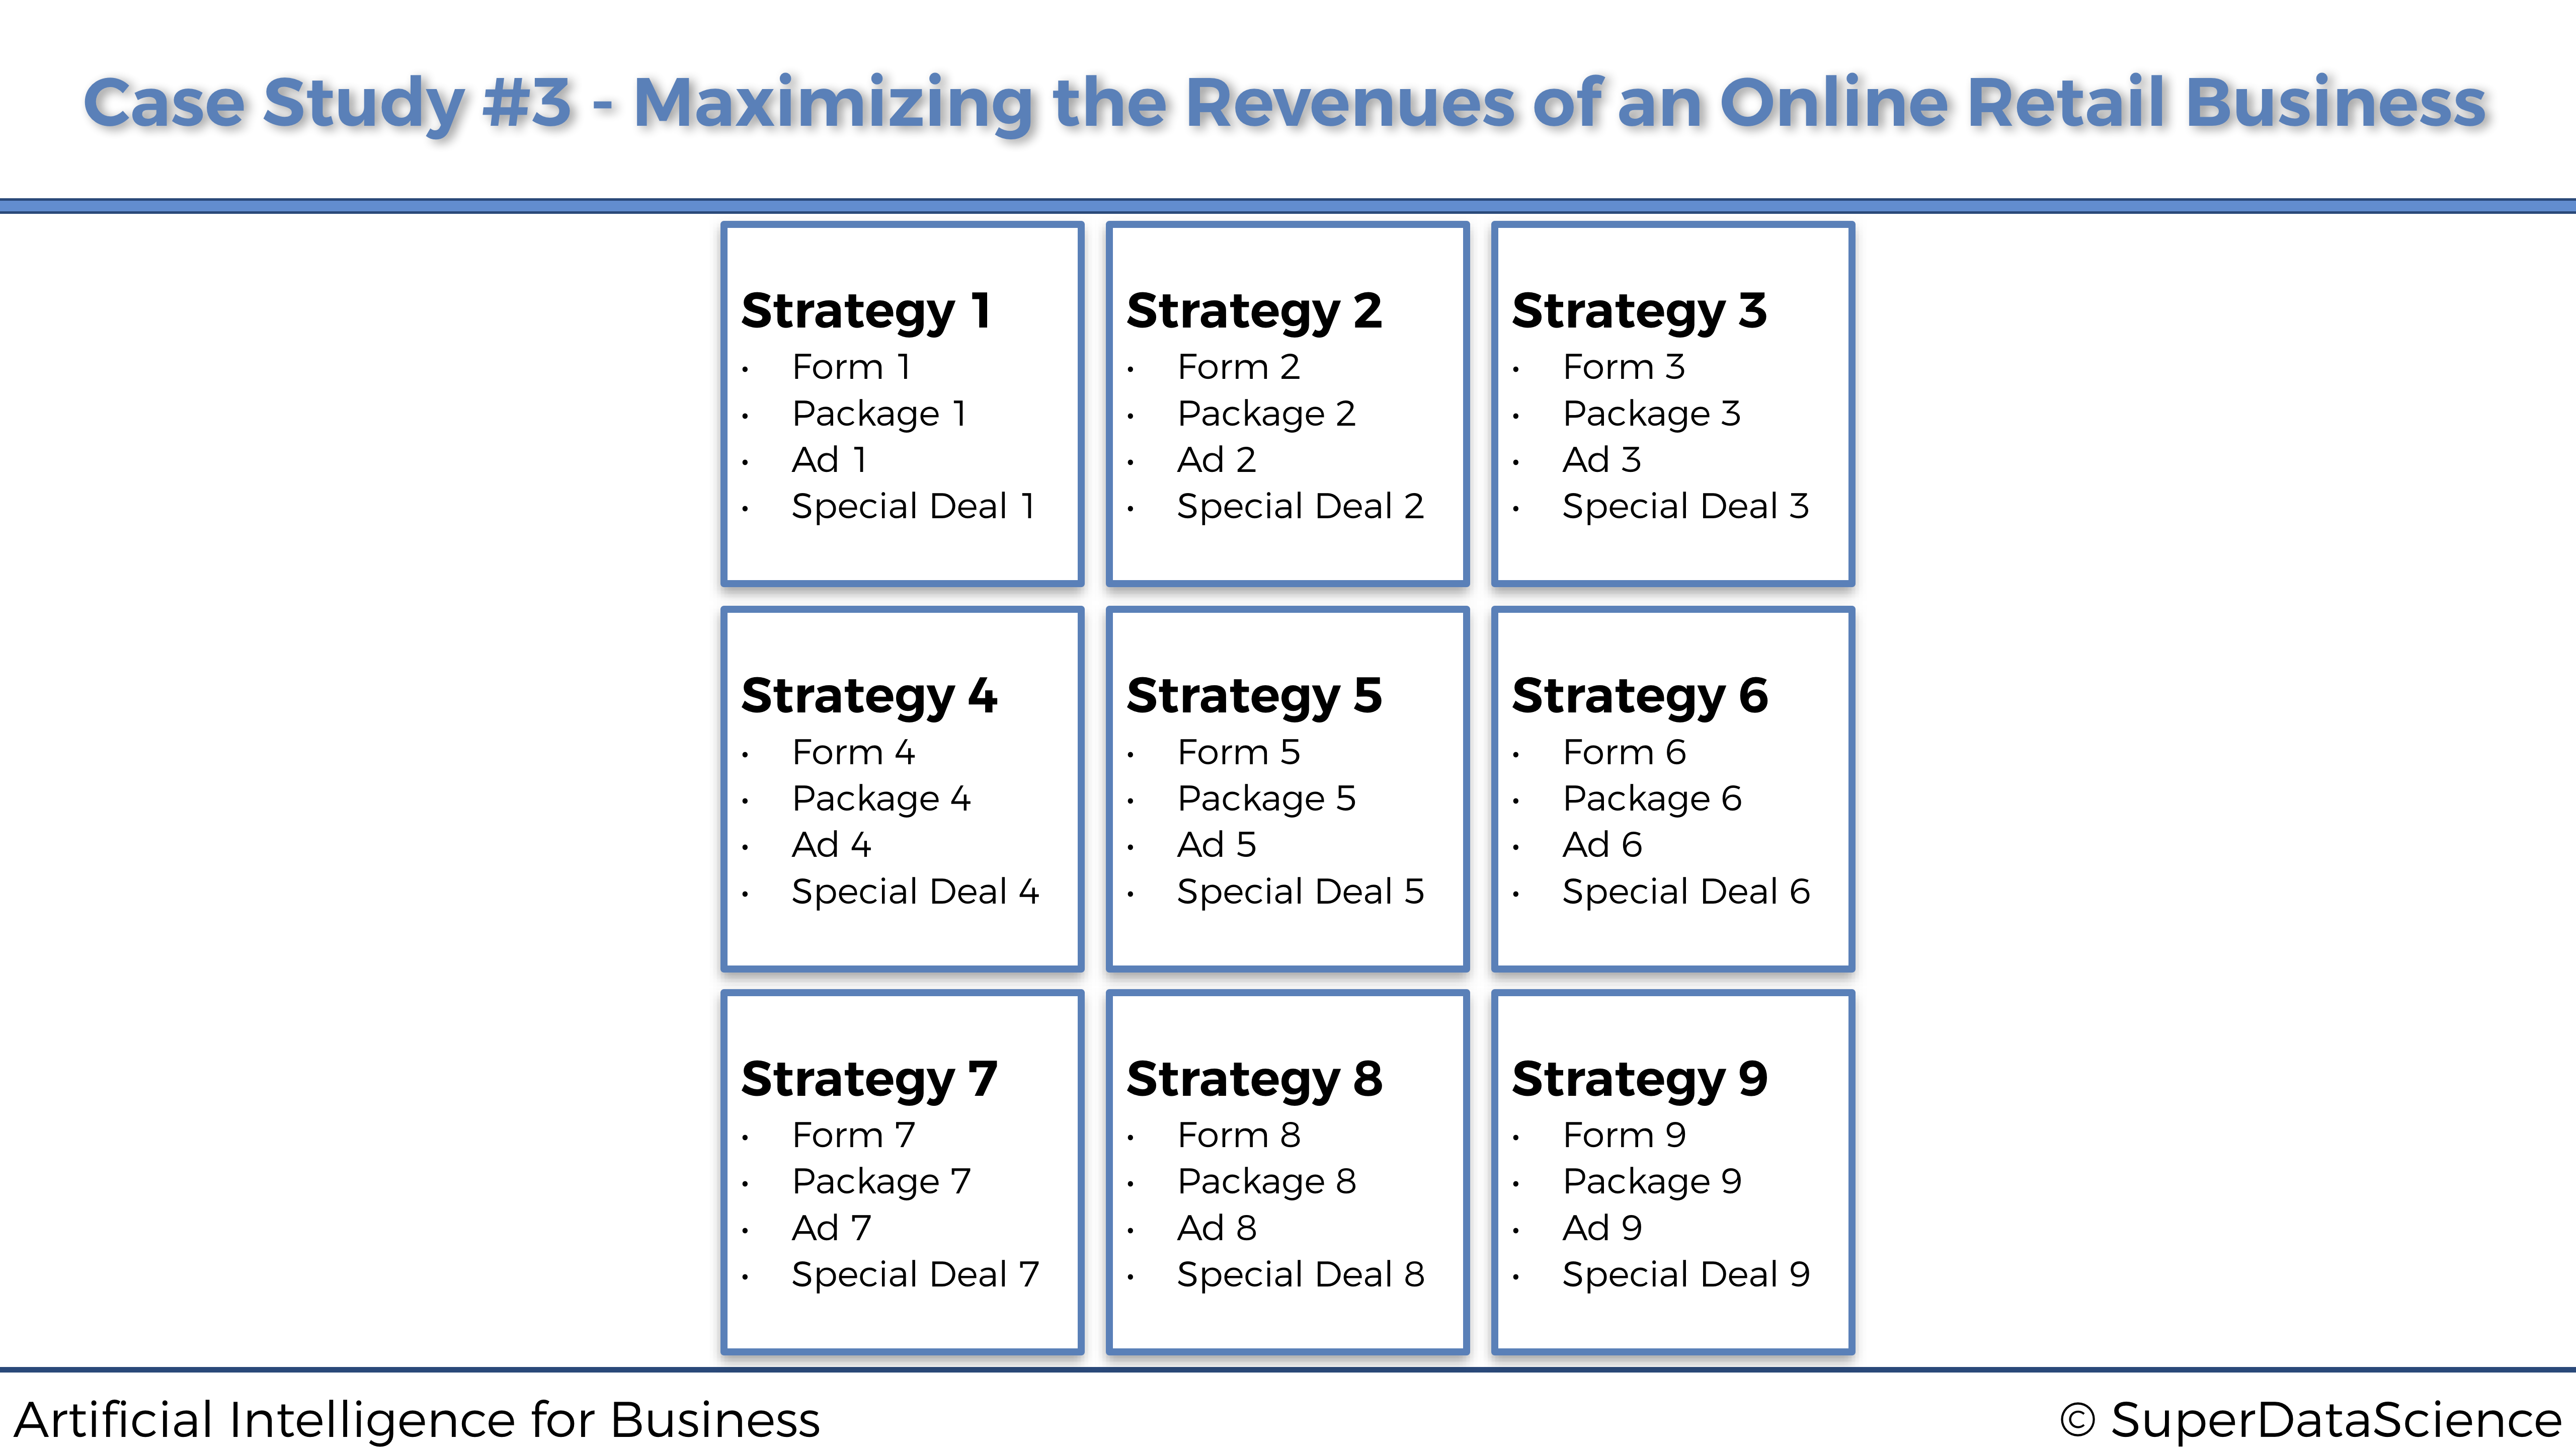
\includegraphics{Images/Strategies_Slide.png}

\textbf{Simulación}

Para simular este Caso Práctico, asumiremos que estas estrategias tienen las siguientes tasas de conversión:

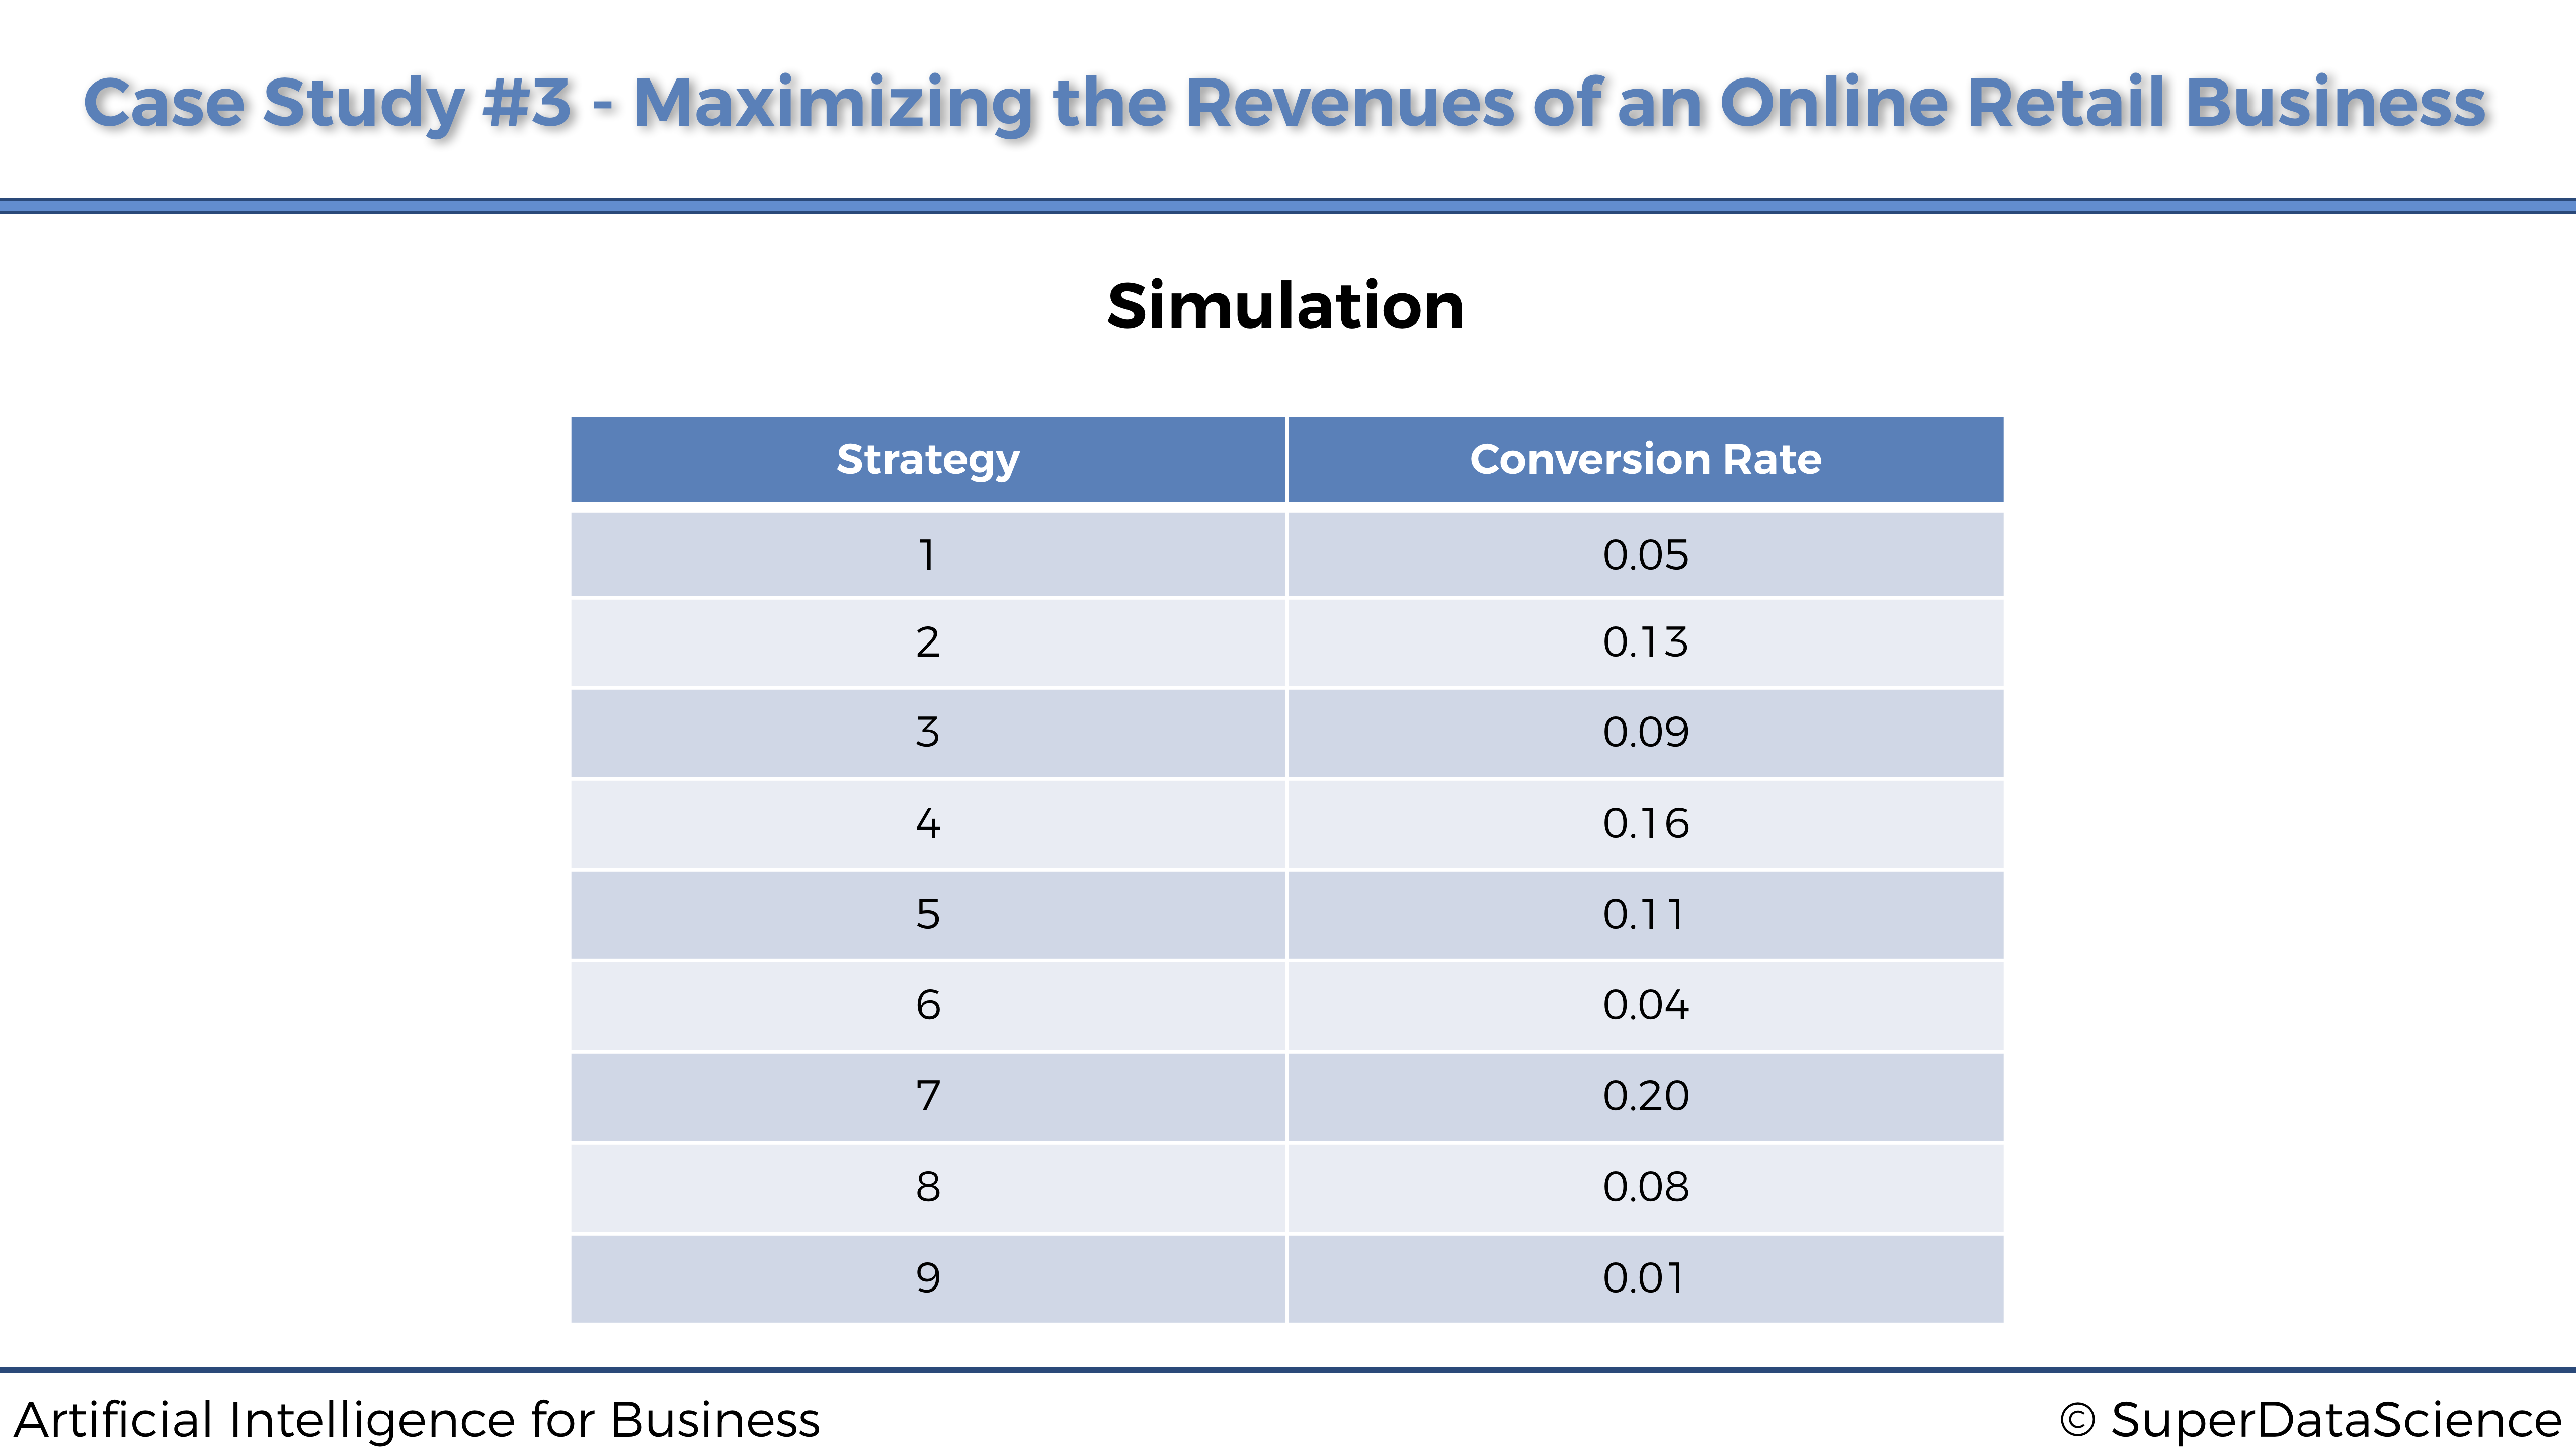
\includegraphics{Images/Simulation_Slide.png}

Sin embargo, asegúrate de comprender que en una situación de la vida real \textbf{no tendríamos idea} de cuáles serían estas tasas de conversión. Solo las conocemos aquí para fines de simulación, solo para que podamos verificar al final que nuestra IA logra descubrir la mejor estrategia, que según la tabla anterior, es la estrategia número 7 (la que tiene la tasa de conversión más alta).

\hypertarget{definiciuxf3n-del-entorno}{%
\subsection{Definición del Entorno}\label{definiciuxf3n-del-entorno}}

El aprendizaje en línea es una rama especial de la inteligencia artificial, donde no hay mucha necesidad de definir los estados y las acciones. Aquí, un estado sería simplemente un cliente específico en el que desplegaríamos una estrategia, y la acción sería simplemente la estrategia seleccionada. Luego lo verás más claro en el algoritmo de IA, donde no tenemos los estados como entradas y las acciones como salidas como en nuestros dos casos prácticos anteriores, porque esta vez no estamos haciendo Q-Learning o Deep Q-Learning. Aquí estamos haciendo aprendizaje en línea. Sin embargo, tenemos que definir las recompensas, ya que nuevamente tendremos que hacer una matriz de recompensas, donde cada fila corresponde a un usuario que está implementando una estrategia, y cada columna corresponde a una de las 9 estrategias. Por lo tanto, dado que realmente ejecutaremos este experimento de aprendizaje en línea en 10.000 clientes, esta matriz de recompensas tendrá 10.000 filas y 9 columnas. Luego, cada celda obtendrá un 0 si el cliente no se suscribe al plan premium después de ser abordado por la estrategia seleccionada, y un 1 si el cliente se suscribe después de ser abordado por la estrategia seleccionada. Y los valores en la celda son exactamente, las recompensas.

Ahora, una cosa muy importante para entender es que la matriz de recompensas solo está aquí para la simulación, y en la vida real no tendríamos una matriz de recompensas. Simplemente simularemos 10.000 clientes siendo abordados sucesivamente por una de las 9 estrategias, y gracias a la matriz de recompensas simularemos la decisión del cliente de suscribirse sí o no al plan premium. Si la celda correspondiente a un cliente específico y una estrategia seleccionada específica tiene un 1, eso simulará una conversión por parte del cliente al plan premium, y si la celda tiene un 0, simulará un rechazo. A continuación, como ejemplo, las primeras filas de una matriz de recompensas simulada:

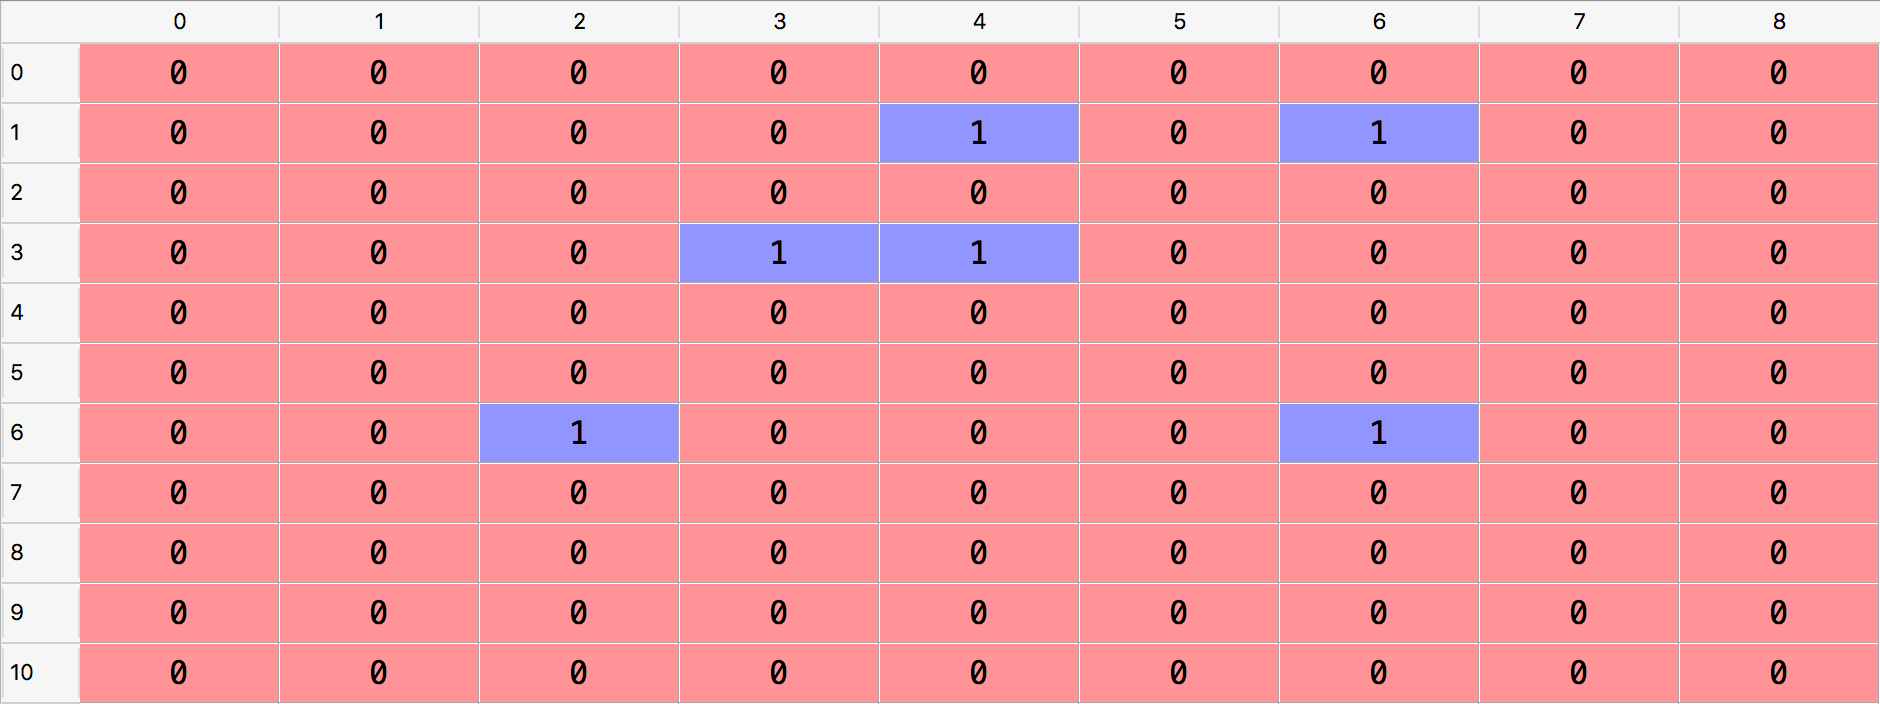
\includegraphics{Images/Rewards_Matrix.png}

De acuerdo con esta simulación, todo dado en la matriz de recompensas anterior:

\begin{enumerate}
\def\labelenumi{\arabic{enumi}.}
\tightlist
\item
  El primer cliente (fila con índice 0) no se suscribirá al plan premium después de haber sido abordado por cualquier estrategia.
\item
  El segundo cliente (fila con índice 1) se suscribiría al plan premium después de ser abordado únicamente por la estrategia 5 o la estrategia 7.
\item
  El tercer cliente (fila con índice 2) no se suscribiría al plan premium después de haber sido abordado por cualquier estrategia.
\end{enumerate}

El muestreo de Thompson recopilará los comentarios de si cada uno de estos clientes se suscribe al plan premium uno tras otro y, gracias a su poderoso algoritmo, descubrirá rápidamente la estrategia con la tasa de conversión más alta, esa es la mejor. para ser implementado en los millones de clientes, maximizando así los ingresos de la compañía de esta nueva fuente de ingresos.

\hypertarget{soluciuxf3n-de-ia-1}{%
\section{Solución de IA}\label{soluciuxf3n-de-ia-1}}

La solución de IA que determinará la mejor estrategia se llama \emph{muestreo de Thompson}. Es, con diferencia, el mejor modelo para ese tipo de problemas en esta rama de Aprendizaje en línea de Inteligencia Artificial. En resumen, cada vez que un nuevo cliente se conecta al sitio web de negocios minoristas en línea, esa es una nueva ronda \(n\) y seleccionamos una de nuestras 9 estrategias para intentar una conversión (suscripción al plan premium). El objetivo es seleccionar la mejor estrategia en cada ronda, y entrenar durante muchas rondas. Así es como el muestreo de Thompson lo hará:

\textbf{Para cada ronda \(n\), repetimos durante más de 1000 iteraciones, los siguientes tres pasos}:

\textbf{Paso 1} Para cada iteración \(i\), se elige un valor aleatorio que siga la distribución:

\[\theta_i(n) \sim \beta(N_i^1(n)+1,N_i^0(n)+1)\]

donde:

\begin{itemize}
\tightlist
\item
  \(N_i^1(n)\) es el número de veces que la estrategia \(i\)-ésima ha recibido una recompensa igual a 1 hasta la ronda \(n\)-ésima,
\item
  \(N_i^0(n)\) es el número de veces que la estrategia \(i\)-ésima ha recibido una recompensa igual a 0 hasta la ronda \(n\)-ésima.
\end{itemize}

\textbf{Paso 2} Seleccionamos la estrategia \(s(n)\) que nos da el mayor valor\(\theta_i(n)\):

\[s(n) = \underset{i\in\{1,...,9\}}{\textrm{argmax}}(\theta_i(n))\]

\textbf{Paso 3} Actualizamos \(N_{s(n)}^1(n)\) y \(N_{s(n)}^0(n)\) según las siguientes condiciones:

\begin{itemize}
\tightlist
\item
  Si la estrategia seleccionada \(s(n)\) tiene una recompensa igual a 1:
\end{itemize}

\[N_{s(n)}^1(n) := N_{s(n)}^1(n) + 1\]

\begin{itemize}
\tightlist
\item
  Si la estrategia seleccionada \(s(n)\) tiene una recompensa igual a 0:
\end{itemize}

\[N_{s(n)}^0(n) := N_{s(n)}^0(n) + 1\]

\textbf{Intuición.} Cada estrategia tiene su propia distribución beta. A lo largo de las rondas, la distribución beta de la estrategia con la tasa de conversión más alta se desplazará progresivamente hacia la derecha, y las distribuciones beta de las estrategias con tasas de conversión más bajas se desplazarán progresivamente hacia la izquierda (Pasos 1 y 3). Por lo tanto, debido al Paso 2, la estrategia con la tasa de conversión más alta se seleccionará por probabilidad cada vez más. A continuación se muestra un gráfico que muestra tres distribuciones beta de tres estrategias, que te ayudarán a visualizar este hecho:

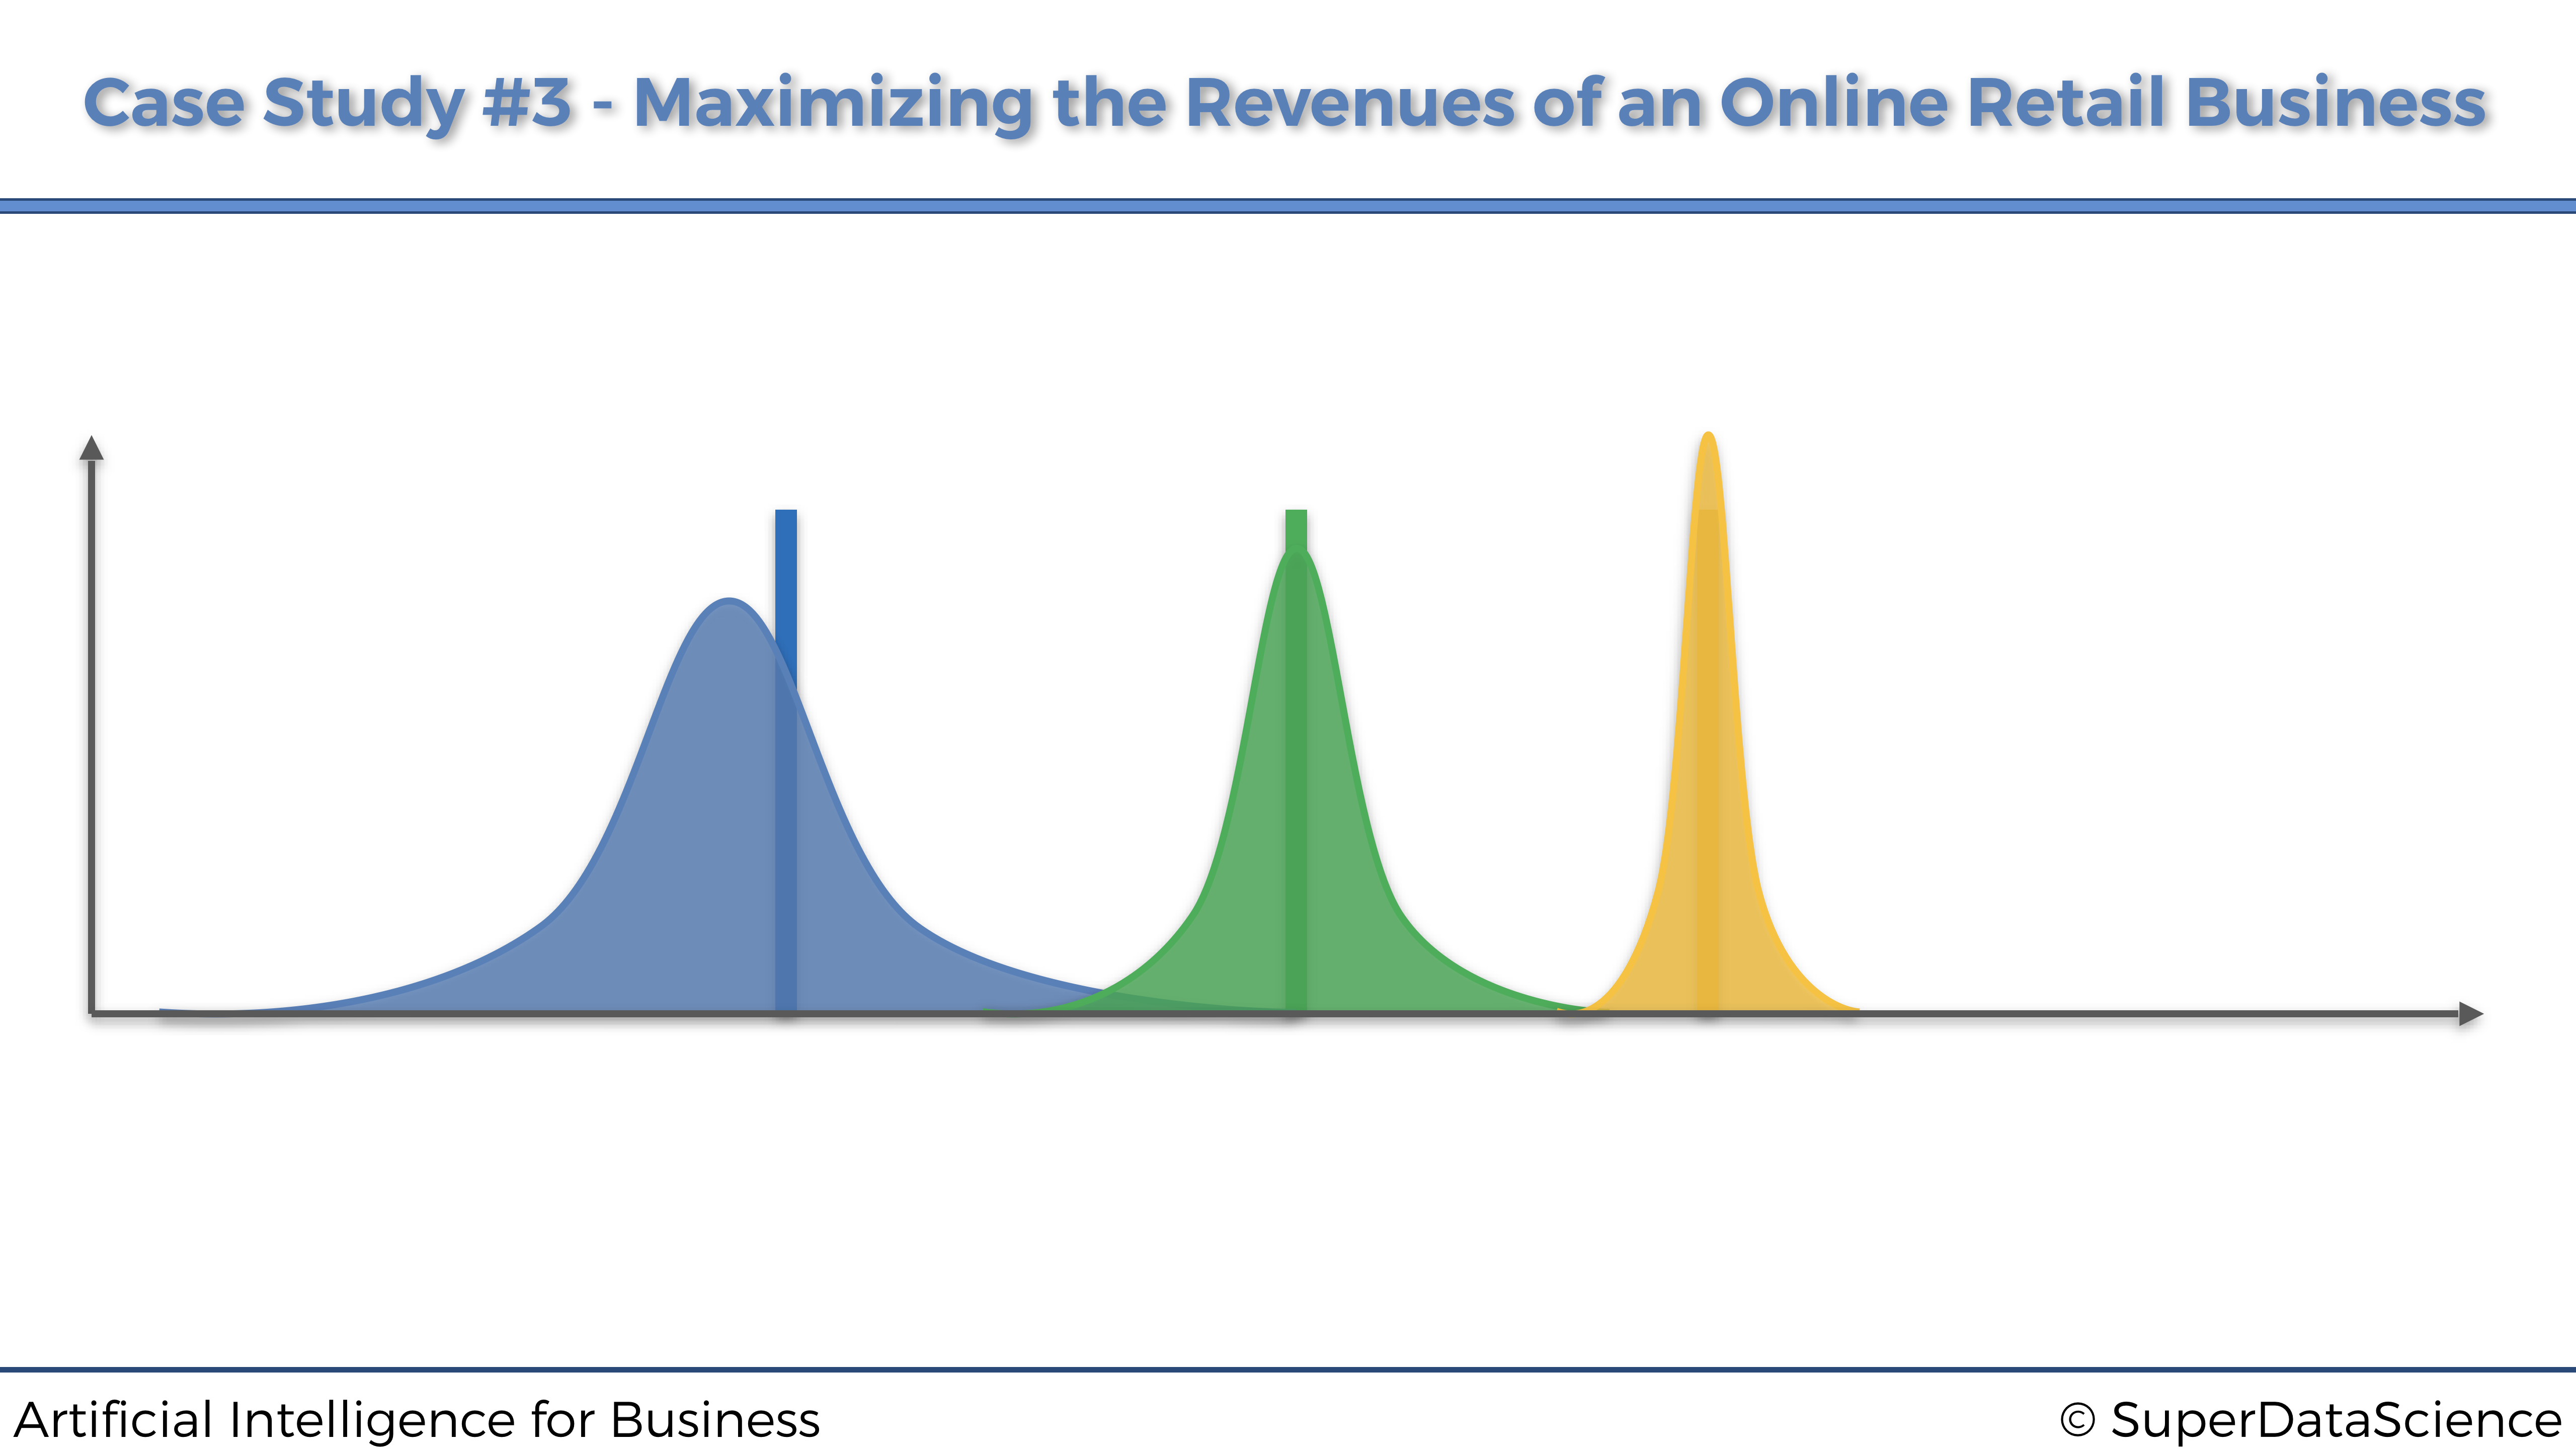
\includegraphics{Images/Beta_Distribution_Slide.png}

\hypertarget{implementaciuxf3n-1}{%
\section{Implementación}\label{implementaciuxf3n-1}}

Vamos a ver a continuación la implementación completa del muestreo de Thompson para este caso práctico específico, siguiendo la misma simulación vista anteriormente.

Al implementar el muestreo de Thompson, también implementaremos el algoritmo de selección aleatoria, que simplemente seleccionará una estrategia aleatoria en cada ronda. Este será nuestro punto de referencia para evaluar el rendimiento de nuestro modelo de muestreo de Thompson. Por supuesto, el muestreo de Thompson y el algoritmo de selección aleatoria competirán en la misma simulación, es decir, utilizando la misma matriz de recompensas. Y al final, una vez realizada la simulación completa, evaluaremos el rendimiento de Thompson Sampling calculando el rendimiento relativo, definido por la siguiente fórmula:

\[\textrm{Rendimiento Rel.} = \frac{\textrm{(Rec. del m. de Thompson)} - (\textrm{Rec. de la sel. Aleatoria})}{\textrm{Recompensa de la s. Aleatoria}} \times 100\]

También representaremos el histograma de los anuncios seleccionados, solo para verificar que la estrategia con la tasa de conversión más alta (Estrategia 7) ha sido en efecto la más seleccionada.

Pues si estás listo, aquí vamos:

Primero, importamos las librerías necesarias y establecemos los parámetros (\(N = 10000\) clientes y \(d = 9\) estrategias):

\begin{Shaded}
\begin{Highlighting}[]
\CommentTok{# Inteligencia Artificial aplicada a Negocios y Empresas}
\CommentTok{# Maximizando los ingresos de un negocio minorista en línea con el muestreo de Thompson}

\CommentTok{# Importar las librerías}
\ImportTok{import}\NormalTok{ numpy }\ImportTok{as}\NormalTok{ np}
\ImportTok{import}\NormalTok{ matplotlib.pyplot }\ImportTok{as}\NormalTok{ plt}
\ImportTok{import}\NormalTok{ random}

\CommentTok{# Configuración de parámetros}
\NormalTok{N }\OperatorTok{=} \DecValTok{10000}
\NormalTok{d }\OperatorTok{=} \DecValTok{9}
\end{Highlighting}
\end{Shaded}

Luego, creamos la simulación, construyendo la matriz de recompensas de 10000 filas correspondientes a los clientes, y 9 columnas correspondientes a las estrategias. En cada ronda y para cada estrategia, seleccionamos un número aleatorio entre 0 y 1, y si este número aleatorio es menor que la tasa de conversión de dicha estrategia, la recompensa será 1; de lo contrario, será 0. De esa manera simulamos las tasas de conversión enumeradas anteriormente para nuestras 9 estrategias:

\begin{Shaded}
\begin{Highlighting}[]
\CommentTok{# Creación de la simulación}
\NormalTok{conversion_rates }\OperatorTok{=}\NormalTok{ [}\FloatTok{0.05}\NormalTok{,}\FloatTok{0.13}\NormalTok{,}\FloatTok{0.09}\NormalTok{,}\FloatTok{0.16}\NormalTok{,}\FloatTok{0.11}\NormalTok{,}\FloatTok{0.04}\NormalTok{,}\FloatTok{0.20}\NormalTok{,}\FloatTok{0.08}\NormalTok{,}\FloatTok{0.01}\NormalTok{]}
\NormalTok{X }\OperatorTok{=}\NormalTok{ np.array(np.zeros([N,d]))}
\ControlFlowTok{for}\NormalTok{ i }\KeywordTok{in} \BuiltInTok{range}\NormalTok{(N):}
    \ControlFlowTok{for}\NormalTok{ j }\KeywordTok{in} \BuiltInTok{range}\NormalTok{(d):}
        \ControlFlowTok{if}\NormalTok{ np.random.rand() }\OperatorTok{<=}\NormalTok{ conversion_rates[j]:}
\NormalTok{            X[i,j] }\OperatorTok{=} \DecValTok{1}
\end{Highlighting}
\end{Shaded}

Luego, recorreremos las 10000 filas (o rondas) de esta matriz de recompensas, y en cada ronda obtendremos dos selecciones de estrategia separadas: una del algoritmo de Selección aleatoria y otra del muestreo de Thompson. Llevamos un registro de las estrategias seleccionadas por cada uno de estos dos algoritmos, y calculamos la recompensa total acumulada durante las rondas por cada uno de ellos. El muestreo de Thompson se implementa siguiendo exactamente los pasos 1, 2 y 3 proporcionados anteriormente:

\begin{Shaded}
\begin{Highlighting}[]
\CommentTok{# Implementación de la selección aleatoria y del muestreo de Thompson}
\NormalTok{strategies_selected_rs }\OperatorTok{=}\NormalTok{ []}
\NormalTok{strategies_selected_ts }\OperatorTok{=}\NormalTok{ []}
\NormalTok{total_reward_rs }\OperatorTok{=} \DecValTok{0}
\NormalTok{total_reward_ts }\OperatorTok{=} \DecValTok{0}
\NormalTok{numbers_of_rewards_1 }\OperatorTok{=}\NormalTok{ [}\DecValTok{0}\NormalTok{] }\OperatorTok{*}\NormalTok{ d}
\NormalTok{numbers_of_rewards_0 }\OperatorTok{=}\NormalTok{ [}\DecValTok{0}\NormalTok{] }\OperatorTok{*}\NormalTok{ d}
\ControlFlowTok{for}\NormalTok{ n }\KeywordTok{in} \BuiltInTok{range}\NormalTok{(}\DecValTok{0}\NormalTok{, N):}
    \CommentTok{# Selección aleatoria}
\NormalTok{    strategy_rs }\OperatorTok{=}\NormalTok{ random.randrange(d)}
\NormalTok{    strategies_selected_rs.append(strategy_rs)}
\NormalTok{    reward_rs }\OperatorTok{=}\NormalTok{ X[n, strategy_rs]}
\NormalTok{    total_reward_rs }\OperatorTok{=}\NormalTok{ total_reward_rs }\OperatorTok{+}\NormalTok{ reward_rs}
    \CommentTok{# Muestreo de Thompson}
\NormalTok{    strategy_ts }\OperatorTok{=} \DecValTok{0}
\NormalTok{    max_random }\OperatorTok{=} \DecValTok{0}
    \ControlFlowTok{for}\NormalTok{ i }\KeywordTok{in} \BuiltInTok{range}\NormalTok{(}\DecValTok{0}\NormalTok{, d):}
\NormalTok{        random_beta }\OperatorTok{=}\NormalTok{ random.betavariate(numbers_of_rewards_1[i] }\OperatorTok{+} \DecValTok{1}\NormalTok{,}
\NormalTok{                                         numbers_of_rewards_0[i] }\OperatorTok{+} \DecValTok{1}\NormalTok{)}
        \ControlFlowTok{if}\NormalTok{ random_beta }\OperatorTok{>}\NormalTok{ max_random:}
\NormalTok{            max_random }\OperatorTok{=}\NormalTok{ random_beta}
\NormalTok{            strategy_ts }\OperatorTok{=}\NormalTok{ i}
\NormalTok{    reward_ts }\OperatorTok{=}\NormalTok{ X[n, strategy_ts]}
    \ControlFlowTok{if}\NormalTok{ reward_ts }\OperatorTok{==} \DecValTok{1}\NormalTok{:}
\NormalTok{        numbers_of_rewards_1[strategy_ts] }\OperatorTok{=}\NormalTok{ numbers_of_rewards_1[strategy_ts] }\OperatorTok{+} \DecValTok{1}
    \ControlFlowTok{else}\NormalTok{:}
\NormalTok{        numbers_of_rewards_0[strategy_ts] }\OperatorTok{=}\NormalTok{ numbers_of_rewards_0[strategy_ts] }\OperatorTok{+} \DecValTok{1}
\NormalTok{    strategies_selected_ts.append(strategy_ts)}
\NormalTok{    total_reward_ts }\OperatorTok{=}\NormalTok{ total_reward_ts }\OperatorTok{+}\NormalTok{ reward_ts}
\end{Highlighting}
\end{Shaded}

Luego calculamos resultado final, que es el rendimiento relativo del muestreo de Thompson con respecto a nuestro punto de referencia que es la selección aleatoria:

\begin{Shaded}
\begin{Highlighting}[]
\CommentTok{# Cálculo del rendimiento relativo}
\NormalTok{relative_return }\OperatorTok{=}\NormalTok{ (total_reward_ts }\OperatorTok{-}\NormalTok{ total_reward_rs) }\OperatorTok{/}\NormalTok{ total_reward_rs }\OperatorTok{*} \DecValTok{100}
\BuiltInTok{print}\NormalTok{(}\StringTok{"Rendimiento Relativo: }\SpecialCharTok{\{:.0f\}}\StringTok{ %"}\NormalTok{.}\BuiltInTok{format}\NormalTok{(relative_return))}
\end{Highlighting}
\end{Shaded}

Y prepárate, porque al ejecutar este código obtenemos un retorno relativo final, de \ldots{}:

\begin{verbatim}
## Rendimiento Relativo: 104 %
\end{verbatim}

En otras palabras, el muestreo de Thompson casi duplicó el rendimiento de nuestro punto de referencia de la selección aleatoria.

Y finalmente, representemos el histograma de las estrategias seleccionadas, para verificar que efectivamente la Estrategia 7 (la de índice 6) fue la más seleccionada por el algoritmo, ya que es la que tiene la tasa de conversión más alta:¡

\begin{Shaded}
\begin{Highlighting}[]
\CommentTok{# Representación del histograma de selecciones}
\NormalTok{plt.hist(strategies_selected_ts)}
\end{Highlighting}
\end{Shaded}

\begin{verbatim}
## (array([   33.,   113.,   143.,   415.,     0.,    93.,    41.,  9011.,
##          118.,    33.]), array([ 0. ,  0.8,  1.6,  2.4,  3.2,  4. ,  4.8,  5.6,  6.4,  7.2,  8. ]), <a list of 10 Patch objects>)
\end{verbatim}

\begin{Shaded}
\begin{Highlighting}[]
\NormalTok{plt.title(}\StringTok{'Histograma de Selecciones'}\NormalTok{)}
\NormalTok{plt.xlabel(}\StringTok{'Estrategia'}\NormalTok{)}
\NormalTok{plt.ylabel(}\StringTok{'Numero de veces que se ha seleccionado la estrategia'}\NormalTok{)}
\NormalTok{plt.show()}
\end{Highlighting}
\end{Shaded}

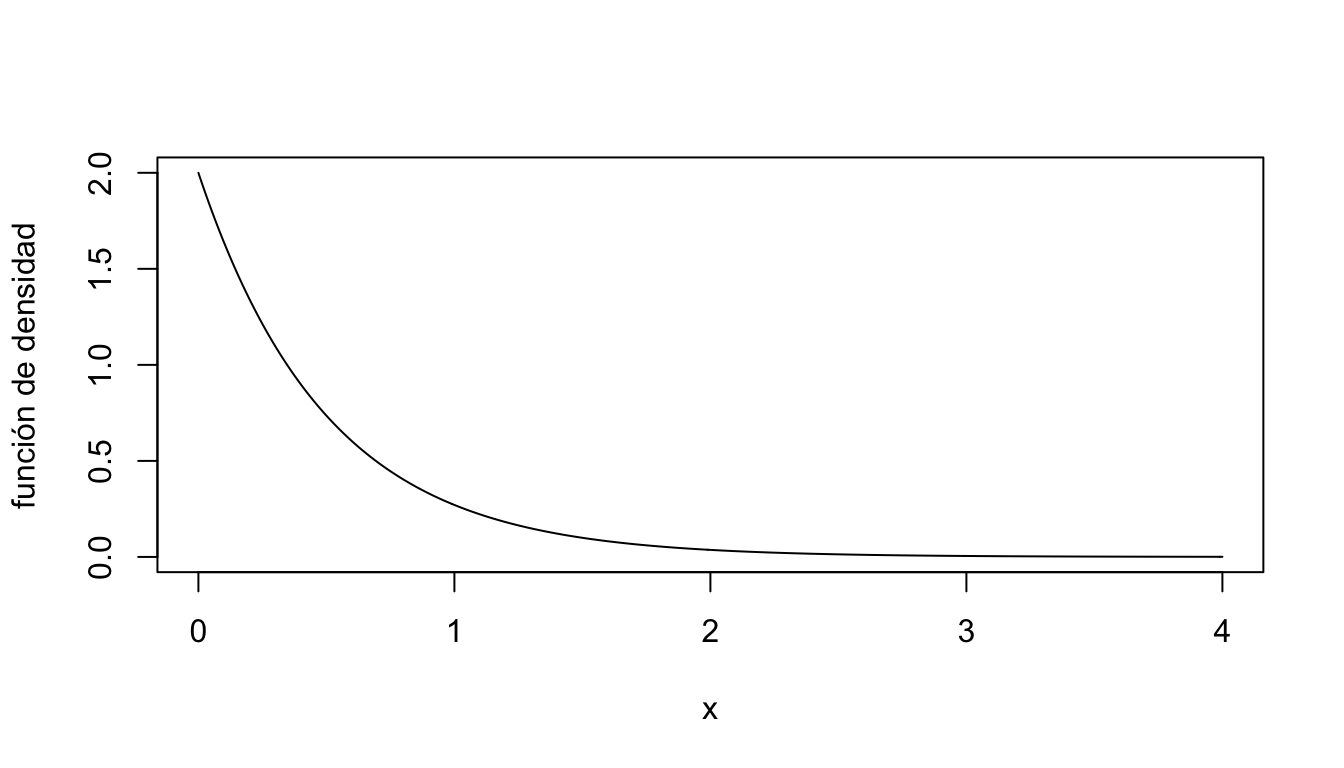
\includegraphics{/Users/juangabriel/Developer/Projects/Matematicas/bookdown-iabusiness/curso-ia-business-udemy_files/figure-latex/unnamed-chunk-37-1.pdf}

Al ejecutar este código final, obtenemos el siguiente histograma:

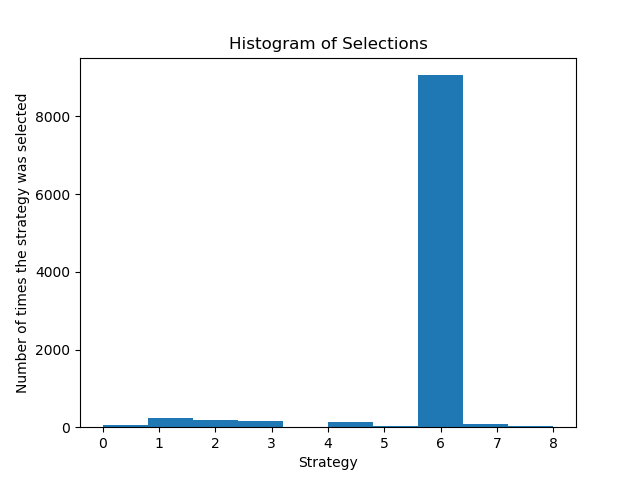
\includegraphics{Images/Histogram.png}

Y de hecho, es la estrategia del índice 6, es decir, la Estrategia 7, la que fue, con diferencia, la más seleccionada. El muestreo de Thompson ha sido capaz de identificarlo rápidamente. Y, de hecho, si volvemos a ejecutar el mismo código pero con solo 1000 clientes, nos damos cuenta de que el muestreo de Thompson todavía puede identificar la Estrategia 7 como la mejor, con muchas menos pruebas.

En consecuencia, el muestreo de Thompson seguramente ha hecho un trabajo increíble para este negocio minorista en línea. Porque no solo ha sido capaz de identificar la mejor estrategia rápidamente en un número reducido de rondas, es decir, con solamente algunos clientes, lo que nos ha ahorrado mucho en publicidad y costes operativos. Pero también, por supuesto, ha sido capaz de descubrir claramente la estrategia con la tasa de conversión más alta. Y, de hecho, si este negocio minorista en línea tiene 100 millones de clientes, y si el plan premium tiene un precio de 100 dólares al año, la implementación de esta mejor estrategia que tiene una tasa de conversión del 20\% conduciría a generar un ingreso adicional de \ldots{}:

\[\textrm{Ingresos extra generados} = 100000000 \times 0.2 \times 100 = \textrm{2 mil millones de }\$!!\]

En otras palabras, muestreo de Thompson maximizó clara y rápidamente los ingresos de este negocio minorista en línea, al mismo tiempo que ahorró mucho en los costos, maximizando así la rentabilidad del negocio.

\textbf{Curva del arrepentimiento.}

La curva de arrepentimiento de un modelo (con estrategia aleatoria o con el muestreo de Sampling) es la representación gráfica de la diferencia entre la mejor estrategia y el modelo desplegado, con respecto a las rondas.

La mejor estrategia se calcula simplemente obteniendo, en cada ronda, el máximo de las recompensas acumuladas sobre todas las diferentes estrategias. Por lo tanto, en nuestra implementación, obtendremos la mejor estrategia de la siguiente manera:

\begin{Shaded}
\begin{Highlighting}[]
\NormalTok{rewards_strategies }\OperatorTok{=}\NormalTok{ [}\DecValTok{0}\NormalTok{] }\OperatorTok{*}\NormalTok{ d}
\ControlFlowTok{for}\NormalTok{ n }\KeywordTok{in} \BuiltInTok{range}\NormalTok{(}\DecValTok{0}\NormalTok{, N):}
    \CommentTok{# La mejor estrategia}
    \ControlFlowTok{for}\NormalTok{ i }\KeywordTok{in} \BuiltInTok{range}\NormalTok{(}\DecValTok{0}\NormalTok{, d):}
\NormalTok{        rewards_strategies[i] }\OperatorTok{=}\NormalTok{ rewards_strategies[i] }\OperatorTok{+}\NormalTok{ X[n, i]}
\NormalTok{    total_reward_bs }\OperatorTok{=} \BuiltInTok{max}\NormalTok{(rewards_strategies)}
\end{Highlighting}
\end{Shaded}

Entonces, el arrepentimiento del muestreo de Thompson se calcula simplemente como la diferencia entre la mejor estrategia y el modelo del muestreo de Thompson:

\begin{Shaded}
\begin{Highlighting}[]
\CommentTok{# Arrepentimiento del muestreo Thompson}
\NormalTok{strategies_selected_ts }\OperatorTok{=}\NormalTok{ []}
\NormalTok{total_reward_ts }\OperatorTok{=} \DecValTok{0}
\NormalTok{total_reward_bs }\OperatorTok{=} \DecValTok{0}
\NormalTok{numbers_of_rewards_1 }\OperatorTok{=}\NormalTok{ [}\DecValTok{0}\NormalTok{] }\OperatorTok{*}\NormalTok{ d}
\NormalTok{numbers_of_rewards_0 }\OperatorTok{=}\NormalTok{ [}\DecValTok{0}\NormalTok{] }\OperatorTok{*}\NormalTok{ d}
\NormalTok{rewards_strategies }\OperatorTok{=}\NormalTok{ [}\DecValTok{0}\NormalTok{] }\OperatorTok{*}\NormalTok{ d}
\NormalTok{regret }\OperatorTok{=}\NormalTok{ []}
\ControlFlowTok{for}\NormalTok{ n }\KeywordTok{in} \BuiltInTok{range}\NormalTok{(}\DecValTok{0}\NormalTok{, N):}
    \CommentTok{# Muestreo de Thompson}
\NormalTok{    strategy_ts }\OperatorTok{=} \DecValTok{0}
\NormalTok{    max_random }\OperatorTok{=} \DecValTok{0}
    \ControlFlowTok{for}\NormalTok{ i }\KeywordTok{in} \BuiltInTok{range}\NormalTok{(}\DecValTok{0}\NormalTok{, d):}
\NormalTok{        random_beta }\OperatorTok{=}\NormalTok{ random.betavariate(numbers_of_rewards_1[i] }\OperatorTok{+} \DecValTok{1}\NormalTok{,}
\NormalTok{                                         numbers_of_rewards_0[i] }\OperatorTok{+} \DecValTok{1}\NormalTok{)}
        \ControlFlowTok{if}\NormalTok{ random_beta }\OperatorTok{>}\NormalTok{ max_random:}
\NormalTok{            max_random }\OperatorTok{=}\NormalTok{ random_beta}
\NormalTok{            strategy_ts }\OperatorTok{=}\NormalTok{ i}
\NormalTok{    reward_ts }\OperatorTok{=}\NormalTok{ X[n, strategy_ts]}
    \ControlFlowTok{if}\NormalTok{ reward_ts }\OperatorTok{==} \DecValTok{1}\NormalTok{:}
\NormalTok{        numbers_of_rewards_1[strategy_ts] }\OperatorTok{=}\NormalTok{ numbers_of_rewards_1[strategy_ts] }\OperatorTok{+} \DecValTok{1}
    \ControlFlowTok{else}\NormalTok{:}
\NormalTok{        numbers_of_rewards_0[strategy_ts] }\OperatorTok{=}\NormalTok{ numbers_of_rewards_0[strategy_ts] }\OperatorTok{+} \DecValTok{1}
\NormalTok{    strategies_selected_ts.append(strategy_ts)}
\NormalTok{    total_reward_ts }\OperatorTok{=}\NormalTok{ total_reward_ts }\OperatorTok{+}\NormalTok{ reward_ts}
    \CommentTok{# La mejor estrategia}
    \ControlFlowTok{for}\NormalTok{ i }\KeywordTok{in} \BuiltInTok{range}\NormalTok{(}\DecValTok{0}\NormalTok{, d):}
\NormalTok{        rewards_strategies[i] }\OperatorTok{=}\NormalTok{ rewards_strategies[i] }\OperatorTok{+}\NormalTok{ X[n, i]}
\NormalTok{    total_reward_bs }\OperatorTok{=} \BuiltInTok{max}\NormalTok{(rewards_strategies)}
    \CommentTok{# Arrepentimiento}
\NormalTok{    regret.append(total_reward_bs }\OperatorTok{-}\NormalTok{ total_reward_ts)}
\end{Highlighting}
\end{Shaded}

Y lo mismo, el arrepentimiento de la estrategia aleatoria simplemente se calcula como la diferencia entre la mejor estrategia y el algoritmo de selección aleatoria:

\begin{Shaded}
\begin{Highlighting}[]
\CommentTok{# Arrepentimiento de la estrategia aleatoria}
\NormalTok{strategies_selected_rs }\OperatorTok{=}\NormalTok{ []}
\NormalTok{total_reward_rs }\OperatorTok{=} \DecValTok{0}
\NormalTok{total_reward_bs }\OperatorTok{=} \DecValTok{0}
\NormalTok{numbers_of_rewards_1 }\OperatorTok{=}\NormalTok{ [}\DecValTok{0}\NormalTok{] }\OperatorTok{*}\NormalTok{ d}
\NormalTok{numbers_of_rewards_0 }\OperatorTok{=}\NormalTok{ [}\DecValTok{0}\NormalTok{] }\OperatorTok{*}\NormalTok{ d}
\NormalTok{rewards_strategies }\OperatorTok{=}\NormalTok{ [}\DecValTok{0}\NormalTok{] }\OperatorTok{*}\NormalTok{ d}
\NormalTok{regret }\OperatorTok{=}\NormalTok{ []}
\ControlFlowTok{for}\NormalTok{ n }\KeywordTok{in} \BuiltInTok{range}\NormalTok{(}\DecValTok{0}\NormalTok{, N):}
    \CommentTok{# Estrategia aleatoria}
\NormalTok{    strategy_rs }\OperatorTok{=}\NormalTok{ random.randrange(d)}
\NormalTok{    strategies_selected_rs.append(strategy_rs)}
\NormalTok{    reward_rs }\OperatorTok{=}\NormalTok{ X[n, strategy_rs]}
\NormalTok{    total_reward_rs }\OperatorTok{=}\NormalTok{ total_reward_rs }\OperatorTok{+}\NormalTok{ reward_rs}
    \CommentTok{# La mejor estrategia}
    \ControlFlowTok{for}\NormalTok{ i }\KeywordTok{in} \BuiltInTok{range}\NormalTok{(}\DecValTok{0}\NormalTok{, d):}
\NormalTok{        rewards_strategies[i] }\OperatorTok{=}\NormalTok{ rewards_strategies[i] }\OperatorTok{+}\NormalTok{ X[n, i]}
\NormalTok{    total_reward_bs }\OperatorTok{=} \BuiltInTok{max}\NormalTok{(rewards_strategies)}
    \CommentTok{# Arrepentimiento}
\NormalTok{    regret.append(total_reward_bs }\OperatorTok{-}\NormalTok{ total_reward_rs)}
\end{Highlighting}
\end{Shaded}

Y finalmente, por supuesto, representamos el arrepentimiento sobre las rondas con este simple código (no tenemos que especificar las coordenadas x en la función \texttt{plt.plot()} porque las rondas ya son índices desde 0 hasta N):

\begin{Shaded}
\begin{Highlighting}[]
\CommentTok{# Representación de la curva de arrepentimiento}
\NormalTok{plt.plot(regret)}
\NormalTok{plt.title(}\StringTok{'Curva de Arrepentimiento'}\NormalTok{)}
\NormalTok{plt.xlabel(}\StringTok{'Ronda'}\NormalTok{)}
\NormalTok{plt.ylabel(}\StringTok{'Arrepentimiento'}\NormalTok{)}
\NormalTok{plt.show()}
\end{Highlighting}
\end{Shaded}

Si representamos la curva de arrepentimiento de la estrategia aleatoria, obtenemos lo siguiente:

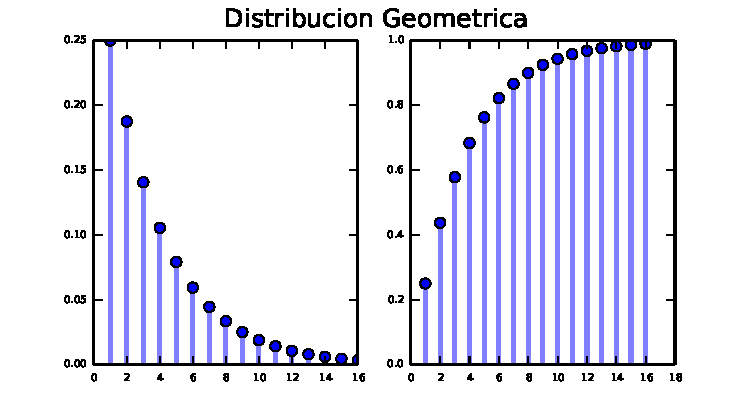
\includegraphics{/Users/juangabriel/Developer/Projects/Matematicas/bookdown-iabusiness/curso-ia-business-udemy_files/figure-latex/unnamed-chunk-43-1.pdf}

Y, por supuesto, no observamos absolutamente ninguna convergencia de la estrategia aleatoria hacia la mejor estrategia.

Sin embargo, si ahora representamos la curva de arrepentimiento del modelo de muestreo de Thompson, obtenemos la siguiente curva hermosa:

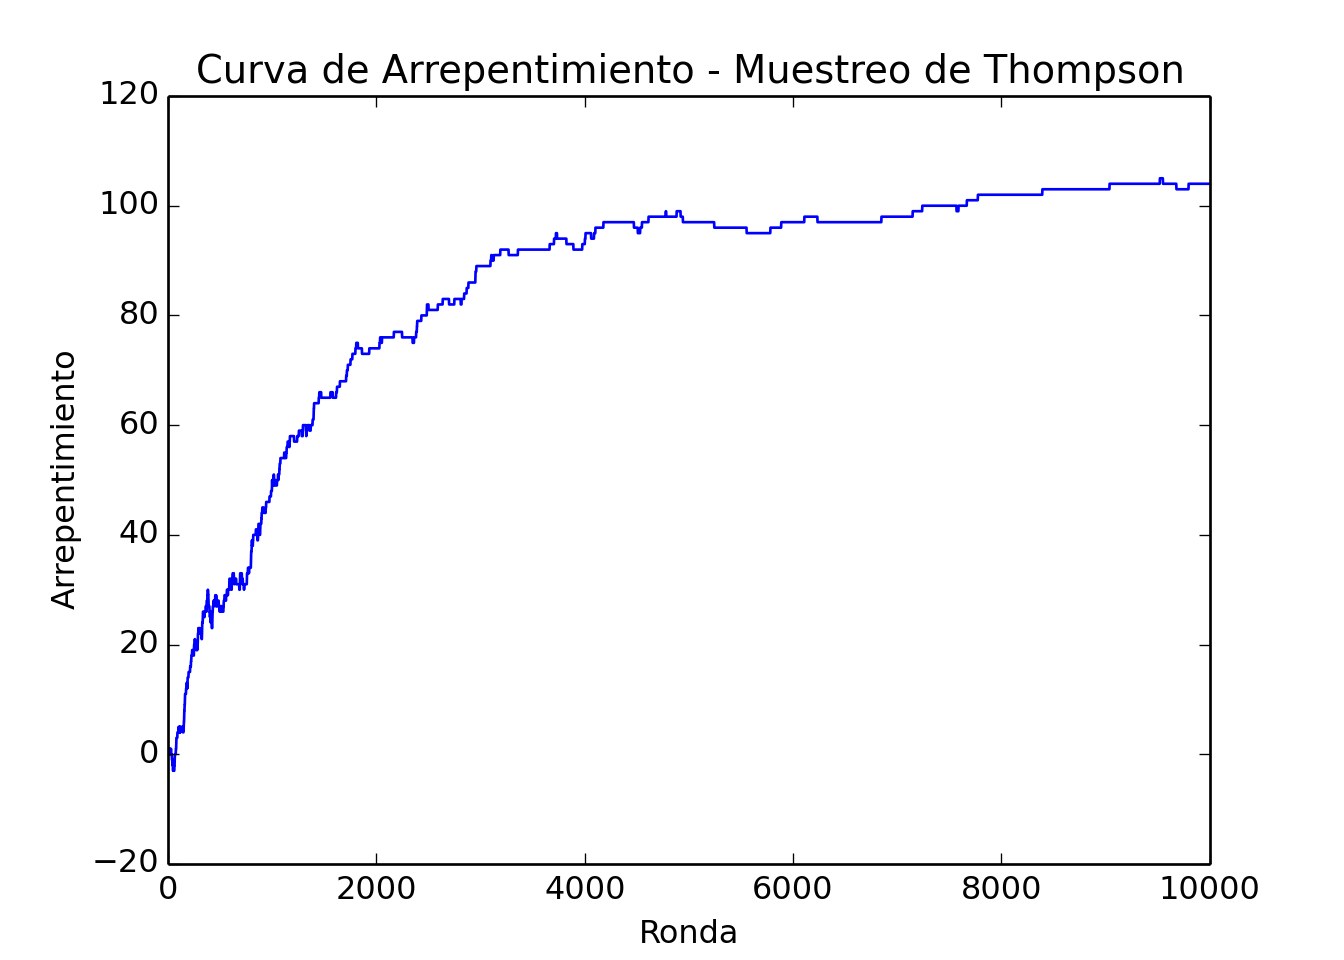
\includegraphics{/Users/juangabriel/Developer/Projects/Matematicas/bookdown-iabusiness/curso-ia-business-udemy_files/figure-latex/unnamed-chunk-44-1.pdf}
Y obviamente, el muestreo de Thompson está convergiendo muy bien hacia la mejor estrategia.

Finalmente, aquí está el código final que incluye esa Curva de arrepentimiento del muestreo de Thompson:

\begin{Shaded}
\begin{Highlighting}[]
\CommentTok{# Muestreo de Thompson}

\CommentTok{# Importar las librerías}
\ImportTok{import}\NormalTok{ numpy }\ImportTok{as}\NormalTok{ np}
\ImportTok{import}\NormalTok{ matplotlib.pyplot }\ImportTok{as}\NormalTok{ plt}
\ImportTok{import}\NormalTok{ random}

\CommentTok{# Configuración de los parámetros}
\NormalTok{N }\OperatorTok{=} \DecValTok{10000}
\NormalTok{d }\OperatorTok{=} \DecValTok{9}

\CommentTok{# Creación de la simulación}
\NormalTok{conversion_rates }\OperatorTok{=}\NormalTok{ [}\FloatTok{0.05}\NormalTok{,}\FloatTok{0.13}\NormalTok{,}\FloatTok{0.09}\NormalTok{,}\FloatTok{0.16}\NormalTok{,}\FloatTok{0.11}\NormalTok{,}\FloatTok{0.04}\NormalTok{,}\FloatTok{0.20}\NormalTok{,}\FloatTok{0.08}\NormalTok{,}\FloatTok{0.01}\NormalTok{]}
\NormalTok{X }\OperatorTok{=}\NormalTok{ np.array(np.zeros([N,d]))}
\ControlFlowTok{for}\NormalTok{ i }\KeywordTok{in} \BuiltInTok{range}\NormalTok{(N):}
    \ControlFlowTok{for}\NormalTok{ j }\KeywordTok{in} \BuiltInTok{range}\NormalTok{(d):}
        \ControlFlowTok{if}\NormalTok{ np.random.rand() }\OperatorTok{<=}\NormalTok{ conversion_rates[j]:}
\NormalTok{            X[i,j] }\OperatorTok{=} \DecValTok{1}

\CommentTok{# Implementación de la estrategia aleatoria y del muestreo de Thompson con la curva de arrepentimiento}
\NormalTok{strategies_selected_rs }\OperatorTok{=}\NormalTok{ []}
\NormalTok{strategies_selected_ts }\OperatorTok{=}\NormalTok{ []}
\NormalTok{total_reward_rs }\OperatorTok{=} \DecValTok{0}
\NormalTok{total_reward_ts }\OperatorTok{=} \DecValTok{0}
\NormalTok{total_reward_bs }\OperatorTok{=} \DecValTok{0}
\NormalTok{numbers_of_rewards_1 }\OperatorTok{=}\NormalTok{ [}\DecValTok{0}\NormalTok{] }\OperatorTok{*}\NormalTok{ d}
\NormalTok{numbers_of_rewards_0 }\OperatorTok{=}\NormalTok{ [}\DecValTok{0}\NormalTok{] }\OperatorTok{*}\NormalTok{ d}
\NormalTok{rewards_strategies }\OperatorTok{=}\NormalTok{ [}\DecValTok{0}\NormalTok{] }\OperatorTok{*}\NormalTok{ d}
\NormalTok{regret }\OperatorTok{=}\NormalTok{ []}
\ControlFlowTok{for}\NormalTok{ n }\KeywordTok{in} \BuiltInTok{range}\NormalTok{(}\DecValTok{0}\NormalTok{, N):}
    \CommentTok{# Estrategia aleatoria}
\NormalTok{    strategy_rs }\OperatorTok{=}\NormalTok{ random.randrange(d)}
\NormalTok{    strategies_selected_rs.append(strategy_rs)}
\NormalTok{    reward_rs }\OperatorTok{=}\NormalTok{ X[n, strategy_rs]}
\NormalTok{    total_reward_rs }\OperatorTok{=}\NormalTok{ total_reward_rs }\OperatorTok{+}\NormalTok{ reward_rs}
    \CommentTok{# Muestreo de Thompson}
\NormalTok{    strategy_ts }\OperatorTok{=} \DecValTok{0}
\NormalTok{    max_random }\OperatorTok{=} \DecValTok{0}
    \ControlFlowTok{for}\NormalTok{ i }\KeywordTok{in} \BuiltInTok{range}\NormalTok{(}\DecValTok{0}\NormalTok{, d):}
\NormalTok{        random_beta }\OperatorTok{=}\NormalTok{ random.betavariate(numbers_of_rewards_1[i] }\OperatorTok{+} \DecValTok{1}\NormalTok{,}
\NormalTok{                                         numbers_of_rewards_0[i] }\OperatorTok{+} \DecValTok{1}\NormalTok{)}
        \ControlFlowTok{if}\NormalTok{ random_beta }\OperatorTok{>}\NormalTok{ max_random:}
\NormalTok{            max_random }\OperatorTok{=}\NormalTok{ random_beta}
\NormalTok{            strategy_ts }\OperatorTok{=}\NormalTok{ i}
\NormalTok{    reward_ts }\OperatorTok{=}\NormalTok{ X[n, strategy_ts]}
    \ControlFlowTok{if}\NormalTok{ reward_ts }\OperatorTok{==} \DecValTok{1}\NormalTok{:}
\NormalTok{        numbers_of_rewards_1[strategy_ts] }\OperatorTok{=}\NormalTok{ numbers_of_rewards_1[strategy_ts] }\OperatorTok{+} \DecValTok{1}
    \ControlFlowTok{else}\NormalTok{:}
\NormalTok{        numbers_of_rewards_0[strategy_ts] }\OperatorTok{=}\NormalTok{ numbers_of_rewards_0[strategy_ts] }\OperatorTok{+} \DecValTok{1}
\NormalTok{    strategies_selected_ts.append(strategy_ts)}
\NormalTok{    total_reward_ts }\OperatorTok{=}\NormalTok{ total_reward_ts }\OperatorTok{+}\NormalTok{ reward_ts}
    \CommentTok{# La mejor estrategia}
    \ControlFlowTok{for}\NormalTok{ i }\KeywordTok{in} \BuiltInTok{range}\NormalTok{(}\DecValTok{0}\NormalTok{, d):}
\NormalTok{        rewards_strategies[i] }\OperatorTok{=}\NormalTok{ rewards_strategies[i] }\OperatorTok{+}\NormalTok{ X[n, i]}
\NormalTok{    total_reward_bs }\OperatorTok{=} \BuiltInTok{max}\NormalTok{(rewards_strategies)}
    \CommentTok{# Arrepentimiento}
\NormalTok{    regret.append(total_reward_bs }\OperatorTok{-}\NormalTok{ total_reward_ts)}

\CommentTok{# Calcular el rendimiento absoluto y relativo}
\NormalTok{absolute_return }\OperatorTok{=}\NormalTok{ total_reward_ts }\OperatorTok{-}\NormalTok{ total_reward_rs}
\NormalTok{relative_return }\OperatorTok{=}\NormalTok{ (total_reward_ts }\OperatorTok{-}\NormalTok{ total_reward_rs) }\OperatorTok{/}\NormalTok{ total_reward_rs }\OperatorTok{*} \DecValTok{100}
\BuiltInTok{print}\NormalTok{(}\StringTok{"Rendimiento Absoluto: }\SpecialCharTok{\{:.0f\}}\StringTok{ $"}\NormalTok{.}\BuiltInTok{format}\NormalTok{(absolute_return))}
\BuiltInTok{print}\NormalTok{(}\StringTok{"Rendimiento Relativo: }\SpecialCharTok{\{:.0f\}}\StringTok{ %"}\NormalTok{.}\BuiltInTok{format}\NormalTok{(relative_return))}

\CommentTok{# Representación de los histogramas de selecciones}
\NormalTok{plt.hist(strategies_selected_ts)}
\NormalTok{plt.title(}\StringTok{'Histograma de Selecciones'}\NormalTok{)}
\NormalTok{plt.xlabel(}\StringTok{'Estrategia'}\NormalTok{)}
\NormalTok{plt.ylabel(}\StringTok{'Numero de veces que la estrategia ha sido seleccionada'}\NormalTok{)}
\NormalTok{plt.show()}
\NormalTok{plt.close()}

\CommentTok{# Representación de la curva de arrepentimiento}
\NormalTok{plt.plot(regret)}
\NormalTok{plt.title(}\StringTok{'Curva de Arrepentimiento'}\NormalTok{)}
\NormalTok{plt.xlabel(}\StringTok{'Ronda'}\NormalTok{)}
\NormalTok{plt.ylabel(}\StringTok{'Arrepentimiento'}\NormalTok{)}
\NormalTok{plt.show()}
\end{Highlighting}
\end{Shaded}

\hypertarget{conclusiuxf3n}{%
\chapter*{Conclusión}\label{conclusiuxf3n}}
\addcontentsline{toc}{chapter}{Conclusión}

¡Muchas gracias de nuevo por unirte a este curso en Udemy y felicidades por completarlo! Te recomendamos encarecidamente que mantengas este libro cerca de ti cada vez que construyas una IA para resolver un problema comercial. O al menos, trata de mantener el algoritmo general de IA que hemos construido en cada parte del curso. Para nosotros, ha sido todo un placer hacer este curso y escribir este libro. No dudes en dejar un comentario en el curso si lo deseas. Hasta entonces, ¡disfruta de IA aplicada a Negocios y Empresas!

\hypertarget{anexos-adicionales}{%
\chapter{Anexos adicionales}\label{anexos-adicionales}}

\hypertarget{anexo-1-redes-neuronales-artificiales}{%
\section{Anexo 1: Redes Neuronales Artificiales}\label{anexo-1-redes-neuronales-artificiales}}

En este apartado Anexo, encontrarás toda la teoría necesaria de Redes Neuronales Artificiales, que son el apartado principal del modelo de Deep Q-Learning model que hemos creado en la Parte 2 - Minimización de Costes. Este es el plan de ataque que seguiremos para estudiar acerca de las Redes Neuronales Artificiales:

\begin{itemize}
\tightlist
\item
  La Neurona
\item
  La Función de Activación
\item
  ¿Cómo funcionan las Redes Neuronales?
\item
  ¿Cómo aprenden las Redes Neuronales?
\item
  Propagación hacia adelante and Propagación hacia atrás
\item
  Gradiente Descendente
\item
  Gradiente Descendente por bloques y Gradiente Descendente Estocástico
\end{itemize}

\hypertarget{la-neurona}{%
\subsection{La Neurona}\label{la-neurona}}

La neurona es el bloque de construcción básico de las redes neuronales artificiales. En las siguientes imágenes se muestran neuronas reales de la vida real que se han colocado sobre un vidrio, coloreadas un poco con tinte y observadas con un microscopio:

\includegraphics{Images/ANN_1.png}

Como podemos ver, tienen la estructura de un cuerpo con muchas ramas diferentes que salen de ellos. Pero la pregunta es: ¿cómo podemos recrear esta estructura en una máquina? De hecho, realmente necesitamos recrearlo en un ordenador, ya que el objetivo de Deep Learning es imitar cómo funciona el cerebro humano, con la esperanza de que al hacerlo creemos algo increíble: una infraestructura poderosa para que las máquinas puedan aprender.

¿Por qué esperamos eso? Porque el cerebro humano resulta ser una de las herramientas de aprendizaje más poderosas del planeta. Así que solo esperamos que si lo recreamos, tendremos algo tan increíble como eso. Entonces, este será nuestro desafío en este momento, este es nuestro primer paso para crear Redes Neuronales Artificiales: ser capaces de recrear una neurona.

Entonces, ¿cómo lo hacemos? Bueno, antes que nada echemos un vistazo más de cerca a lo que realmente es una neurona. La imagen a continuación fue creada por primera vez por un neurocientífico español Santiago Ramón y Cajal en 1899:

\includegraphics{Images/ANN_2.png}

Este neurocientífico tiñó neuronas en el tejido cerebral real y las observó con un microscopio. Mientras los miraba, dibujó lo que vio, que es exactamente lo que vemos en la imagen de arriba. Hoy en día, la tecnología ha avanzado bastante permitiéndonos ver las neuronas mucho más cerca con más detalle para que podamos dibujar lo que parece en forma de diagrama.

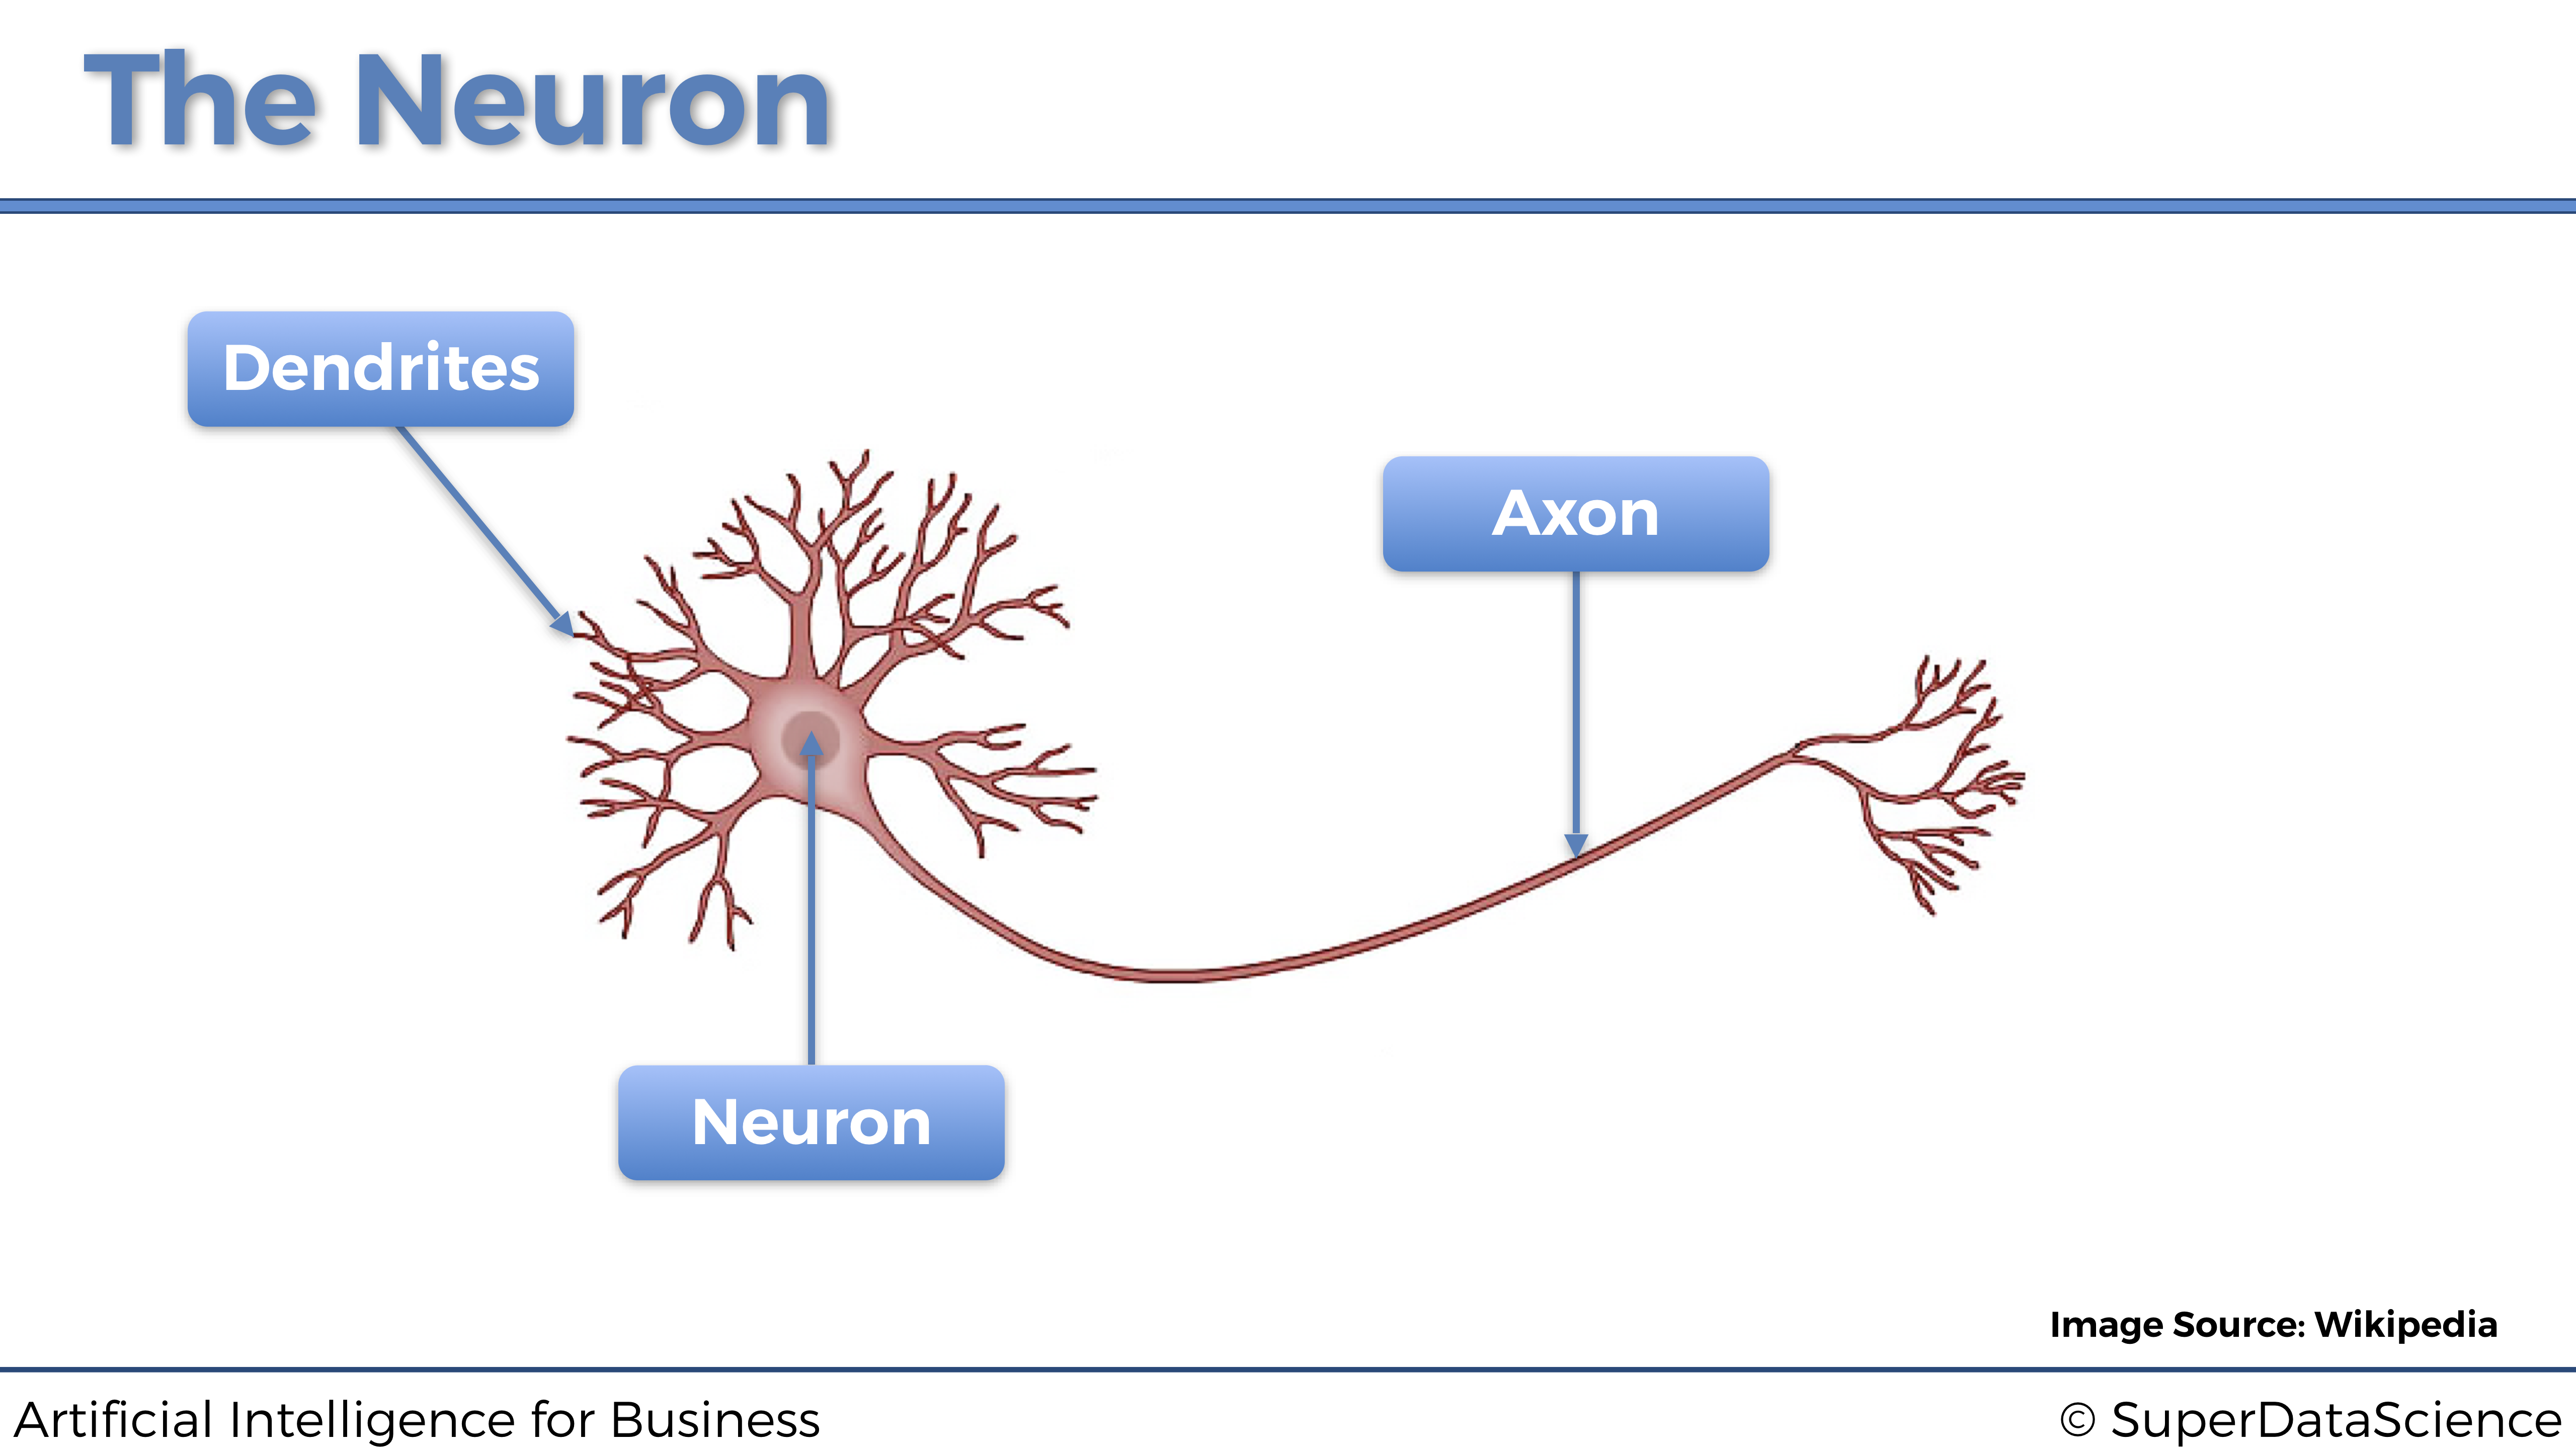
\includegraphics{Images/ANN_3.png}

Esto es una neurona. Esta neurona intercambia señales con sus neuronas vecinas. Las dendritas son los receptores de la señal y el axón es el transmisor de la señal. Aquí hay una imagen de cómo funciona todo conceptualmente:

\includegraphics{Images/ANN_4.png}

Podemos ver que las dendritas de la neurona están conectadas a los axones de otras neuronas por encima. Luego, la señal viaja por su axón y pasa a las dendritas de la siguiente neurona. Así es como están conectados y cómo funciona una neurona. Por lo tanto, ahora es el momento de pasar de la neurociencia a la tecnología.

Así es como se representa una neurona dentro de una red neuronal artificial:

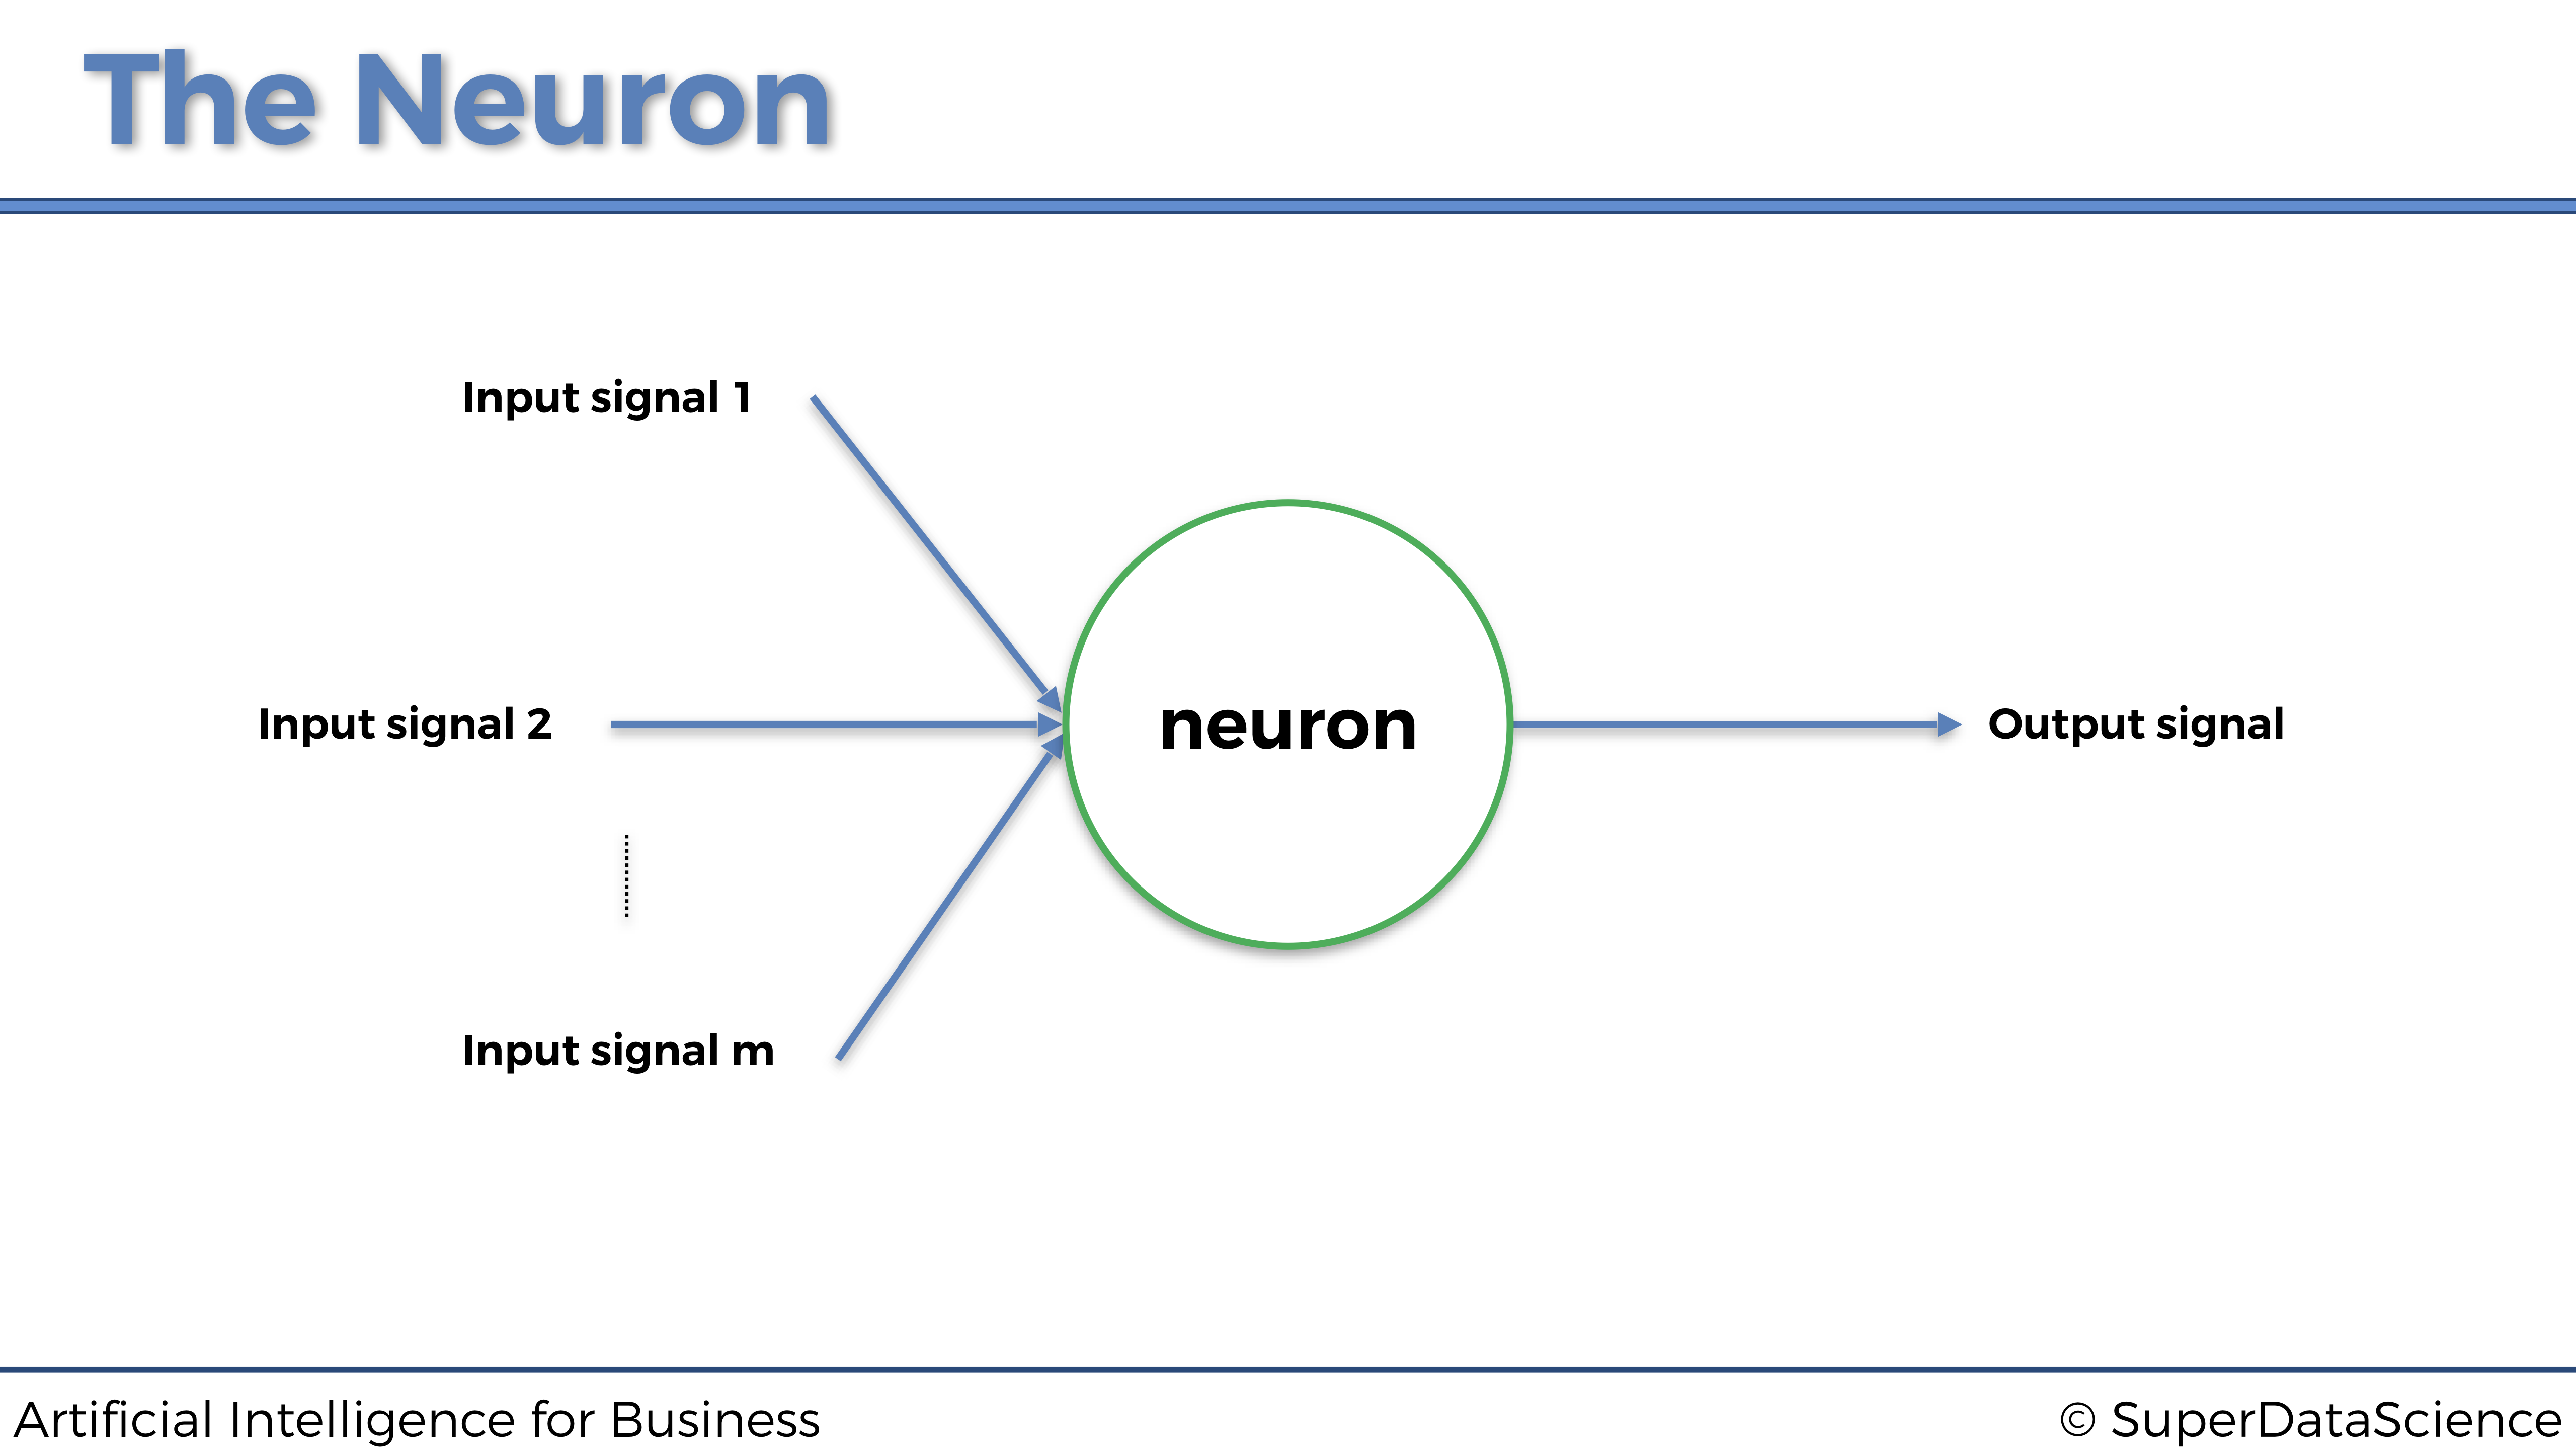
\includegraphics{Images/ANN_5.png}

Al igual que una neurona humana, recibe algunas señales de entrada y tiene una señal de salida. La flecha azul que conecta las señales de entrada a la neurona, y la neurona a la señal de salida, son como las sinapsis en la neurona humana. Pero aquí, en la neurona de la máquina, ¿cuáles serán exactamente estas señales de entrada y salida? Bueno, las señales de entrada serán las variables independientes escaladas que componen los estados del entorno, que recordemos en el caso práctico que nos ocupa son la temperatura del servidor, el número de usuarios y la velocidad de transmisión de datos, y la señal de salida será los valores de salida, que en el modelo de Deep Q-Learning son siempre los Q-Values. Por lo tanto, obtenemos la representación general de una neurona para ordenadores:

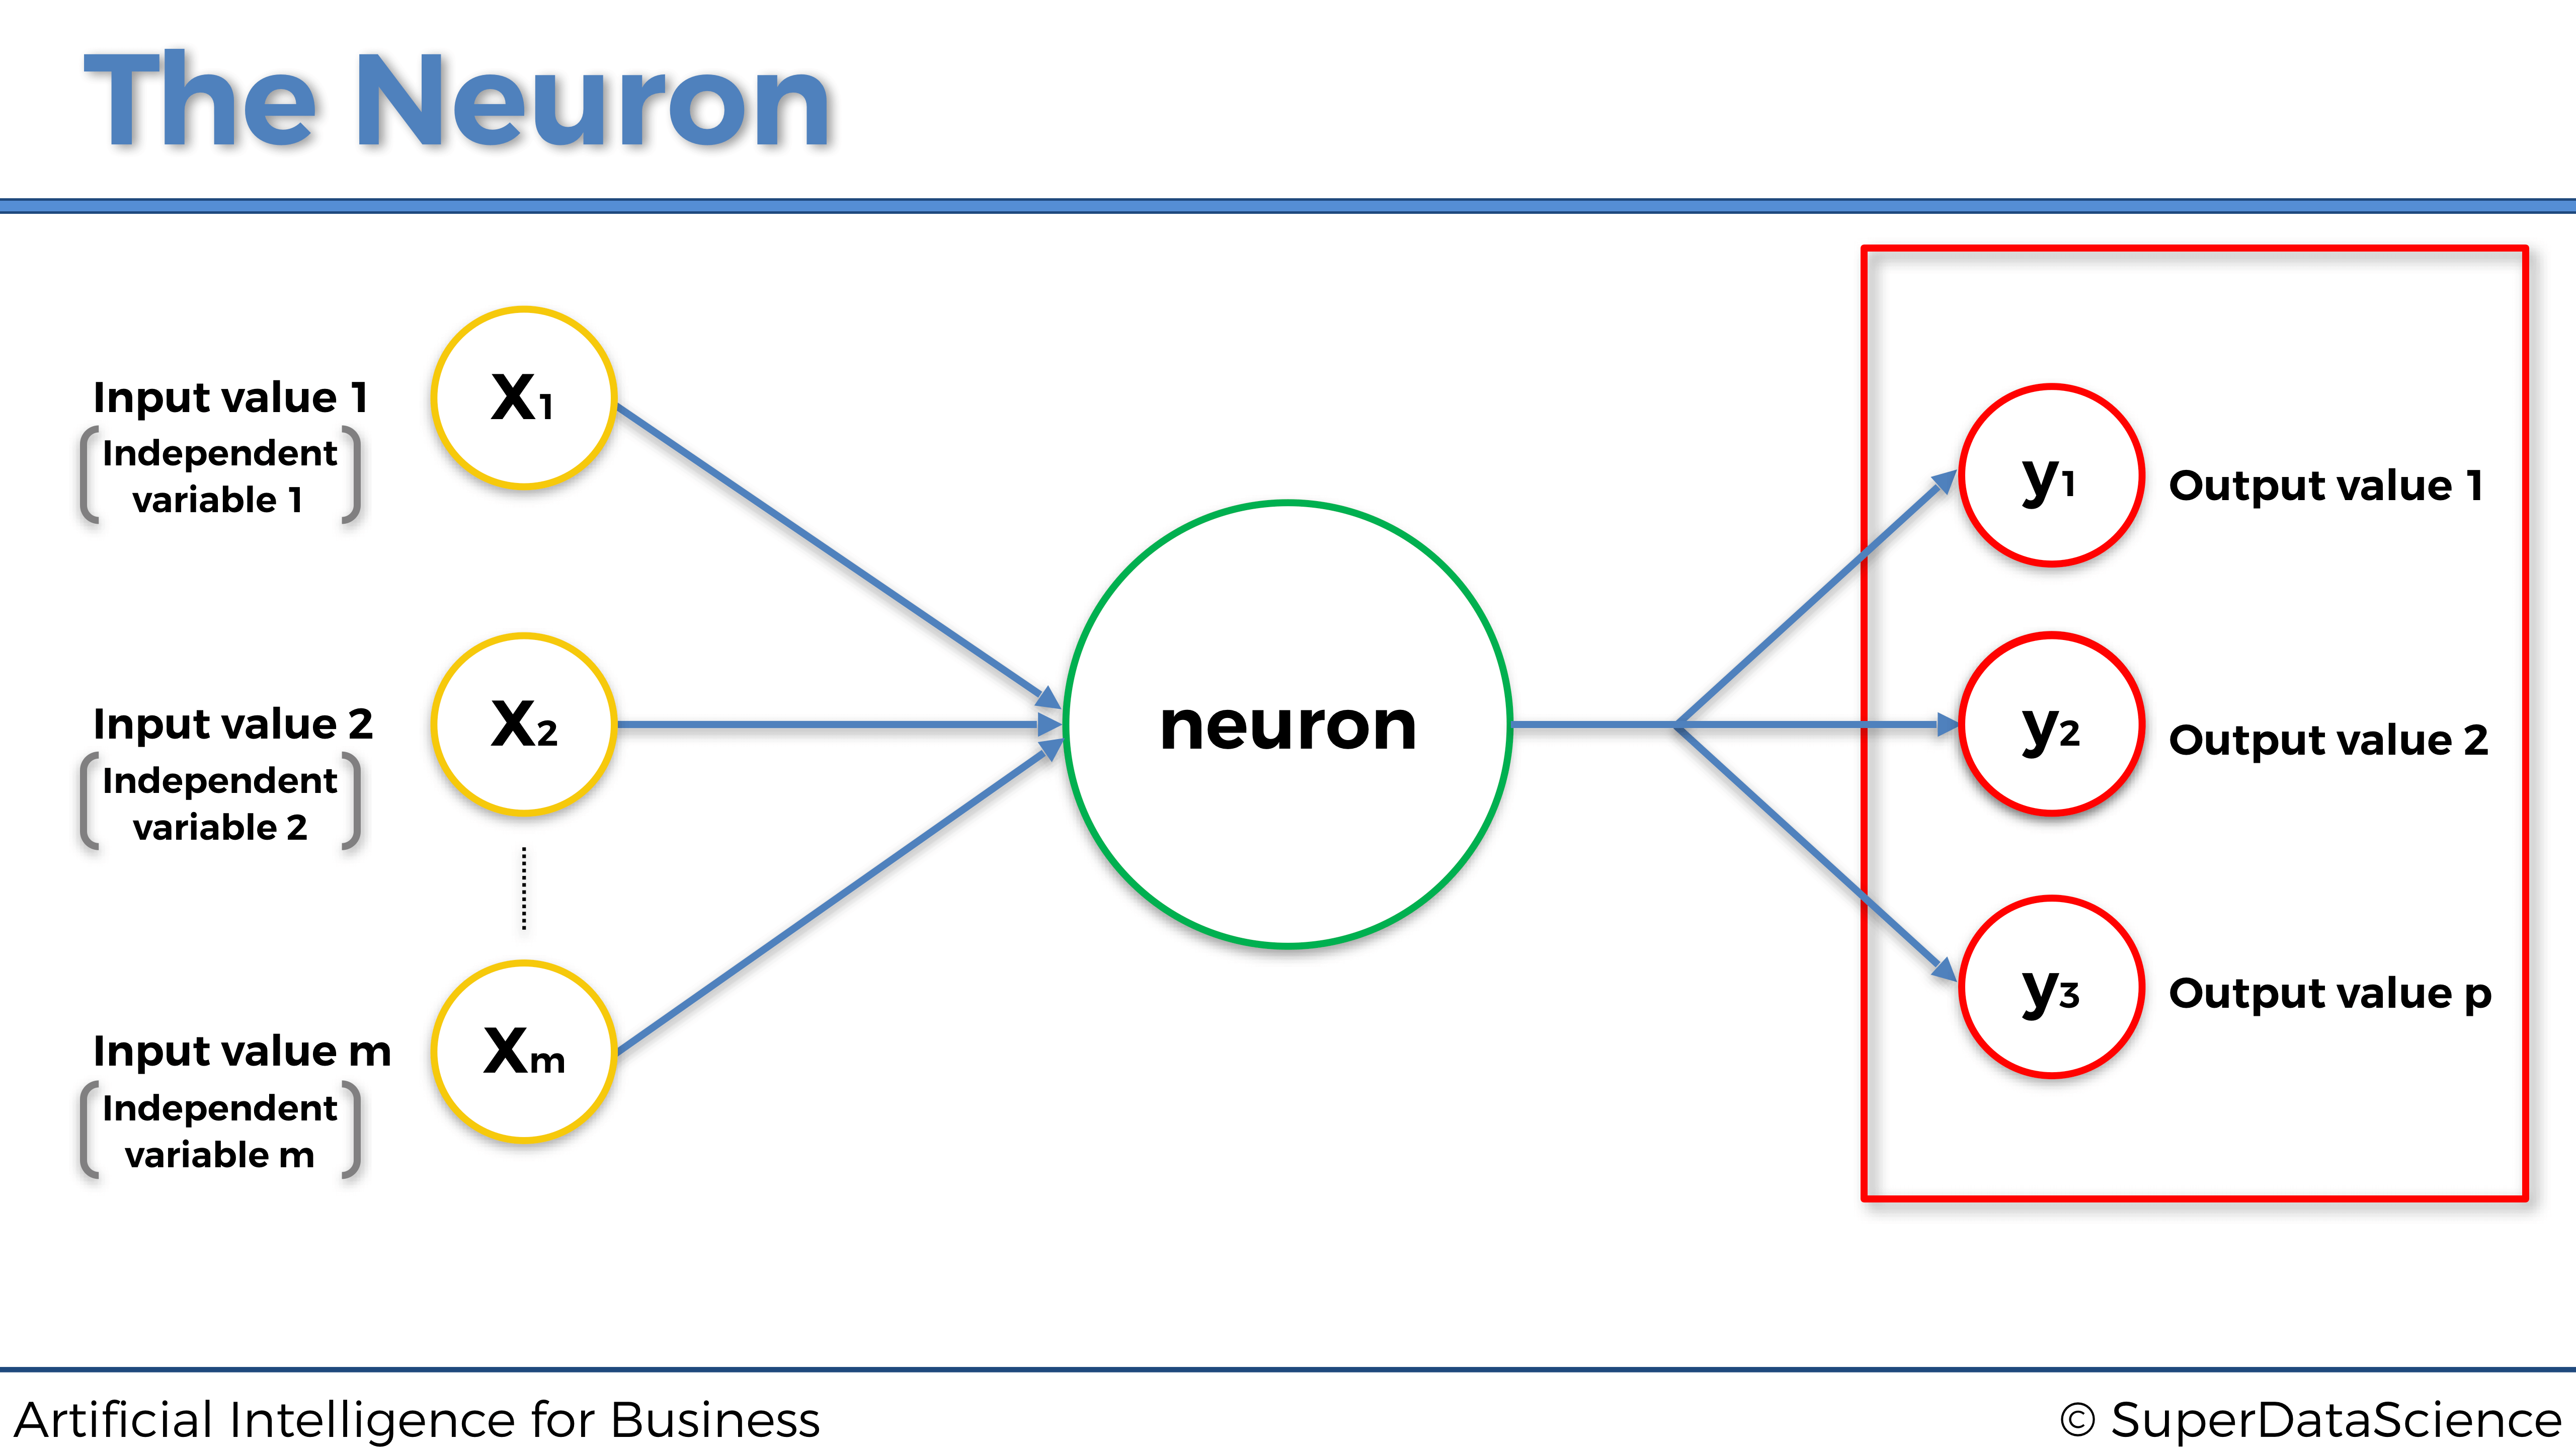
\includegraphics{Images/ANN_7.png}

Y ahora para terminar con la neurona, agreguemos los últimos elementos que faltan en esta representación, pero también los más importantes: los pesos. A cada sinapsis (flecha azul) se le atribuirá un peso. Cuanto mayor sea el peso, más fuerte será la señal a través de la sinapsis. Y lo que es fundamental entender es que, estos pesos, serán lo que la máquina actualizará y actualizará con el tiempo para mejorar las predicciones. Veámoslo en el gráfico anterior, para asegurarnos de que los visualizamos correctamente antes de seguir:

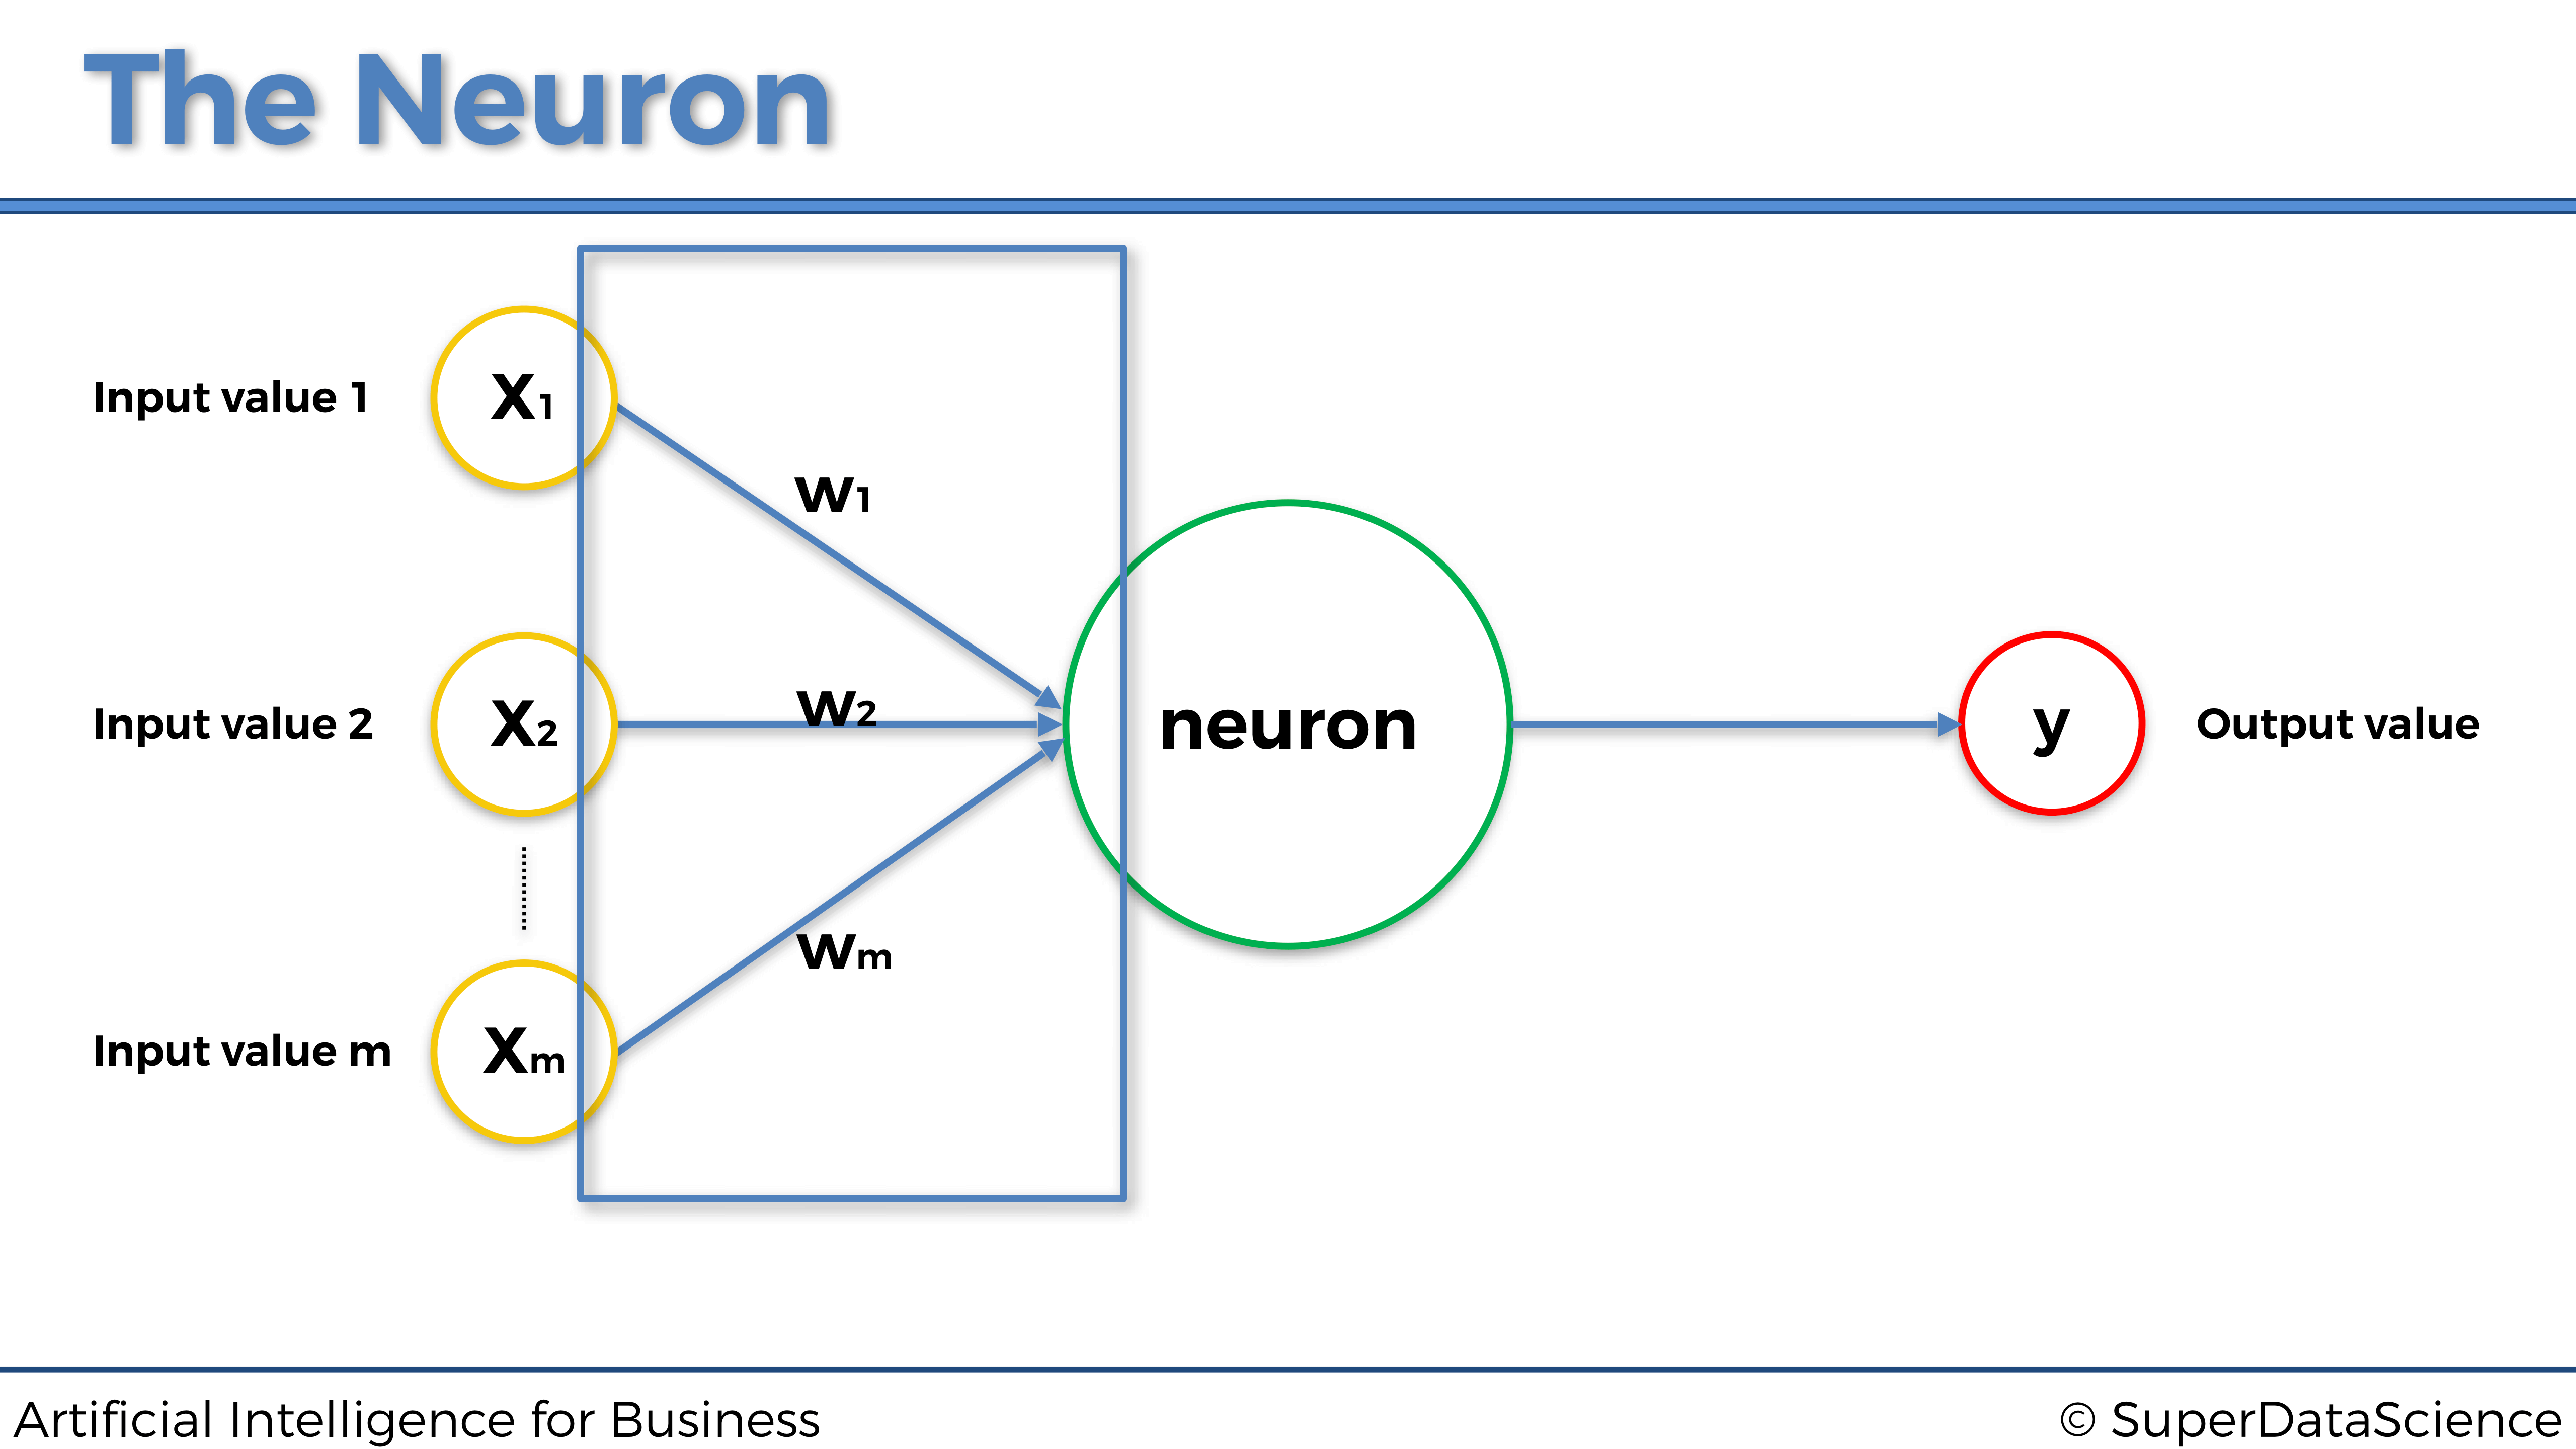
\includegraphics{Images/ANN_8.png}

\hypertarget{la-funciuxf3n-de-activaciuxf3n}{%
\subsection{La Función de Activación}\label{la-funciuxf3n-de-activaciuxf3n}}

La función de activación es la función \(\phi\) que opera dentro de la neurona, que tomará como entradas la combinación lineal de los valores de entrada multiplicados por sus pesos asociados, y sumados entre si y que devolverá el valor de salida:

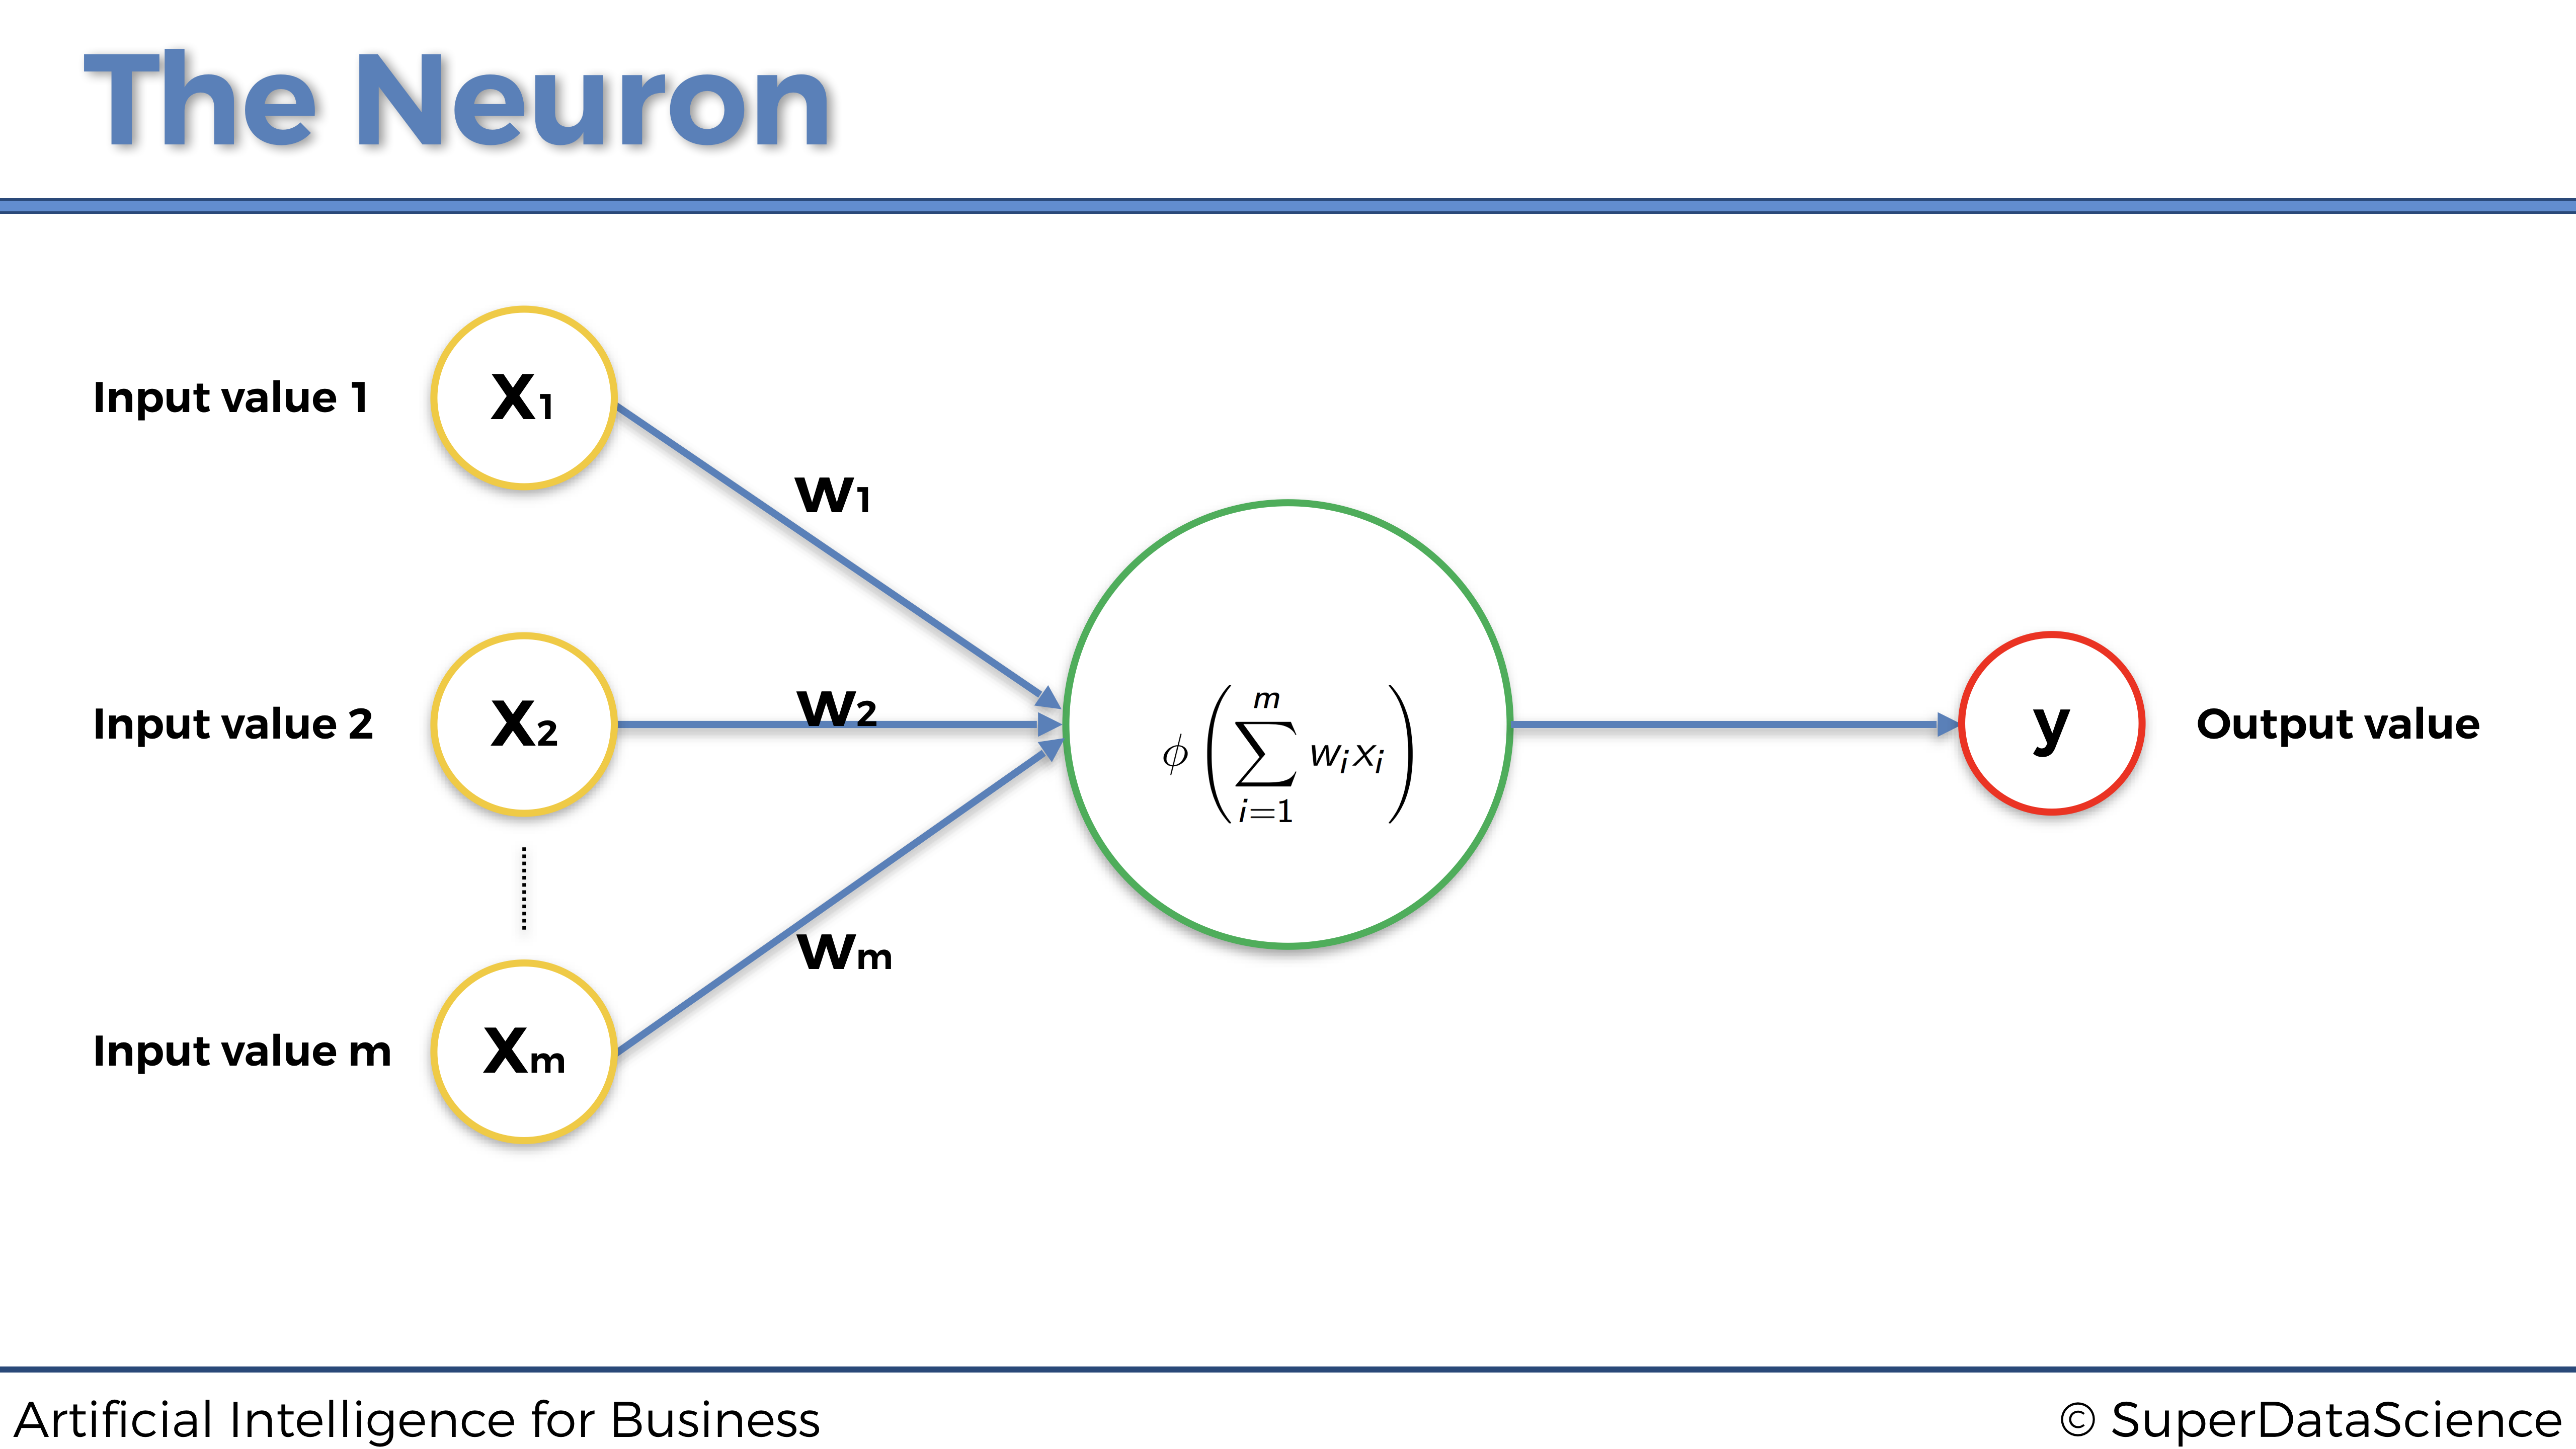
\includegraphics{Images/ANN_9.png}

calculado como

\[y = \phi\left( \sum_{i=1}^m w_i x_i \right)\]

¿Cuál será exactamente la función \(\phi\)?

Puede haber muchas de ellos, diferentes pero vamos a ver aquí los cuatro más usados, incluido, por supuesto, el que usamos en la Parte 2: Minimización de costos:

\begin{itemize}
\tightlist
\item
  La función de activación de umbral
\item
  La función de activación sigmoidea
\item
  La función de activación del rectificador
\item
  La función de activación de la tangente hiperbólica
\end{itemize}

Vamos a verlas todas una por una:

\hypertarget{la-funciuxf3n-de-activaciuxf3n-de-umbral}{%
\subsubsection{La función de activación de umbral}\label{la-funciuxf3n-de-activaciuxf3n-de-umbral}}

La función de activación de umbral, también llamada función escalón, se define simplemente como:

\[
\phi(x) =
    \begin{cases}
        1 \textrm{ si } x \ge 0 \\
        0 \textrm{ si } x < 0
    \end{cases}
\]

de modo que su representación gráfica es:

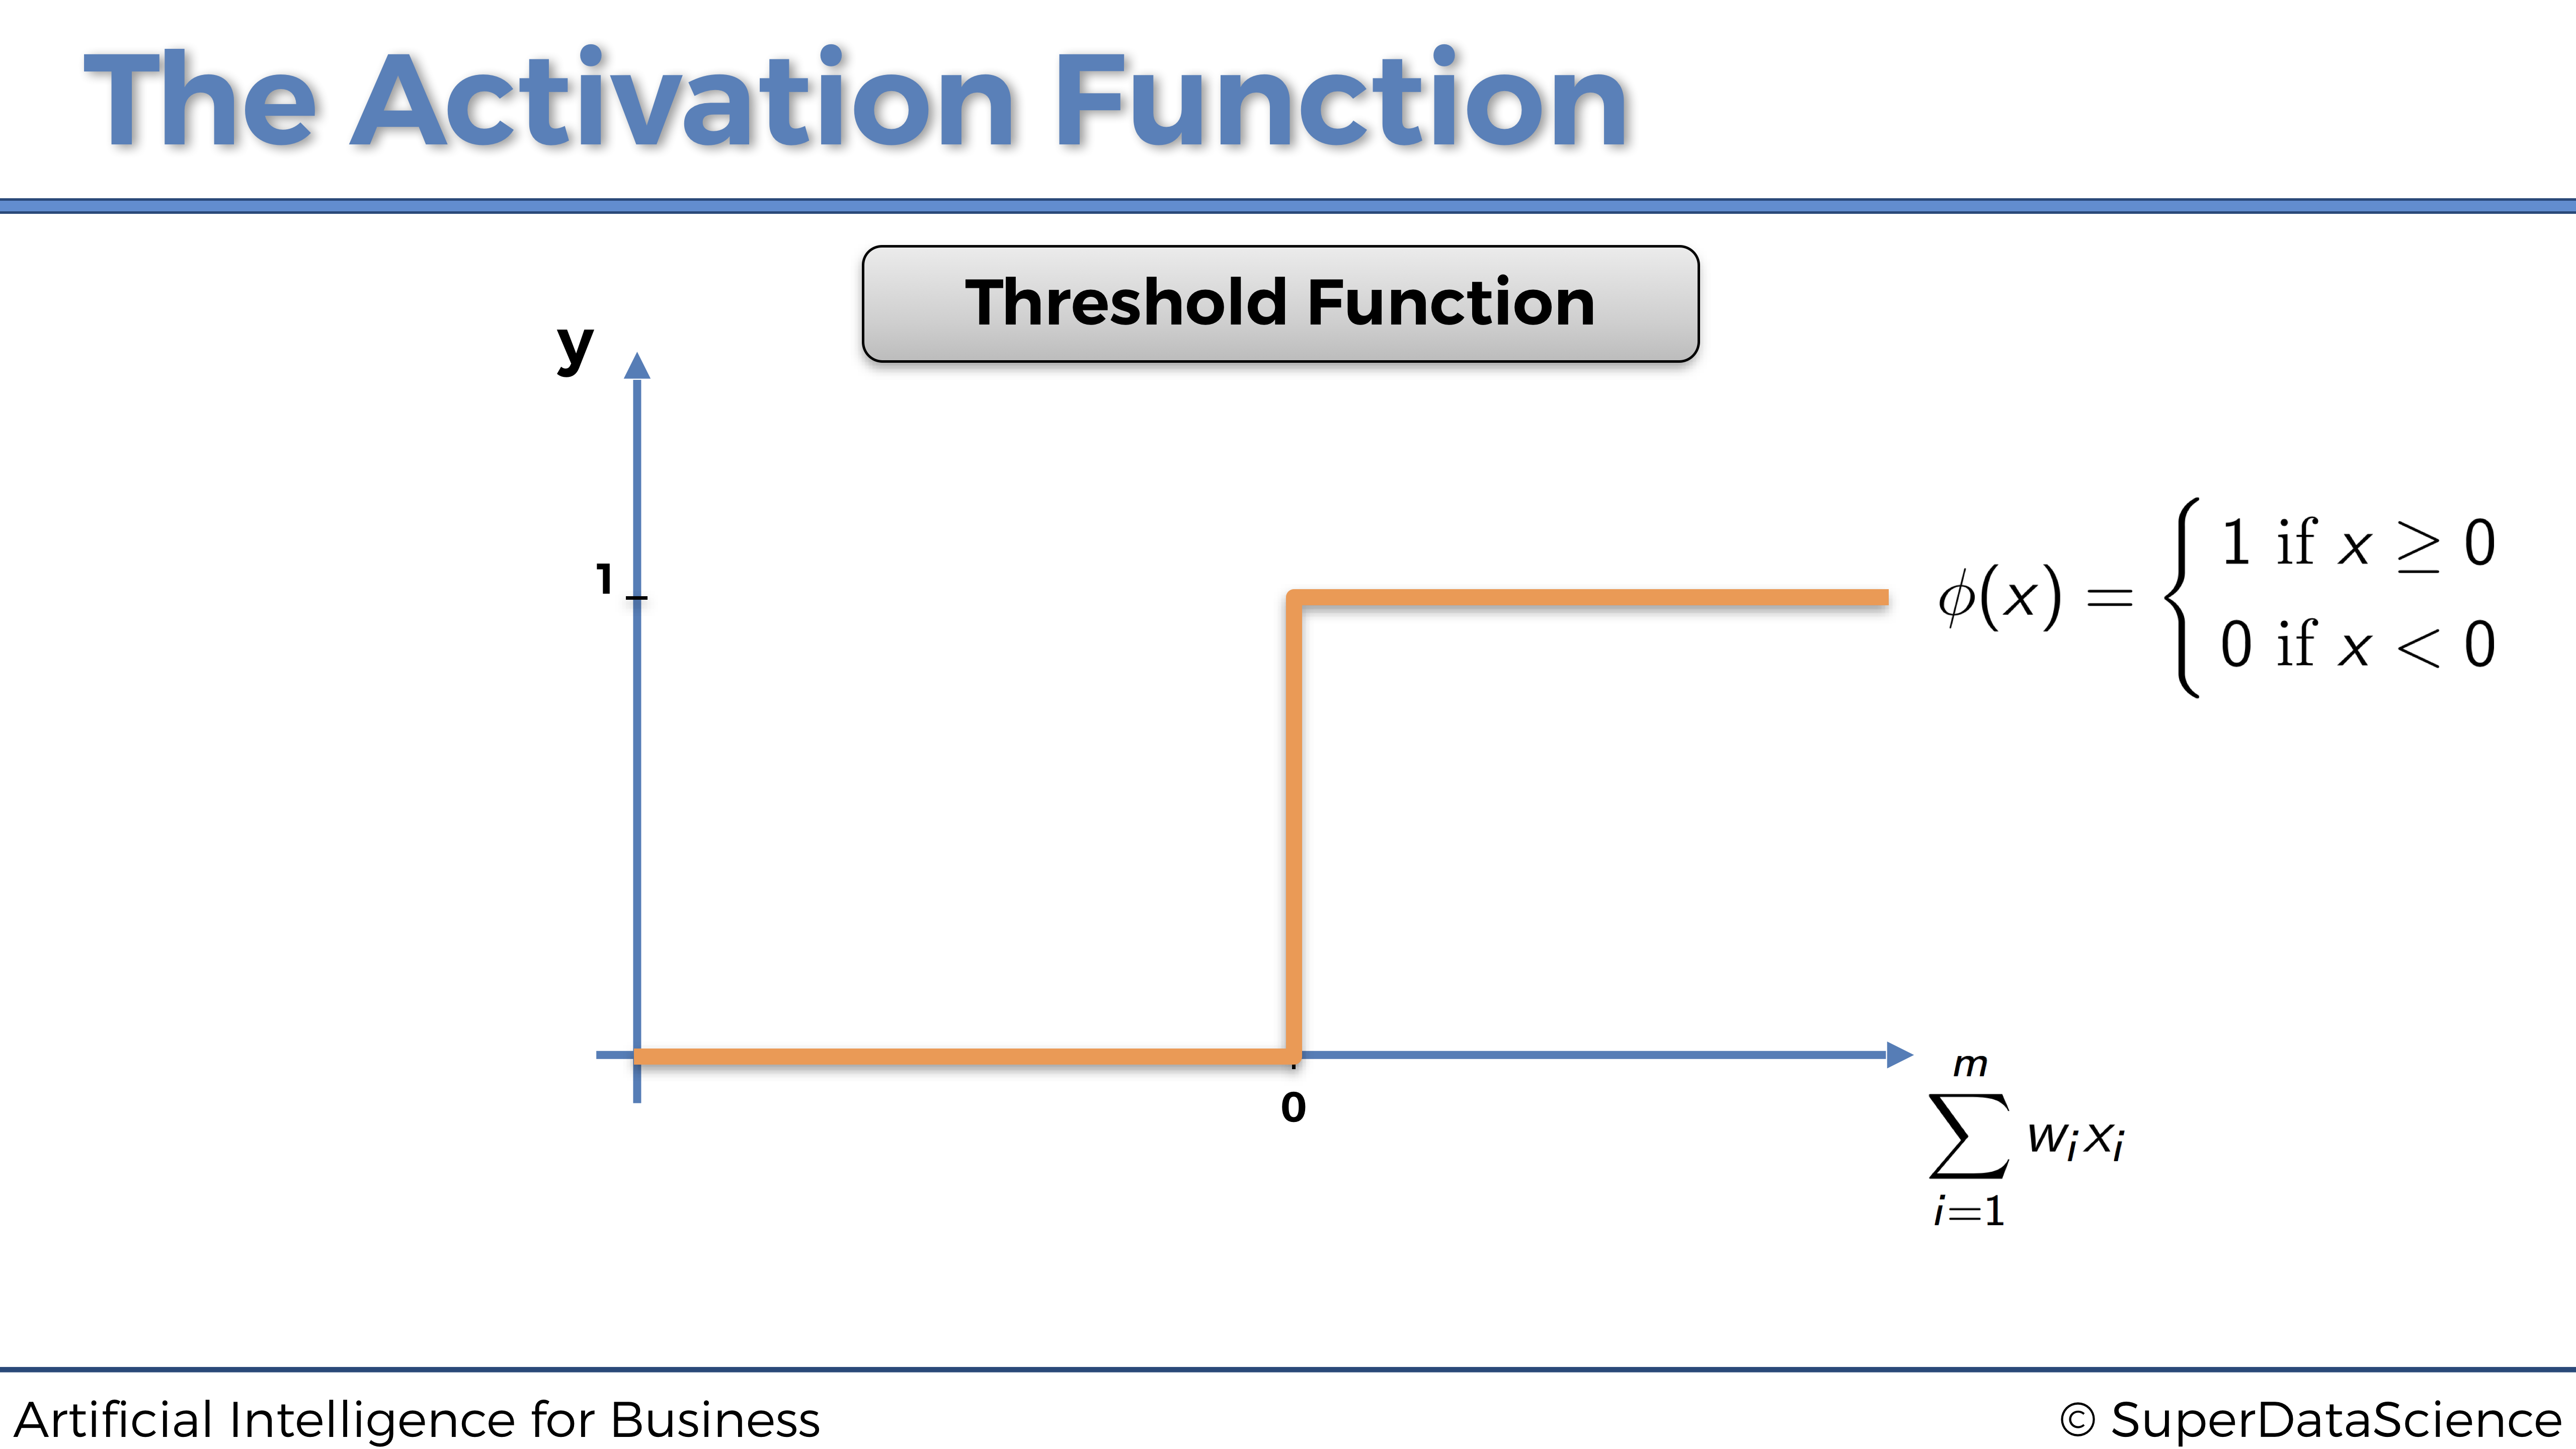
\includegraphics{Images/ANN_10.png}

Esto significa que la señal que pasa por la neurona será discontinua, y solo se activará si:

\[\sum_{i=1}^m w_i x_i \ge 0\]

\hypertarget{la-funciuxf3n-de-activaciuxf3n-sigmoidea}{%
\subsubsection{La función de activación sigmoidea}\label{la-funciuxf3n-de-activaciuxf3n-sigmoidea}}

Ahora echemos un vistazo a la siguiente función de activación: la función de activación sigmoidea.

La función de activación sigmoidea es la más efectiva y ampliamente utilizada en Redes Neuronales Artificiales, pero principalmente dentro de la última capa oculta (si se trata de una red neuronal profunda compuesta de varias capas ocultas) que pasa la señal hacia la capa de salida.

La función de activación sigmoidea se define como:

\[\phi(x) = \frac{1}{1+e^{-x}}\]

y da como resultado la siguiente representación gráfica:

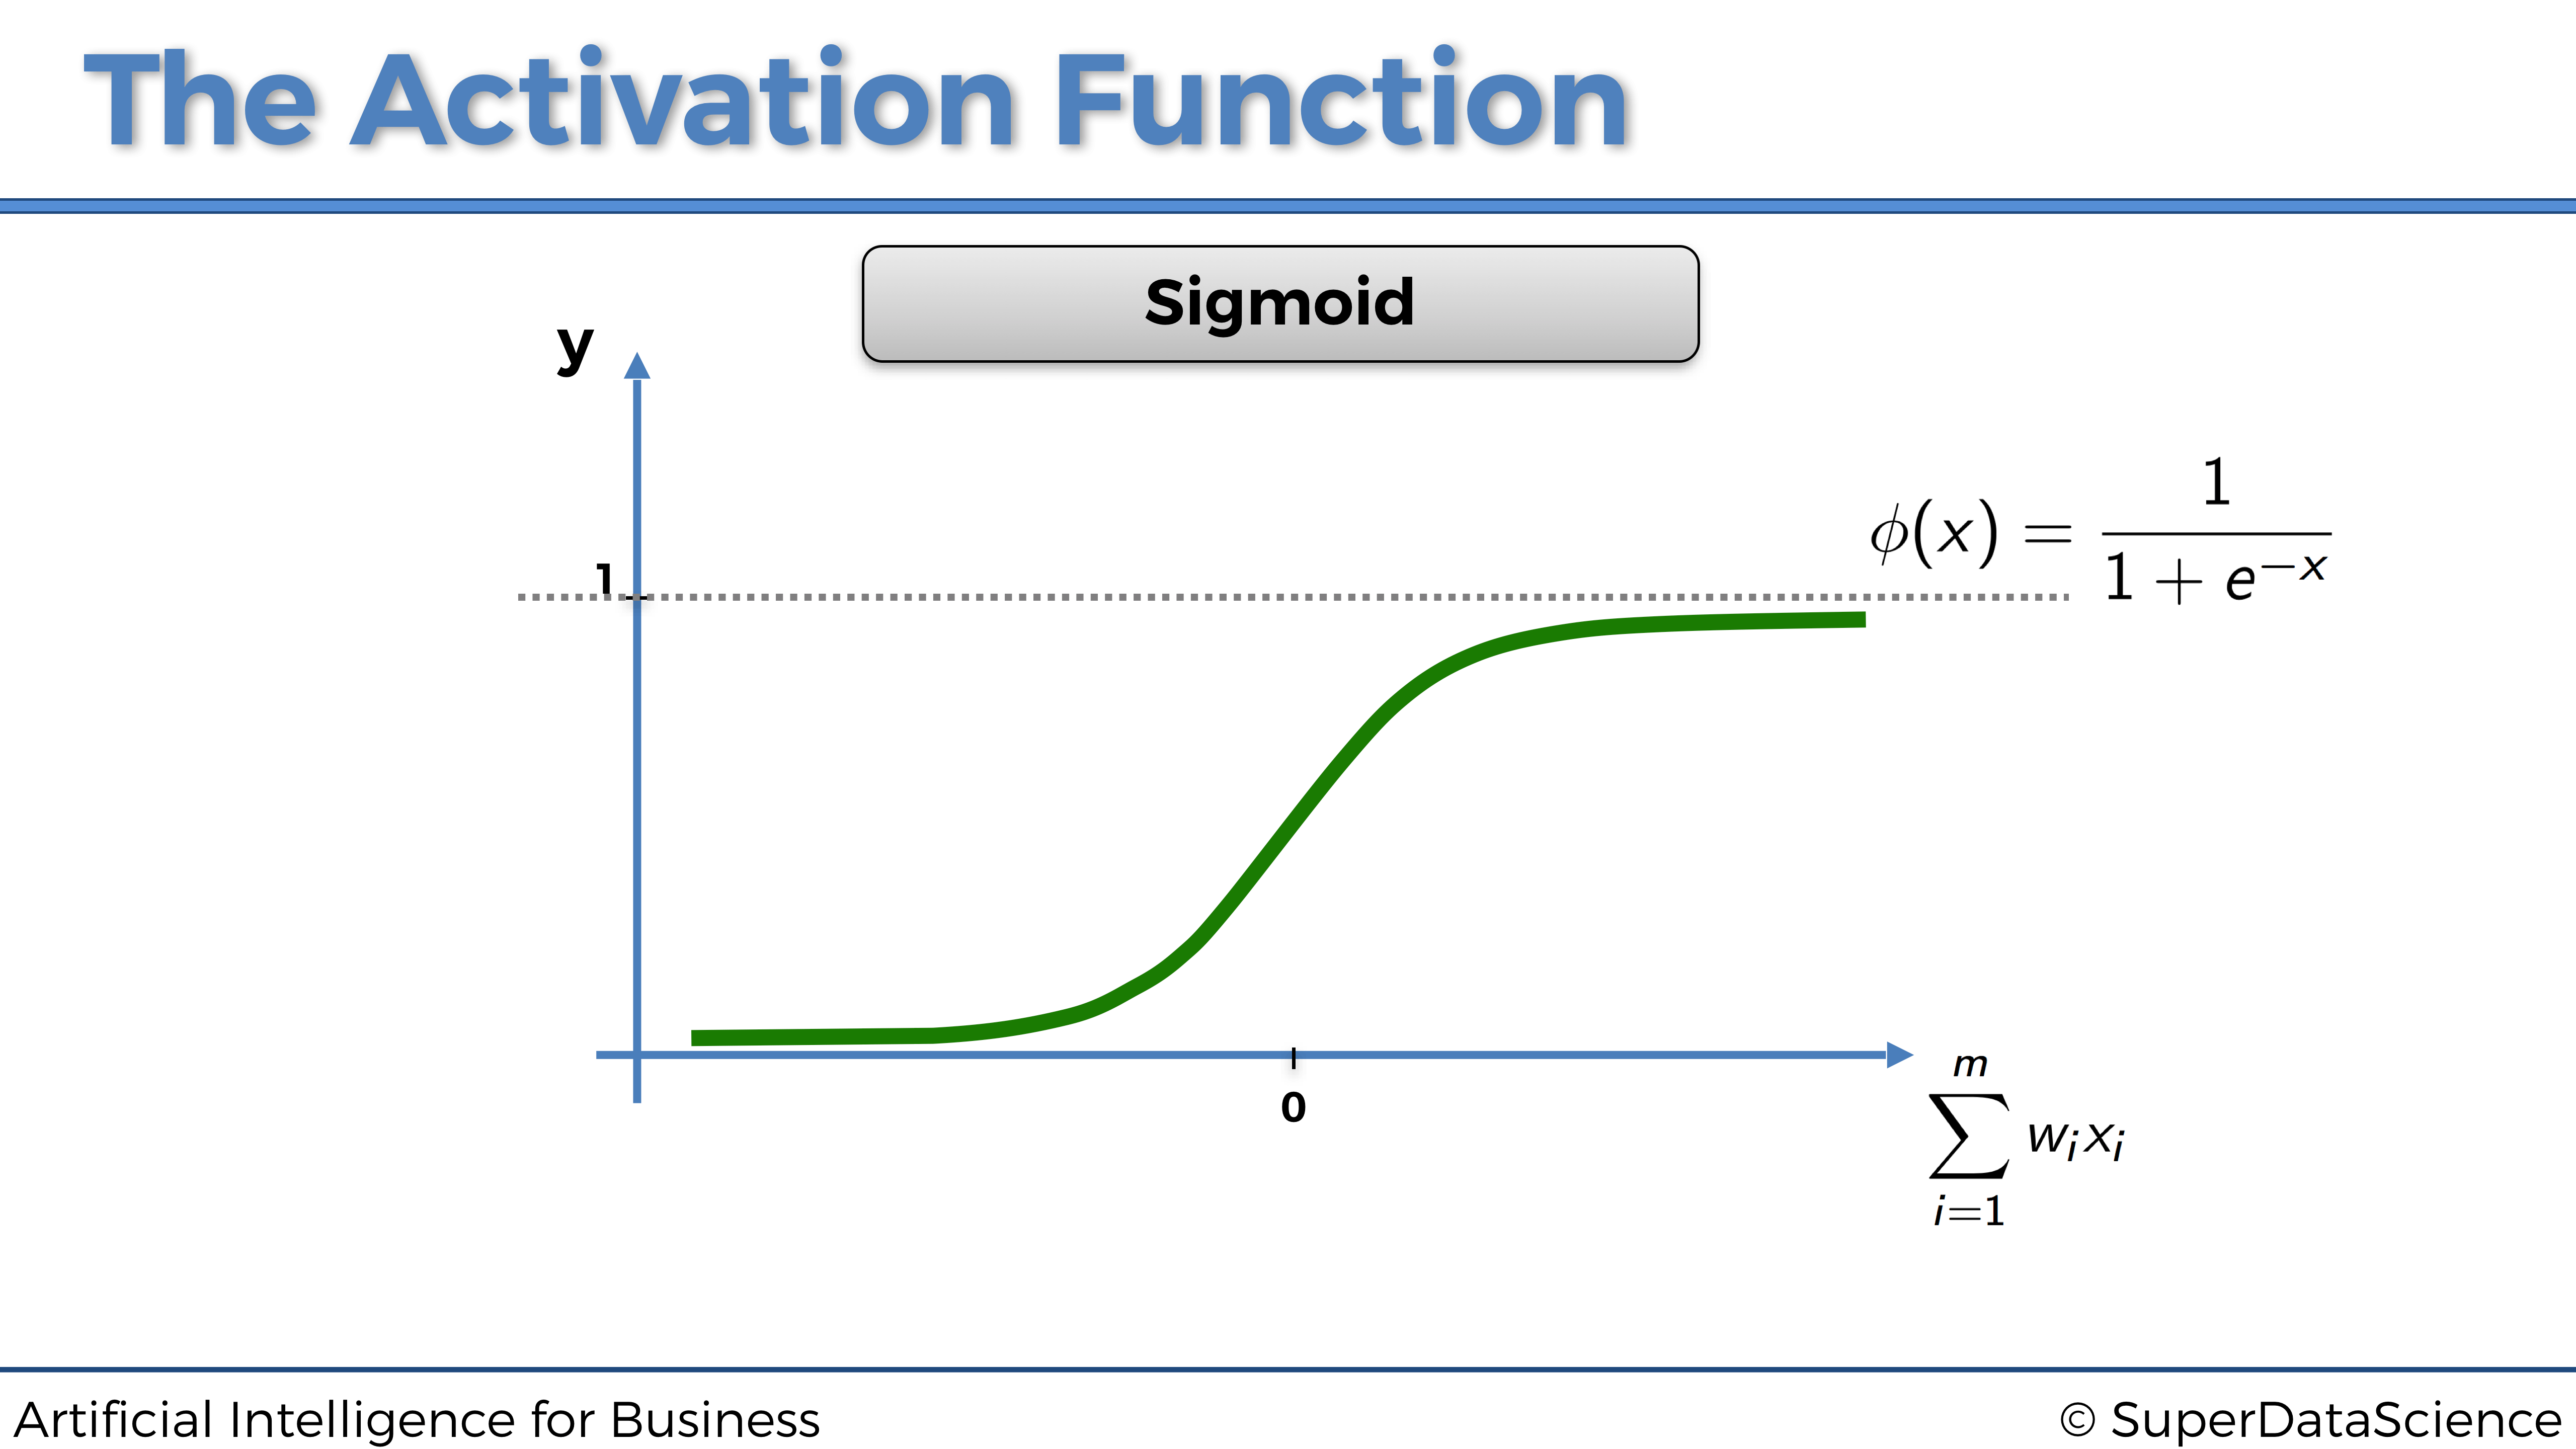
\includegraphics{Images/ANN_11.png}

Esto significa que la señal que pasa por la neurona será continua y siempre se activará. Y cuanto mayor sea \(\sum_{i = 1}^m w_i x_i\), más fuerte será esa señal.

\hypertarget{la-funciuxf3n-de-activaciuxf3n-rectificadora}{%
\subsubsection{La función de activación rectificadora}\label{la-funciuxf3n-de-activaciuxf3n-rectificadora}}

Ahora echemos un vistazo a otra función de activación ampliamente utilizada: la función de activación rectificadora.

La solemos encontrar en la mayoría de las redes neuronales \textbf{profundas}, pero sobretodo dentro de las capas ocultas, a diferencia de la función sigmoidea que se usa más bien para la capa de salida.

La función de activación rectificadora se define simplemente como:

\[\phi(x) = \max(x,0)\]

de modo que nos da lugar a la siguiente representación gráfica:

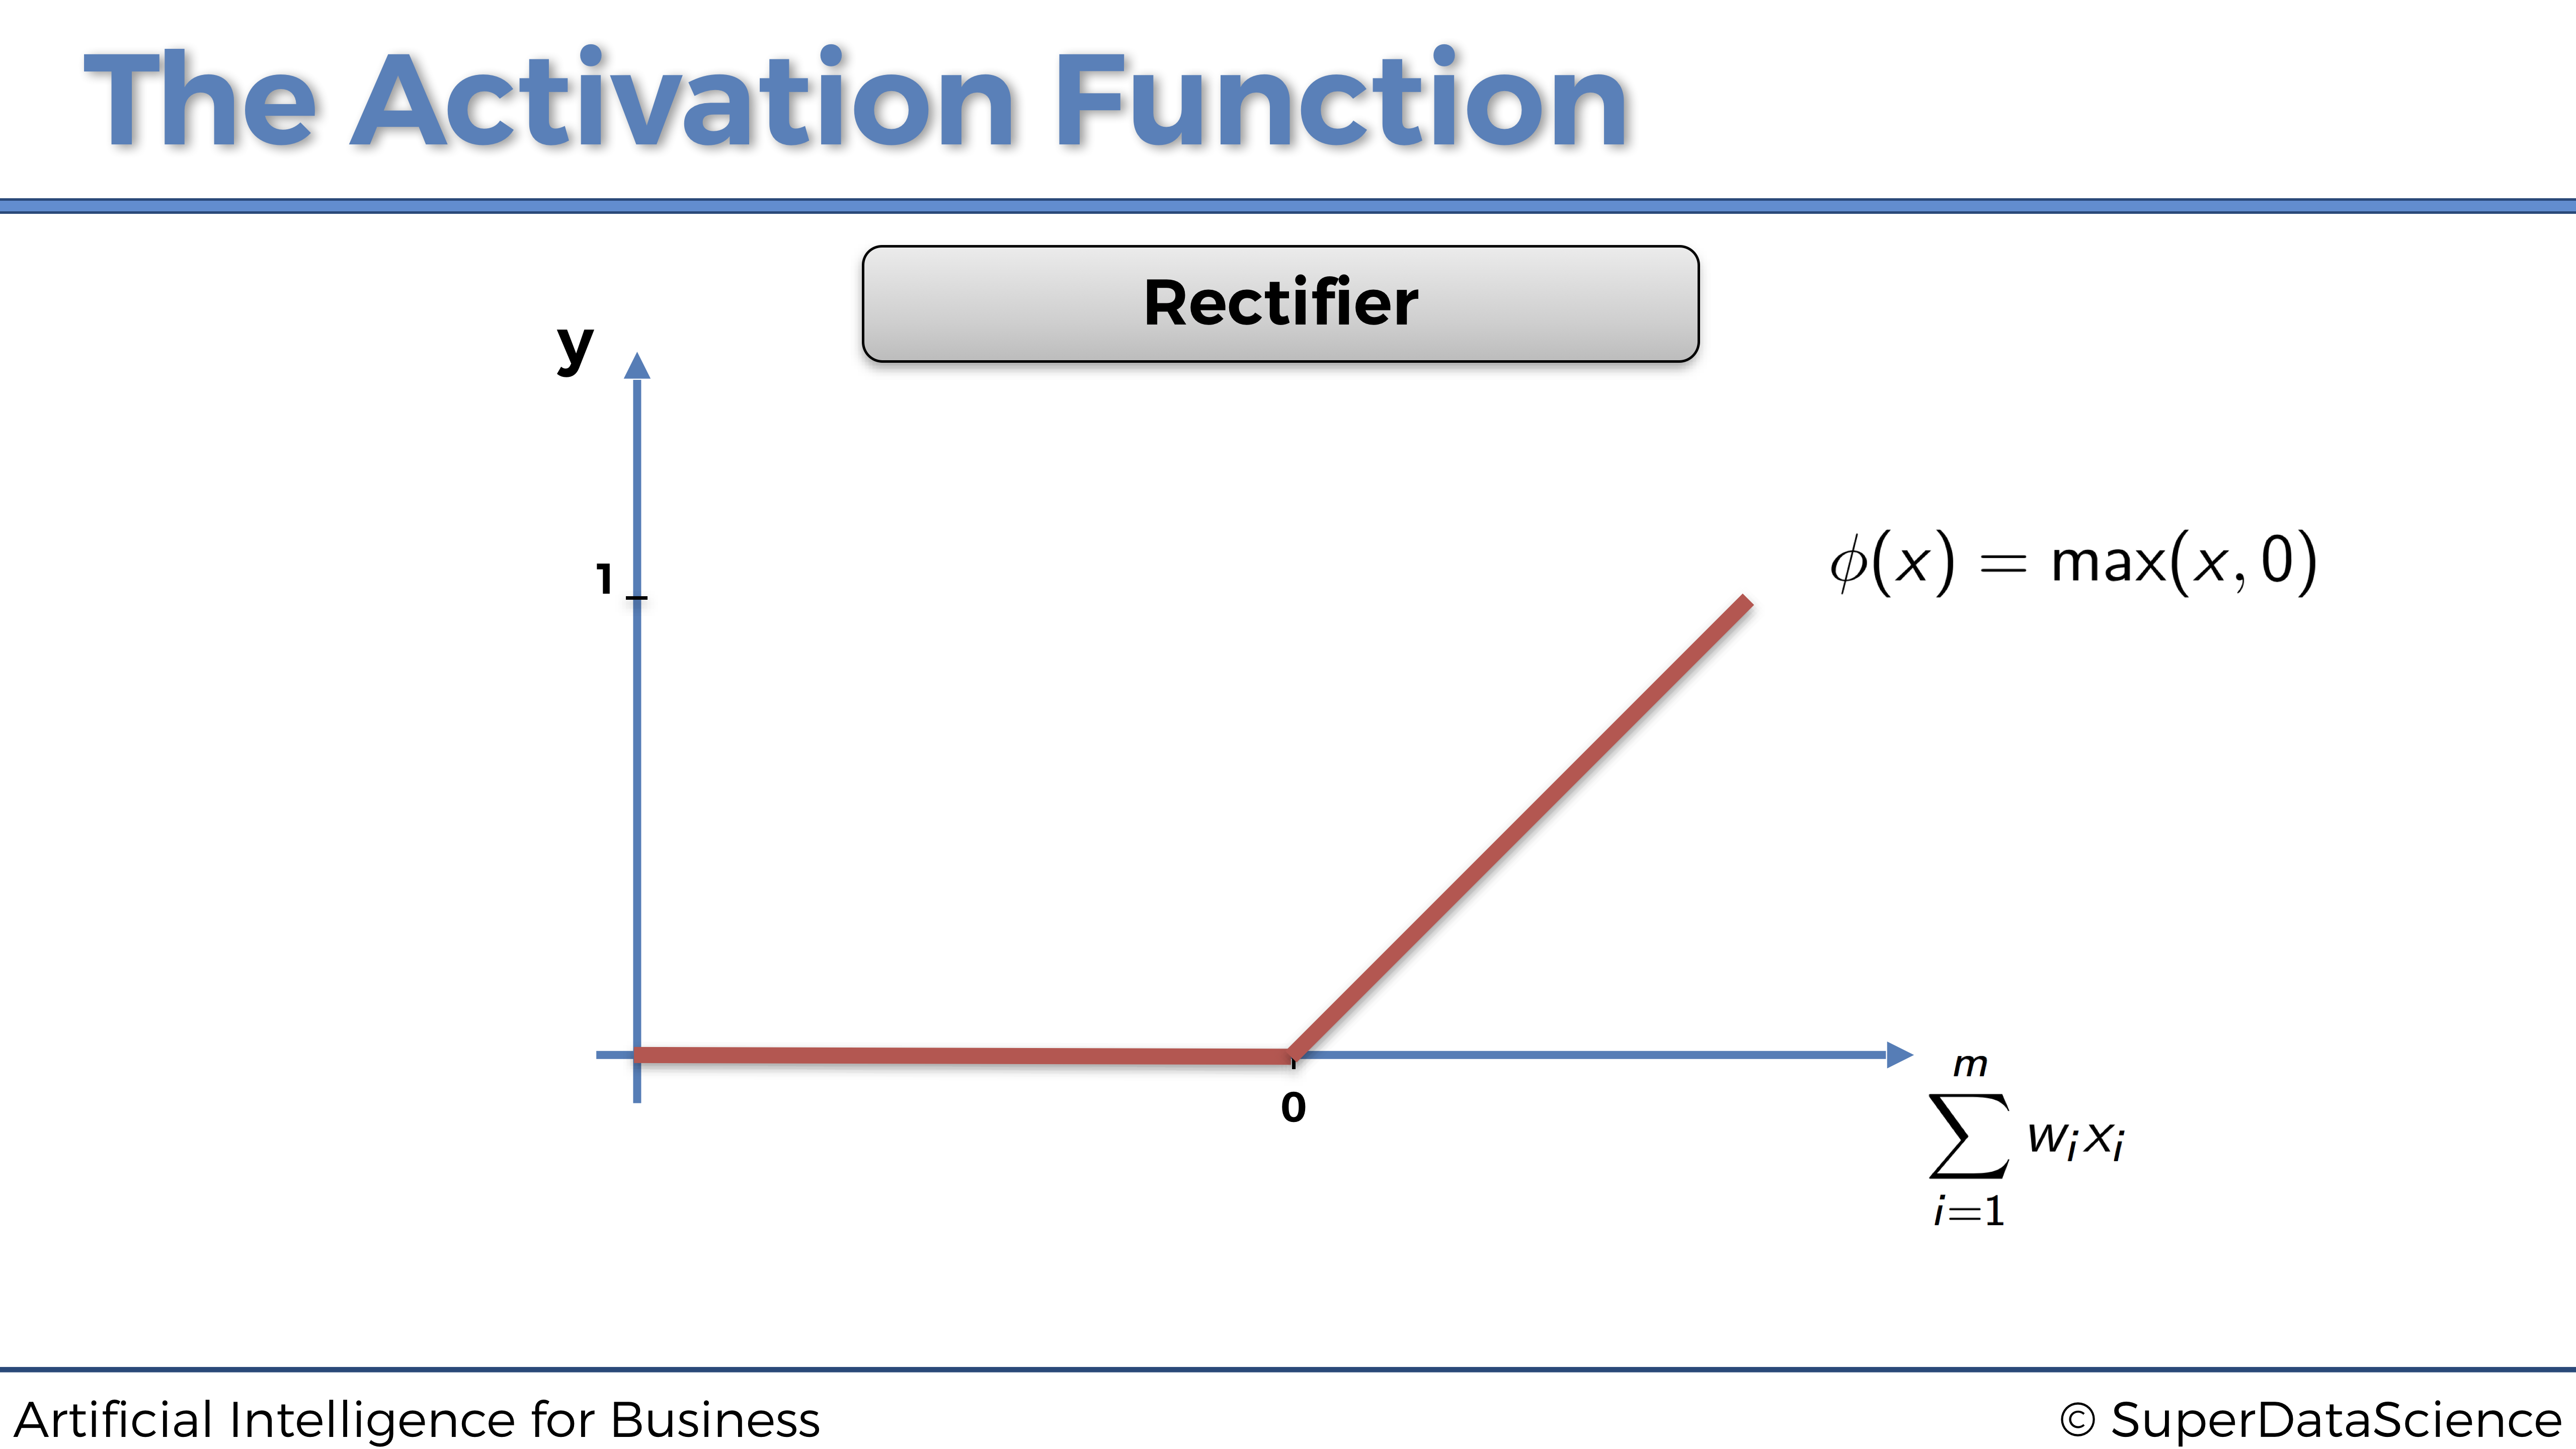
\includegraphics{Images/ANN_12.png}

Esto significa que la señal que pasa por la neurona será continua y solo se activará si:

\[\sum_{i=1}^m w_i x_i \ge 0\]

Y como mayor sea \(\sum_{i=1}^m w_i x_i\) por encima de 0, más fuerte será la señal transmitida.

\hypertarget{la-funciuxf3n-de-activaciuxf3n-de-la-tangente-hiperbuxf3lica}{%
\subsubsection{La función de activación de la tangente hiperbólica}\label{la-funciuxf3n-de-activaciuxf3n-de-la-tangente-hiperbuxf3lica}}

Ahora echemos un vistazo a la siguiente función de activación: la función de activación de la tangente hiperbólica.

La función de activación de la tangente hiperbólica es la menos utilizada, aunque a veces puede ser una opción más relevante en algunas Redes Neuronales Artificiales, especialmente cuando las entradas están estandarizadas.

La función de activación de la tangente hiperbólica se define por lo siguiente:

\[\phi(x) = \frac{1-e^{-2x}}{1+e^{-2x}}\]

de modo que da lugar a la siguiente:

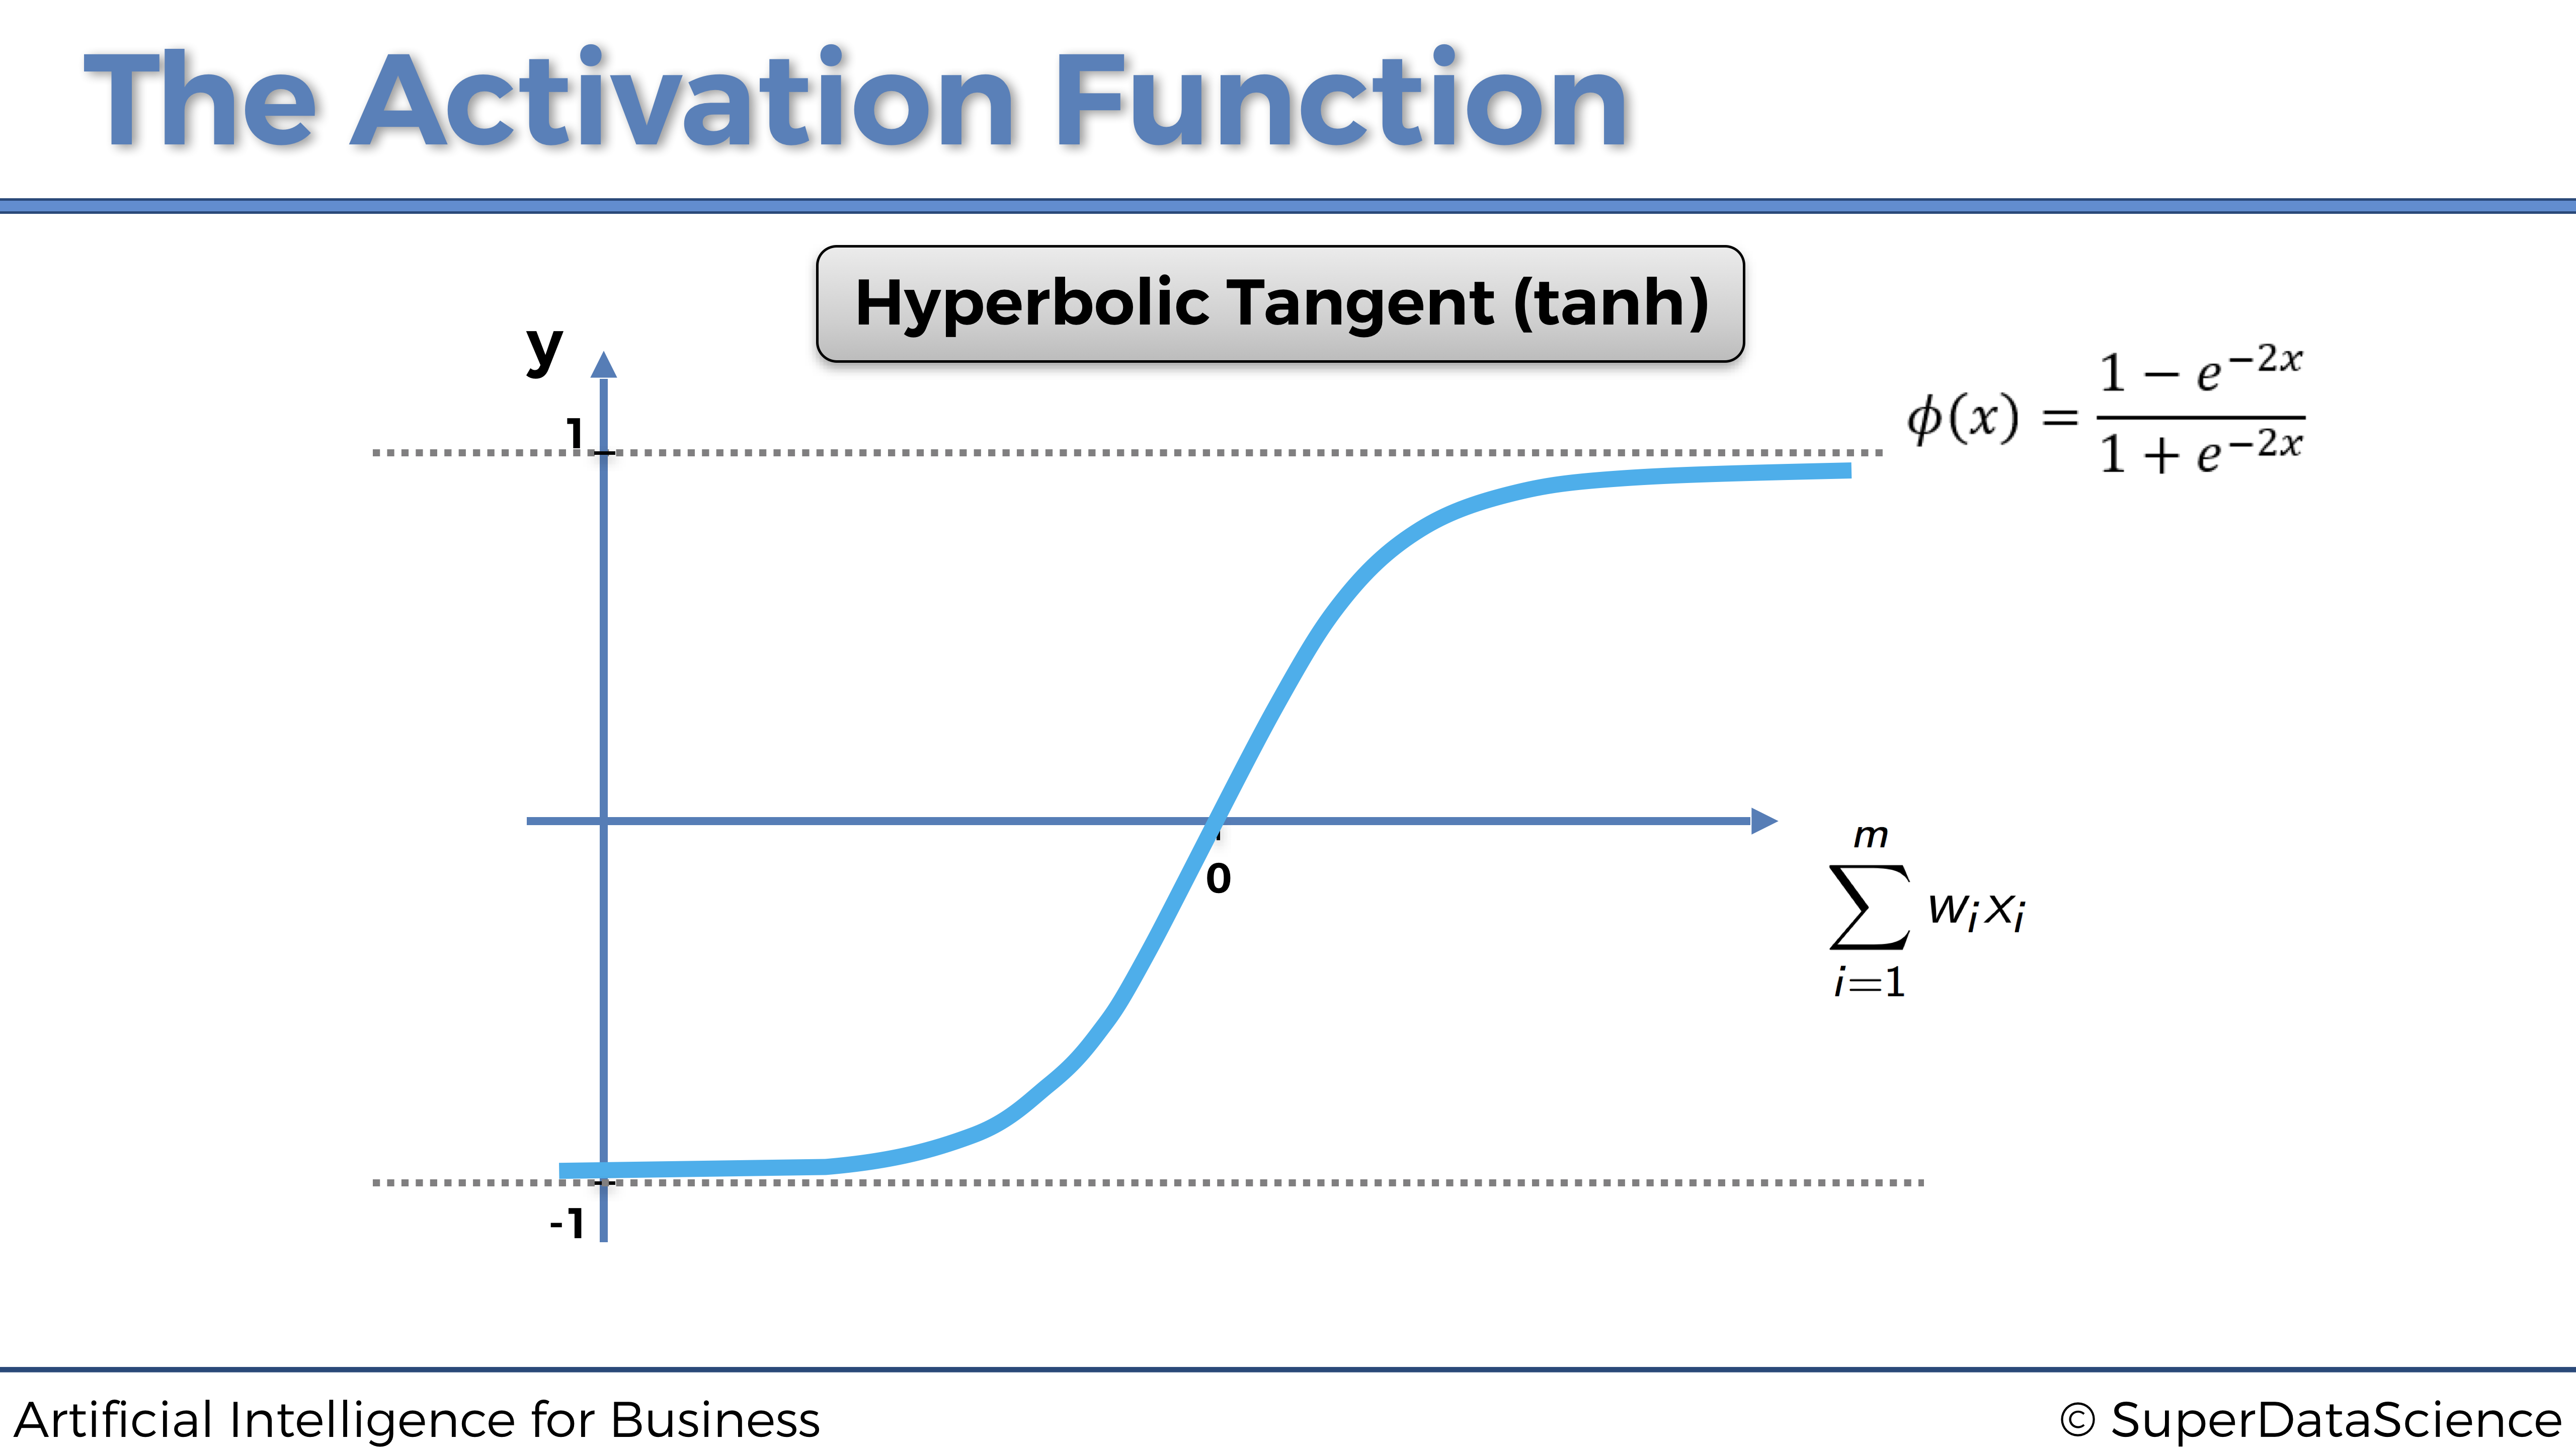
\includegraphics{Images/ANN_13.png}

Esto significa que la señal que pasa por la neurona será continua y siempre se activará. Cuanto más el valor de \(\sum_{i = 1}^m w_i x_i\) está por encima de 0, más fuerte será esa señal. Cuanto menos el valor de \(\sum_{i = 1}^m w_i x_i\) está por debajo de 0, más débil será esa señal.

Eso plantea la pregunta: ¿qué función de activación deberíamos elegir? O también la pregunta que más me suelen hacer, ¿cómo sabemos cuál elegir?

Buenas noticias, la respuesta es simple, y vamos a verlo dentro de un pequeño algoritmo.

Eso realmente depende de lo que se devuelve como la variable dependiente. Si es un resultado binario 0 o 1, entonces una mejor opción sería la función de activación del umbral. Si lo que desea que se devuelva es la probabilidad de que la variable dependiente sea 1, entonces una opción excelente es la función de activación sigmoidea, ya que su curva sigmoidea se ajusta perfectamente a las probabilidades del modelo.

Aquí está este pequeño detalle resaltado en esta imagen:

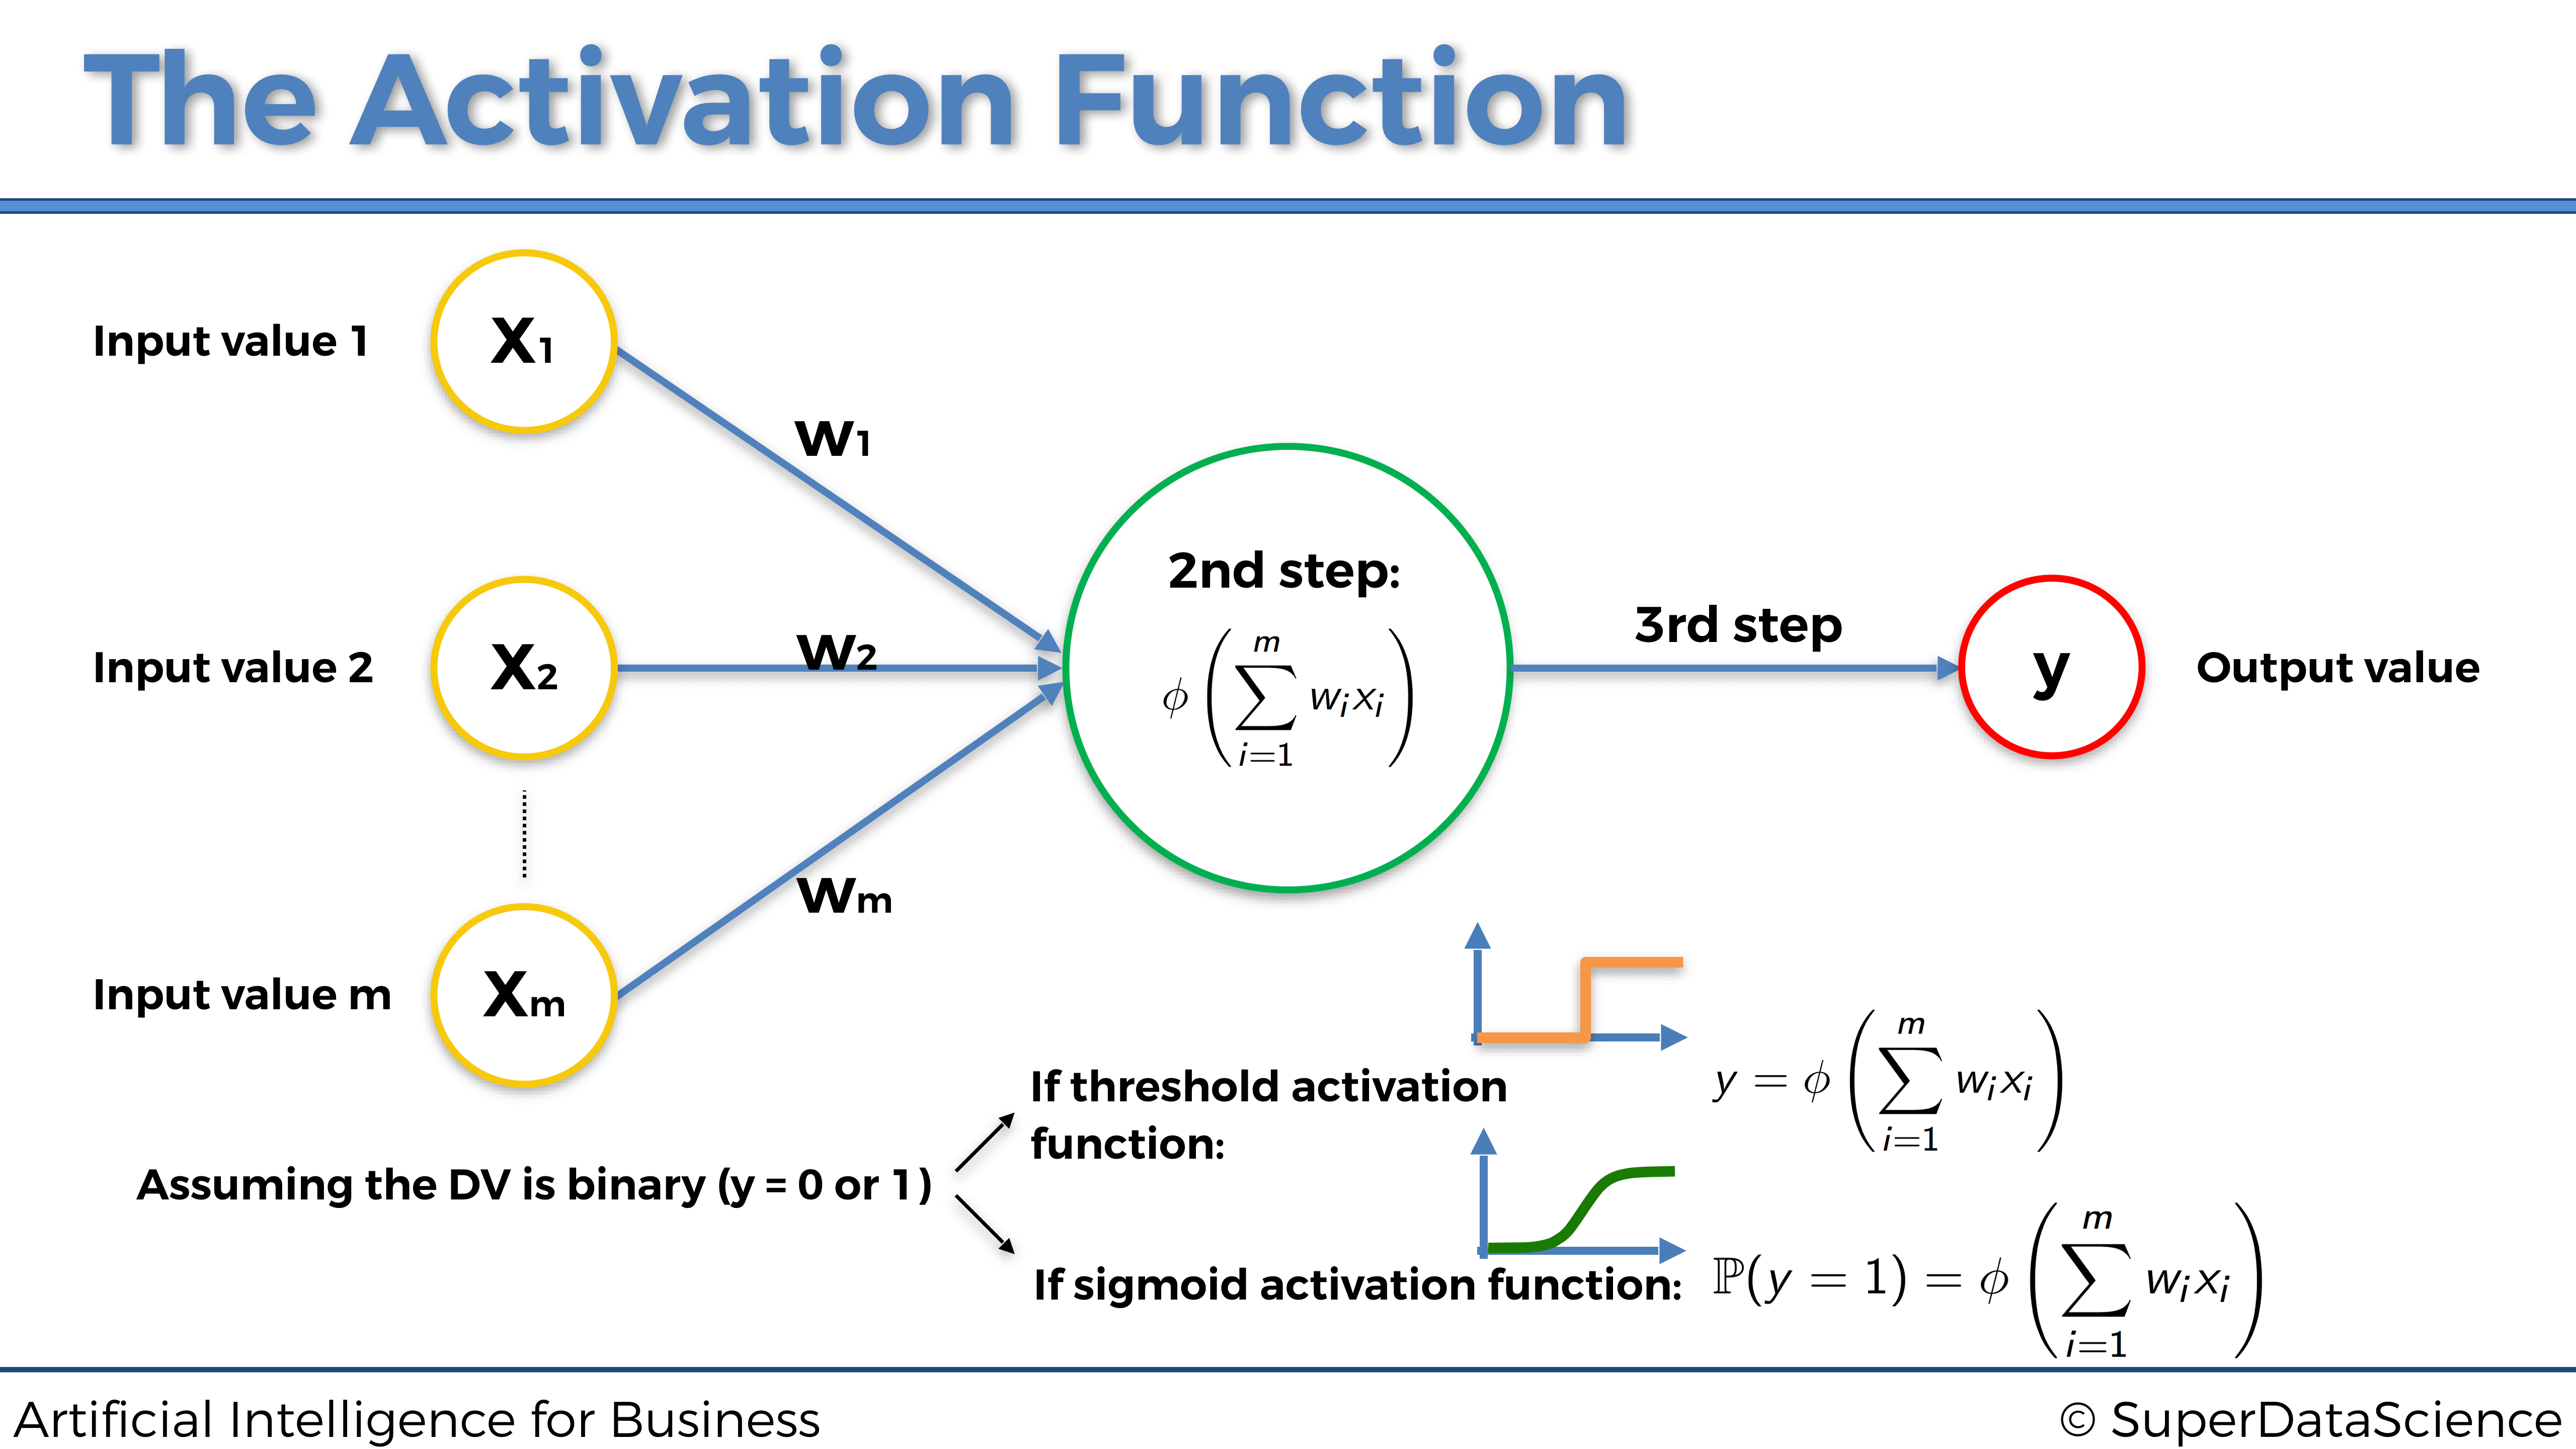
\includegraphics{Images/ANN_14.png}

Pero entonces, ¿cuándo debo usar las otras dos funciones de activación, es decir, la función de activación del rectificador y la función de activación de la tangente hiperbólica?

Nuevamente, las funciones de activación rectificador y tangente hiperbólica deben usarse dentro de las capas ocultas de una Red neuronal profunda (con más de una capa oculta), excepto en la última capa oculta que conduce a la capa de salida para la cual se recomienda usar un función de activación sigmoidea.

Recapitulemos esto nuevamente dentro de la siguiente imagen:

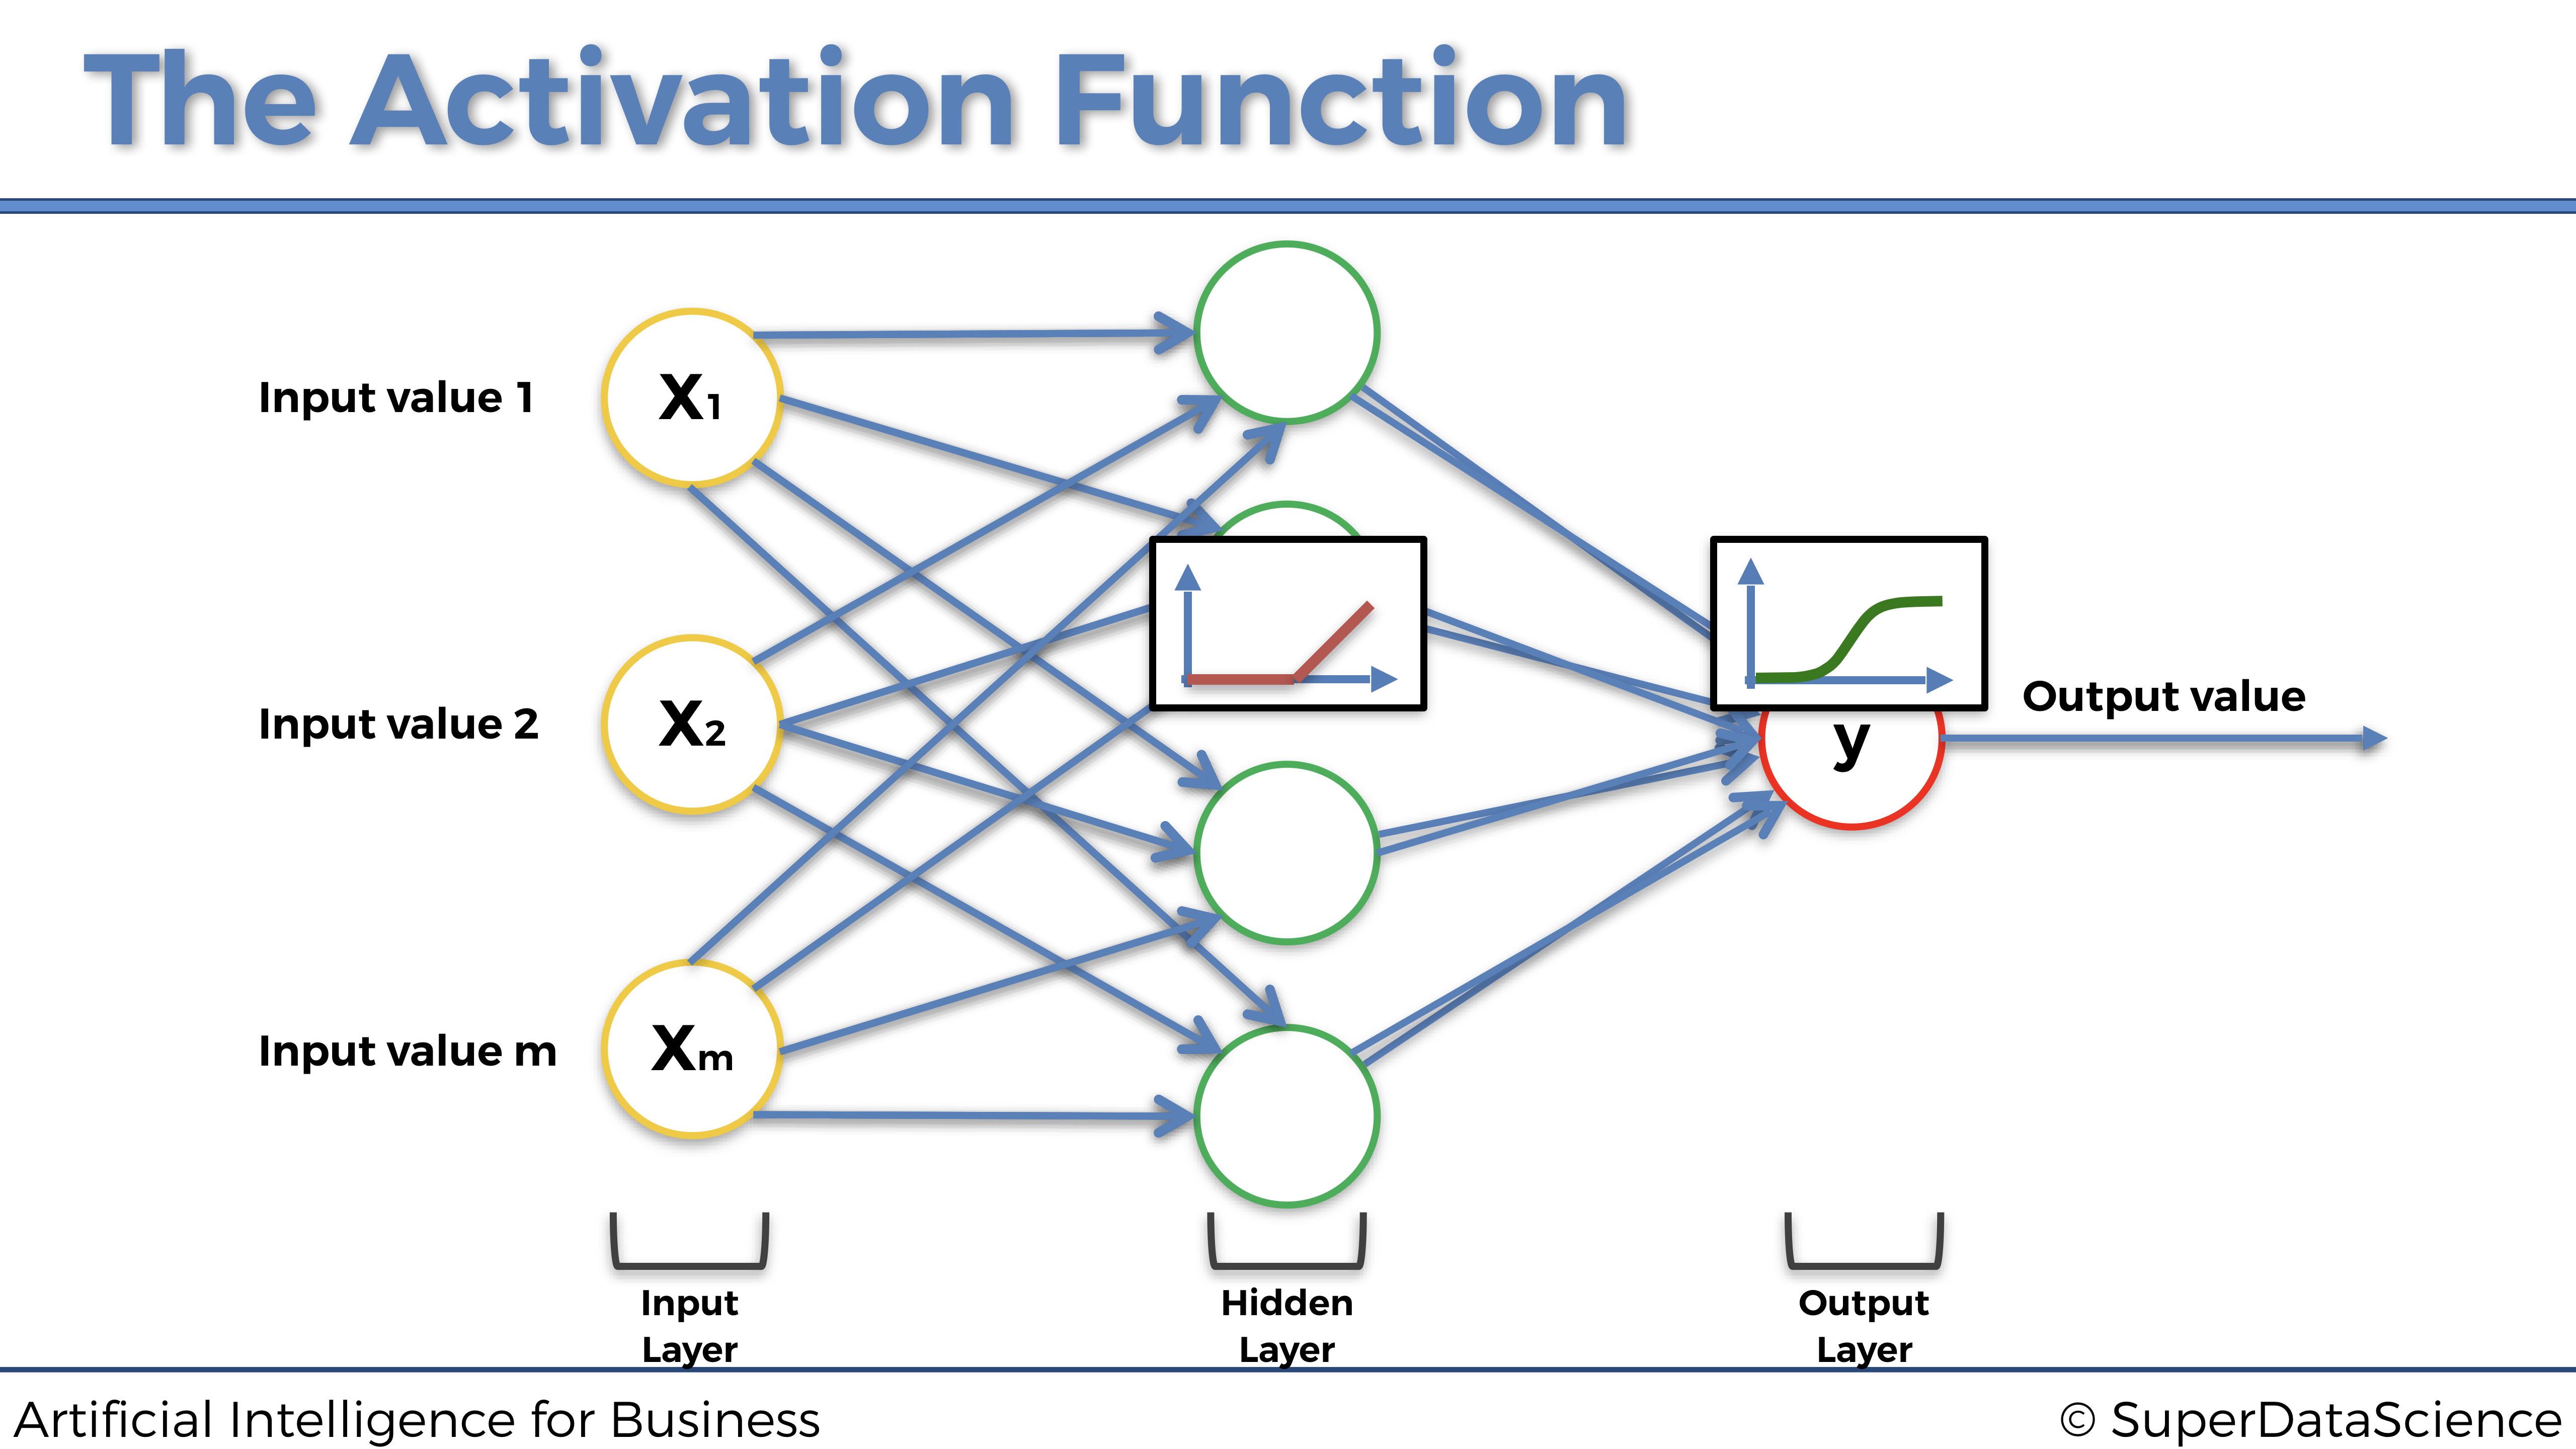
\includegraphics{Images/ANN_15.png}

Y, por último, ¿cómo elegir entre la función de activación del rectificador y la función de activación de la tangente hiperbólica en las capas ocultas? Pues es recomendable considerar usar la función de activación del rectificador cuando las entradas están normalizadas (escaladas entre 0 y 1), y la función de activación de Tangente hiperbólica cuando las entradas están estandarizadas (escaladas entre -1 y +1):

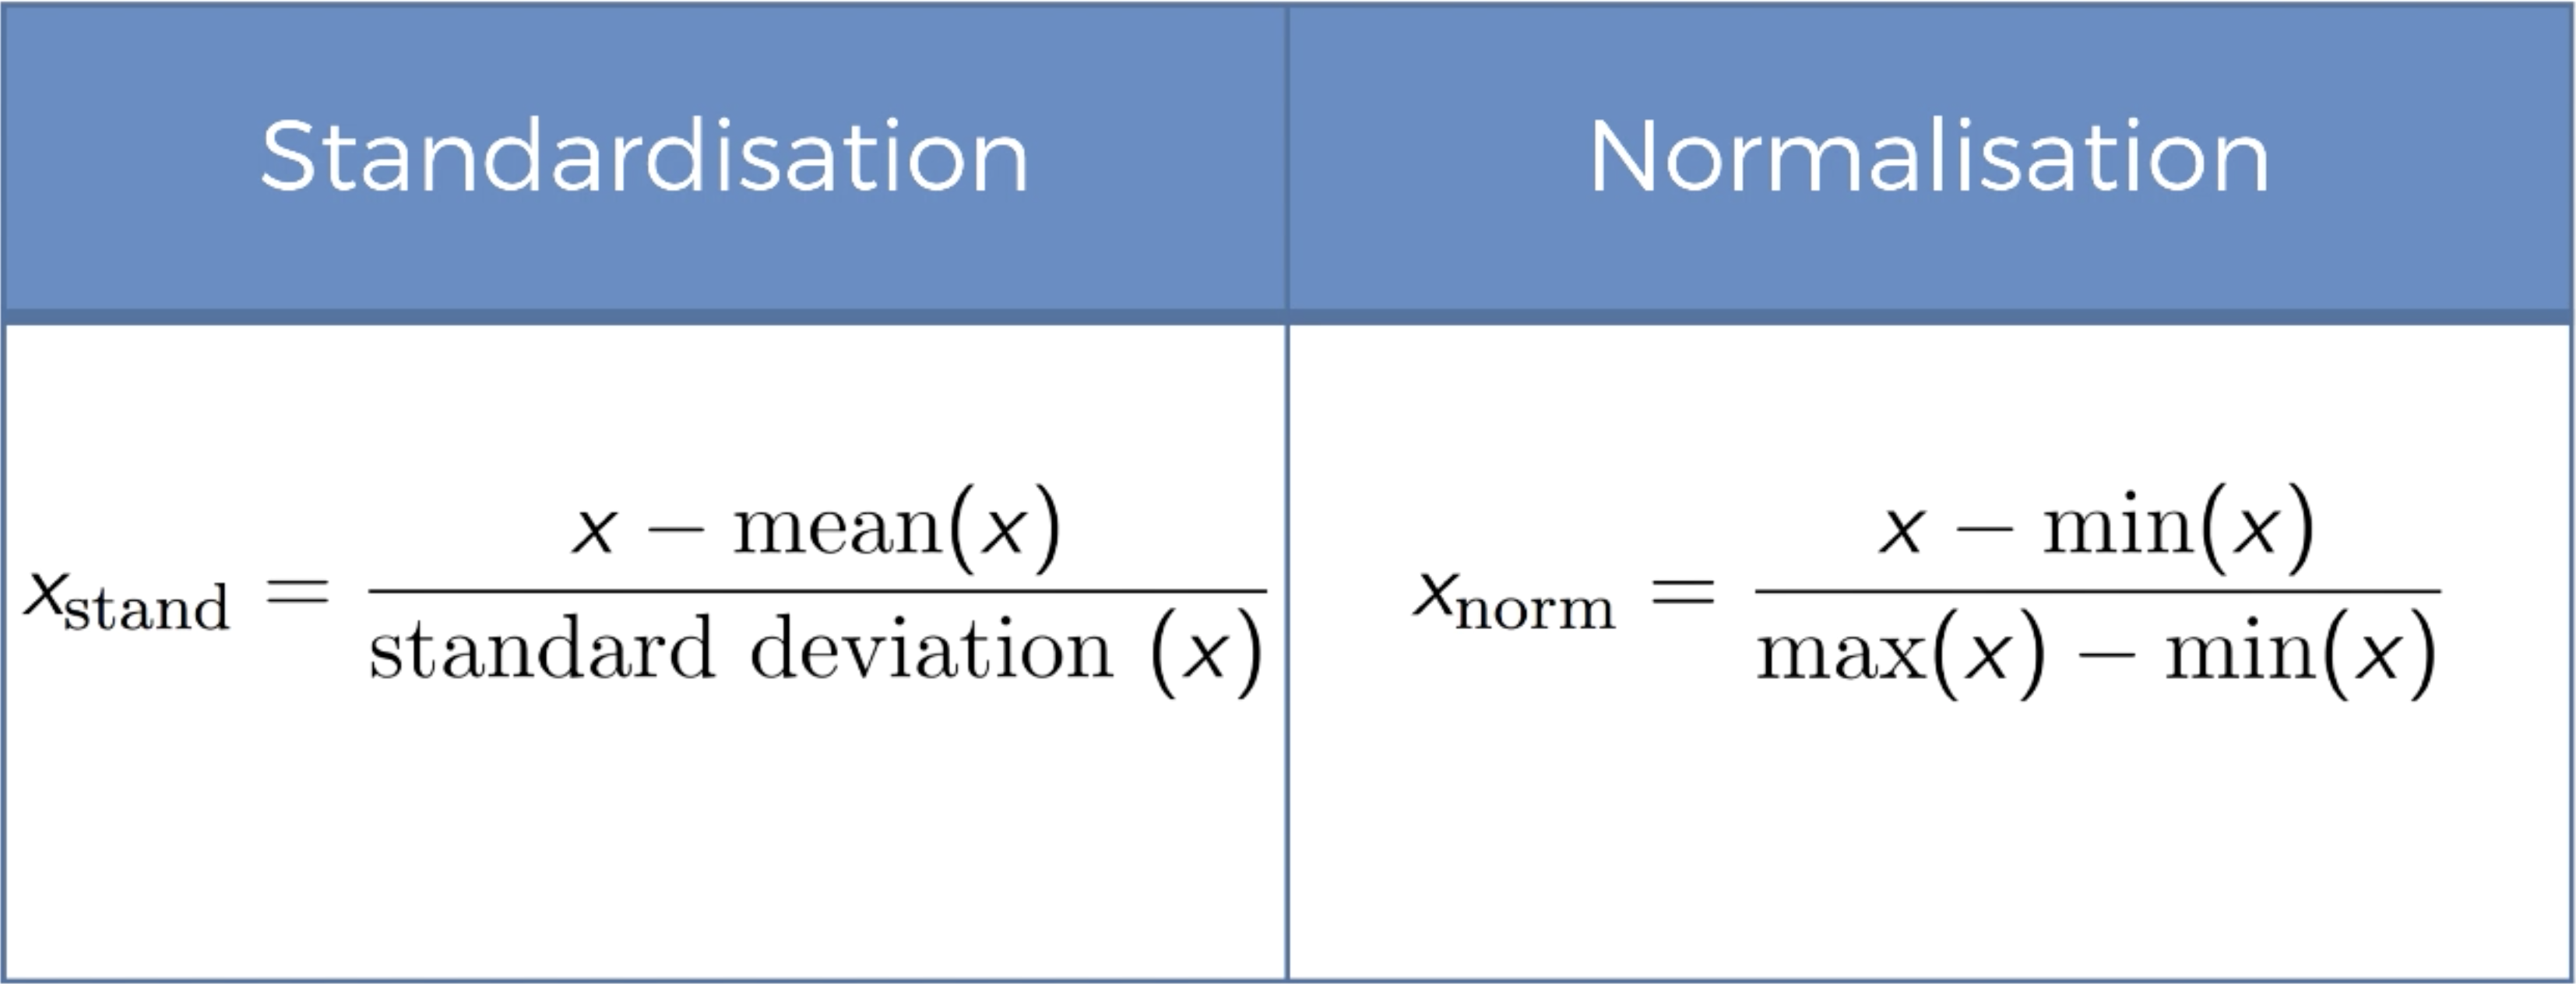
\includegraphics{Images/ANN_16.png}

Ahora pasemos a la siguiente sección para explicar cómo funcionan las redes neuronales.

\hypertarget{cuxf3mo-funcionan-las-redes-neuronales}{%
\subsection{¿Cómo funcionan las Redes Neuronales?}\label{cuxf3mo-funcionan-las-redes-neuronales}}

Para explicar esto, consideremos el problema de predecir los precios inmobiliarios. Tenemos algunas variables independientes que vamos a utilizar para predecir el precio de casas y apartamentos. Para simplificar, y para poder representar todo en un gráfico, digamos que nuestras variables independientes (nuestros predictores) son las siguientes:

\begin{itemize}
\tightlist
\item
  Área (pies cuadrados)
\item
  Número de habitaciones
\item
  Distancia a la ciudad (Millas)
\item
  Edad
\end{itemize}

Entonces, nuestra variable dependiente es, por supuesto, el precio del apartamento para predecir.

A cada una de las variables independientes se le atribuye un peso, de tal manera que cuanto mayor sea el peso, mayor será el efecto que tendrá la variable independiente en la variable dependiente, es decir, el predictor más fuerte será de la variable dependiente. Por lo tanto, tan pronto como nuevas entradas ingresen a la red neuronal, las señales se propagarán hacia adelante desde cada una de las entradas, llegando a la neuronas de la capa oculta. Luego, dentro de cada neurona de la capa oculta, se aplicará la función de activación, de modo que cuanto menor sea el peso de la entrada, la función de activación más bloqueará la señal procedente de esa entrada y cuanto mayor será el peso de esa entrada, la función de activación más permitirá que pase la señal a través de ella. Y finalmente, todas las señales procedentes de las neuronas ocultas, más o menos bloqueadas por las funciones de activación resppectivas, se propagan hacia la capa de salida, para devolver el resultado final, es decir, la predicción del precio.

Representemos esto en el siguiente gráfico:

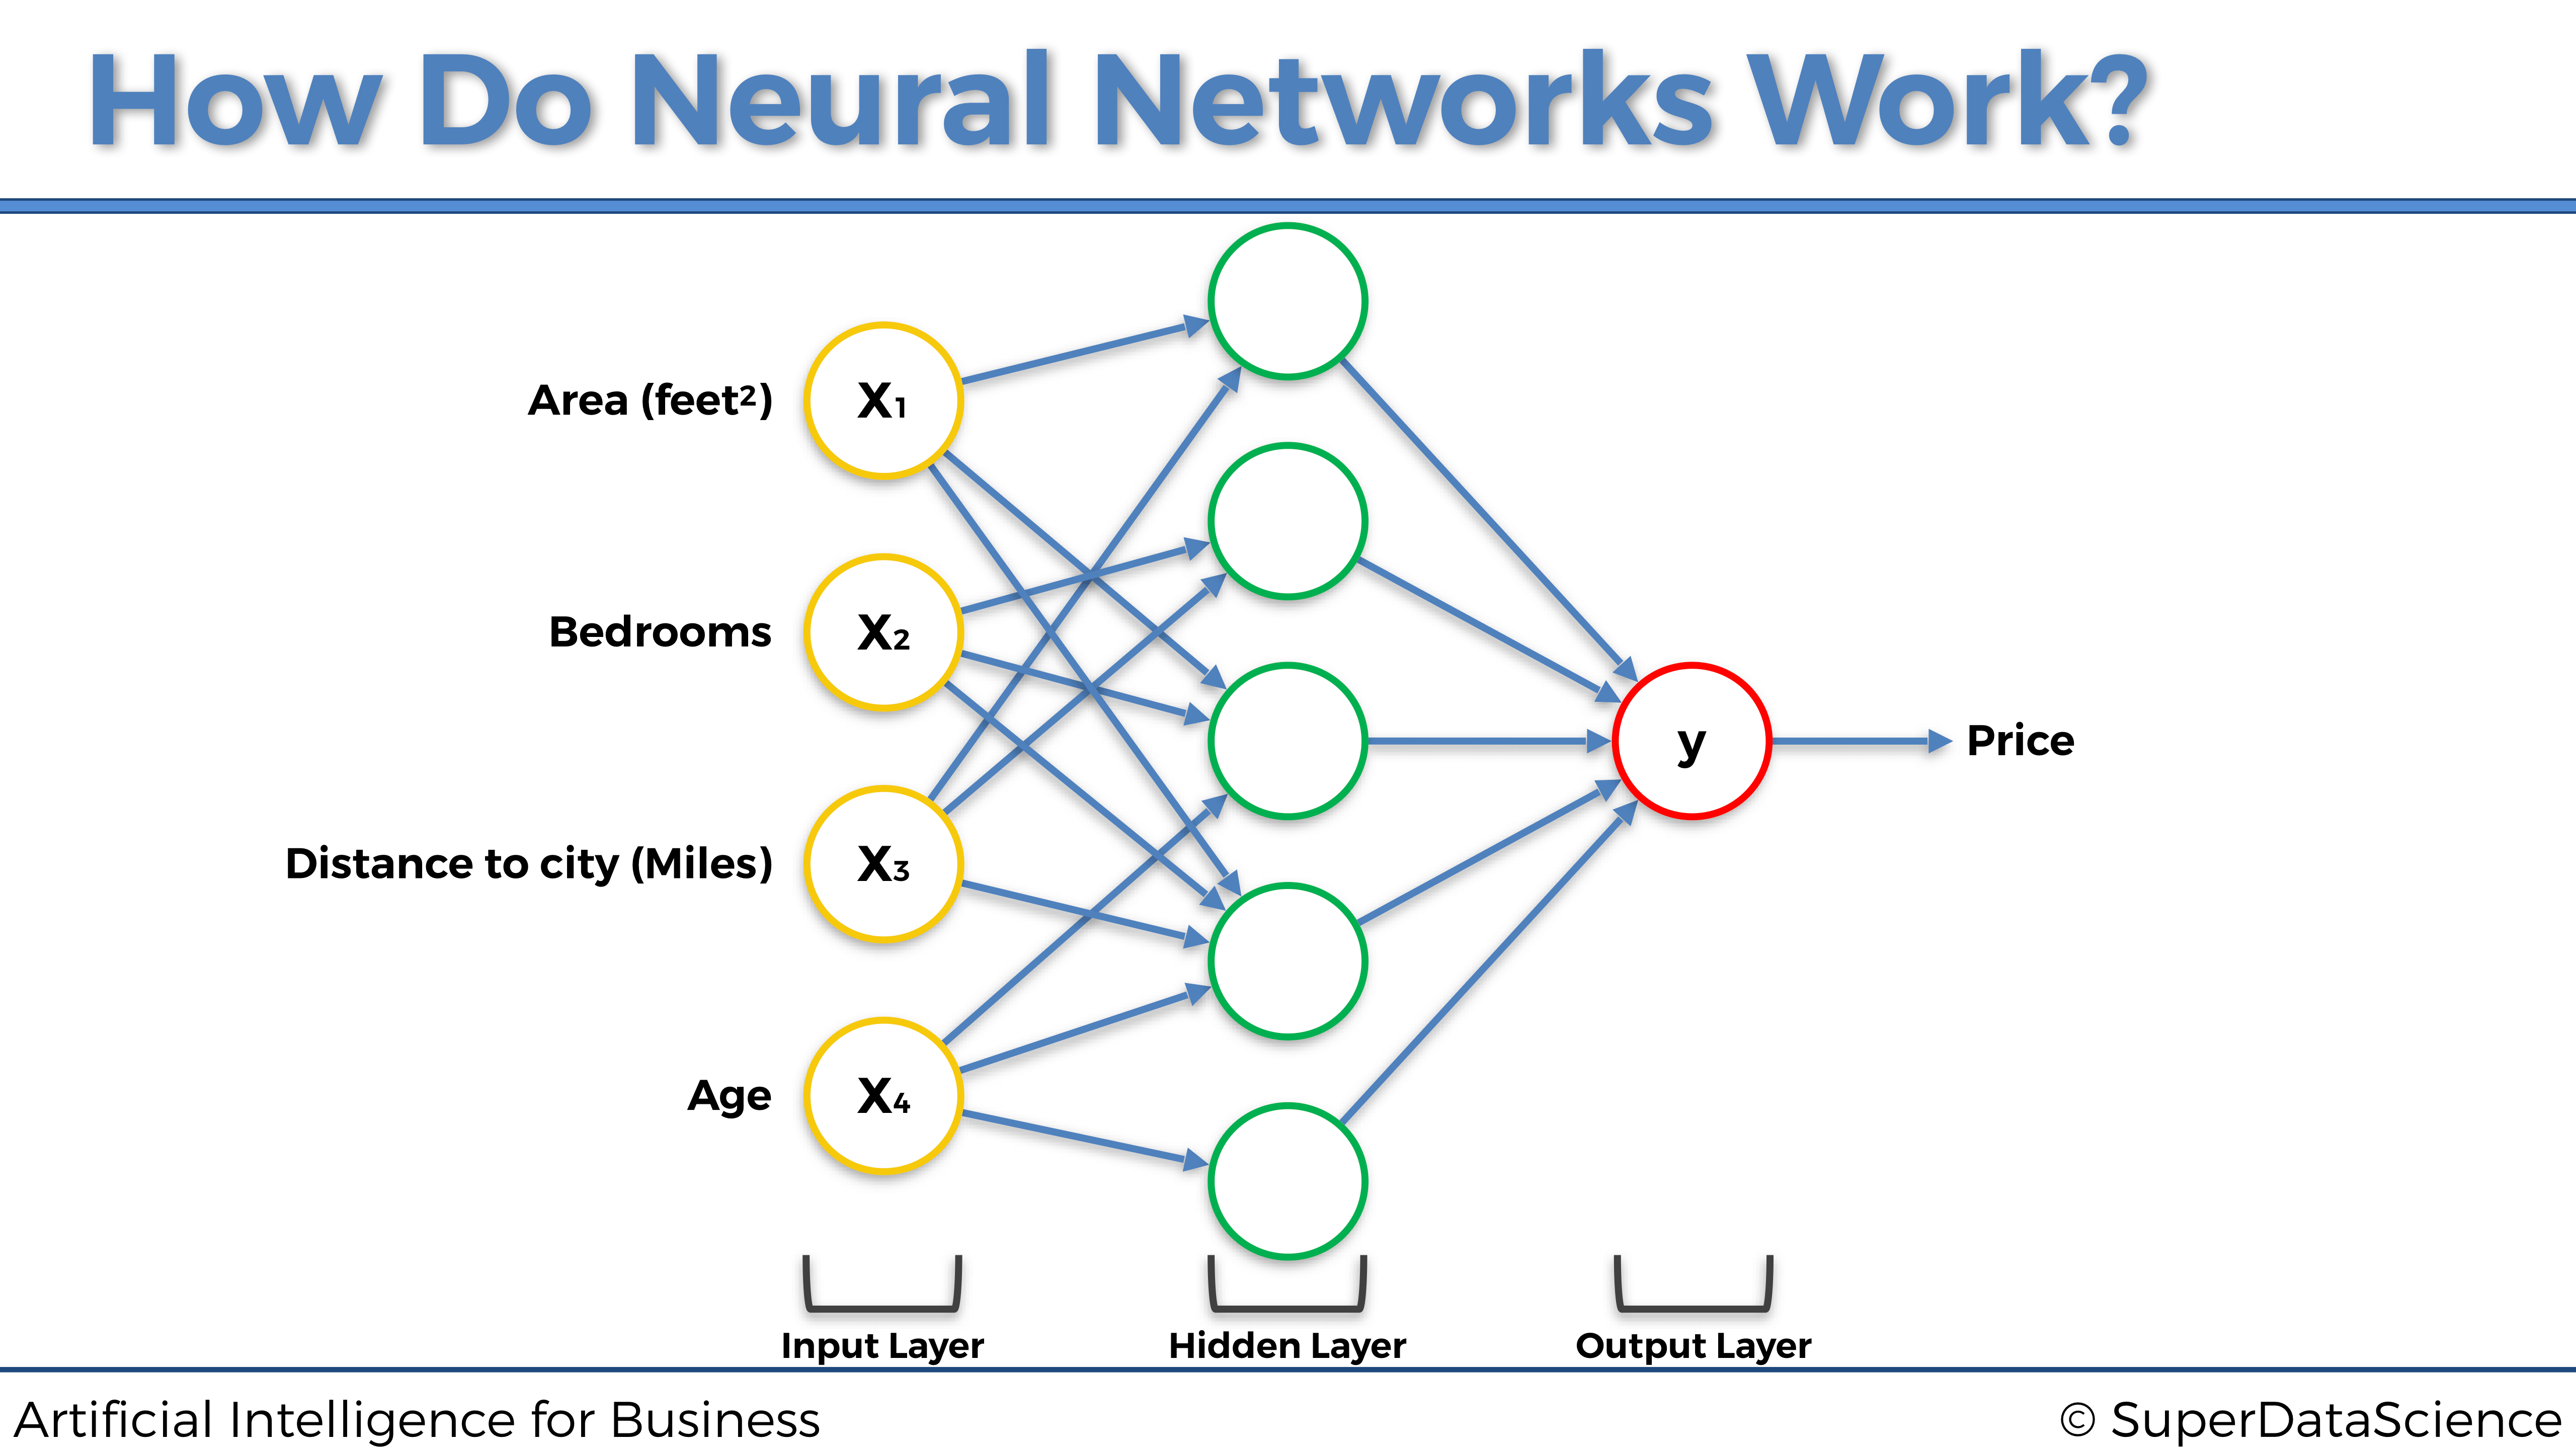
\includegraphics{Images/ANN_17.png}

\hypertarget{cuxf3mo-aprenden-las-redes-neuronales}{%
\subsection{¿Cómo aprenden las Redes Neuronales?}\label{cuxf3mo-aprenden-las-redes-neuronales}}

En pocas palabras, las redes neuronales aprenden actualizando, durante muchas iteraciones llamadas \texttt{epochs}, los pesos de todas las entradas y neuronas ocultas (cuando tienen varias capas ocultas), hacia siempre el mismo objetivo: el de reducir el error de pérdida entre las predicciones y los valores reales.

De hecho, para que las Redes Neurales aprendan, necesitamos los valores reales, que también se denominan objetivos. En nuestro ejemplo anterior sobre la fijación de precios inmobiliarios, los valores reales son los precios reales de las casas y apartamentos en ventas. Estos precios reales dependen de las variables independientes enumeradas anteriormente (área, número de habitaciones, distancia a la ciudad y edad), y la red neuronal aprenderá a hacer mejores predicciones de estos precios, ejecutando el siguiente proceso:

\begin{itemize}
\tightlist
\item
  La red neuronal primero propaga las señales procedentes de las variables independientes de entrada \(x_1\), \(x_2\), \(x_3\) y \(x_4\).
\item
  Luego obtiene el precio predicho \(\hat{y}\) en la capa de salida.\\
\item
  Luego calcula el error de pérdida \(C\) entre el precio predicho \(\hat{y}\) (predicción) y el precio real \(y\) (objetivo):
\end{itemize}

\[C = \frac{1}{2} (\hat{y} - y)^2\]

\begin{itemize}
\tightlist
\item
  Luego, este error de pérdida se propaga hacia atrás dentro de la red neuronal, de derecha a izquierda en nuestra representación.\\
\item
  Luego, en cada una de las neuronas, la red neuronal ejecuta una técnica llamada Gradiente Descendente (que discutiremos en la siguiente sección), para actualizar los pesos en la dirección de reducción de pérdidas, es decir, en nuevos pesos que reducen el error de pérdida \(C\).\\
\item
  Luego, todo este proceso se repite muchas veces, con cada vez nuevas entradas y nuevos objetivos, hasta que obtenemos el rendimiento deseado (detención temprana o \emph{early stopping}) o la última iteración (número de iteraciones elegidas en la implementación).
\end{itemize}

Representemos las dos fases principales, Propagación hacia adelante y Propagación hacia atrás, de todo este proceso en los dos gráficos siguientes:

\hypertarget{propagaciuxf3n-hacia-adelante-and-propagaciuxf3n-hacia-atruxe1s}{%
\subsection{Propagación hacia adelante and propagación hacia atrás}\label{propagaciuxf3n-hacia-adelante-and-propagaciuxf3n-hacia-atruxe1s}}

\textbf{Fase 1: Propagación hacia adelante:}

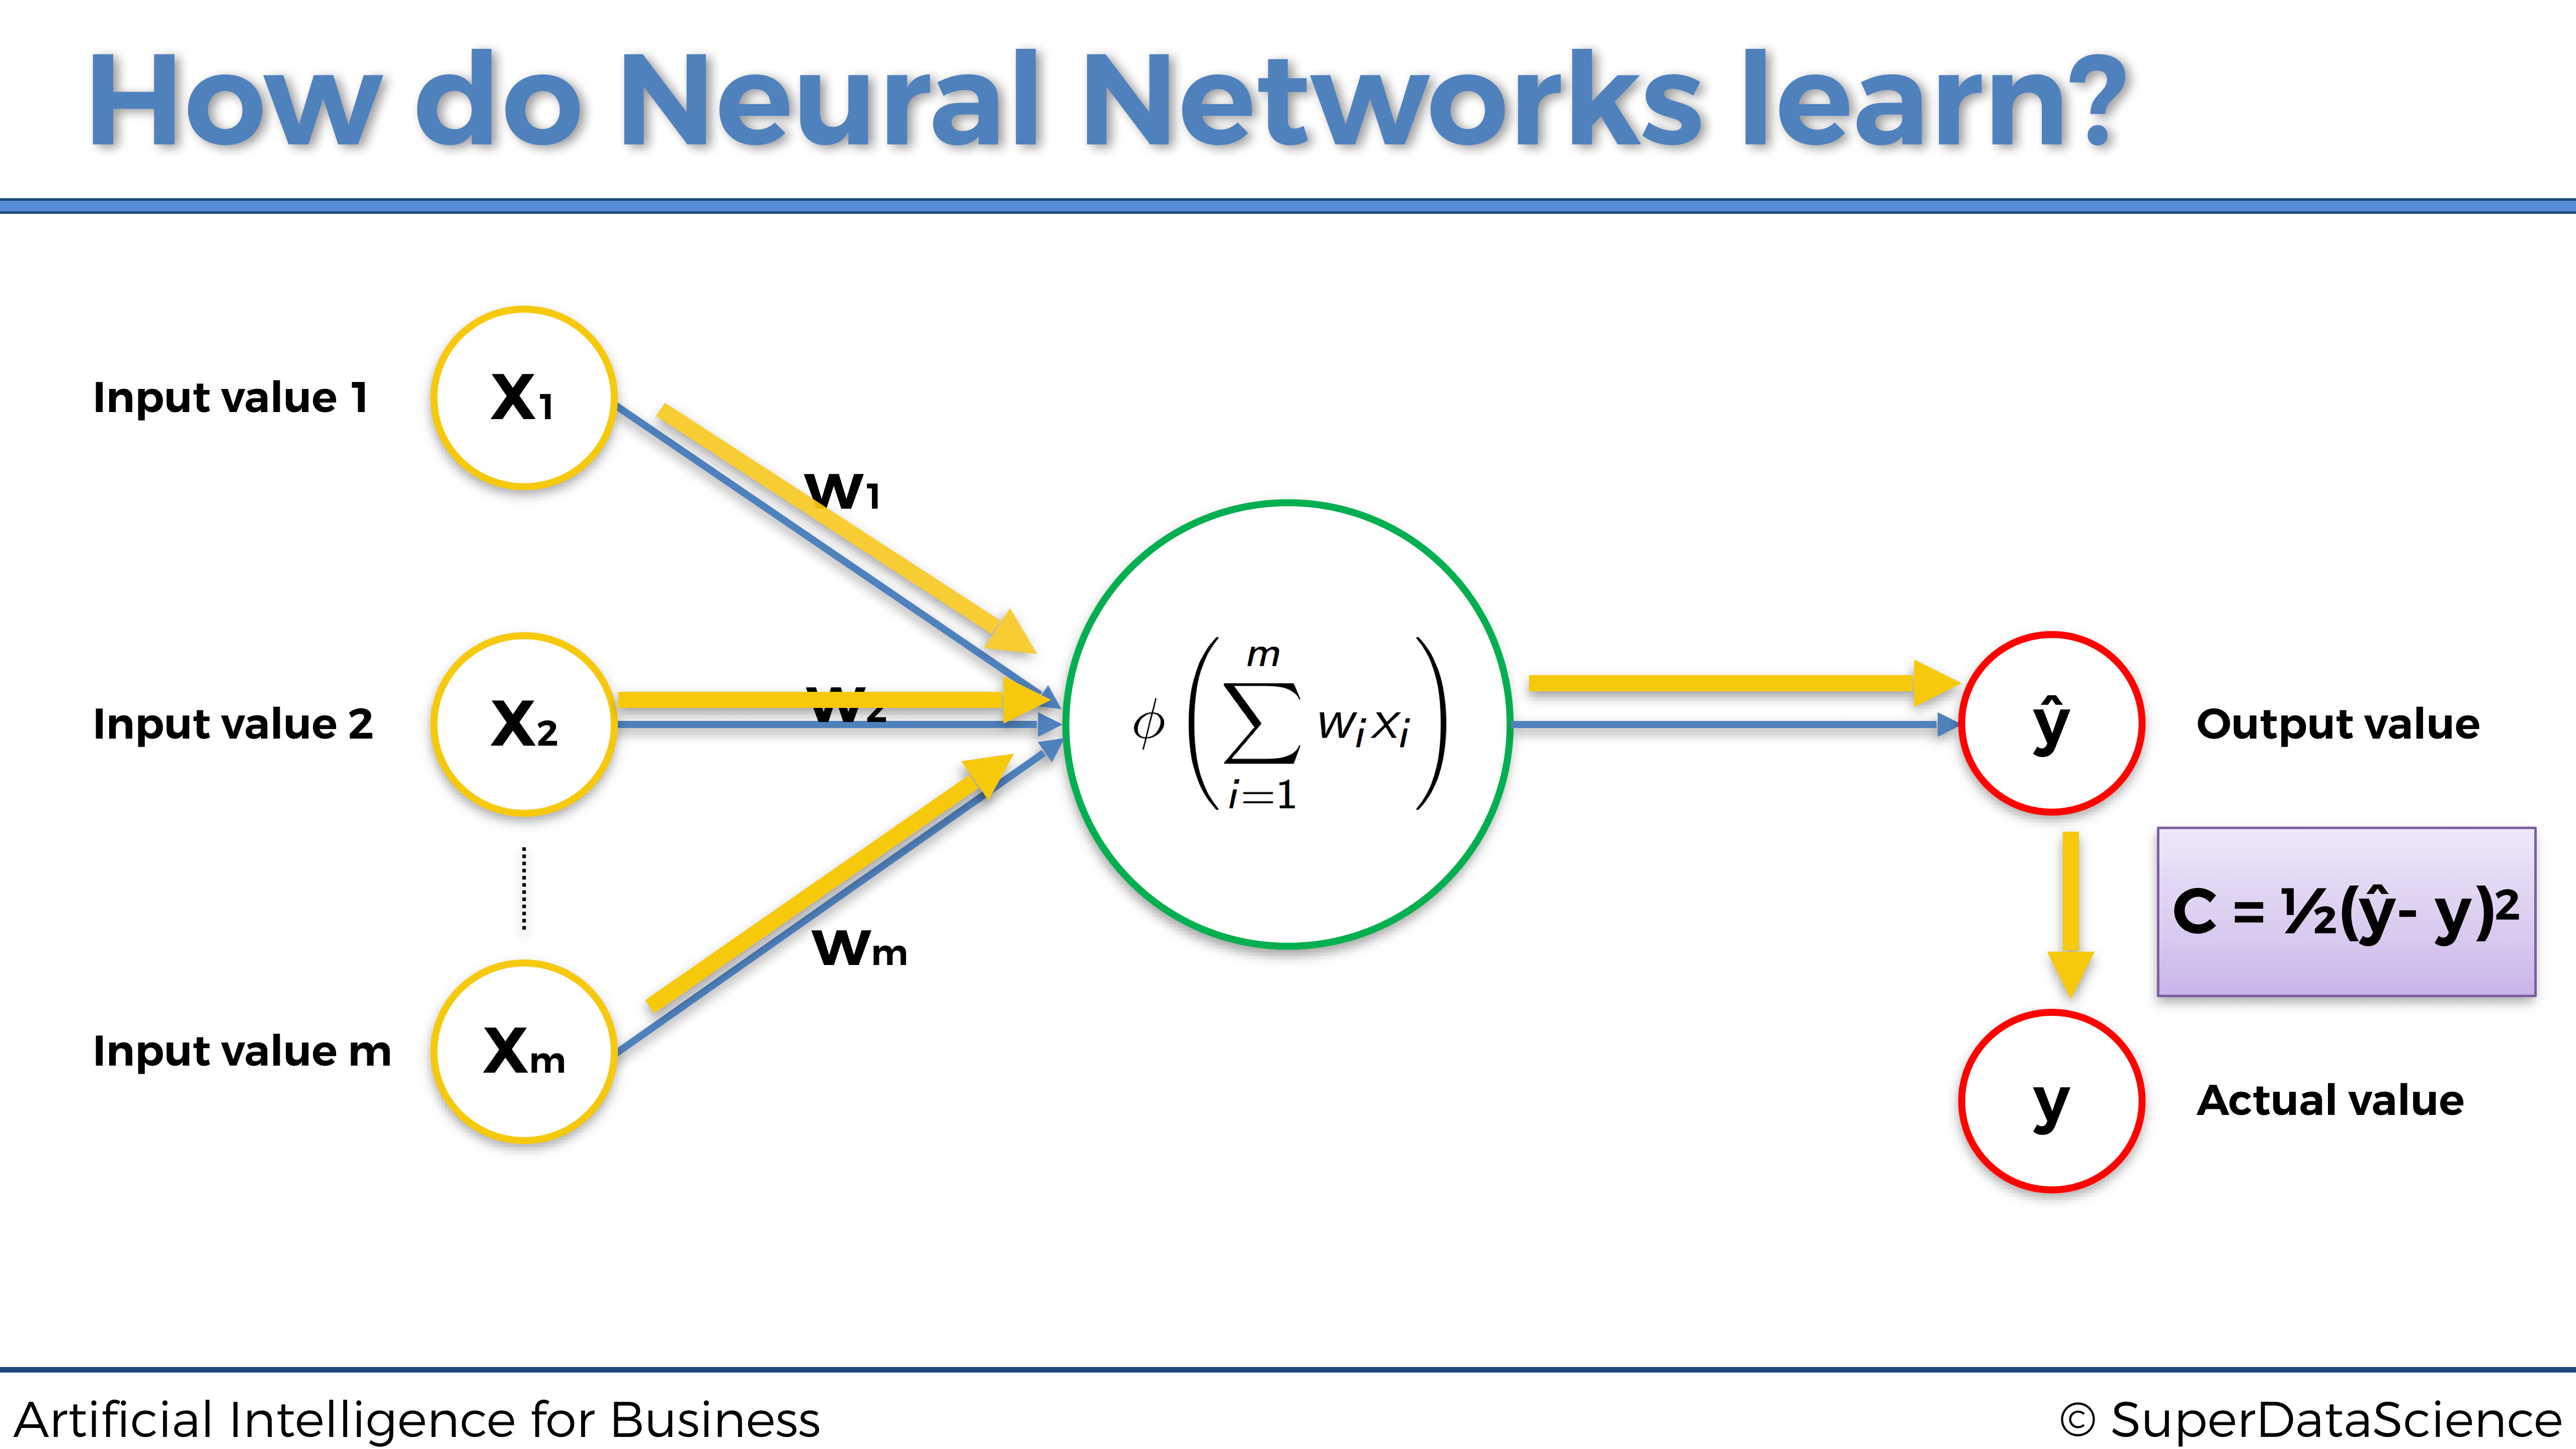
\includegraphics{Images/ANN_18.png}

\textbf{Fase 2: Propagación hacia atrás:}

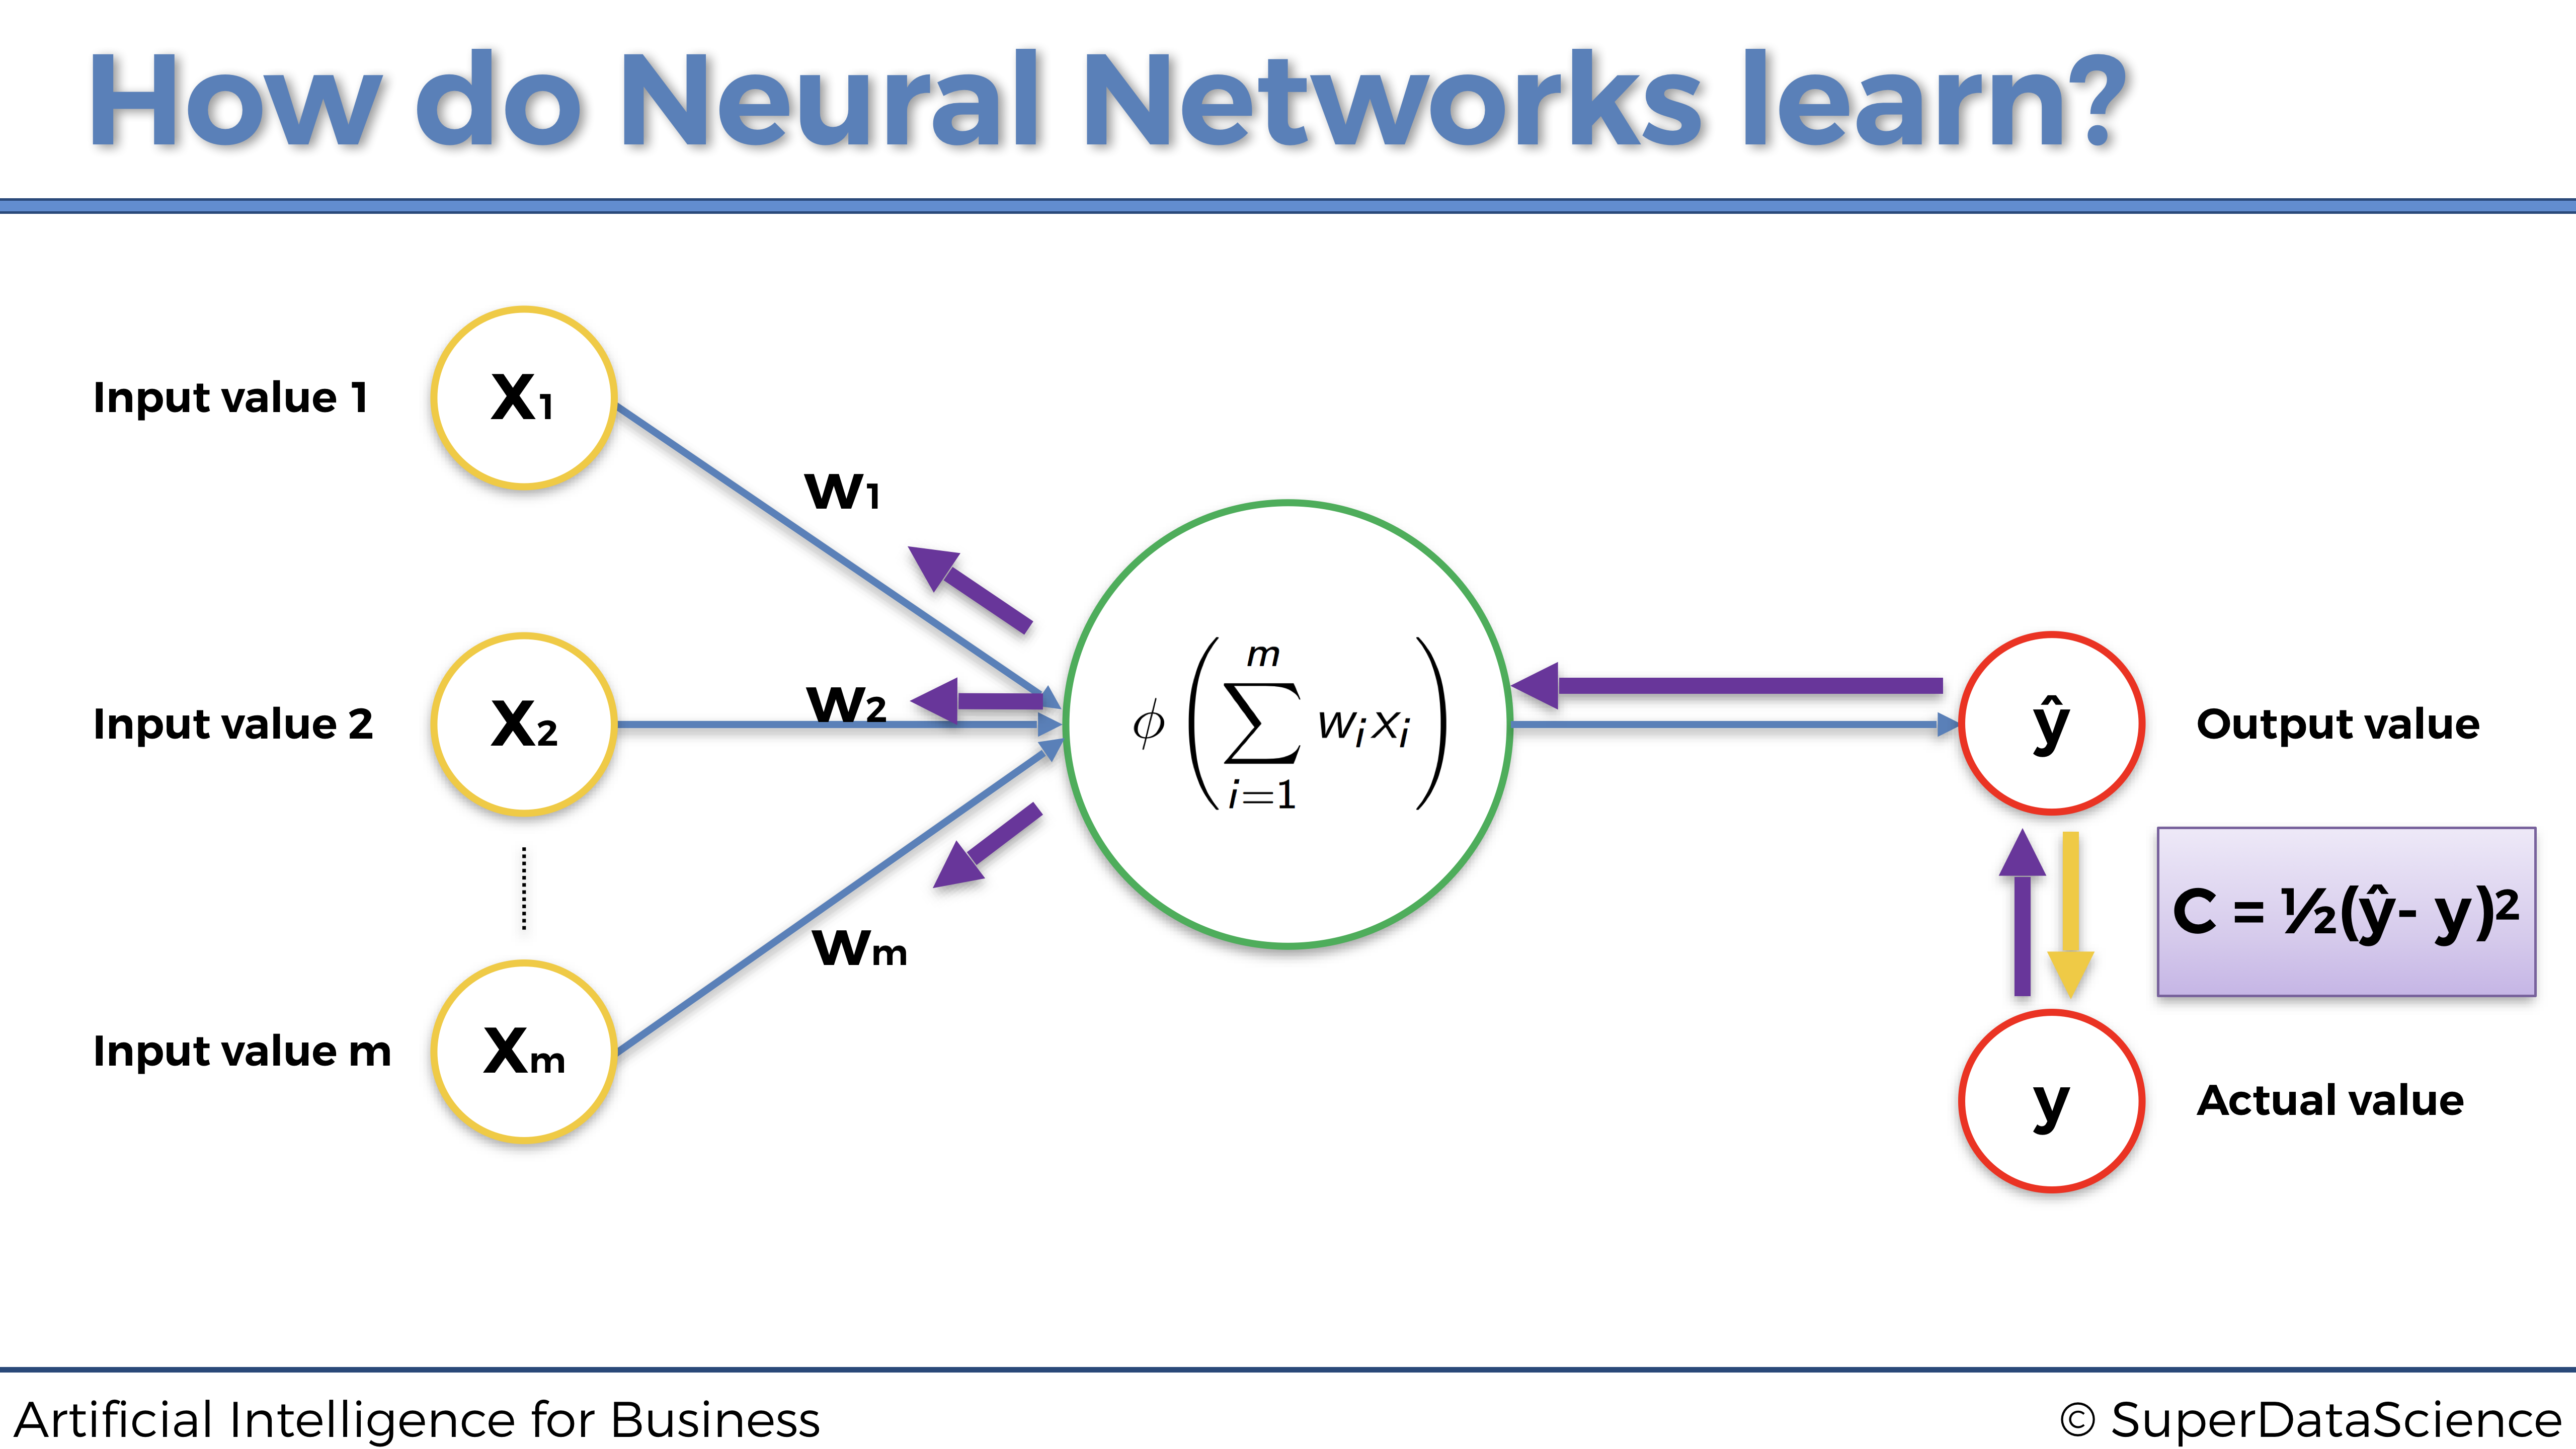
\includegraphics{Images/ANN_19.png}

\hypertarget{gradiente-descendente}{%
\subsection{Gradiente Descendente}\label{gradiente-descendente}}

\hypertarget{introducciuxf3n-al-gradiente-descendente}{%
\subsubsection{Introducción al Gradiente Descendente}\label{introducciuxf3n-al-gradiente-descendente}}

Cuando las personas hablan de Machine Learning o Deep Learning, hablan principalmente de los algoritmos que se utilizan. Pero las preguntas reales son, ¿por qué se considera que esos algoritmos son algoritmos de Aprendizaje automático o Aprendizaje profundo y otros no? ¿Cuál es la técnica subyacente que los diferencia?

La respuesta a la primera pregunta es bastante intuitiva: se considera que esos algoritmos aprenden sus parámetros por sí mismos. Esta propiedad no era muy común antes y la mayoría de los algoritmos fueron ajustados a mano por ingenieros para lograr una especificación / meta requerida.

Pero entonces apareció la idea de incorporar el Gradiente Descendente a los mismos y la mayoría de los algoritmos que no funcionaban antes, de repente tuvieron sentido y comenzaron a optimizarse.

Entonces, ¿es mágica la técnica del Gradiente Descendente? Bueno, para alguien lo podría ser, pero para nosotros es un algoritmo matemático que se utiliza para optimizar un modelo que tiene sus parámetros internos (pesos). O, para ser más técnicos, veamos qué dice Wikipedia al respecto:

\begin{quote}
``El Gradiente Descendente es un algoritmo de optimización iterativa de primer orden para encontrar el mínimo de una función''.
\end{quote}

Esa es una definición correcta pero con poco contenido, y para alguien que recién está comenzando, ¡encima es aterradora! Vamos a desglosarlo:

\begin{itemize}
\tightlist
\item
  \textbf{Algoritmo}: en pocas palabras, es un plan sobre cómo resolver un problema. El ejemplo cotidiano de un algoritmo sería una receta de cocina.
\item
  \textbf{Iterativo}: esto significa que utiliza algún tipo de bucle (para programadores, bucles \texttt{for} o \texttt{while}) para realizar pasos. Cada paso usa valores calculados previamente como entrada para el paso actual. Ahora, surge una pregunta: ``¿Cuál es nuestro valor inicial?''. Responderemos sobre esto un poco más adelante a través de ejemplos.
\item
  \textbf{Optimización}: intenta encontrar las mejores soluciones de acuerdo con algunos criterios que conducen a varias soluciones alternativas, pero solo una se considera la mejor.
\item
  \textbf{De primer orden} ElGradiente Descendente está utilizando la primera derivada de una función de criterio elegida (coste, pérdida) para encontrar cuál es una mejor solución para el problema dado.
\end{itemize}

Por lo tanto, cuando lo ponemos todo junto en palabras inteligibles, obtenemos la siguiente definición:

\begin{quote}
El Gradiente Descendente es un plan sobre cómo encontrar la mejor solución para un problema donde más de una solución es aceptable. Utiliza un objetivo para determinar qué tan lejos estamos de encontrar la mejor solución.
\end{quote}

Hasta este punto, tenemos todo aclarado, excepto la función de costes.

El coste es el indicador que seguimos durante el proceso de optimización. En base a ese indicador, podemos decir qué tan lejos estamos del óptimo de una función. Un buen ejemplo del costo es el error cuadrático medio, que hemos visto anteriormente en este libro:

\[\textrm{MSE} = \frac{1}{n} \sum_{i=1}^n (y_i - \hat{y}_i)\]

donde:

\[
\begin{cases}
        \textrm{$\hat{y}_i$ es la predicción del modelo} \\
        \textrm{$y_i$ es el objetivo (el valor actual)} \\
        \textrm{$n$ es el número de muestras del data set}
    \end{cases}
\]

Cada algoritmo que utiliza el Gradiente Descendente como técnica de optimización tiene parámetros (pesos) que cambian durante el proceso de optimización. Cuando decimos que estamos buscando el mínimo de la función de pérdida, en realidad queremos decir que estamos buscando los valores de los pesos para los cuales la pérdida tiene el valor más bajo posible.

En consecuencia, para responder a nuestra segunda pregunta desde el principio, el punto en común que tienen todos los algoritmos de Aprendizaje automático desde la regresión lineal a las redes neuronales más complicadas es, de hecho, el Gradiente Descendente.

\hypertarget{idea-del-gradiente-descendente}{%
\subsubsection{Idea del Gradiente Descendente}\label{idea-del-gradiente-descendente}}

Como hemos visto, el Gradiente Descendente es una técnica de optimización que nos ayuda a encontrar el mínimo de una función de costo. Ahora visualicémoslo de la manera más intuitiva, como la siguiente bola en un bol (junro con un poco de espray matemático encima):

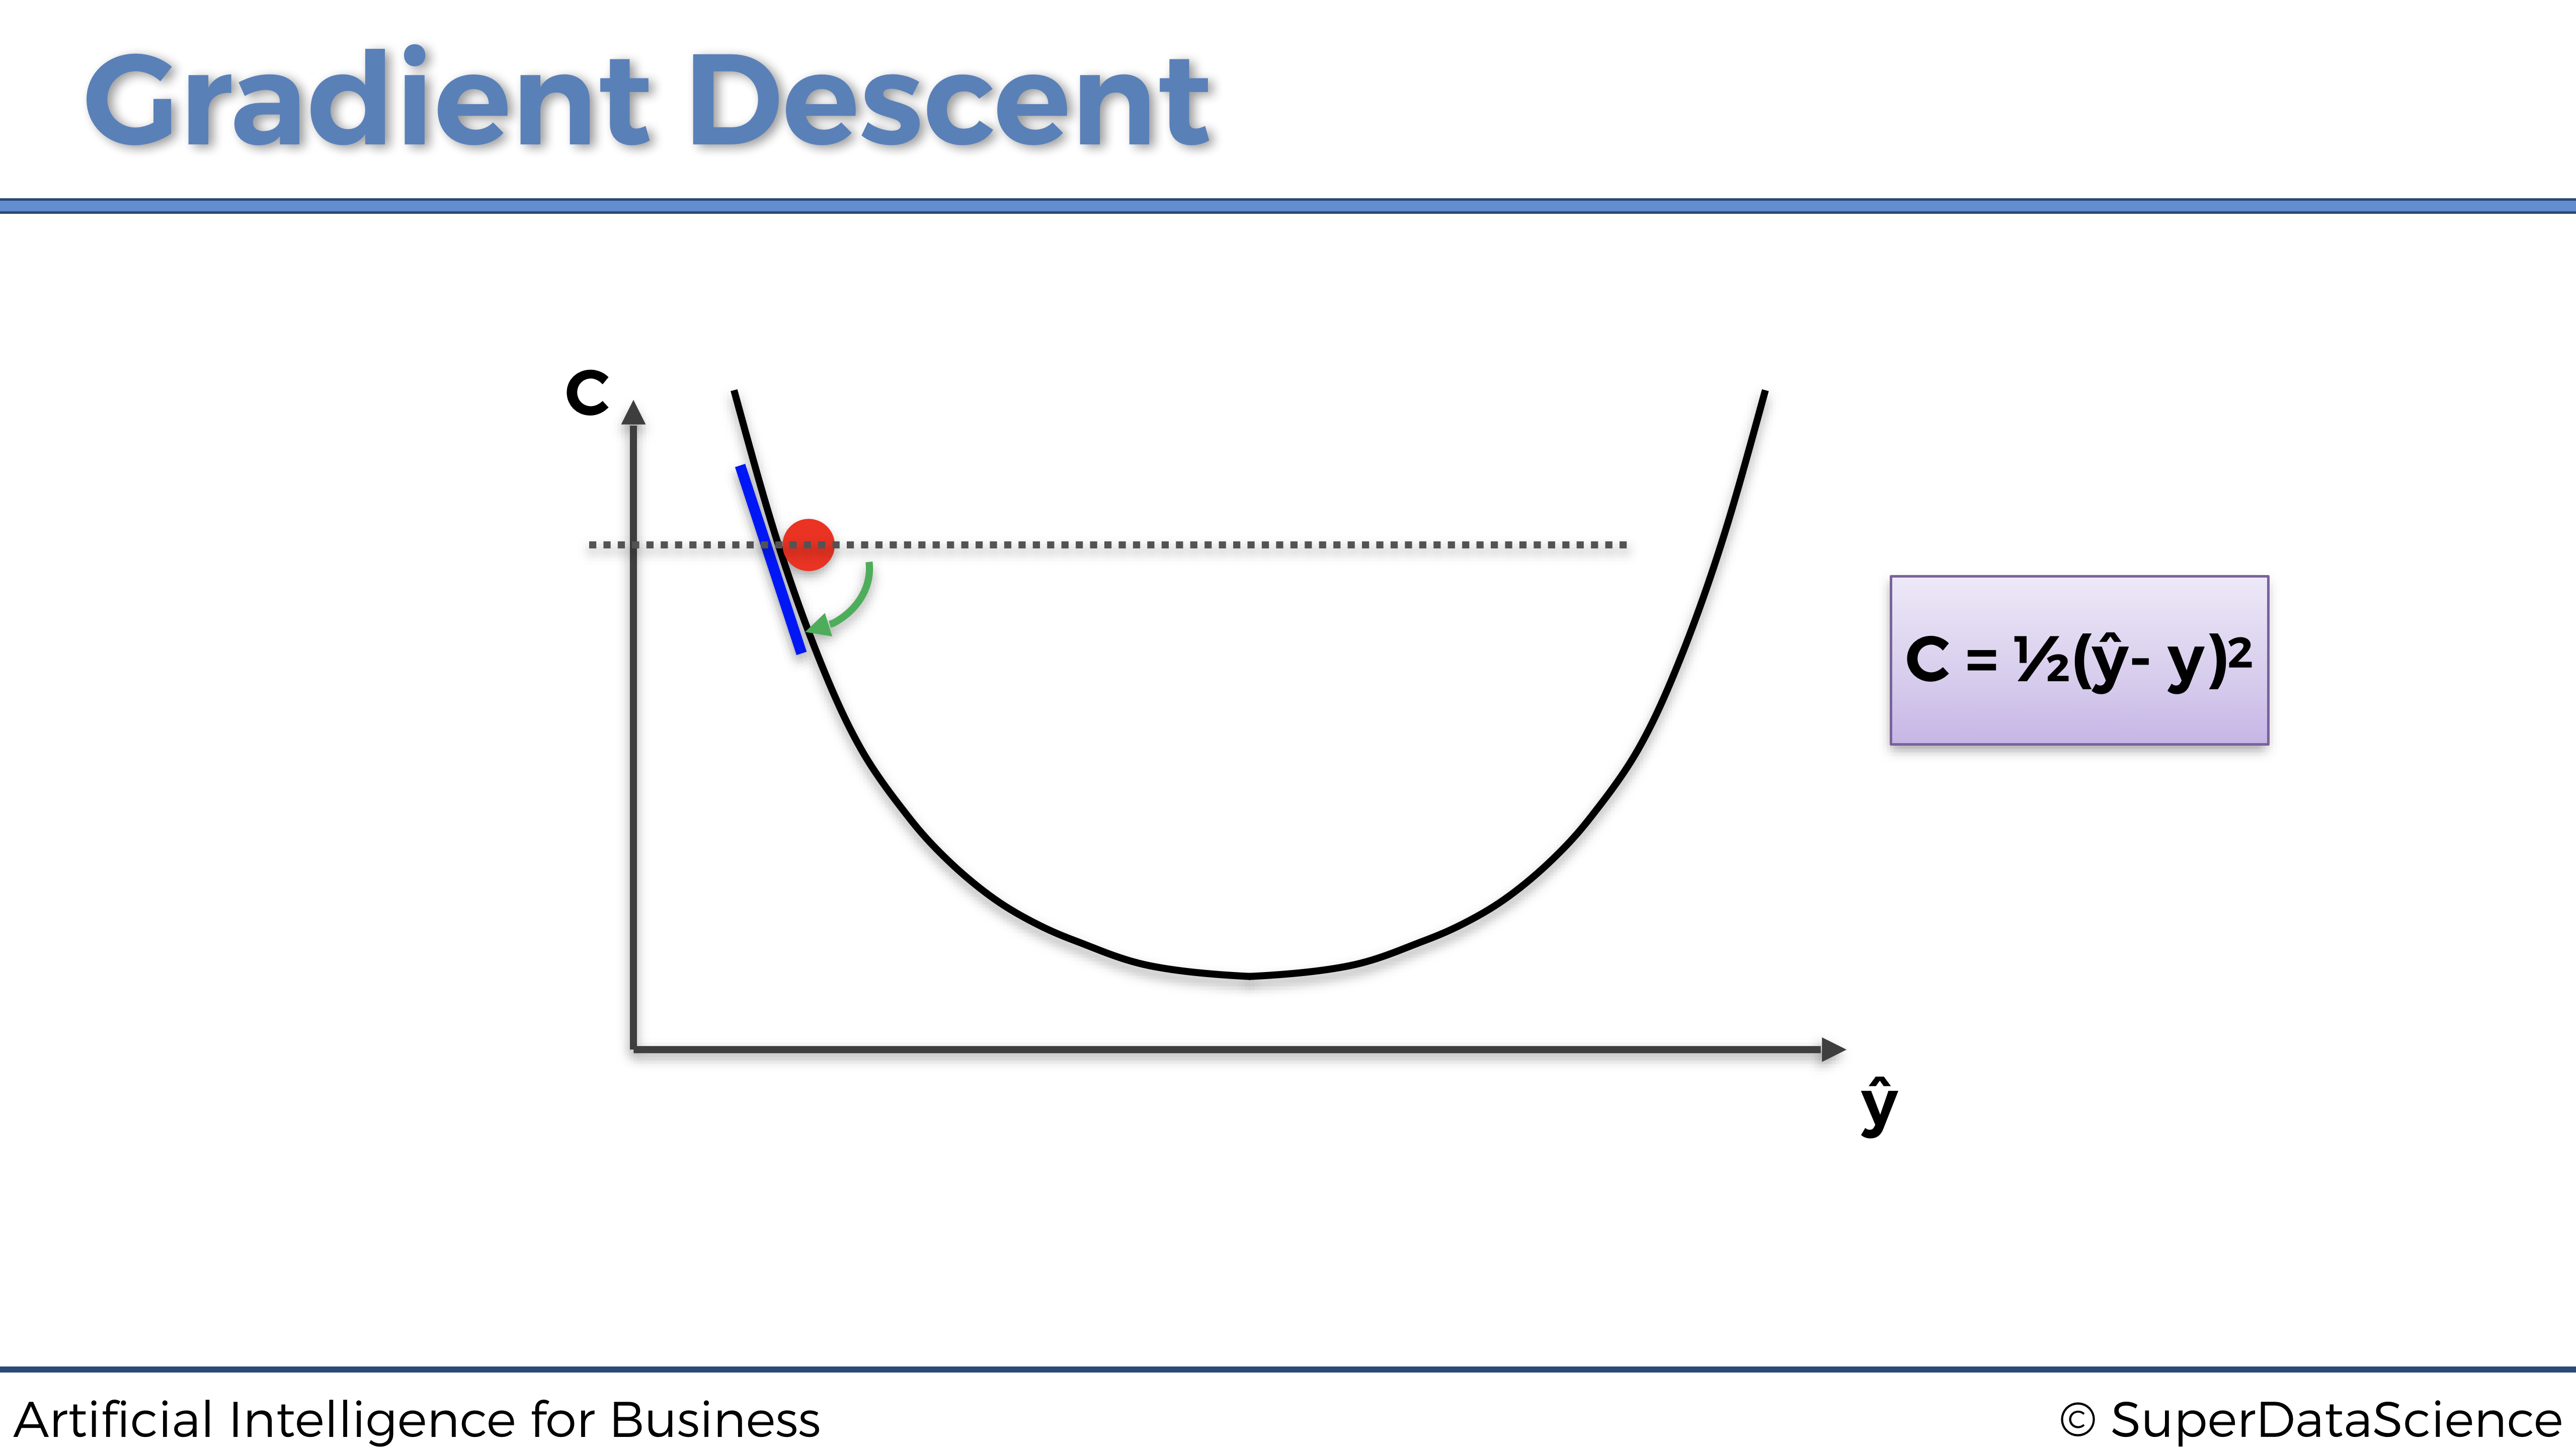
\includegraphics{Images/ANN_20.png}

Imagina que esta es una sección transversal de un bol, dentro del cual dejamos caer una pequeña bola roja y dejamos que llegue al fondo del mismo Después de un tiempo dejará de rodar, ya que ha encontrado el punto ideal para ello, en el fondo del tazón.

Puedes pensar en el Gradiente Descendente de la misma manera. Comienza en algún lugar del bol (valores iniciales de los parámetros) e intenta encontrar el fondo del mismo, o en otras palabras, el mínimo de una función de coste.

Veamos el ejemplo que se muestra en la imagen de arriba. Los valores iniciales de los parámetros han establecido nuestra bola en la posición que se muestra. En base a eso obtenemos algunas predicciones, que comparamos con nuestros valores objetivo. La diferencia entre estos dos conjuntos será nuestra pérdida para el conjunto actual de parámetros.

Luego calculamos la primera derivada de la función de coste, con respecto a los parámetros. De aquí proviene el nombre \textbf{Gradient}. Aquí, esta primera derivada nos da la pendiente de la tangente a la curva donde está la bola. Si la pendiente es negativa, como en la imagen de arriba, damos el siguiente paso hacia el lado derecho. Si la pendiente es positiva, damos el siguiente paso hacia el lado izquierdo.

El nombre \textbf{Descendente} proviene del hecho de que siempre damos el siguiente paso que apunta hacia abajo, como se representa en el siguiente gráfico:

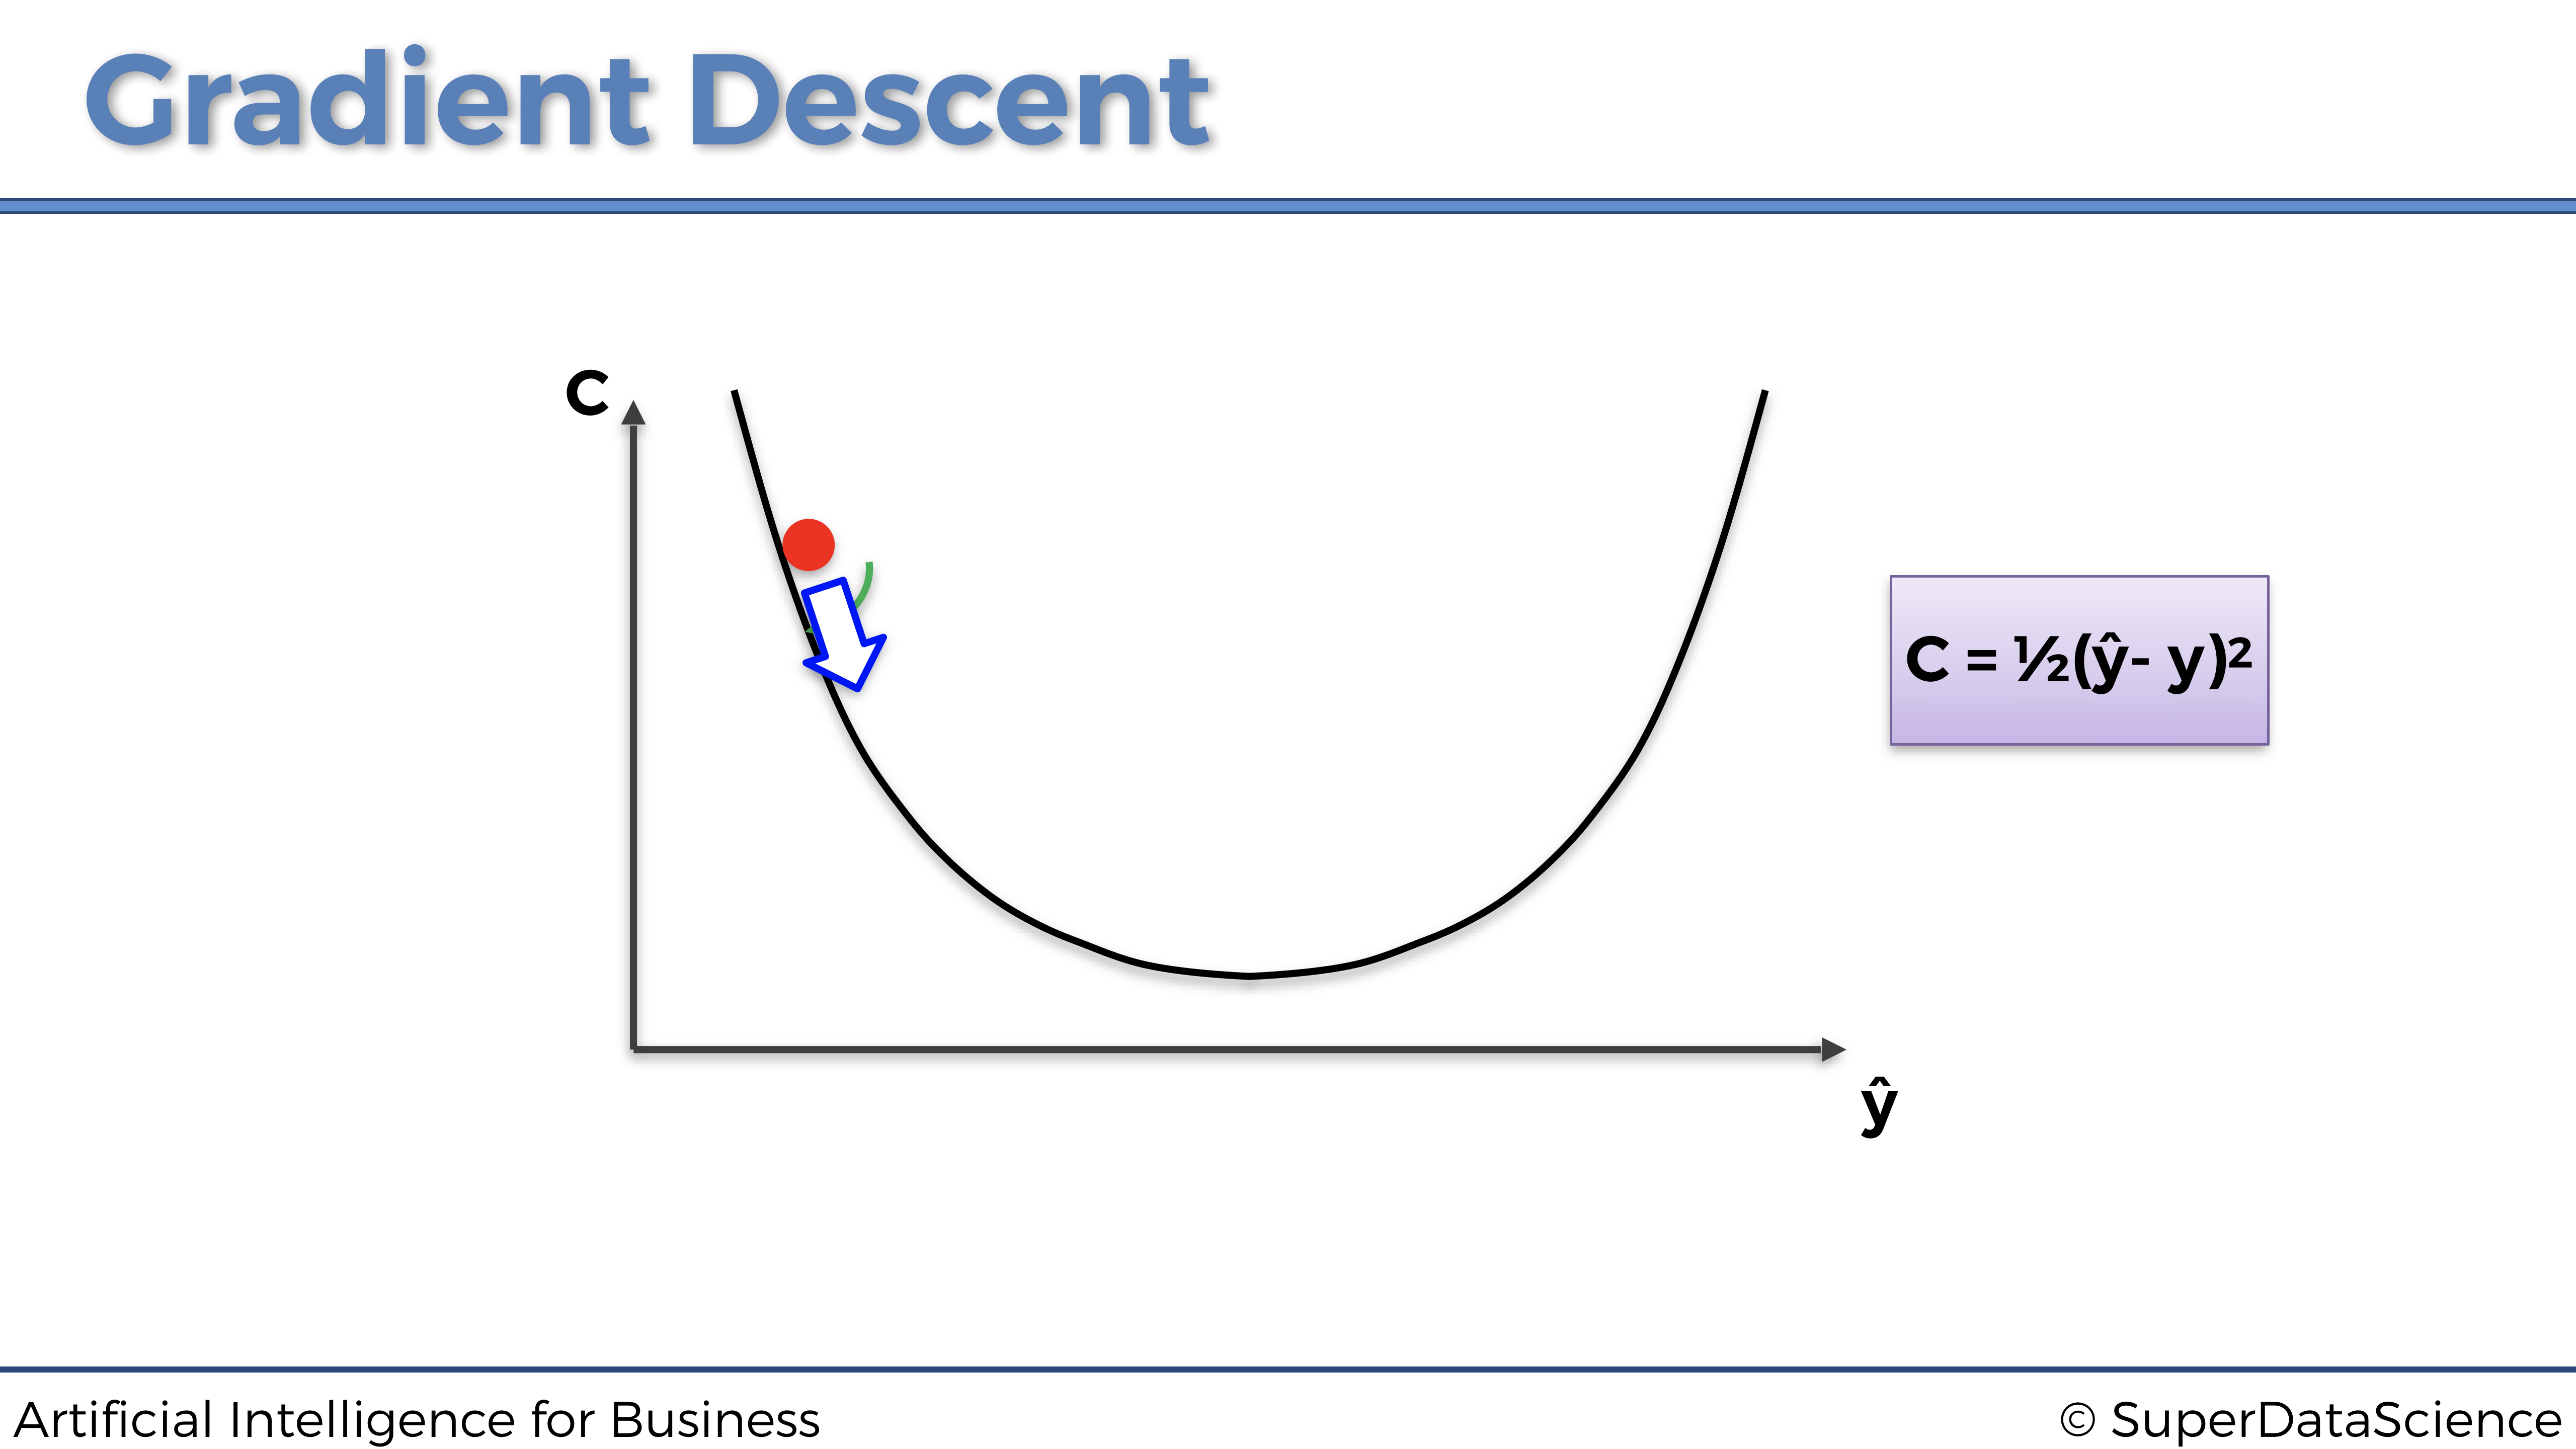
\includegraphics{Images/ANN_21.png}

Ahora, en esta posición, nuestra pelota tiene una pendiente positiva, por lo que debemos dar el siguiente paso hacia la izquierda.

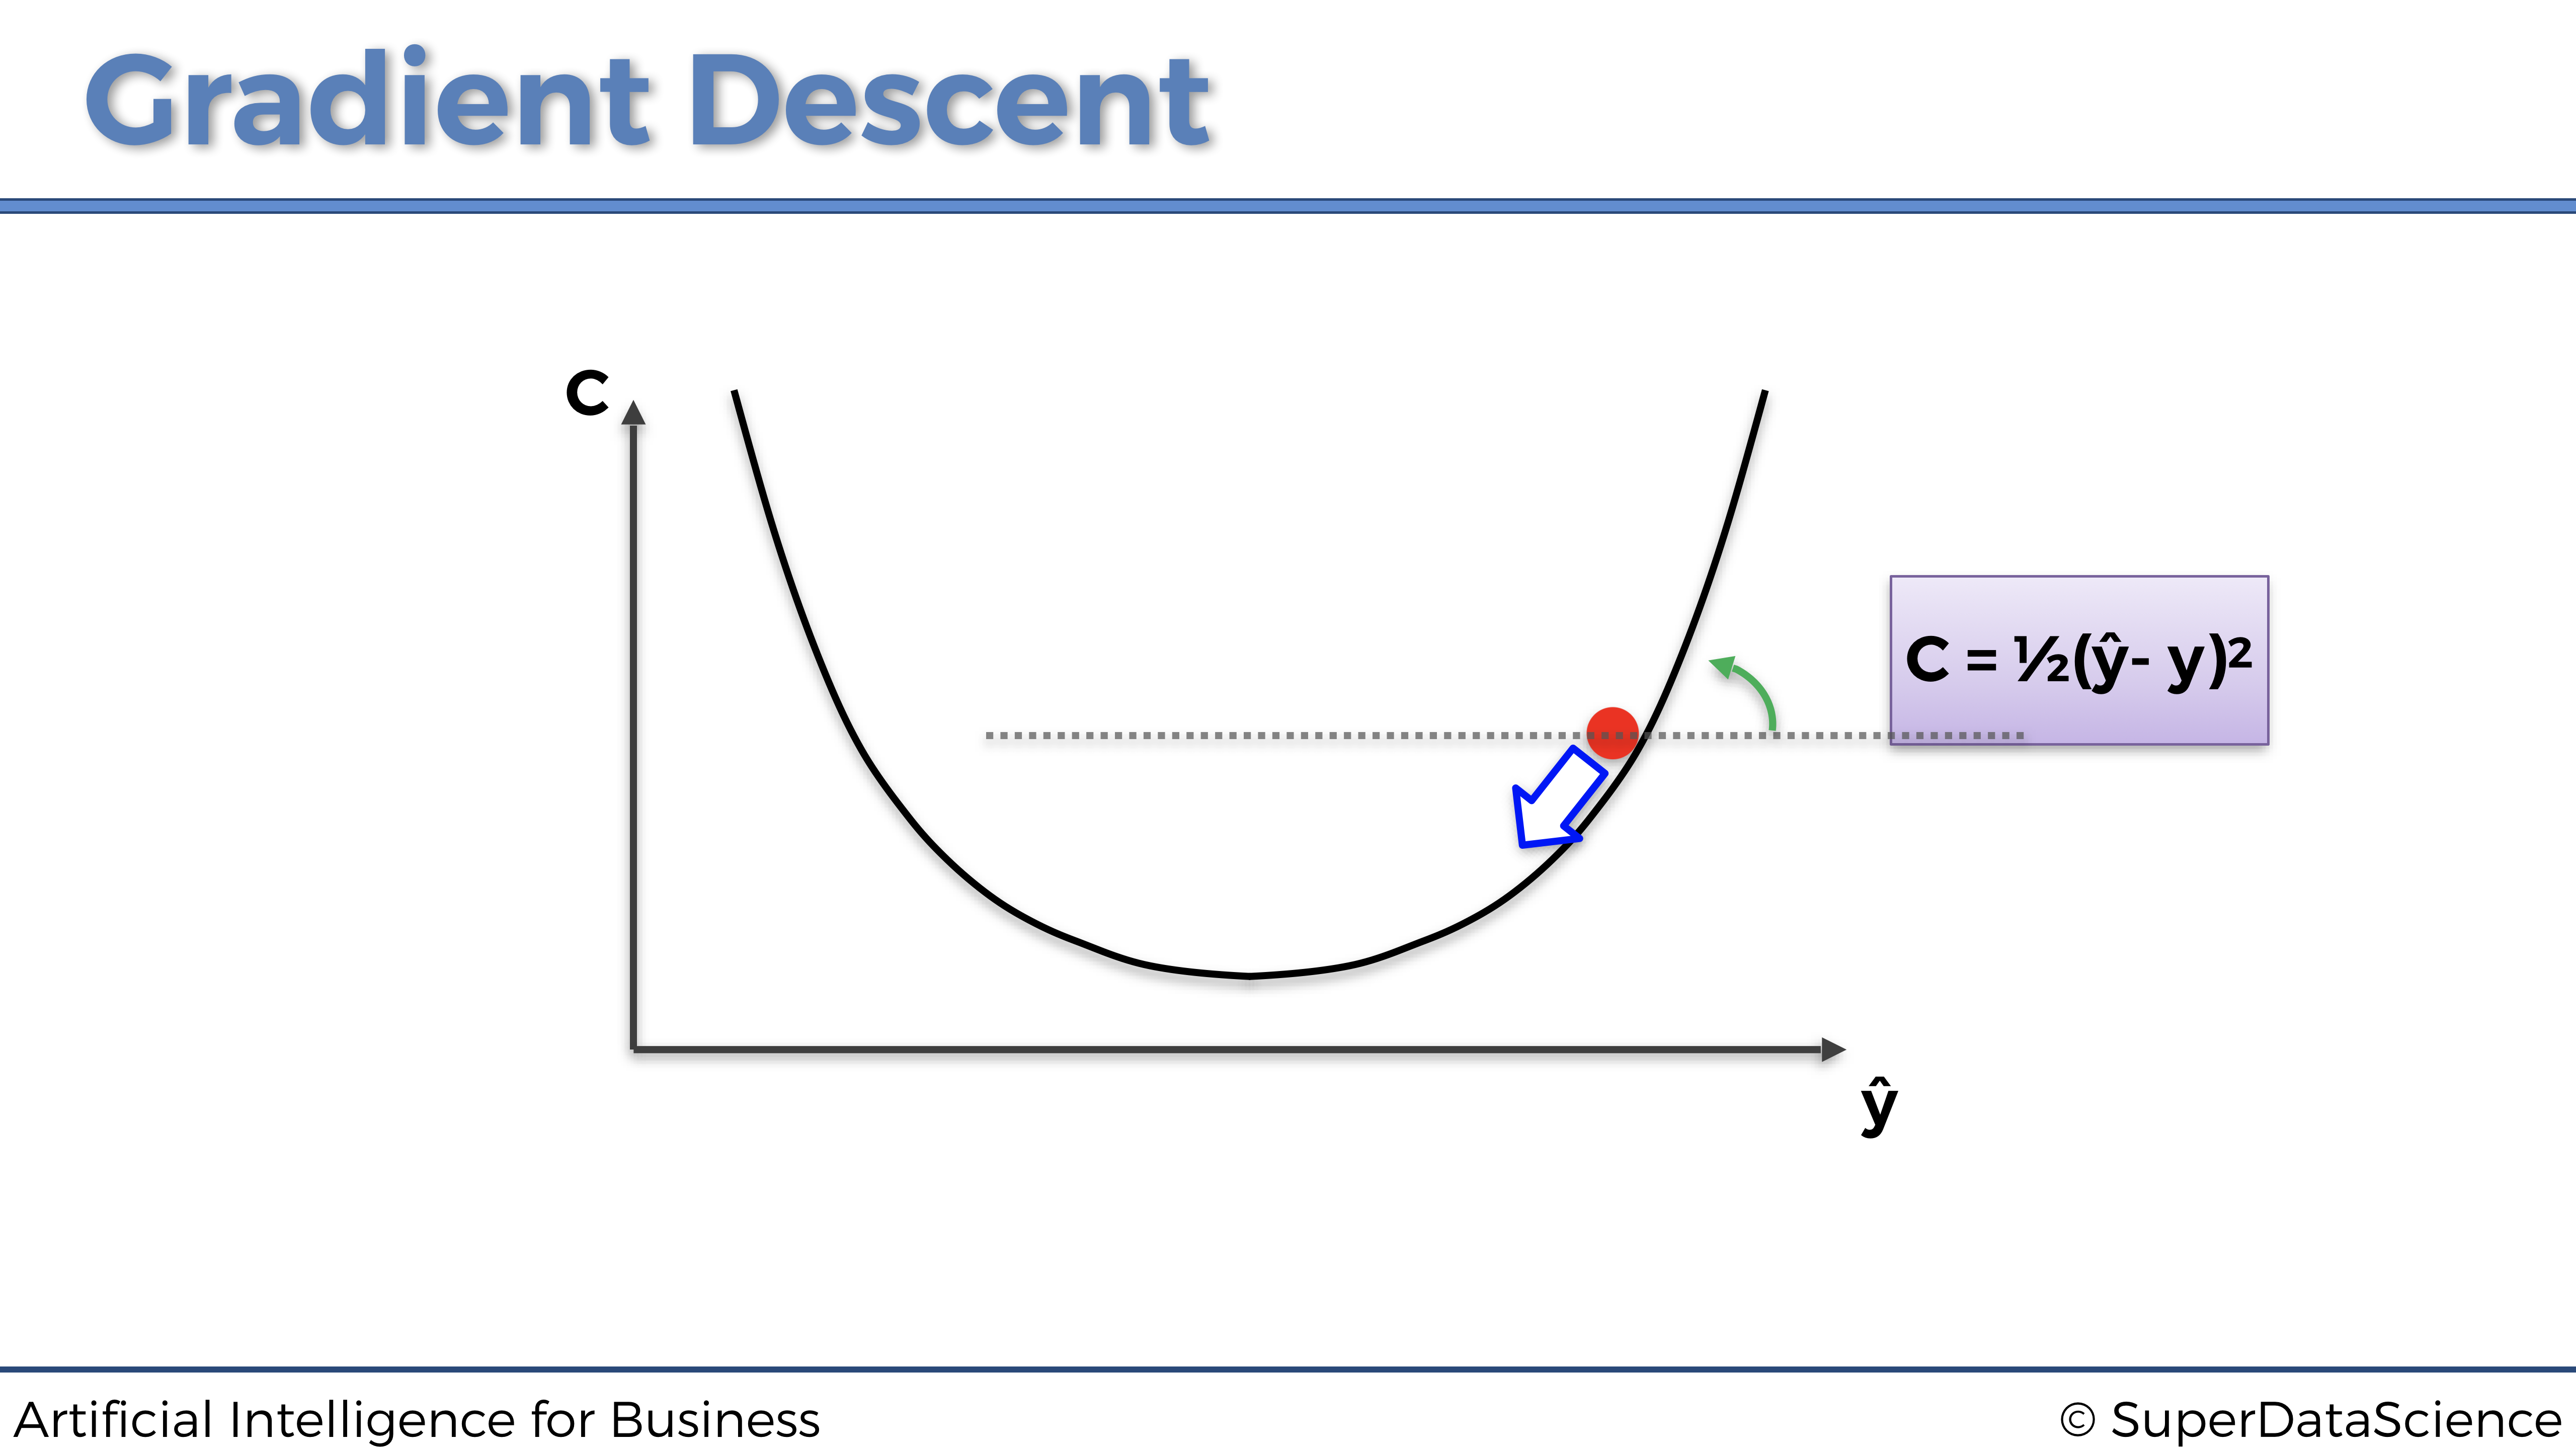
\includegraphics{Images/ANN_22.png}

Eventualmente, al repetir los mismos pasos, la pelota terminará en el fondo del bol:

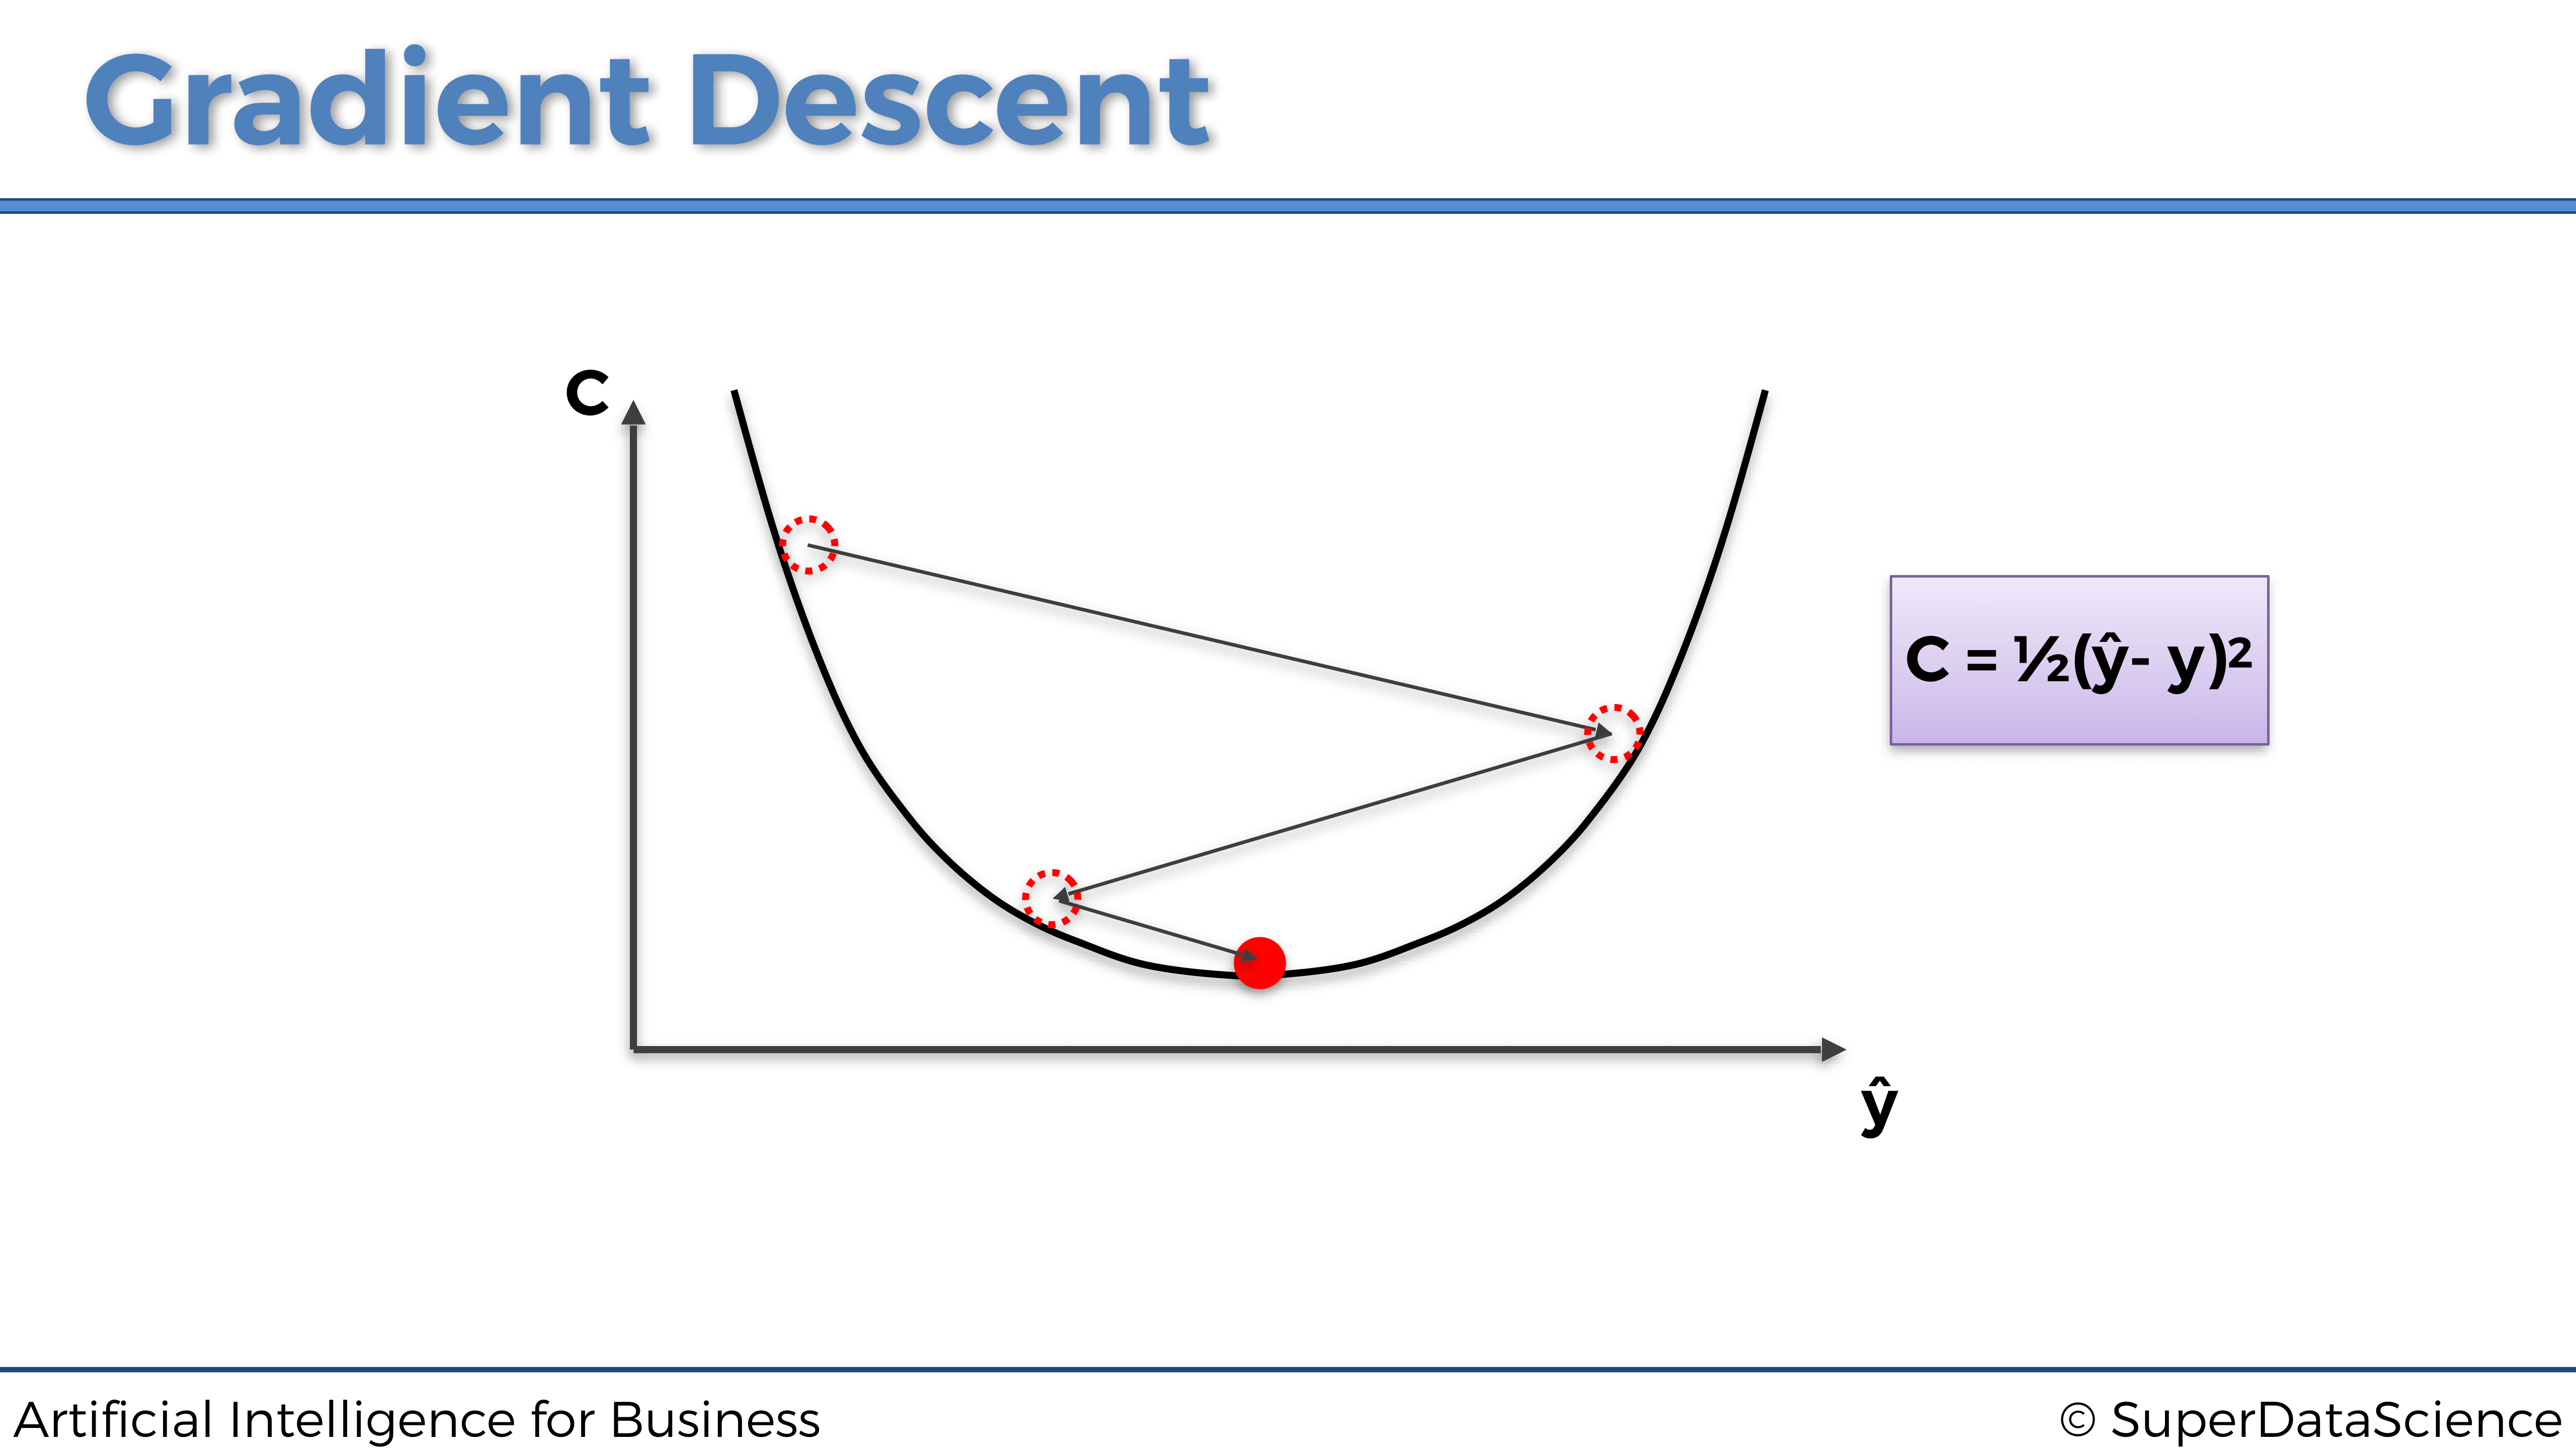
\includegraphics{Images/ANN_23.png}

¡Y eso es! Así es como el Gradiente Descendente opera en una dimensión (un parámetro). Ahora puedes preguntarte:

\begin{quote}
Genial, pero ¿cómo funciona esto a gran escala? Hemos visto un ejemplo de optimización unidimensional, ¿qué pasa con dos o incluso 3 dimensiones?
\end{quote}

Buena pregunta. El Gradiente Descendente garantiza que este enfoque se escala en tantas dimensiones como sea necesario, siempre que la función de costo sea convexa. De hecho, si la función de costo es convexa, el Gradiente Descendente encontrará siempre el mínimo \textbf{absoluto} de la función de costo. A continuación se muestra un ejemplo en 2 dimensiones:

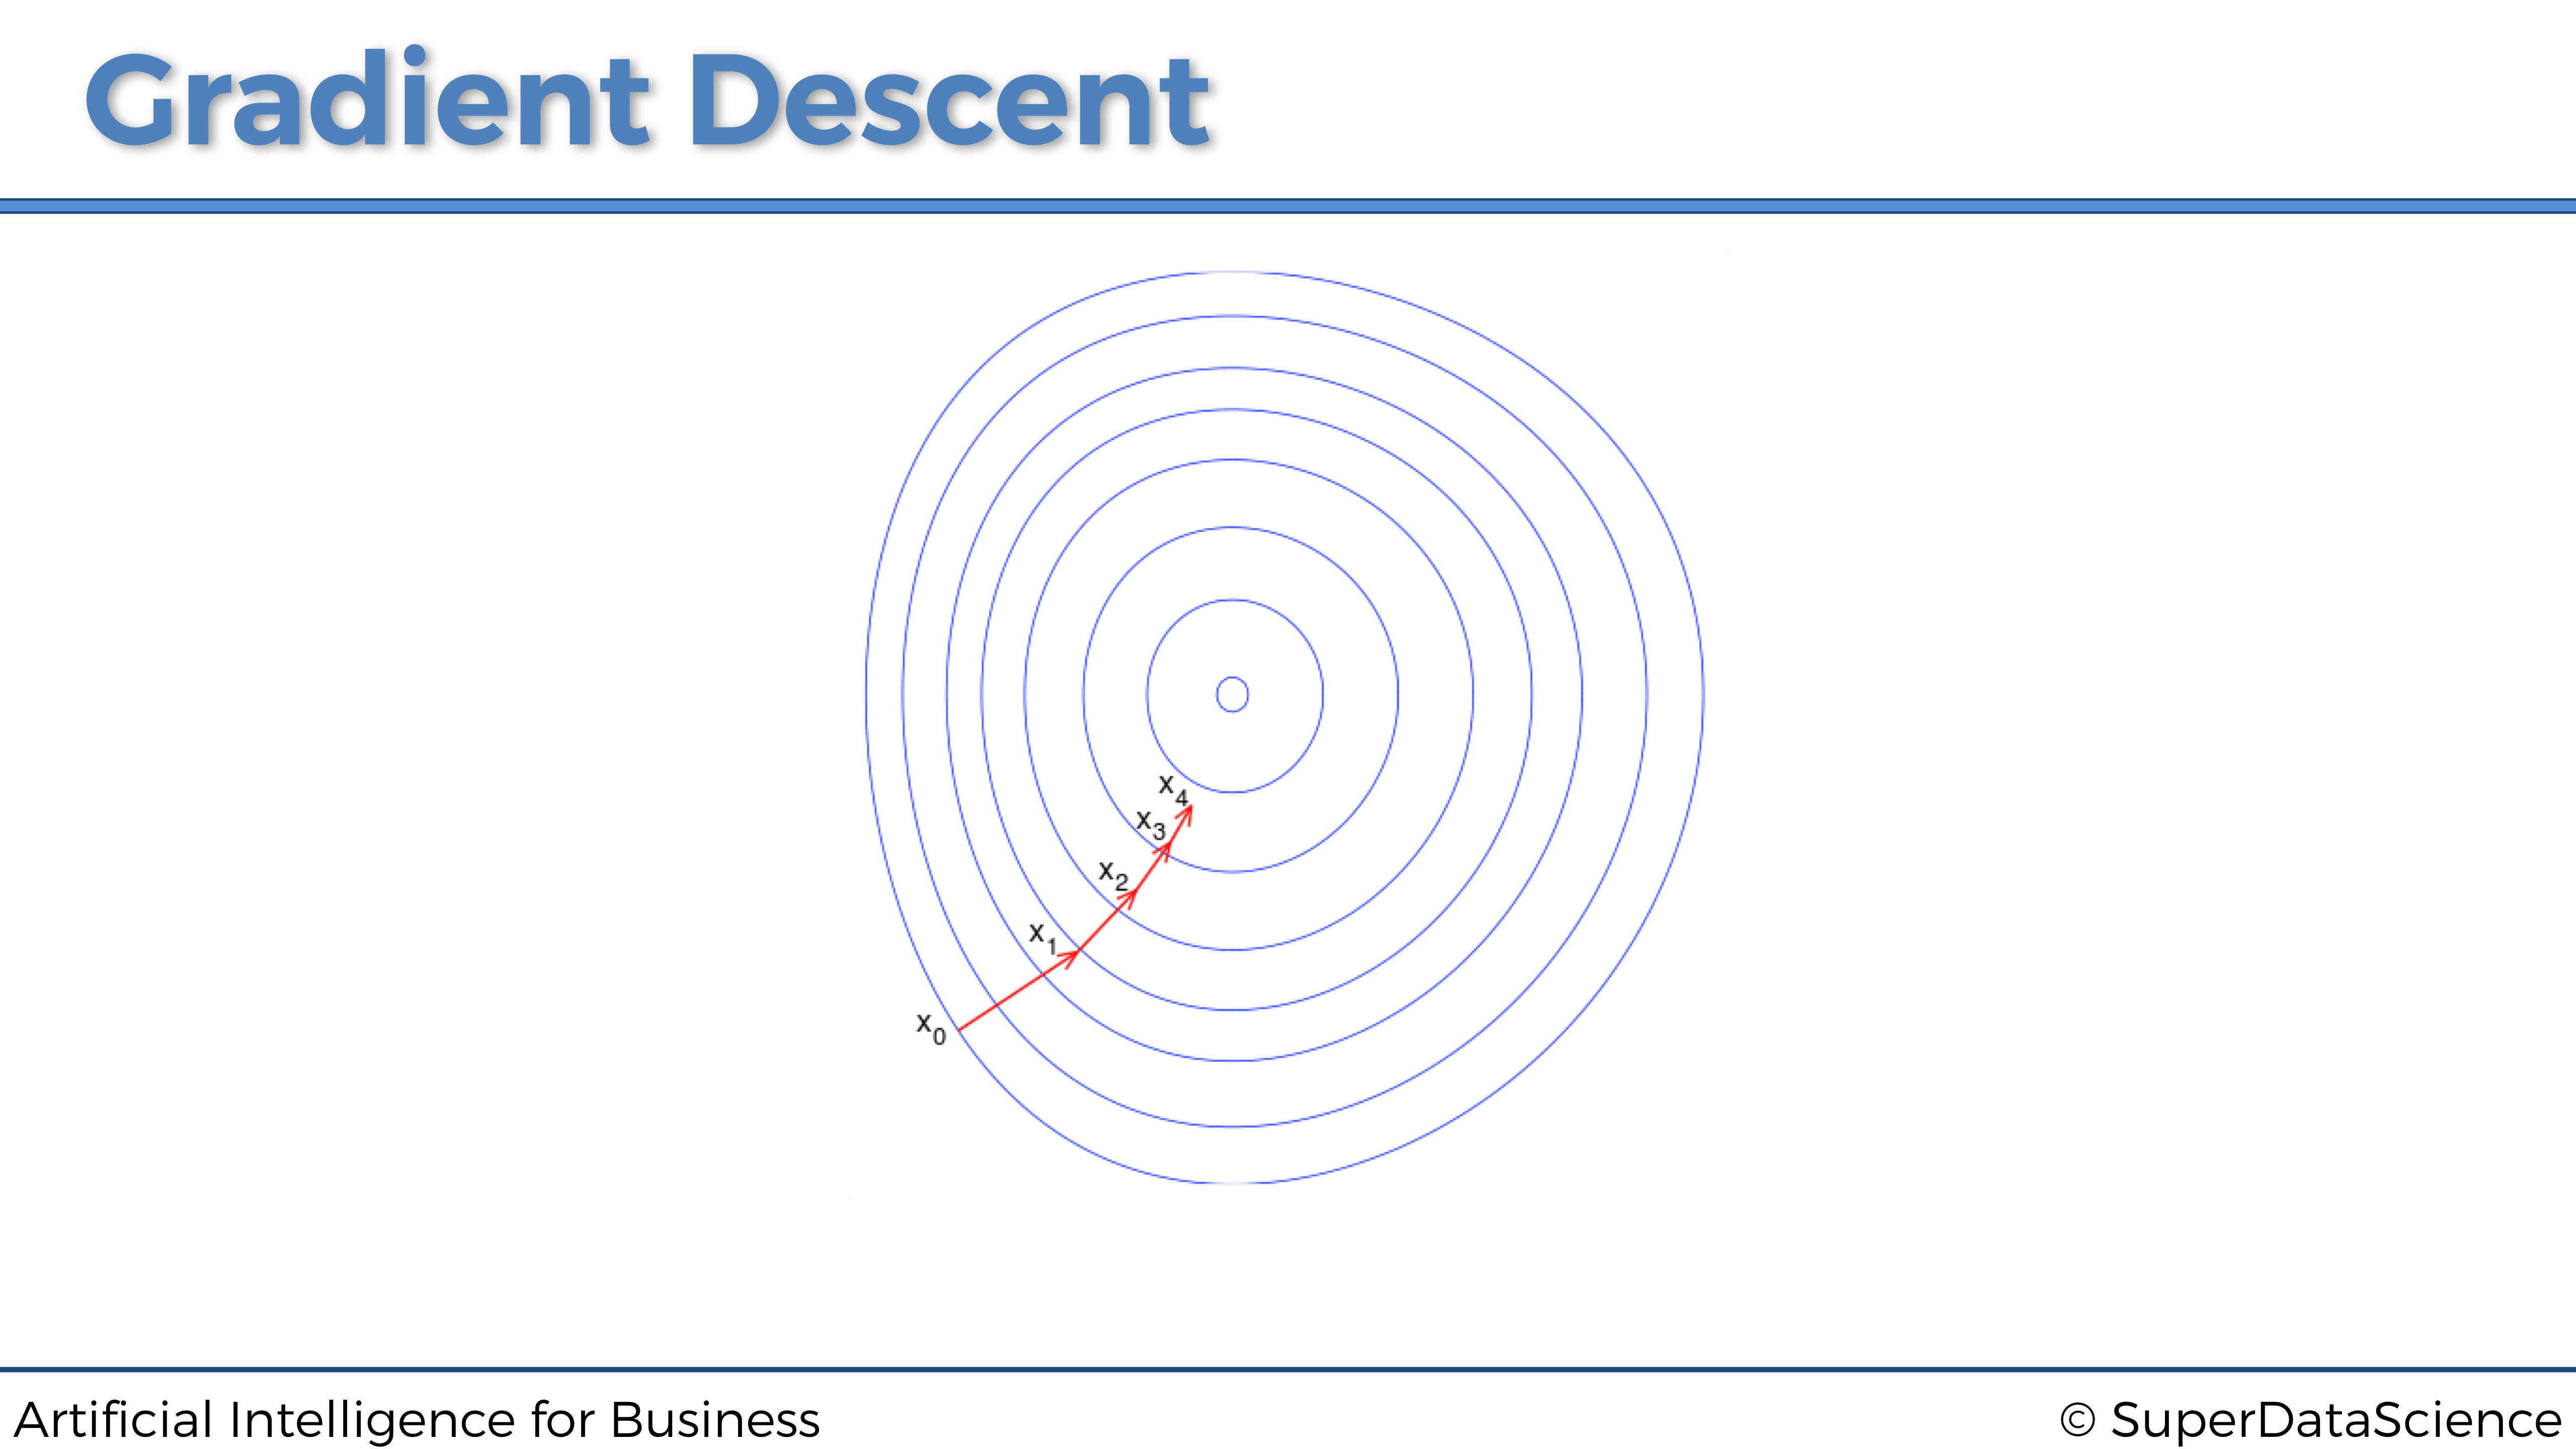
\includegraphics{Images/ANN_24.png}

Sin embargo, si la función de coste no es convexa, solo encontrará un mínimo \textbf{local}. A continuación se muestra un ejemplo en 3 dimensiones:

\includegraphics{Images/ANN_25.png}

Ahora que entendemos de qué se trata el gradiente descendente, es hora de estudiar las versiones más avanzadas y efectivas\ldots{}.

\begin{itemize}
\tightlist
\item
  Gradiente Descendente en bloques
\item
  Mini-Batch Gradiente Descendente
\item
  Stochastic Gradiente Descendente
\end{itemize}

\hypertarget{gradiente-descendente-en-bloques}{%
\subsubsection{Gradiente Descendente en bloques}\label{gradiente-descendente-en-bloques}}

``Gradiente Descendente'', ``Gradiente Descendente en Bloques'', ``Gradiente Descendente Mini Batch'', ``Gradiente Descendente Estocástico''.. Hay tantos términos y alguien que justo comienza a meterse en este mundillo puede encontrarlo muy confuso

La principal diferencia en todas estas versiones de Gradiente Descendente es la forma en que subministramos nuestros datos a un modelo y la frecuencia con la que actualizamos nuestros parámetros (pesos) para mover nuestra pequeña bola roja. Comencemos explicando el Gradiente Descendente en bloques.

Gradiente descendente en bloques es exactamente lo que hicimos en la Parte 2: Minimización de costes, donde recordemos que teníamos un lote de entradas que alimentaban la red neuronal, propagándolas hacia adelante para obtener al final un lote de predicciones, que a su vez se comparan con un lote de objetivos. El error de pérdida global entre las predicciones y los objetivos de los dos lotes se calcula como la suma de los errores de pérdida entre cada predicción y su objetivo asociado. Esa pérdida global se propaga nuevamente a la red neuronal, donde se realiza Gradiente Descendente o Gradiente Descendente estocástico para actualizar todos los pesos, de acuerdo con cómo fueron de responsables de ese error de pérdida global.

En la siguiente página a continuación hay un ejemplo de gradiente descendente en bloques. El problema a resolver es predecir la nota (de 0 a 100\%) que los estudiantes obtienen en un examen, en función del tiempo dedicado a estudiar y el tiempo dedicado a dormir:

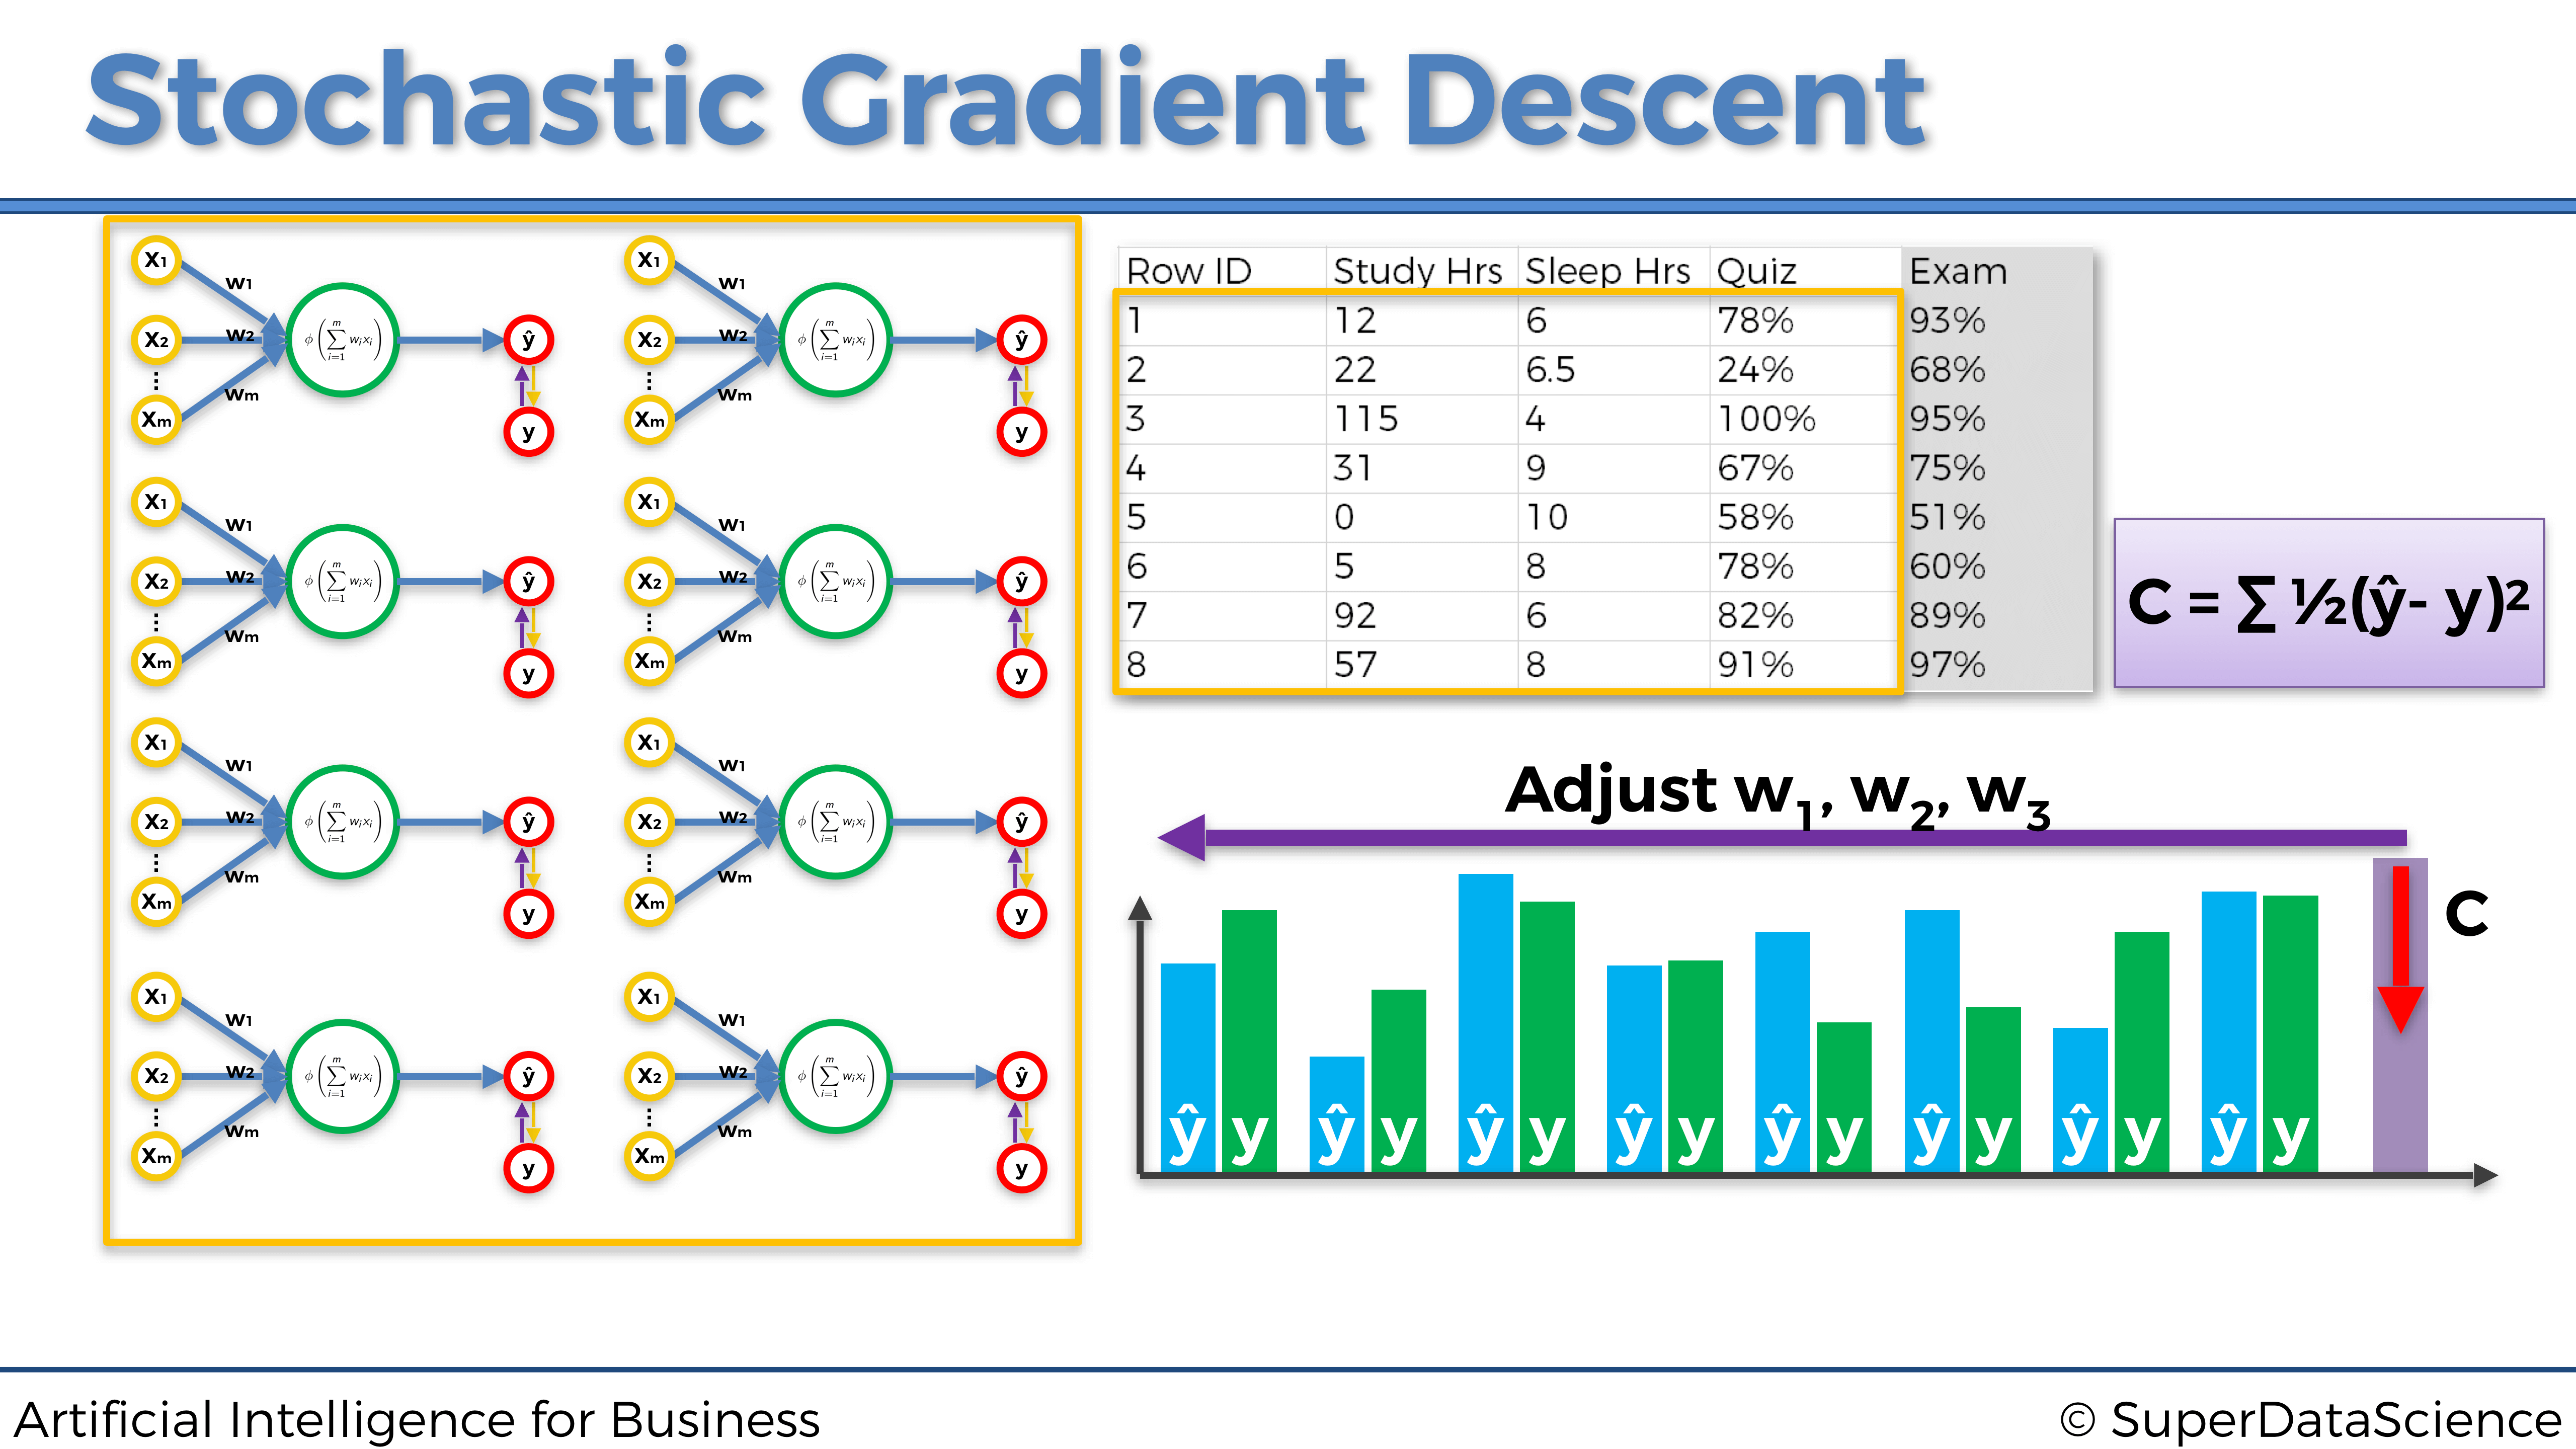
\includegraphics{Images/ANN_26.png}

Una cosa importante a tener en cuenta en este gráfico anterior es que estas no son redes neuronales múltiples, sino una sola representada por actualizaciones de peso separadas. Y nuevamente, como podemos notar que en este ejemplo de Gradiente Descendente en bloques, alimentamos todos nuestros datos al modelo a la vez. Esto producirá actualizaciones colectivas de los pesos y una rápida optimización de la red. Sin embargo, también está el lado malo de esto. Existe una vez más la posibilidad de quedarse atascado en un mínimo local, como podemos ver en el siguiente gráfico a continuación:

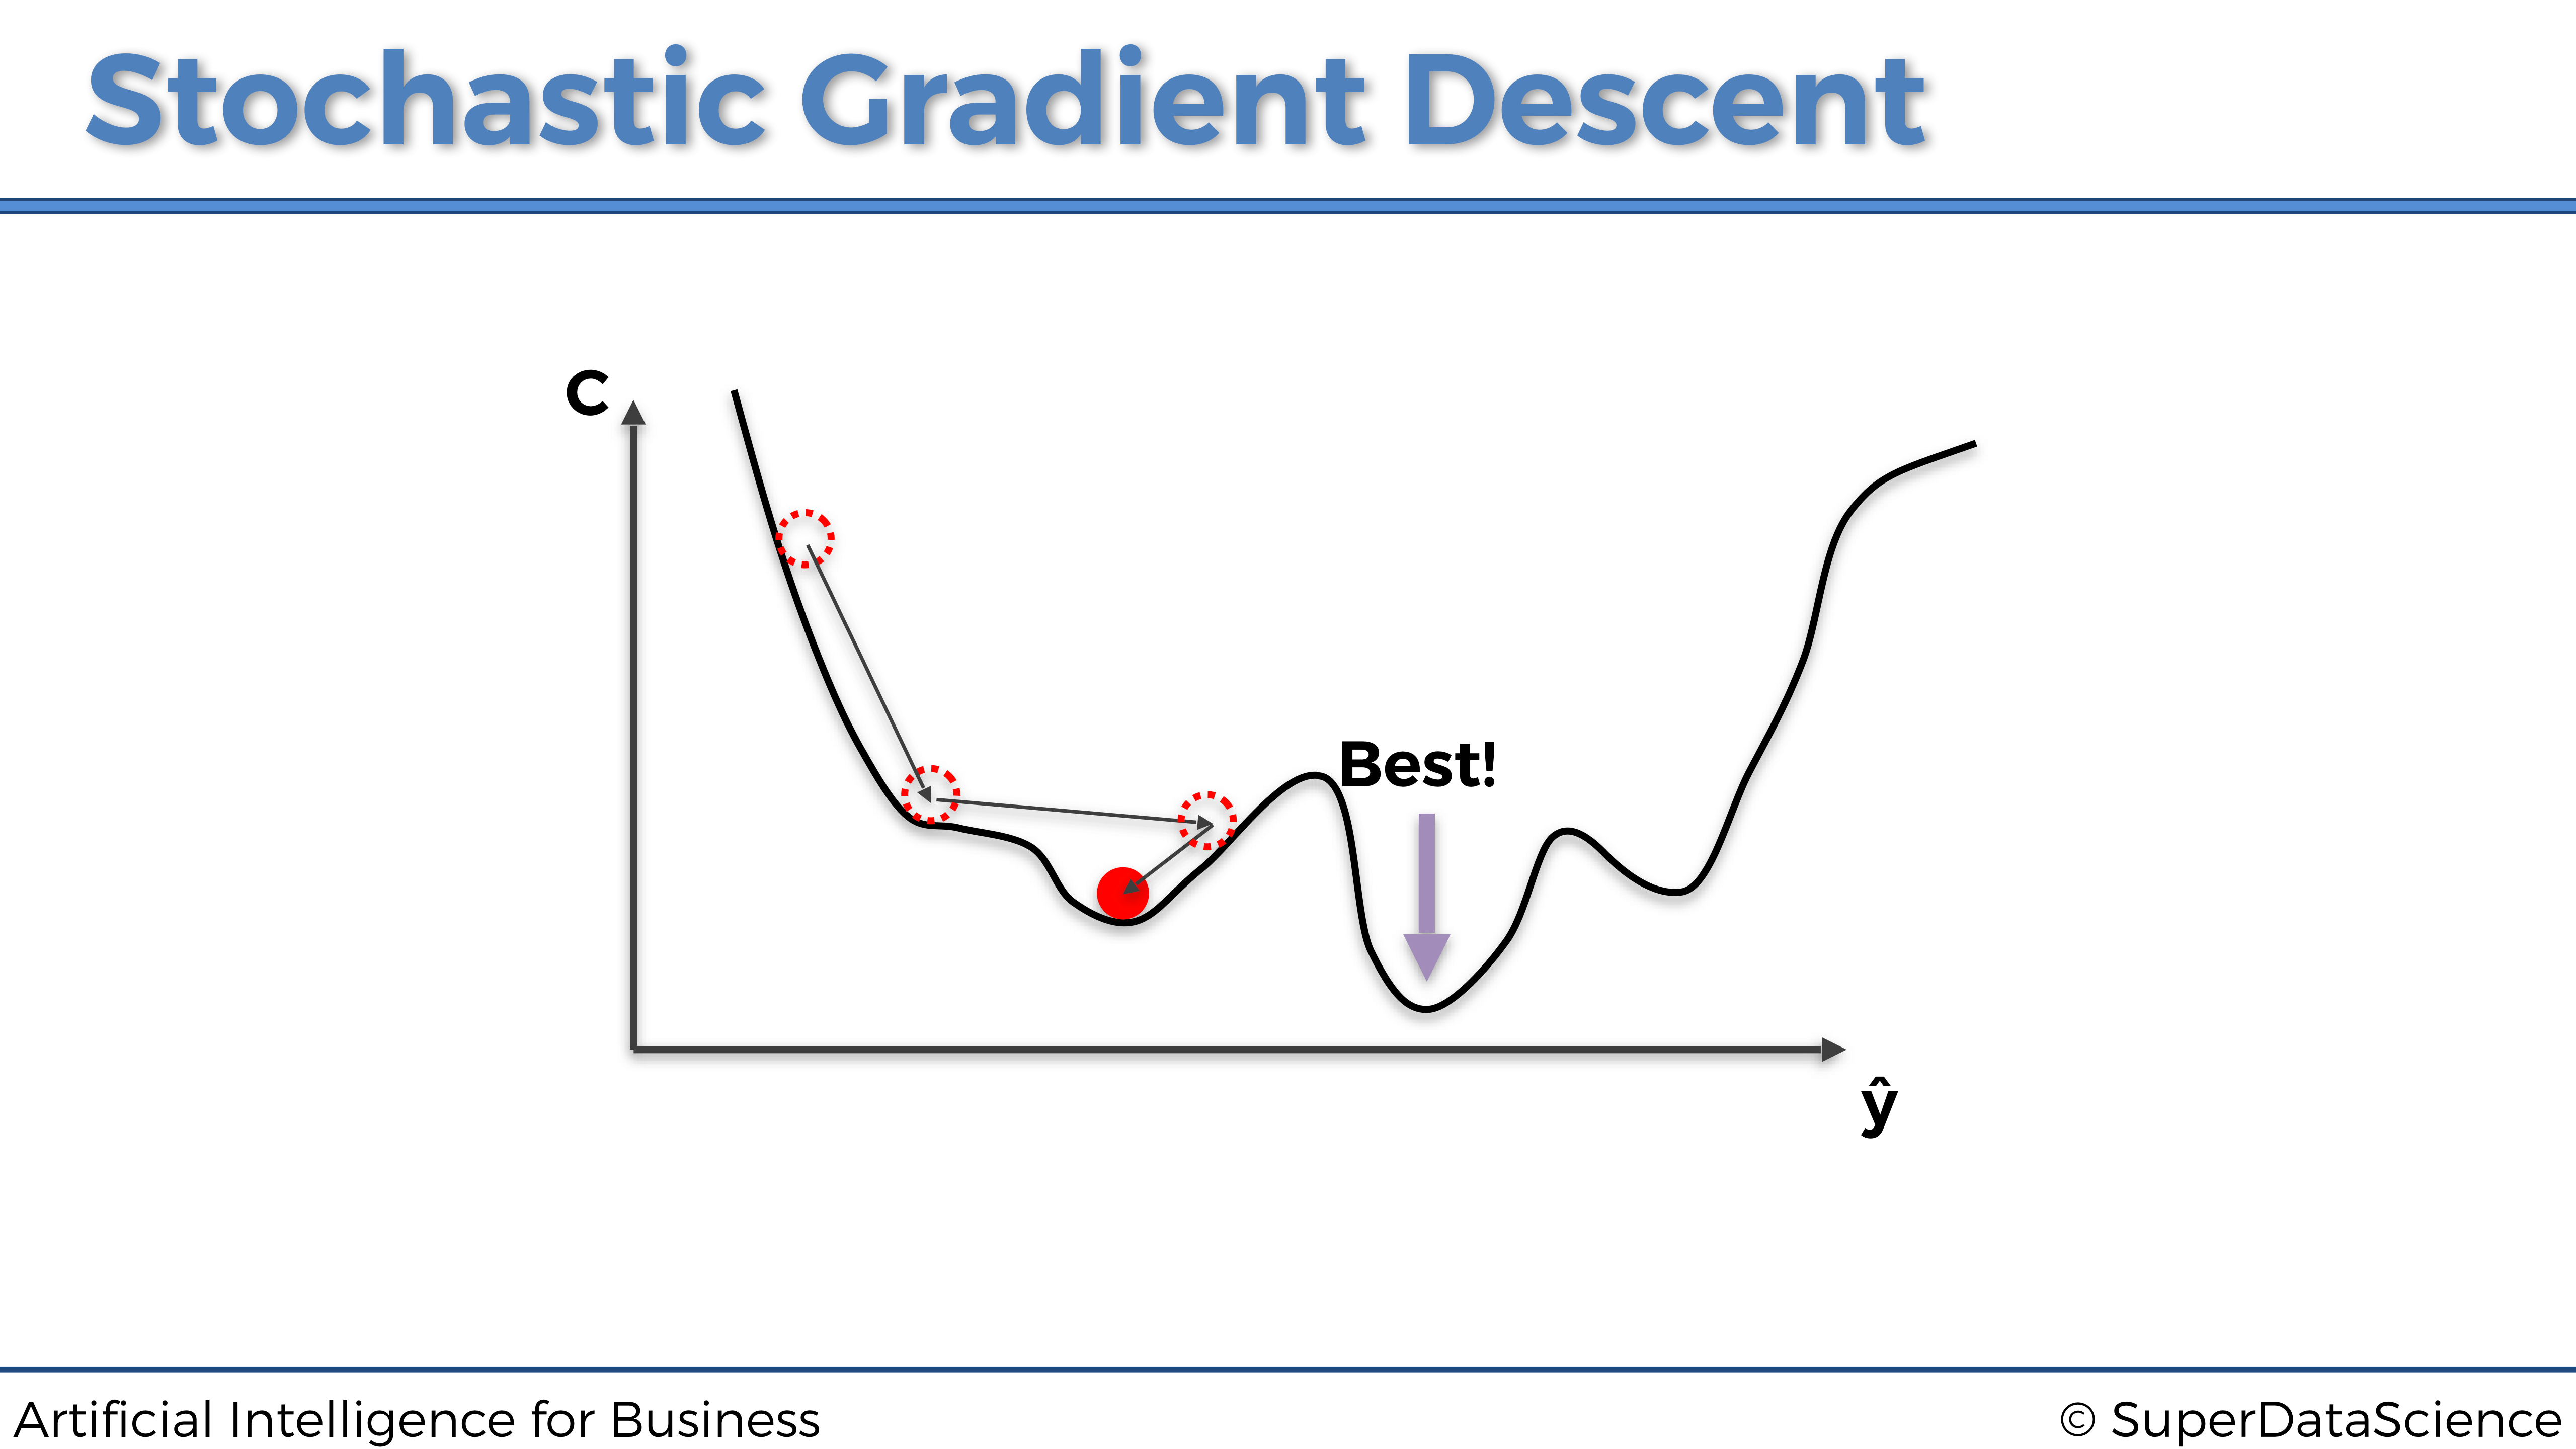
\includegraphics{Images/ANN_30.png}

La razón por la que esto sucede se ha explicado un poco antes: es porque la función de coste en el gráfico anterior no es convexa. Y este tipo de optimización (Gradiente Descendente simple) requiere que la función de costo sea convexa. Si ese no es el caso, podemos encontrarnos atrapados en un mínimo local y nunca encontrar el mínimo global que tenga los parámetros óptimos. Por otro lado, a continuación se muestra un ejemplo de una función de coste convexa, la misma que vimos anteriormente:

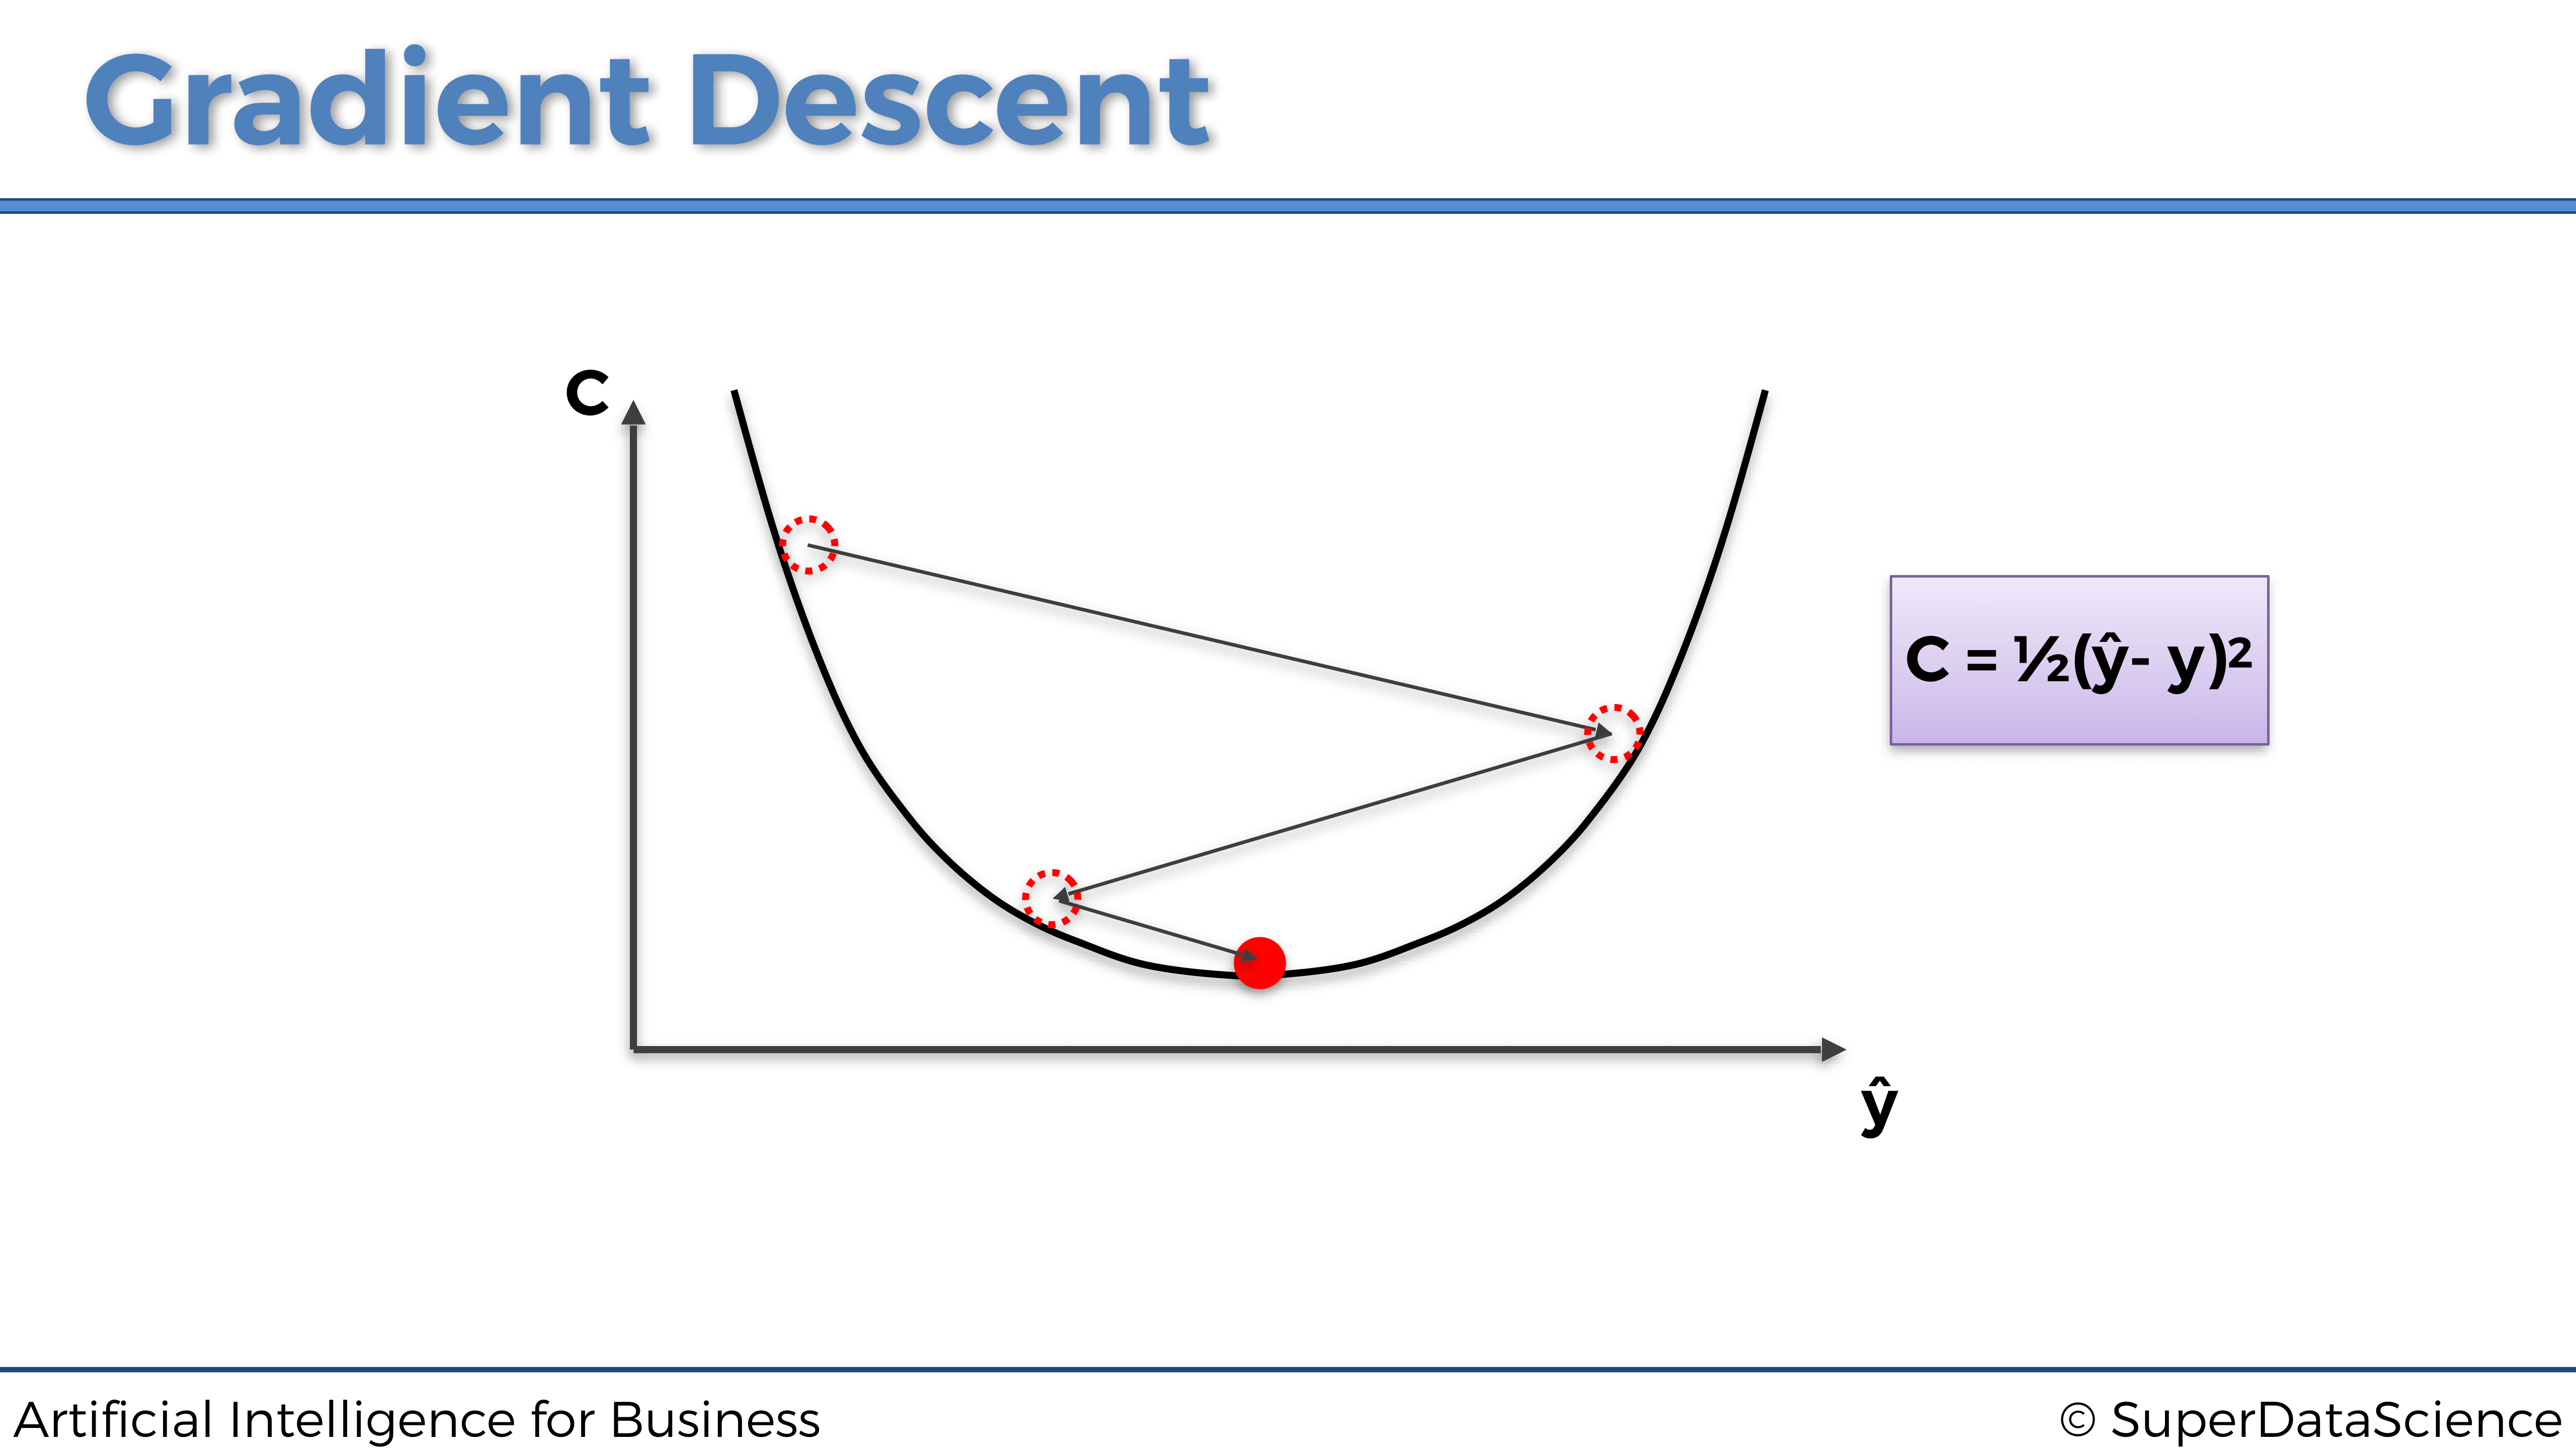
\includegraphics{Images/ANN_23.png}

En pocas palabras, una función es convexa si solo tiene un mínimo global. Y el gráfico de una función convexa tiene la forma del bol.

Sin embargo, en la mayoría de los problemas, incluidos los problemas comerciales, la función de coste no será convexa (como en este mismo ejemplo gráfico en 3D a continuación), por lo que no permite que Gradiente Descendente funcione correctamente. Aquí es donde entra en juego el Gradiente Descendente Estocástico.

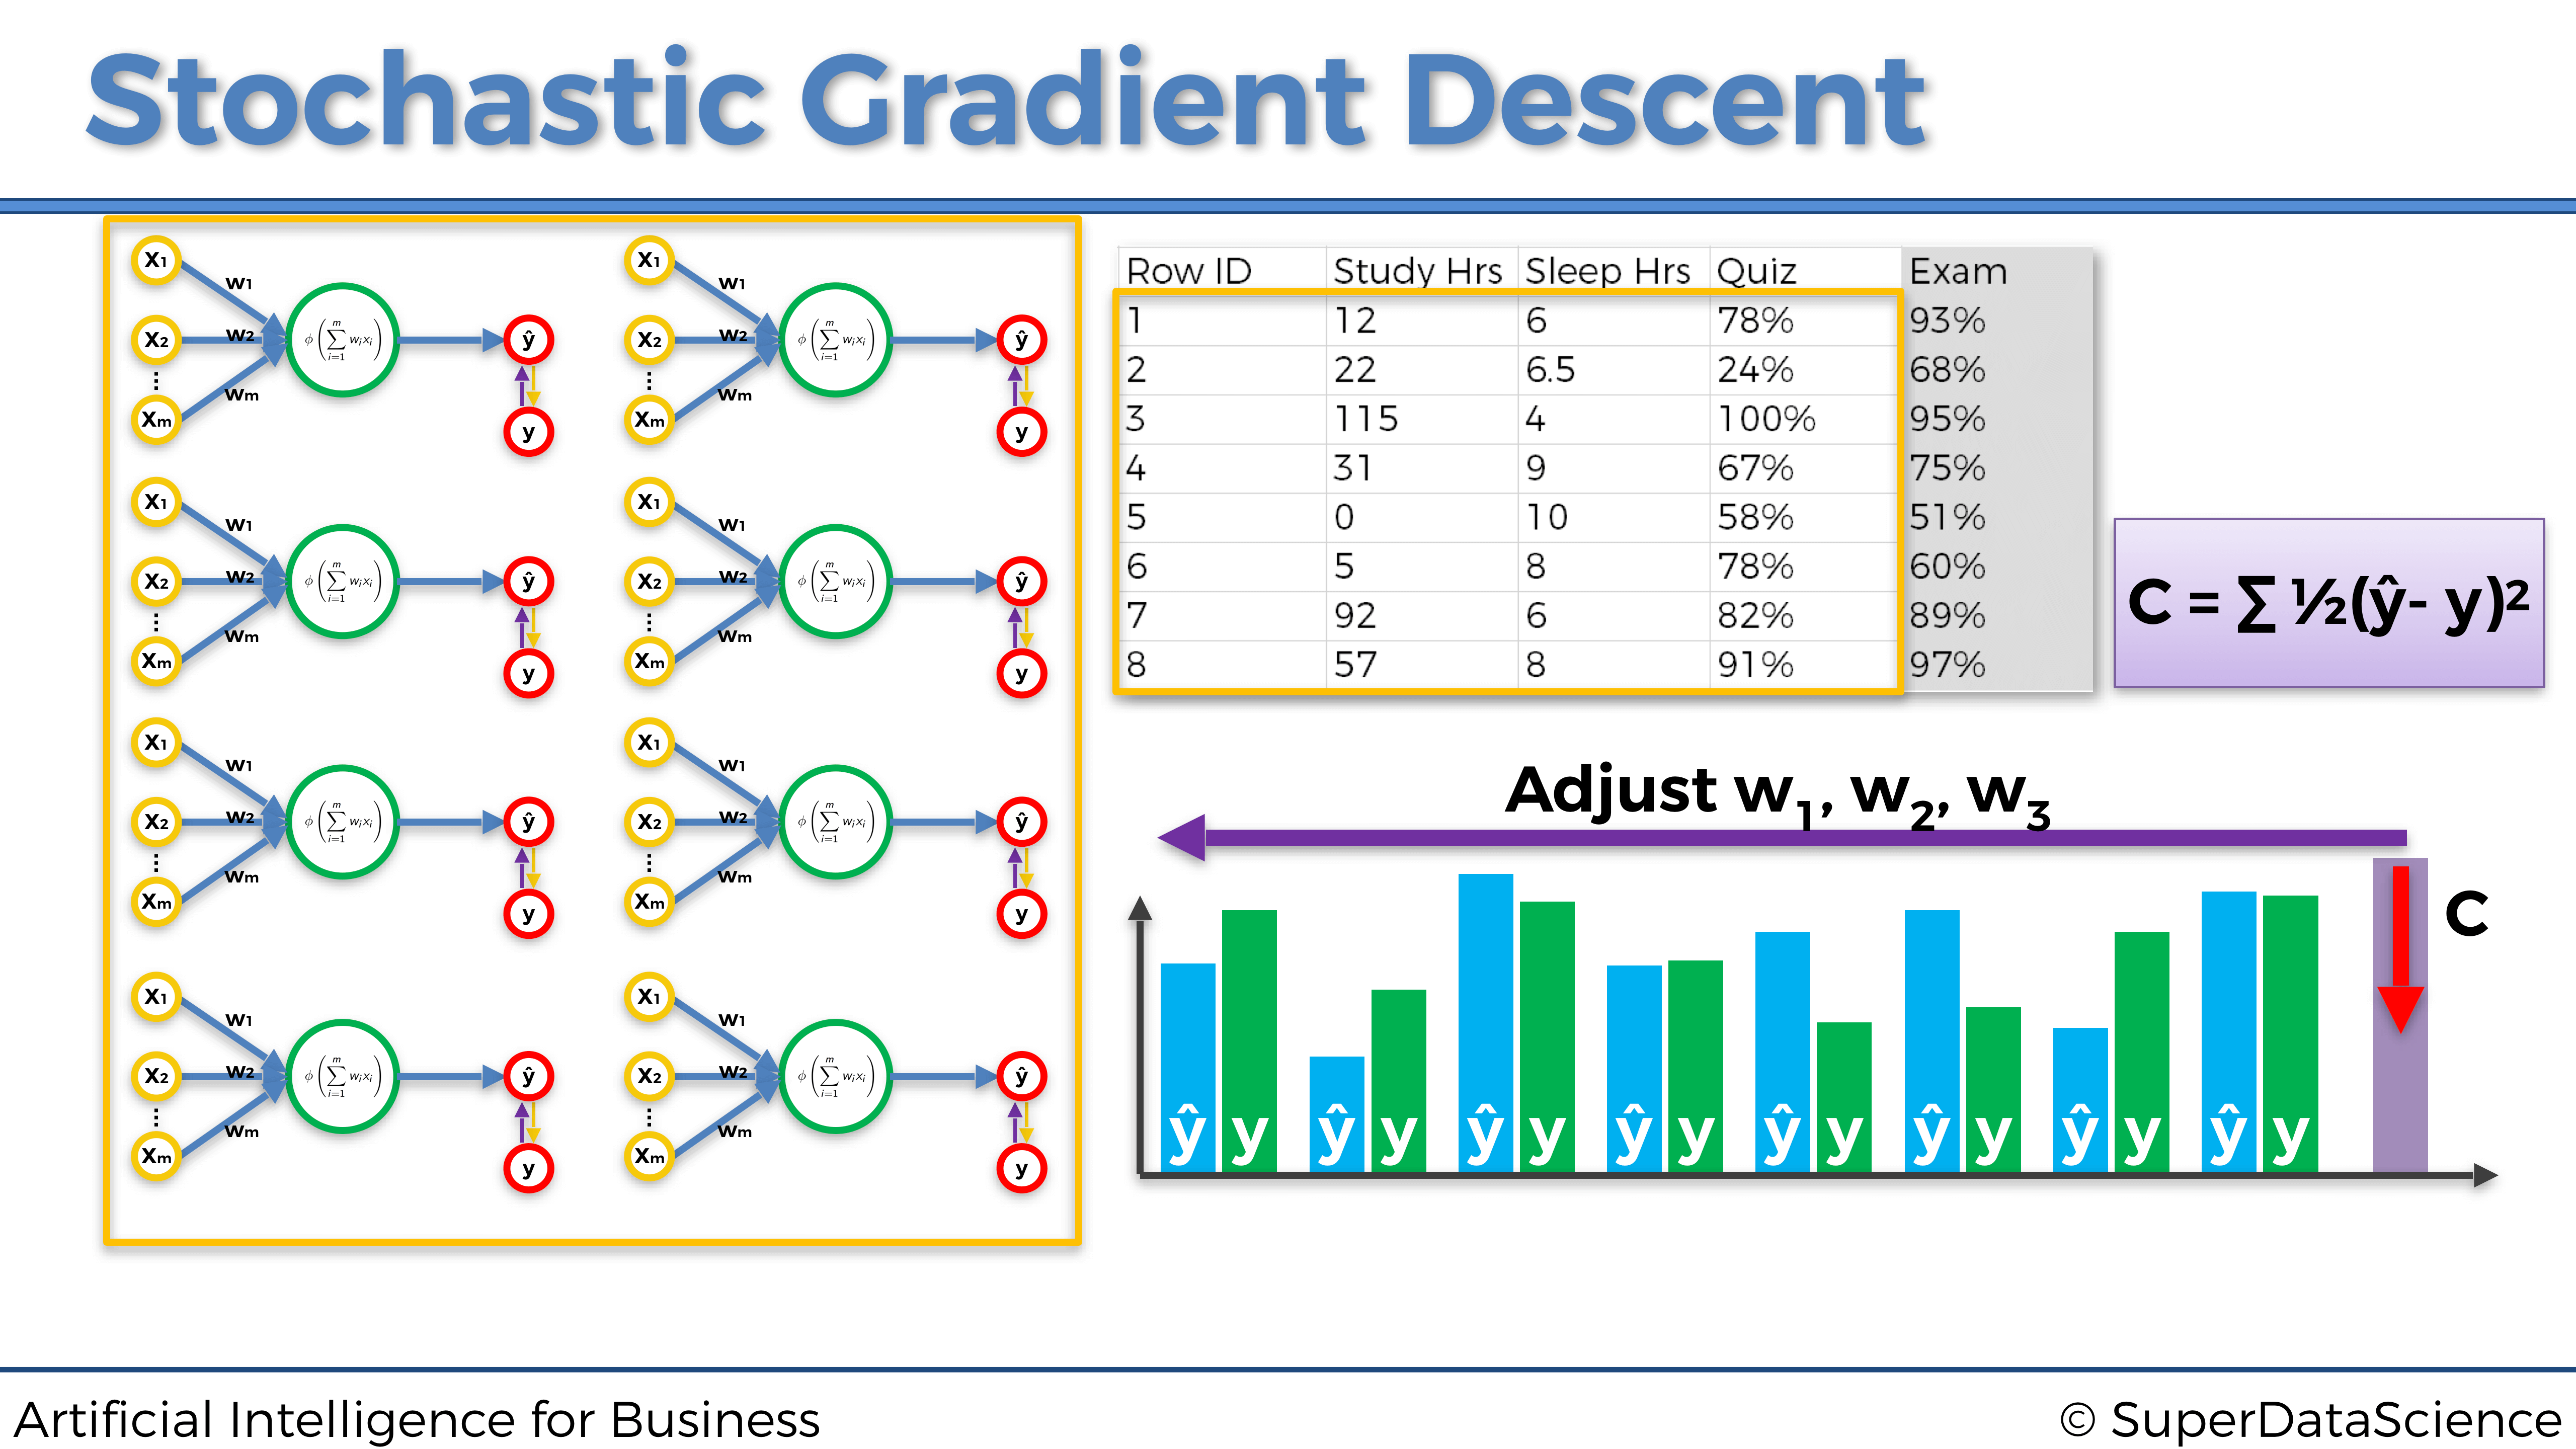
\includegraphics{Images/ANN_26.png}

\hypertarget{gradiente-descendente-estocuxe1stico}{%
\subsubsection{Gradiente Descendente Estocástico}\label{gradiente-descendente-estocuxe1stico}}

Gradiente Descendente Estocástico (SGD) viene a salvarnos de la catástrofe anterior. De hecho, proporciona mejores resultados en general, evitando que el algoritmo se atasque en un mínimo local. Sin embargo, como su nombre lo indica, es estocástico, o en otras palabras, aleatorio. Debido a esta propiedad, no importa cuántas veces ejecutemos el algoritmo, el proceso siempre será ligeramente diferente. Y eso, independientemente de la inicialización.

El Gradiente Descendente Estocástico no se ejecuta sobre todo el conjunto de datos a la vez, sino que se introducen las entradas una a una. Por lo tanto, el proceso es así:

\begin{enumerate}
\def\labelenumi{\arabic{enumi}.}
\tightlist
\item
  Se introduce una sola observación
\item
  Se obtiene una única predicción
\item
  Se calcula el error de pérdida entre la predicción y el objetivo
\item
  Se vuelve a propagar el error de pérdida en la red neuronal
\item
  Se actualizan los pesos con Gradiente Descendente
\item
  Se repiten los pasos 1. a 5. a través de todo el conjunto de datos
\end{enumerate}

Representemos las tres primeras iteraciones en las tres primeras entradas individuales para este mismo ejemplo dado anteriormente sobre la predicción de las puntuaciones en un examen:

\textbf{Primera fila de entrada de observación}:

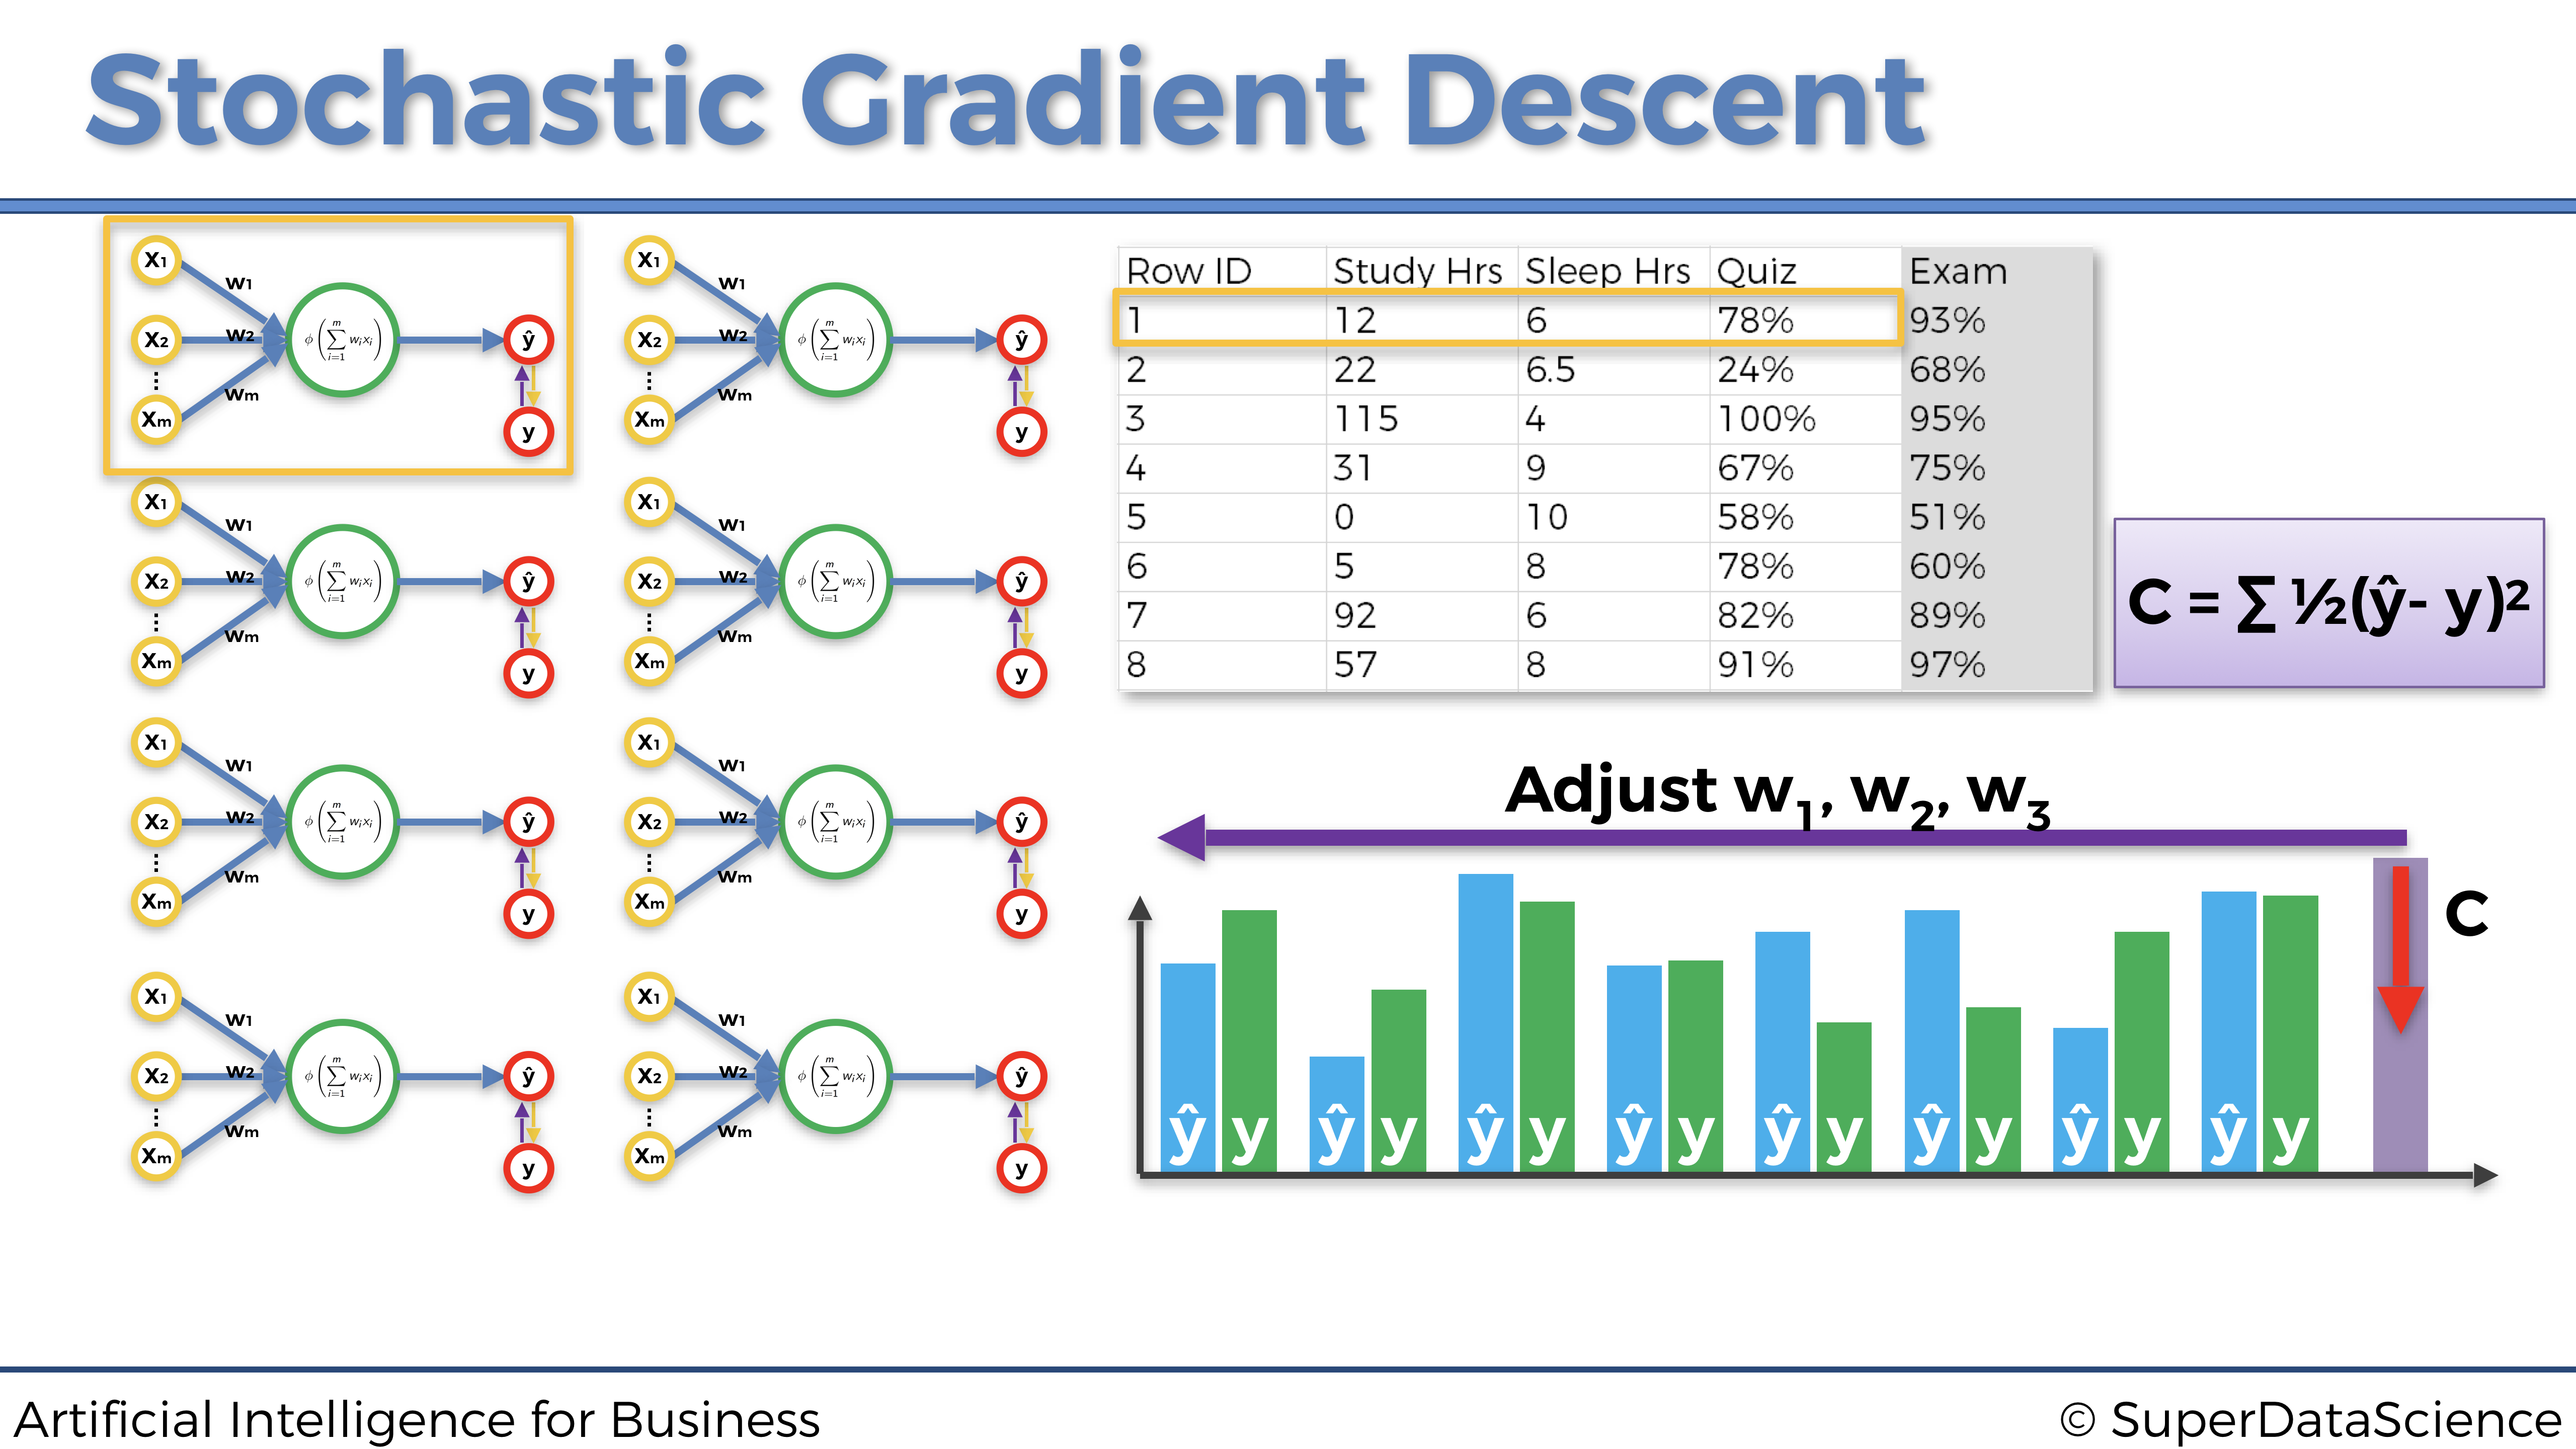
\includegraphics{Images/ANN_27.png}

\textbf{Segunda fila de entrada de observación}:

\includegraphics{Images/ANN_28.png}

\textbf{Tercera fila de entrada de observación}:

\includegraphics{Images/ANN_29.png}

Cada uno de los tres gráficos anteriores es un ejemplo de una actualización de pesos ejecutada por el Gradiente Descendente Estocástico. Como podemos ver, cada vez introducimos una sola fila de observación desde nuestro conjunto de datos a la red neuronal, luego actualizamos los pesos en consecuencia y procedemos a la siguiente fila de entrada de observación.

A primera vista, el gradiente descendente estocástico parece más lento, porque introducimos cada fila por separado. Pero en realidad, es mucho más rápido debido al hecho de que no tenemos que cargar todo el conjunto de datos en la memoria, ni esperar a que todo el conjunto de datos pase por el modelo actualizando los pesos.

Para finalizar esta sección, repasemos la diferencia entre gradiente descendente en bloque y gradiente descendente estocástico, con el siguiente gráfico:

\includegraphics{Images/ANN_31.png}

\hypertarget{gradiente-descendente-mini-batch}{%
\subsubsection{Gradiente Descendente Mini-Batch}\label{gradiente-descendente-mini-batch}}

El Gradiente Descendente Mini-Batchutiliza lo mejor de ambos mundos para combinar gradiente descendente en bloques con el dradiente descendente estocástico. Esto se hace alimentando la red neuronal con lotes de datos en lugar de alimentar filas de observaciones individuales una por una o todo el conjunto de datos a la vez.

Este enfoque es más rápido que el Gradiente Descendente Estocástico clásico y evita que se atasque en un mínimo local. Esto también ayuda cuando las personas no tienen suficientes recursos informáticos para cargar todo el conjunto de datos en la memoria, o suficiente potencia de procesamiento para obtener el beneficio completo del Gradiente Descendente Estocástico.

\hypertarget{optimizadores}{%
\subsection{Optimizadores}\label{optimizadores}}

El optimizador es exactamente la herramienta que actualizará los pesos de la red neuronal a través del gradiente estocástico descendente. Hasta este punto, solo hemos mencionado el optimizador Adam (consulta la Parte 2: Minimización de costos), que es el optimizador más común utilizado para los modelos de Aprendizaje profundo y Aprendizaje por refuerzo profundo. Sin embargo, hay muchos más optimizadores que tienen sus propios beneficios y aplicaciones.

Veamos los optimizadores de gradiente descendente más famosos y ampliamente utilizados.

\hypertarget{optimizador-momentum}{%
\subsubsection{Optimizador Momentum}\label{optimizador-momentum}}

El Gradiente Descendente Estocástico clásico tiene oscilaciones muy grandes, lo que deja margen de mejora. El optimizador Momentum (también llamado optimizador de impulso) maneja estas grandes oscilaciones agregando fracciones de las direcciones calculadas en el paso anterior al paso actual. Esto amplifica la velocidad de la actualización de dirección actual. En el gráfico a continuación podemos ver y comparar el SGD clásico y el SGD Momentum en acción:

\includegraphics{Images/ANN_32.png}

Los beneficios de optimizador Momentum son los siguientes:

\begin{itemize}
\tightlist
\item
  Convergencia más rápida
\item
  Menos oscilaciones
\end{itemize}

Pero el optimizador Momentum también tiene inconvenientes, que son los siguientes:

\begin{itemize}
\tightlist
\item
  Tendencia a sobrepasar el mínimo global de la función de coste debido al impulso.
\item
  Menos frecuente en las librerías de Deep Learning, lo que requiere el conocimiento adicional de programación para su implementación.
\end{itemize}

\hypertarget{el-optimizador-de-gradiente-acelerado-de-nesterov}{%
\subsubsection{El optimizador de gradiente acelerado de Nesterov}\label{el-optimizador-de-gradiente-acelerado-de-nesterov}}

Yuri Nesterov resolvió el problema de sobrepasar el mínimo global del optimizador Momentum invirtiendo el orden de cálculo en la fórmula de actualización:

\includegraphics{Images/ANN_33.png}

\hypertarget{el-optimizador-adagrad-gradientes-adaptativos}{%
\subsubsection{El optimizador AdaGrad (gradientes adaptativos)}\label{el-optimizador-adagrad-gradientes-adaptativos}}

La idea de adaptar nuestras actualizaciones de acuerdo con la pendiente de la función de error, proveniente del optimizador de Nesterov, se toma y aplica en el optimizador AdaGrad al tiempo que se optimiza también la tasa de aprendizaje.

Por lo tanto, en el optimizador AdaGrad tenemos el mismo principio, no solo aplicado en gradientes sino también en la tasa de aprendizaje.

Estos son los beneficios de este optimizador:

\begin{itemize}
\tightlist
\item
  El optimizador AdaGrad permite realizar grandes actualizaciones para parámetros poco frecuentes.
\item
  Y permite realizar pequeñas actualizaciones para parámetros frecuentes.
\end{itemize}

Y aquí están los inconvenientes:

\begin{itemize}
\tightlist
\item
  La tasa de aprendizaje siempre disminuye, y esto podría llevar a actualizaciones muy pequeñas, si es que las hay.
\item
  Es menos frecuente en las librerías de Deep Learning, lo que requiere el conocimiento necesario para su implementación.
\end{itemize}

\hypertarget{el-optimizador-adadelta}{%
\subsubsection{El optimizador AdaDelta}\label{el-optimizador-adadelta}}

El AdaDelta Optimizer se inventó para corregir ese problema de disminución de la tasa de aprendizaje del optimizador AdaGrad ( el primer inconveniente anterior). No es necesario dar más detalles, solo necesitamos presentar el optimizador AdaDelta y su particularidad para comprender la fortaleza del optimizador más utilizado y más eficaz: el optimizador Adam

\hypertarget{el-optimizador-adam-adaptive-moment-estimation}{%
\subsubsection{El optimizador Adam (Adaptive Moment Estimation)}\label{el-optimizador-adam-adaptive-moment-estimation}}

El optimizador Adam es una mejora enorme con respecto al AdaDelta. La idea detrás de esto es almacenar en una memoria los cambios de impulso, ya que calculamos la tasa de aprendizaje para cada parámetro por separado.

Conviene recordar bien los beneficios del optimizador Adam, que deben tenerse en cuenta al construir una red neuronal.

\begin{itemize}
\tightlist
\item
  Es uno de los optimizadores más potentes.
\item
  Viene implementado de serie en la mayoría de librerías de Deep Learning (Keras, TensorFlow, PyTorch). No lo echarás en falta.
\end{itemize}

Por supuesto, este es el que usamos al construir el Cerebro Artificial de nuestra IA en la Parte 2 - Minimización de los costes. Veamos nuevamente el código que construye este cerebro artificial y notemos, en la última línea de código, la simplicidad de seleccionar el Adam Optimizer al crearlo:

\begin{Shaded}
\begin{Highlighting}[]
\CommentTok{# Inteligencia Artificial aplicada a Negocios y Empresas - Caso Práctico 2}
\CommentTok{# Construcción del cerebro}

\CommentTok{# Importar las librerías}
\ImportTok{from}\NormalTok{ keras.layers }\ImportTok{import}\NormalTok{ Input, Dense}
\ImportTok{from}\NormalTok{ keras.models }\ImportTok{import}\NormalTok{ Model}
\ImportTok{from}\NormalTok{ keras.optimizers }\ImportTok{import}\NormalTok{ Adam}

\CommentTok{# CONSTRUCCIÓN DEL CEREBRO}

\KeywordTok{class}\NormalTok{ Brain(}\BuiltInTok{object}\NormalTok{):}

    \CommentTok{# CONSTRUCCIÓN DE UNA RED NEURONAL TOTALMENTE CONECTADA EN EL MÉTODO DE INICIALIZACIÓN}

    \KeywordTok{def} \FunctionTok{__init__}\NormalTok{(}\VariableTok{self}\NormalTok{, learning_rate }\OperatorTok{=} \FloatTok{0.001}\NormalTok{, number_actions }\OperatorTok{=} \DecValTok{5}\NormalTok{):}
        \VariableTok{self}\NormalTok{.learning_rate }\OperatorTok{=}\NormalTok{ learning_rate}

        \CommentTok{# CONSTRUCCIÓN DE LA CAPA DE ENTRADA COMPUESTA DE LOS ESTADOS DE ETRADA}
\NormalTok{        states }\OperatorTok{=}\NormalTok{ Input(shape }\OperatorTok{=}\NormalTok{ (}\DecValTok{3}\NormalTok{,))}

        \CommentTok{# CONSTRUCCIÓN DE LAS DOS CAPAS OCULTAS TOTALMENTE CONECTADAS}
\NormalTok{        x }\OperatorTok{=}\NormalTok{ Dense(units }\OperatorTok{=} \DecValTok{64}\NormalTok{, activation }\OperatorTok{=} \StringTok{'sigmoid'}\NormalTok{)(states)}
\NormalTok{        y }\OperatorTok{=}\NormalTok{ Dense(units }\OperatorTok{=} \DecValTok{32}\NormalTok{, activation }\OperatorTok{=} \StringTok{'sigmoid'}\NormalTok{)(x)}

        \CommentTok{# CONSTRUCCIÓN DE LA CAPA DE SALIDA, TOTALMENTE CONECTADA A LA ÚLTIMA CAPA OCULTA}
\NormalTok{        q_values }\OperatorTok{=}\NormalTok{ Dense(units }\OperatorTok{=}\NormalTok{ number_actions, activation }\OperatorTok{=} \StringTok{'softmax'}\NormalTok{)(y)}

        \CommentTok{# ENSAMBLAR LA ARQUITECTURA COMPLETA EN UN MODELO DE KERAS}
        \VariableTok{self}\NormalTok{.model }\OperatorTok{=}\NormalTok{ Model(inputs }\OperatorTok{=}\NormalTok{ states, outputs }\OperatorTok{=}\NormalTok{ q_values)}

        \CommentTok{# COMPILAR EL MODELO CON LA FUNCIÓN DE PÉRDIDAS DE ERROR CUADRÁTICO MEDIO Y EL OPTIMIZADOR ELEGIDO}
        \VariableTok{self}\NormalTok{.model.}\BuiltInTok{compile}\NormalTok{(loss }\OperatorTok{=} \StringTok{'mse'}\NormalTok{, optimizer }\OperatorTok{=}\NormalTok{ Adam(lr }\OperatorTok{=}\NormalTok{ learning_rate))}
\end{Highlighting}
\end{Shaded}

\hypertarget{anexo-2-tres-modelos-adicionales-de-ia}{%
\section{Anexo 2: Tres modelos adicionales de IA}\label{anexo-2-tres-modelos-adicionales-de-ia}}

Como bonificación, en esta sección proporcionamos tres modelos adicionales de IA, más cercanos al estado del arte. Sin embargo, estos modelos de IA no están necesariamente adaptados para resolver problemas comerciales, sino más bien para resolver tareas específicas como entrenar a un robot virtual para caminar. Vamos a estudiar tres modelos poderosos, incluidos dos en la rama de Aprendizaje por refuerzo profundo de IA, y uno en la rama de políticas de gradiente (Policy Gradient):

\begin{itemize}
\tightlist
\item
  Aprendizaje convolucional Q-profundo (Deep Reinforcement Learning)
\item
  A3C (Deep Reinforcement Learning)
\item
  Búsqueda aleatoria aumentada (Policy Gradient)
\end{itemize}

\hypertarget{aprendizaje-convolucional-q-profundo}{%
\subsection{Aprendizaje convolucional Q-profundo}\label{aprendizaje-convolucional-q-profundo}}

En la sección anterior, nuestras entradas eran valores codificados por vectores que definían los estados del entorno. Pero dado que un vector codificado no conserva la estructura espacial de una imagen, esta no es la mejor forma de describir un estado. La estructura espacial es realmente importante porque nos da más información para predecir el próximo estado, y predecir el siguiente estado es, por supuesto, esencial para que nuestra IA sepa cuál es el próximo movimiento correcto. Por lo tanto, debemos preservar la estructura espacial y, para hacerlo, nuestras entradas deben ser imágenes en 3D (2D para la matriz de píxeles más una dimensión adicional para los colores). En ese caso, las entradas son simplemente las imágenes de la pantalla en sí, exactamente como lo que ve un humano cuando ve. Siguiendo esta analogía, la IA actúa como un humano: observa las imágenes de entrada de la pantalla al jugar, las imágenes de entrada entran en una red neuronal convolucional (el cerebro para un humano) que detectará el estado en cada imagen. Sin embargo, esta red neuronal convolucional no contiene capas de agrupación, porque perderían la ubicación de los objetos dentro de la imagen y, por supuesto, la IA debe realizar un seguimiento de los objetos. Por lo tanto, solo conservamos las capas convolucionales, y luego al aplanarlas en un vector unidimensional, obtenemos la entrada de nuestra red de Deep Q-Learning anterior. Entonces se está ejecutando el mismo proceso.

Por lo tanto, en resumen, Deep Convolutional Q-Learning es lo mismo que Deep Q-Learning, con la única diferencia de que las entradas ahora son imágenes, y se agrega una red neuronal convolucional al comienzo de la red Deep Q-Learning totalmente conectada a detectar los estados (o simplemente los objetos) de las imágenes.

\includegraphics{Images/DCQL.png}

\hypertarget{asynchronous-actor-critic-agents-a3c}{%
\subsection{Asynchronous Actor-Critic Agents (A3C)}\label{asynchronous-actor-critic-agents-a3c}}

\hypertarget{idea-del-a3c}{%
\subsubsection{Idea del A3C}\label{idea-del-a3c}}

Hasta ahora, la acción que se ejecuta en cada momento ha sido la salida de una red neuronal, como si solo un agente estuviera decidiendo la estrategia para jugar el juego. Este ya no será el caso con A3C. Esta vez, vamos a tener varios agentes, cada uno interactuando con su propia copia del entorno. Digamos que hay \(n\) agentes \(A_1\), \(A_2\),\ldots{}, \(A_n\).

Cada agente comparte dos redes: el actor y el crítico. El crítico evalúa los estados actuales, mientras que el actor evalúa los posibles valores en el estado actual. El actor está acostumbrado a tomar decisiones. En cada época del entrenamiento para el agente, selecciona la última versión de las redes compartidas y usa al actor durante \(n\) pasos para tomar una decisión. Sobre los \(n\) pasos, recopila todos los nuevos estados observados, los valores de estos nuevos estados, las recompensas, etc. Después de los \(n\) pasos, el agente utiliza las observaciones recopiladas para actualizar los modelos compartidos. Los tiempos de época y, por lo tanto, los tiempos de actualizaciones de la red compartida por el agente no son síncronos, de ahí el nombre.

De esa manera, si un agente desafortunado comienza a quedar atrapado en una política subóptima pero atractiva, alcanzará ese estado, porque otros agentes también actualizaron la política compartida antes de que el agente se atasque, y continuará una exploración efectiva.

Para explicar las reglas de actualización del actor y el crítico, veamos las redes como funciones que dependen de los vectores de los parámetros \(\theta\) (para el actor) y \(\theta_v\) (para el crítico).

\hypertarget{el-proceso-al-completo-del-a3c}{%
\subsubsection{El proceso al completo del A3C}\label{el-proceso-al-completo-del-a3c}}

El algoritmo oficial A3C es el del paper de Google DeepMind, \href{https://arxiv.org/pdf/1602.01783.pdf}{Métodos asíncronos para el aprendizaje por refuerzo profundo}. En este artículo se encuentra precisamente dicho algoritmo S3:

\begin{figure}
\centering
\includegraphics{Images/S3.png}
\caption{A3C algorithm (\url{https://arxiv.org/pdf/1602.01783.pdf})}
\end{figure}

\includegraphics{Images/A3C.png}

En la figura anterior, podemos ver claramente los tres A del A3C:

\begin{itemize}
\item
  \textbf{Asynchronous}: Hay varios agentes, cada uno con su propia copia del entorno, y todos asíncronos (jugando al juego en diferentes momentos).
\item
  \textbf{Advantage}: La ventaja es la diferencia entre la predicción del actor, \(Q(s, a)\), y la predicción del crítico, \(V(s)\):
\end{itemize}

\[A = Q(s,a) - V(s)\]

\begin{itemize}
\tightlist
\item
  \textbf{Actor-Critic}: Por supuesto, podemos ver al actor y el crítico, que por lo tanto generan dos pérdidas diferentes: la pérdida de la política y la pérdida de valor. La pérdida de la política es la pérdida relacionada con las predicciones del actor. La pérdida de valor es la pérdida relacionada con las predicciones del crítico. Durante muchas épocas del entrenamiento, estas dos pérdidas se propagarán nuevamente a la Red Neural, y luego se reducirán con un optimizador a través del gradiente descendente estocástico.
\end{itemize}

\hypertarget{buxfasqueda-aleatoria-aumentada}{%
\subsection{Búsqueda aleatoria aumentada}\label{buxfasqueda-aleatoria-aumentada}}

\hypertarget{problema-a-resolver-2}{%
\subsubsection{Problema a resolver}\label{problema-a-resolver-2}}

Queremos construir y entrenar una IA que camina o corre por un campo. El campo es un terreno plano que se ve así:

\includegraphics{Images/Half_Cheetah.png}

En este mismo campo puedes ver un \emph{Half-Cheetah}. Este será uno de los agentes que entrenaremos para caminar en este campo. Tanto el campo como el agente forman lo que llamamos un entorno, que pertenece a \texttt{PyBullet}, la interfaz oficial de Python para Bullet Physics SDK especializada en Simulación de Robótica y Aprendizaje `pr refuerzo, construida y desarrollada por Erwin Coumans. Para obtener más información, puedes leer en \href{https://docs.google.com/document/d/10sXEhzFRSnvFcl3XxNGhnD4N2SedqwdAvK3dsihxVUA/edit}{este documento} o también puede consultar su \href{https://github.com/bulletphysics/bullet3}{página de GitHub}.

\hypertarget{soluciuxf3n-de-ia-2}{%
\subsubsection{Solución de IA}\label{soluciuxf3n-de-ia-2}}

La solución a nuestro problema es un modelo de IA muy reciente llamado \textbf{ARS}, o \textbf{Búsqueda aleatoria aumentada}. El documento de investigación relacionado fue publicado por Horia Mania, Aurelia Guy y Benjamin Recht el 20 de marzo de 2018. Puede leer aquí el \href{https://arxiv.org/pdf/1803.07055.pdf}{documento de investigación completo}.

ARS se basa en una rama específica de Inteligencia Artificial llamada Estrategias Evolutivas. La diferencia es que en estrategias evolutivas se usan redes neuronales profundas paralelas de varias capas, mientras que ARS usa una política lineal simple, que es un Perceptron (una red neuronal superficial de una capa compuesta de varias neuronas). ARS también es ligeramente similar a \textbf{PPO} - \textbf{Optimización de política proximal}, en el sentido de que ARS tiene como objetivo optimizar una política (una función de los estados que devuelven las acciones para ejecutar) que realiza las mejores acciones que permiten la IA caminar. Sin embargo, la técnica es diferente. Si tiene curiosidad sobre \textbf{PPO}, puedes consultar el \href{https://arxiv.org/pdf/1707.06347.pdf}{trabajo de investigación}.

Ahora profundicemos en el ARS.

La idea es en realidad bastante simple. Tenemos una política que toma como entradas los estados del entorno y devuelve como salidas las acciones a ejecutar para caminar y correr por un campo. Ahora, antes de comenzar a explicar el algoritmo, describamos con más detalle las entradas, las salidas y la política.

\textbf{Entradas}

La entrada es un vector que codifica los estados del entorno. ¿Qué significa eso? Primero, expliquemos qué es exactamente un estado del entorno en este contexto. Un estado es la situación exacta que ocurre en un momento específico \(t\), por ejemplo:

\includegraphics{Images/Cheetah_in_the_air.png}

Podemos ver al guepardo en el aire, patas traseras hacia arriba, patas delanteras dobladas, a punto de aterrizar en el suelo. Todo esto está codificado en un vector. ¿Cómo? Simplemente reuniendo suficientes valores que puedan describir lo que está sucediendo aquí. Entonces, el vector codificado contendrá las coordenadas de los puntos angulares del guepardo, así como los ángulos de rotación alrededor de los rotores, y más valores como la velocidad. Por lo tanto, en cada momento \(t\), un vector del mismo formato codifica lo que sucede exactamente en el entorno. Este vector codificado es lo que llamamos el estado de entrada del entorno, y será la entrada de nuestra política que intentaremos optimizar.

\textbf{Salidas}

El resultado, devuelto por nuestra política, es el grupo de acciones desempeñadas por el agente. Más precisamente, estas acciones son los diferentes impulsos musculares del agente. Por ejemplo, una de las acciones será la intensidad del músculo que empuja la pierna trasera al nivel del pie. Lo que es importante entender aquí es más el hecho de que la política está devolviendo un \textbf{grupo de acciones} en lugar de una sola acción. De hecho, una práctica común en el aprendizaje por refuerzo es devolver una acción discreta cada instante \(t\). Aquí, no solo devolvemos un grupo de acciones, sino que cada una de estas acciones es continua. De hecho, para que un agente camine en un campo, tiene que mover todas las partes de su cuerpo en cada momento \(t\), en lugar de solo una pierna, por ejemplo. Y las acciones son continuas porque los impulsos de los músculos se miden mediante métricas continuas. Por lo tanto, la salida también es un vector de varios valores continuos, al igual que el estado de entrada.

\textbf{Política}

Entre las entradas y las salidas tenemos una política, que no es más que una función, tomando como entradas los estados de entrada y devolviendo como salidas las acciones a jugar, es decir, los impulsos musculares. Esta política será lineal, ya que de hecho será un perceptrón, que es una red neuronal simple de una capa y varias neuronas:

\includegraphics{Images/Perceptron.png}

La capa oculta en el medio contiene las diferentes neuronas del perceptrón. A cada par de (valor de entrada, valor de salida) se le atribuye un peso. Por lo tanto, en total tenemos number\_of\_inputs \(\times\) number\_of\_outputs pesos Todos estos pesos están reunidos en una matriz, que no es más que la matriz de nuestra política lineal. En esta matriz, las filas corresponden a los valores de salida (las acciones) y las columnas corresponden a los valores de entrada (de los estados). Por lo tanto, esta matriz de pesos, llamada \(\Theta\), se compone de \(n = \textrm{number\_of\_outputs}\) filas y \(m = \textrm{number\_of\_inputs}\) columnas:

\[
\boldsymbol{\Theta}
=
\begin{pmatrix}
(\textrm{input 1, output 1}) & (\textrm{input 2, output 1}) & \cdots & (\textrm{input m, output 1}) \\
(\textrm{input 1, output 2}) & (\textrm{input 2, output 2}) & \cdots & (\textrm{input m, output 2}) \\
\vdots & \vdots & \ddots & \vdots \\
(\textrm{input 1, output n}) & (\textrm{input 2, output n}) & \cdots & (\textrm{input m, output n})
\end{pmatrix}
=
\begin{pmatrix}
\theta_{1,1} & \theta_{2,1} & \cdots & \theta_{m,1} \\
\theta_{1,2} & \theta_{2,2} & \cdots & \theta_{m,2} \\
\vdots & \vdots & \ddots & \vdots \\
\theta_{1,n} & \theta_{2,n} & \cdots & \theta_{m,n}
\end{pmatrix}
\]

\textbf{El algoritmo ARS}

\textbf{Inicialización}

Al principio, todos los pesos \(\theta_{i, j}\) de nuestra política lineal se inicializan a cero:

\[\forall i,j \in \{1,n\}\times\{1,m\}, \theta_{i,j} = 0\]

\textbf{Aplicación de perturbaciones a los pesos.}

Luego, aplicaremos algunas perturbaciones muy pequeñas a cada uno de estos pesos, agregando algunos valores muy pequeños \(\delta_{i, j}\) a cada uno de los \(\theta_{i, j}\) en nuestra matriz de pesos :

\[
\begin{pmatrix}
\theta_{1,1} & \theta_{2,1} & \cdots & \theta_{m,1} \\
\theta_{1,2} & \theta_{2,2} & \cdots & \theta_{m,2} \\
\vdots & \vdots & \ddots & \vdots \\
\theta_{1,n} & \theta_{2,n} & \cdots & \theta_{m,n}
\end{pmatrix}
\longrightarrow
\begin{pmatrix}
\theta_{1,1} + \delta_{1,1} & \theta_{2,1} + \delta_{2,1} & \cdots & \theta_{m,1} + \delta_{m,1} \\
\theta_{1,2} + \delta_{1,2} & \theta_{2,2} + \delta_{2,2} & \cdots & \theta_{m,2} + \delta_{m,1} \\
\vdots & \vdots & \ddots & \vdots \\
\theta_{1,n} + \delta_{1,n} & \theta_{2,n} + \delta_{2,n} & \cdots & \theta_{m,n} + \delta_{m,n}
\end{pmatrix}
\]\\

Llamaremos a esto: ``aplicar algunas perturbaciones en una \textbf{dirección positiva}'' \(+\Delta_k\), donde \(\Delta_k\) es la siguiente matriz de perturbaciones:

\[
\Delta_k
=
\begin{pmatrix}
\delta_{1,1} & \delta_{2,1} & \cdots & \delta_{m,1} \\
\delta_{1,2} & \delta_{2,2} & \cdots & \delta_{m,2} \\
\vdots & \vdots & \ddots & \vdots \\
\delta_{1,n} & \delta_{2,n} & \cdots & \delta_{m,n}
\end{pmatrix}
\]

``Positivo'' viene del hecho de que estamos \emph{agregando} los valores pequeños \(\delta_{i, j}\) a nuestros pesos \(\theta_{i, j}\). Estas pequeñas perturbaciones \(\delta_{i, j}\) se muestrean a partir de una distribución gaussiana \$\mathcal{N}(0, \sigma) \$ (la desviación estándar \(\sigma\) es lo que llamamos ``ruido'' en el modelo ARS .

Y cada vez que hacemos esto, también aplicamos exactamente las mismas perturbaciones \(\delta_{i, j}\) a nuestros pesos \(\theta_{i, j}\), pero en la dirección opuesta \(-\Delta_k\), simplemente esta vez restando exactamente el mismo \(\delta_{i, j}\):

\[
\begin{pmatrix}
\theta_{1,1} & \theta_{2,1} & \cdots & \theta_{m,1} \\
\theta_{1,2} & \theta_{2,2} & \cdots & \theta_{m,2} \\
\vdots & \vdots & \ddots & \vdots \\
\theta_{1,n} & \theta_{2,n} & \cdots & \theta_{m,n}
\end{pmatrix}
\longrightarrow
\begin{pmatrix}
\theta_{1,1} - \delta_{1,1} & \theta_{2,1} - \delta_{2,1} & \cdots & \theta_{m,1} - \delta_{m,1} \\
\theta_{1,2} - \delta_{1,2} & \theta_{2,2} - \delta_{2,2} & \cdots & \theta_{m,2} - \delta_{m,1} \\
\vdots & \vdots & \ddots & \vdots \\
\theta_{1,n} - \delta_{1,n} & \theta_{2,n} - \delta_{2,n} & \cdots & \theta_{m,n} - \delta_{m,n}
\end{pmatrix}
\]

Llamaremos a esto: ``aplicación de algunas perturbaciones en la \textbf{dirección negativa}'' \(-\Delta_k\).

Por lo tanto, en conclusión, muestreamos una matriz específica de perturbaciones \(\Delta_k\) con algunos valores \(\delta_{i, j}\) cercanos a cero y actualizamos los pesos de nuestra matriz \(\Theta\) en la dirección positiva \(+\Delta_k\) y la dirección negativa \(-\Delta_k\):

\begin{align*}
\textbf{Dirección Positiva: } & \Theta \rightarrow \Theta + \Delta_k \\
\textbf{Dirección Negativa: } & \Theta \rightarrow \Theta - \Delta_k
\end{align*}

Y de hecho, sobre cada episodio completo, aplicaremos estas perturbaciones positivas y negativas para muchas direcciones diferentes \(\Delta_1\), \(\Delta_2\), \(\Delta_3\), etc. Haremos esto para 16 direcciones diferentes:

\begin{align*}
\textbf{Direcciones Positivas: } & \Theta \rightarrow \Theta + \Delta_1, \ \Theta \rightarrow \Theta + \Delta_2, \ ... \ , \ \Theta \rightarrow \Theta + \Delta_{16} \\
\textbf{Direcciones Negativas: } & \Theta \rightarrow \Theta - \Delta_1, \ \Theta \rightarrow \Theta - \Delta_2, \ ... \ , \ \Theta \rightarrow \Theta - \Delta_{16}
\end{align*}

Ahora es el momento de preguntar: ¿por qué estamos haciendo esto?

La razón es realmente simple e intuitiva de entender. Queremos actualizar los pesos en estas direcciones diferentes para encontrar las que aumentarán más la recompensa total durante los episodios. Queremos averiguar qué actualizaciones de los pesos conducirán a las recompensas más altas. De hecho, aumentar la recompensa total acumulada durante el episodio es nuestro objetivo final, ya que cuanto mayor sea la recompensa, mejor será la capacidad del agente para caminar.

Ahora otra pregunta, menos obvia: ¿Por qué, para cada dirección, queremos tomar lo positivo y lo negativo?

Esto es porque, una vez que descubrimos las direcciones que aumentan más las recompensas (simplemente obteniendo la recompensa acumulada durante el episodio completo para cada dirección y luego clasificándolas por la más alta obtenida), haremos un paso de gradiente descendente para actualizar los pesos en estas mejores direcciones. Sin embargo, no tenemos ninguna función de recompensa de los pesos, por lo que no podremos aplicar el gradiente descendente directamente. De hecho, para aplicar el gradiente descendente necesitaríamos tener una función de recompensa de los pesos, \(r(\Theta)\), y derivarla con respecto a los pesos:

\[\frac{\partial r(\Theta)}{\partial \Theta}\]

y luego hacer el paso de gradiente descendente para actualizar los pesos:

\[\Theta(\textrm{nuevo}) := \Theta(\textrm{antiguo}) + \frac{\partial r(\Theta)}{\partial \Theta} d \Theta\]

Pero no podemos hacer eso porque no tenemos una expresión explícita de la recompensa con respecto a los pesos. Entonces, en lugar de calcular directamente este gradiente, lo aproximaremos. Y ahí es donde entra en juego el combo de direcciones positivas y negativas, con el método de las diferencias finitas.

\textbf{Gradiente Descendente aproximado con el método de diferencias finitas.}

Entonces, ahora entendemos que tenemos que hacer un paso de gradiente descendente para actualizar los pesos en las direcciones que aumentan más la recompensa, y que para hacer este paso no tenemos más remedio que aproximar el gradiente de las recompensas con respecto a los pesos. Más específicamente, tenemos que aproximar:

\[\frac{\partial r(\Theta)}{\partial \Theta} d \Theta\]

Bueno, con lo que hemos hecho antes de aplicar las perturbaciones en las direcciones positiva y negativa, podremos aproximar esto fácilmente. Dado que el valor de cada perturbación \(\delta\) es un número muy pequeño cercano a cero, entonces la diferencia entre la recompensa \(r_{+}\) que obtenemos al aplicar la perturbación en la dirección positiva (\(\Theta\rightarrow\Theta + \Delta\)) y la recompensa \(r_{-}\) que obtenemos al aplicar la perturbación en la dirección negativa (u opuesta) (\(\Theta\rightarrow\Theta - \Delta\)) es aproximadamente igual a ese gradiente:

\[r_{+} - r_{-} \approx \frac{\partial r(\Theta)}{\partial \Theta}\]

de modo que obtenemos la siguiente aproximación:

\[(r_{+} - r_{-}) \Delta \approx \frac{\partial r(\Theta)}{\partial \Theta} d \Theta\]

Esta aproximación es el resultado del método de diferencias finitas y nos permite hacer este paso de gradiente descendente aproximado.

Luego elegimos una serie de mejores direcciones que queremos mantener como las que conducen a las recompensas más altas y hacemos este paso de Gradiente Descendente aproximado en todas estas mejores direcciones. ¿Cómo sabemos las principales direcciones que aumentan más las recompensas? Bueno, digamos que queremos mantener las 16 mejores direcciones, simplemente aplicamos las perturbaciones positivas y negativas para cada una de nuestras direcciones en un episodio completo, almacenamos el par de recompensas \((r_{+}, r_{-})\) que obtenemos para cada una de estas direcciones, y eventualmente mantenemos los 16 máximos más altos de \(r_{+}\) y \(r_{-}\). Estas 16 recompensas más altas corresponden a nuestras 16 mejores direcciones.

Luego, finalmente hacemos el promedio de nuestros gradientes aproximados sobre esas 16 mejores direcciones para actualizar toda la matriz de pesos \(\Theta\):

\[
\Theta(\textrm{nuevo}) = \Theta(\textrm{antiguo}) + \frac{1}{16}\sum_{k=1}^{16} [r_{+}(\textrm{$k^{esima}$ mejor dirección}) - r_{-}(\textrm{$k^{esima}$ mejor dirección})] \Delta_{\textrm{$k^{esima}$ mejor dirección}}
\]

Justo después de esta actualización, el paso de gradiente sescendente se aplica a toda la matriz de pesos \(\Theta\), de modo que los pesos de nuestra política se actualizan en las direcciones principales que aumentan más la recompensa acumulada.

\textbf{Bucle de entrenamiento}

Finalmente, repetimos todo este proceso (salvo el paso de la inicialización de los pesos a cero) para un cierto número de pasos (por ejemplo, 1000 pasos).

Podemos mejorar el rendimiento del ARS con los dos siguientes elementos de acción:

\begin{itemize}
\tightlist
\item
  Normalización de los estados
\item
  Escalado de la desviación estándar de la recompensa
\item
  Ajuste de la tasa de aprendizaje
\end{itemize}

Echemos un vistazo a cada una de estas soluciones:

\textbf{Normalización de los estados}

En el siguiente \href{https://arxiv.org/pdf/1803.07055.pdf}{trabajo de investigación}, tenemos las opciones entre \emph{V1} y \emph{V2} (ver la página 6). \emph{V1} es el algoritmo anterior sin normalizar los estados de entrada, y \emph{V2} es el ARS con estados de entrada normalizados.

La normalización de los estados mejora claramente el rendimiento.

\textbf{Escalado de la desviación estándar de la recompensa}

Podemos escalar dividiendo la suma anterior en la ecuación (1) por la desviación estándar \(\sigma_r\) de la recompensa, para obtener:

\[
\Theta(\textrm{new}) = \Theta(\textrm{old}) + \frac{1}{16 \sigma_r} \sum_{k=1}^{16} [r_{+}(\textrm{$k^{th}$ best direction}) - r_{-}(\textrm{$k^{th}$ best direction})] \Delta_{\textrm{$k^{th}$ best direction}}
\]

\textbf{Ajustar la tasa de aprendizaje}

Para ajustar los parámetros del algoritmo, podemos agregar un factor de tasa de aprendizaje en la ecuación (2) (denotado por \(\alpha\) en el documento):

\[
\Theta(\textrm{new}) = \Theta(\textrm{old}) + \frac{\alpha}{16 \sigma_r} \sum_{k=1}^{16} [r_{+}(\textrm{$k^{th}$ best direction}) - r_{-}(\textrm{$k^{th}$ best direction})] \Delta_{\textrm{$k^{th}$ best direction}}
\]

\hypertarget{anexo-3-preguntas-y-respuestas}{%
\section{Anexo 3: Preguntas y Respuestas}\label{anexo-3-preguntas-y-respuestas}}

\hypertarget{pr-de-la-parte-1---optimizaciuxf3n-de-procesos}{%
\subsection{P\&R de la Parte 1 - Optimización de Procesos}\label{pr-de-la-parte-1---optimizaciuxf3n-de-procesos}}

\textbf{¿Qué son el Plan y la Política?}

En pocas palabras, el plan es el proceso de crear el entorno de los estados de entrada, y la política es la función que toma los estados de entrada definidos por el plan como entradas y devuelve las acciones a ejecutar como salidas. Así, en el estudio de caso, todo el proceso que hacemos de definir el entorno de almacén es nuestro plan y la política es nuestra IA. Echa un vistazo a los siguientes enlaces, ya que pueden ayudarte a obtener un contexto adicional:

\begin{itemize}
\tightlist
\item
  \href{http://www-anw.cs.umass.edu/~barto/courses/cs687/Chapter\%209.pdf}{Link 1}
\item
  \href{https://www.quora.com/In-artificial-intelligence-which-is-better-policies-or-plans-and-why}{Link 2}
\end{itemize}

\textbf{¿Quién y cómo determina el factor de descuento en la ecuación de Bellman?}

Está determinado por el desarrollador de IA a través de la experimentación. Primero se intenta con 1 (sin descuento), luego se disminuye un poco y se observa si obtienen mejores resultados. Y al repetir esto se encuentra un valor óptimo.

Aquí se agregarán más preguntas y sus respuestas, tan pronto como se hagan preguntas relevantes dentro del curso.

\hypertarget{pr-de-la-parte-2---minimizaciuxf3n-de-costes}{%
\subsection{P\&R de la Parte 2 - Minimización de Costes}\label{pr-de-la-parte-2---minimizaciuxf3n-de-costes}}

\textbf{En Deep Reinforcement Learning, ¿cuándo usar Argmax vs Softmax?}

Utilizamos Argmax para problemas no demasiado complejos (como problemas de negocios) y Softmax para problemas complejos como la IA de un videojuego o hacer que un robot camine. De hecho, para los problemas complejos se suele necesitar hacer un poco de exploración vs explotación, y eso es exactamente lo que Softmax nos permite hacer. Sin embargo, los problemas empresariales no son demasiado complejos, por lo que no es necesario explorar mucho y, por lo tanto, un método Argmax suele ser suficiente.

\textbf{¿Hay alguna razón específica para elegir dos capas con 64 y 32 neuronas para la arquitectura del cerebro? ¿Deberíamos prestar atención al sobreajuste?}

Lo que debemos hacer es comenzar con algunas arquitecturas clásicas que encontramos en los documentos (ImageNet, ResNet, Inception, MobileNets, etc.). Luego intentamos, vemos si obtenemos buenos resultados, y si ese es el caso, podemos detenernos allí. Para nuestro redes neuronales profundas, simplemente tomamos una arquitectura clásica, con 2 capas completamente conectadas de 64 y 32 neuronas, que resulta funcionar muy bien para nuestro caso de estudio. Luego, hemos evitado el sobreajuste en el curso aplicando dos técnicas diferentes. Estas nos permiten mejorar el modelo y, por lo tanto, mejorar la puntuación. Estas dos técnicas son:

\begin{itemize}
\tightlist
\item
  Parada temprana (Early Stopping)
\item
  Capa de olvido (Dropout)
\end{itemize}

Aquí se agregarán más preguntas y sus respuestas, tan pronto como se hagan preguntas relevantes dentro del curso.

\hypertarget{pr-de-la-parte-3---maximizaciuxf3n-de-beneficios}{%
\subsection{P\&R de la Parte 3 - Maximización de Beneficios}\label{pr-de-la-parte-3---maximizaciuxf3n-de-beneficios}}

\textbf{¿Podríamos ver con mayor detalle qué es una distribución? ¿Qué hay en el eje \(x\) y el eje \(y\)?}

Supongamos que tenemos un experimento para seleccionar la estrategia que se mostrará a los clientes un total de 100 veces (es decir, con 100 clientes separados, uno tras otro), y calculamos la frecuencia de la selección de la estrategia. Luego lo repetimos nuevamente por otras 100 veces. Y nuevamente por otras 100 veces. Por lo tanto, obtenemos muchas frecuencias. Si repetimos tales cálculos de frecuencia muchas veces, por ejemplo 500 veces, podemos trazar un histograma de estas frecuencias. Según el Teorema central del límite, tendrá forma de campana y su media será la media de todas las frecuencias que obtuvimos durante el experimento. Por lo tanto, en conclusión, en el eje \(x\) tendremos los diferentes valores posibles de estas frecuencias, y en el eje \(y\) tendremos el número de veces que obtuvimos cada frecuencia durante el experimento.

\textbf{En la primera clase de teoría del curso, ¿por qué D5 (en naranja) es la mejor distribución? ¿Por qué no es D3 (en rosa)?}

En esta situación, 0 es perder y 1 es ganar. El D5 es el mejor porque está sesgado, por lo que tendremos resultados promedio cercanos a 1, lo que significa que allí tenemos más ganancias. Y en realidad todas las máquinas de casino hoy en día están cuidadosamente programadas para tener distribución como D1 o D3. Pero es un buen ejemplo concreto.

\textbf{En el siguiente gráfico, ¿por qué la marca amarilla es la mejor opción y no la marca verde?}

\includegraphics{Images/Beta_Distribution_Slide.png}

La marca amarilla es la mejor opción porque es la más alejada del origen en el eje x, lo que significa que tiene el mayor retorno estimado.

\textbf{No entiendo cómo y por qué el muestreo de Thompson puede aceptar feedback a posteriori.}

Al realizar el muestreo de Thompson, aún podemos realizar actualizaciones en nuestro algoritmo (como hacer nuevas conjeturas para las distribuciones con datos existentes, tomar muestras de la distribución adivinada, etc.) mientras esperamos los resultados de un experimento en el mundo real. Esto no impedirá que nuestro algoritmo funcione. Es por eso que puede aceptar feedback a posteriori.

\textbf{¿Cuáles son otros ejemplos de aplicaciones de muestreo de Thompson?}

El ejemplo más clásico es la optimización de la tasa de conversión. Tenemos varios anuncios de un mismo producto y deseamos saber cuál tiene el CTR más alto. Así que haríamos lo mismo que hicimos con las estrategias, excepto que esta vez los brazos serán los anuncios.

Otra aplicación potencial de bandidos con múltiples brazos (MAB) puede ser la prueba en línea de algoritmos. Por ejemplo, supongamos que está ejecutando un sitio web de comercio electrónico y tiene a su disposición varios algoritmos de Machine Learning para proporcionar recomendaciones a los usuarios (de lo que sea que el sitio web esté vendiendo), pero no sabemos qué algoritmo conduce a las mejores recomendaciones. Podríamos considerar este problema como un problema MAB y definir cada algoritmo de Machine Learning como un ``brazo'': en cada ronda cuando un usuario solicita una recomendación, se seleccionará un brazo (es decir, uno de los algoritmos) para hacer las recomendaciones, y recibir una recompensa En este caso, se puede definir la recompensa de varias maneras, un ejemplo simple es ``1'' si el usuario hace clic / compra un artículo y ``0'' en caso contrario. Finalmente, el algoritmo de bandido multi brazo convergerá y terminará eligiendo siempre el algoritmo más eficiente para proporcionar recomendaciones. Esta es una buena manera de encontrar el modelo más adecuado para resolver un problema en línea.

Otro ejemplo que se me viene a la mente es encontrar el mejor tratamiento clínico para los pacientes: cada tratamiento posible podría considerarse como un ``brazo'', y una forma simple de definir la recompensa sería un número entre 0 (el tratamiento no tiene ningún efecto) y 1 (el paciente se cura perfectamente). En este caso, el objetivo es encontrar lo más rápido posible el mejor tratamiento y, al mismo tiempo, minimizar el arrepentimiento acumulativo (lo que equivale a decir que desea evitar lo más posible la selección de tratamientos ``malos'' o incluso subóptimos durante el proceso).

\textbf{¿Dónde puedo encontrar algún recurso excelente en la distribución Beta?}

El mejor que conozco es el \href{https://stats.stackexchange.com/questions/47771/what-is-the-intuition-behind-beta-distribution}{siguiente}

\textbf{Tengo curiosidad por saber cómo se aplicaría Thompson Sampling de manera proactiva al ejecutar esta campaña de estrategia teórica. ¿Repetiríamos el programa en cada ronda?}

Primero, un ingeniero de datos crearía un flujo completo para leer datos del sitio web y reaccionar a ellos en tiempo real. Luego, una visita al sitio web, activaria una respuesta para recalcular los parámetros y elegir una estrategia para la próxima vez.

Aquí se agregarán más preguntas y sus respuestas, tan pronto como se hagan preguntas relevantes dentro del curso.

\bibliography{book.bib,packages.bib}

\end{document}
